\documentclass{homeworg}

\usepackage{amsmath, cancel, subcaption}
\usepackage[shortlabels]{enumitem}
\usepackage[export]{adjustbox}
%\usepackage[american, nooldvoltagedirection]{circuitikz}

\usepackage{booktabs}

\usepackage{gnuplot-lua-tikz}
\usepackage{siunitx}
\usepackage{icomma}

%\usepackage{tabularx}
%\usepackage{multirow}

\title{Materiais Elétricos e Magnéticos\\Tarefa 3}
\author{Matheus Henrique Wagner}
\date{Maio 2025}

\begin{document}

\maketitle

\begin{figure}[!h]
  \begin{minipage}{.49\linewidth}
    \centering
    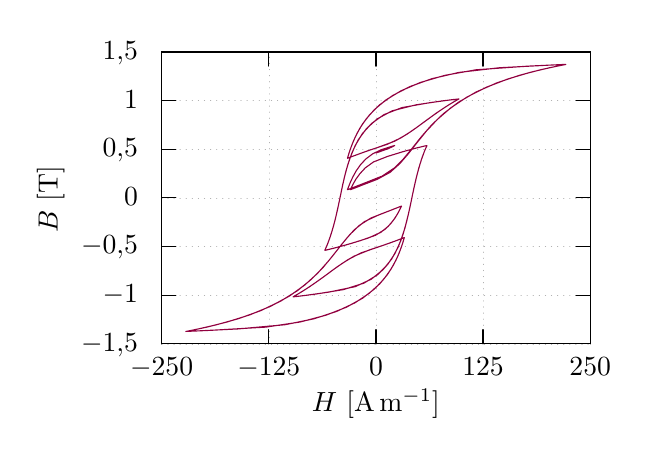
\begin{tikzpicture}[gnuplot]
%% generated with GNUPLOT 5.4p2 (Lua 5.4; terminal rev. Jun 2020, script rev. 114)
%% Fri 23 May 2025 09:04:29 AM -03
\path (0.000,0.000) rectangle (7.500,5.000);
\gpcolor{color=gp lt color axes}
\gpsetlinetype{gp lt axes}
\gpsetdashtype{gp dt axes}
\gpsetlinewidth{0.50}
\draw[gp path] (1.504,0.985)--(6.947,0.985);
\gpcolor{color=gp lt color border}
\gpsetlinetype{gp lt border}
\gpsetdashtype{gp dt solid}
\gpsetlinewidth{1.00}
\draw[gp path] (1.504,0.985)--(1.684,0.985);
\draw[gp path] (6.947,0.985)--(6.767,0.985);
\node[gp node right] at (1.320,0.985) {$-1,5$};
\gpcolor{color=gp lt color axes}
\gpsetlinetype{gp lt axes}
\gpsetdashtype{gp dt axes}
\gpsetlinewidth{0.50}
\draw[gp path] (1.504,1.603)--(6.947,1.603);
\gpcolor{color=gp lt color border}
\gpsetlinetype{gp lt border}
\gpsetdashtype{gp dt solid}
\gpsetlinewidth{1.00}
\draw[gp path] (1.504,1.603)--(1.684,1.603);
\draw[gp path] (6.947,1.603)--(6.767,1.603);
\node[gp node right] at (1.320,1.603) {$-1$};
\gpcolor{color=gp lt color axes}
\gpsetlinetype{gp lt axes}
\gpsetdashtype{gp dt axes}
\gpsetlinewidth{0.50}
\draw[gp path] (1.504,2.220)--(6.947,2.220);
\gpcolor{color=gp lt color border}
\gpsetlinetype{gp lt border}
\gpsetdashtype{gp dt solid}
\gpsetlinewidth{1.00}
\draw[gp path] (1.504,2.220)--(1.684,2.220);
\draw[gp path] (6.947,2.220)--(6.767,2.220);
\node[gp node right] at (1.320,2.220) {$-0,5$};
\gpcolor{color=gp lt color axes}
\gpsetlinetype{gp lt axes}
\gpsetdashtype{gp dt axes}
\gpsetlinewidth{0.50}
\draw[gp path] (1.504,2.838)--(6.947,2.838);
\gpcolor{color=gp lt color border}
\gpsetlinetype{gp lt border}
\gpsetdashtype{gp dt solid}
\gpsetlinewidth{1.00}
\draw[gp path] (1.504,2.838)--(1.684,2.838);
\draw[gp path] (6.947,2.838)--(6.767,2.838);
\node[gp node right] at (1.320,2.838) {$0$};
\gpcolor{color=gp lt color axes}
\gpsetlinetype{gp lt axes}
\gpsetdashtype{gp dt axes}
\gpsetlinewidth{0.50}
\draw[gp path] (1.504,3.456)--(6.947,3.456);
\gpcolor{color=gp lt color border}
\gpsetlinetype{gp lt border}
\gpsetdashtype{gp dt solid}
\gpsetlinewidth{1.00}
\draw[gp path] (1.504,3.456)--(1.684,3.456);
\draw[gp path] (6.947,3.456)--(6.767,3.456);
\node[gp node right] at (1.320,3.456) {$0,5$};
\gpcolor{color=gp lt color axes}
\gpsetlinetype{gp lt axes}
\gpsetdashtype{gp dt axes}
\gpsetlinewidth{0.50}
\draw[gp path] (1.504,4.073)--(6.947,4.073);
\gpcolor{color=gp lt color border}
\gpsetlinetype{gp lt border}
\gpsetdashtype{gp dt solid}
\gpsetlinewidth{1.00}
\draw[gp path] (1.504,4.073)--(1.684,4.073);
\draw[gp path] (6.947,4.073)--(6.767,4.073);
\node[gp node right] at (1.320,4.073) {$1$};
\gpcolor{color=gp lt color axes}
\gpsetlinetype{gp lt axes}
\gpsetdashtype{gp dt axes}
\gpsetlinewidth{0.50}
\draw[gp path] (1.504,4.691)--(6.947,4.691);
\gpcolor{color=gp lt color border}
\gpsetlinetype{gp lt border}
\gpsetdashtype{gp dt solid}
\gpsetlinewidth{1.00}
\draw[gp path] (1.504,4.691)--(1.684,4.691);
\draw[gp path] (6.947,4.691)--(6.767,4.691);
\node[gp node right] at (1.320,4.691) {$1,5$};
\gpcolor{color=gp lt color axes}
\gpsetlinetype{gp lt axes}
\gpsetdashtype{gp dt axes}
\gpsetlinewidth{0.50}
\draw[gp path] (1.504,0.985)--(1.504,4.691);
\gpcolor{color=gp lt color border}
\gpsetlinetype{gp lt border}
\gpsetdashtype{gp dt solid}
\gpsetlinewidth{1.00}
\draw[gp path] (1.504,0.985)--(1.504,1.165);
\draw[gp path] (1.504,4.691)--(1.504,4.511);
\node[gp node center] at (1.504,0.677) {$-250$};
\gpcolor{color=gp lt color axes}
\gpsetlinetype{gp lt axes}
\gpsetdashtype{gp dt axes}
\gpsetlinewidth{0.50}
\draw[gp path] (2.865,0.985)--(2.865,4.691);
\gpcolor{color=gp lt color border}
\gpsetlinetype{gp lt border}
\gpsetdashtype{gp dt solid}
\gpsetlinewidth{1.00}
\draw[gp path] (2.865,0.985)--(2.865,1.165);
\draw[gp path] (2.865,4.691)--(2.865,4.511);
\node[gp node center] at (2.865,0.677) {$-125$};
\gpcolor{color=gp lt color axes}
\gpsetlinetype{gp lt axes}
\gpsetdashtype{gp dt axes}
\gpsetlinewidth{0.50}
\draw[gp path] (4.226,0.985)--(4.226,4.691);
\gpcolor{color=gp lt color border}
\gpsetlinetype{gp lt border}
\gpsetdashtype{gp dt solid}
\gpsetlinewidth{1.00}
\draw[gp path] (4.226,0.985)--(4.226,1.165);
\draw[gp path] (4.226,4.691)--(4.226,4.511);
\node[gp node center] at (4.226,0.677) {$0$};
\gpcolor{color=gp lt color axes}
\gpsetlinetype{gp lt axes}
\gpsetdashtype{gp dt axes}
\gpsetlinewidth{0.50}
\draw[gp path] (5.586,0.985)--(5.586,4.691);
\gpcolor{color=gp lt color border}
\gpsetlinetype{gp lt border}
\gpsetdashtype{gp dt solid}
\gpsetlinewidth{1.00}
\draw[gp path] (5.586,0.985)--(5.586,1.165);
\draw[gp path] (5.586,4.691)--(5.586,4.511);
\node[gp node center] at (5.586,0.677) {$125$};
\gpcolor{color=gp lt color axes}
\gpsetlinetype{gp lt axes}
\gpsetdashtype{gp dt axes}
\gpsetlinewidth{0.50}
\draw[gp path] (6.947,0.985)--(6.947,4.691);
\gpcolor{color=gp lt color border}
\gpsetlinetype{gp lt border}
\gpsetdashtype{gp dt solid}
\gpsetlinewidth{1.00}
\draw[gp path] (6.947,0.985)--(6.947,1.165);
\draw[gp path] (6.947,4.691)--(6.947,4.511);
\node[gp node center] at (6.947,0.677) {$250$};
\draw[gp path] (1.504,4.691)--(1.504,0.985)--(6.947,0.985)--(6.947,4.691)--cycle;
\node[gp node center,rotate=-270] at (0.108,2.838) {$B$ [\si{\tesla}]};
\node[gp node center] at (4.225,0.215) {$H$ [\si{\ampere\per\meter}]};
\gpcolor{rgb color={0.569,0.000,0.247}}
\draw[gp path] (4.226,3.408)--(4.387,3.465)--(4.453,3.497)--(4.464,3.504)--(4.409,3.487)%
  --(4.293,3.450)--(4.183,3.397)--(4.096,3.331)--(4.028,3.257)--(3.975,3.181)--(3.935,3.109)%
  --(3.904,3.044)--(3.883,2.992)--(3.869,2.957)--(3.864,2.942)--(3.884,2.949)--(3.965,2.981)%
  --(4.108,3.037)--(4.307,3.116)--(4.457,3.216)--(4.576,3.335)--(4.686,3.468)--(4.800,3.612)%
  --(4.929,3.760)--(5.083,3.908)--(5.271,4.051)--(5.496,4.182)--(5.759,4.298)--(6.044,4.394)%
  --(6.319,4.466)--(6.535,4.513)--(6.637,4.533)--(6.442,4.525)--(5.792,4.491)--(5.281,4.432)%
  --(4.936,4.352)--(4.660,4.253)--(4.442,4.141)--(4.274,4.021)--(4.148,3.897)--(4.055,3.776)%
  --(3.988,3.662)--(3.940,3.560)--(3.907,3.474)--(3.884,3.408)--(3.871,3.364)--(3.865,3.343)%
  --(3.876,3.346)--(3.942,3.371)--(4.067,3.417)--(4.252,3.480)--(4.464,3.558)--(4.617,3.645)%
  --(4.748,3.736)--(4.871,3.827)--(4.988,3.912)--(5.097,3.985)--(5.189,4.043)--(5.253,4.080)%
  --(5.280,4.095)--(5.189,4.085)--(4.913,4.048)--(4.556,3.985)--(4.328,3.896)--(4.170,3.783)%
  --(4.051,3.651)--(3.962,3.502)--(3.895,3.342)--(3.844,3.175)--(3.804,3.007)--(3.770,2.843)%
  --(3.738,2.689)--(3.705,2.549)--(3.671,2.427)--(3.639,2.327)--(3.611,2.251)--(3.589,2.200)%
  --(3.578,2.175)--(3.588,2.174)--(3.679,2.196)--(3.836,2.238)--(4.027,2.295)--(4.220,2.363)%
  --(4.339,2.438)--(4.415,2.513)--(4.469,2.584)--(4.506,2.646)--(4.532,2.695)--(4.546,2.725)%
  --(4.551,2.734)--(4.516,2.721)--(4.419,2.683)--(4.261,2.622)--(4.080,2.537)--(3.950,2.432)%
  --(3.840,2.309)--(3.732,2.173)--(3.616,2.028)--(3.483,1.879)--(3.322,1.732)--(3.126,1.591)%
  --(2.891,1.463)--(2.622,1.352)--(2.335,1.262)--(2.070,1.195)--(1.878,1.155)--(1.811,1.142)%
  --(2.143,1.157)--(2.827,1.197)--(3.264,1.262)--(3.590,1.348)--(3.851,1.450)--(4.056,1.564)%
  --(4.212,1.686)--(4.329,1.810)--(4.415,1.930)--(4.477,2.041)--(4.521,2.139)--(4.551,2.220)%
  --(4.571,2.281)--(4.582,2.319)--(4.586,2.334)--(4.564,2.326)--(4.483,2.295)--(4.344,2.245)%
  --(4.142,2.177)--(3.945,2.097)--(3.800,2.008)--(3.671,1.917)--(3.550,1.827)--(3.434,1.745)%
  --(3.329,1.675)--(3.243,1.622)--(3.187,1.590)--(3.174,1.581)--(3.317,1.598)--(3.625,1.641)%
  --(3.963,1.711)--(4.167,1.806)--(4.314,1.924)--(4.425,2.061)--(4.508,2.213)--(4.570,2.375)%
  --(4.617,2.543)--(4.656,2.711)--(4.689,2.872)--(4.722,3.024)--(4.755,3.159)--(4.788,3.276)%
  --(4.819,3.370)--(4.846,3.440)--(4.865,3.484)--(4.874,3.503)--(4.848,3.498)--(4.737,3.471)%
  --(4.569,3.425)--(4.374,3.365)--(4.195,3.295)--(4.090,3.219)--(4.021,3.144)--(3.971,3.075)%
  --(3.937,3.016)--(3.915,2.972)--(3.902,2.947)--(3.903,2.943)--(3.954,2.962)--(4.065,3.006)%
  --(4.240,3.073)--(4.406,3.163)--(4.529,3.273)--(4.638,3.400)--(4.747,3.539)--(4.866,3.686)%
  --(5.005,3.834)--(5.174,3.980)--(5.380,4.118)--(5.624,4.242)--(5.900,4.348)--(6.186,4.433)%
  --(6.438,4.493)--(6.603,4.526)--(6.614,4.533)--(6.150,4.511)--(5.496,4.465)--(5.098,4.394)%
  --(4.790,4.304)--(4.544,4.198)--(4.352,4.082)--(4.206,3.959)--(4.098,3.836)--(4.019,3.718)%
  --(3.962,3.609)--(3.922,3.515)--(3.894,3.439)--(3.877,3.383)--(3.867,3.351)--(3.865,3.341)%
  --(3.902,3.356)--(3.997,3.391)--(4.152,3.447)--(4.368,3.518)--(4.545,3.601)--(4.684,3.690)%
  --(4.811,3.782)--(4.931,3.870)--(5.044,3.950)--(5.145,4.016)--(5.225,4.064)--(5.272,4.091)%
  --(5.261,4.093)--(5.069,4.070)--(4.734,4.020)--(4.429,3.943)--(4.243,3.842)--(4.107,3.720)%
  --(4.003,3.578)--(3.926,3.423)--(3.868,3.259)--(3.823,3.091)--(3.787,2.924)--(3.754,2.765)%
  --(3.721,2.617)--(3.688,2.485)--(3.655,2.374)--(3.624,2.286)--(3.599,2.223)--(3.582,2.185)%
  --(3.577,2.172)--(3.623,2.183)--(3.751,2.215)--(3.929,2.265)--(4.128,2.328)--(4.287,2.400)%
  --(4.381,2.476)--(4.444,2.550)--(4.489,2.617)--(4.521,2.673)--(4.540,2.712)--(4.550,2.733)%
  --(4.541,2.731)--(4.475,2.705)--(4.348,2.655)--(4.161,2.582)--(4.012,2.487)--(3.894,2.372)%
  --(3.786,2.242)--(3.676,2.101)--(3.553,1.953)--(3.407,1.805)--(3.229,1.660)--(3.014,1.526)%
  --(2.760,1.405)--(2.479,1.304)--(2.197,1.226)--(1.961,1.172)--(1.827,1.145)--(1.905,1.146)%
  --(2.475,1.174)--(3.068,1.227)--(3.437,1.302)--(3.728,1.397)--(3.960,1.506)--(4.139,1.625)%
  --(4.275,1.748)--(4.376,1.870)--(4.449,1.987)--(4.501,2.092)--(4.537,2.182)--(4.562,2.253)%
  --(4.577,2.303)--(4.585,2.330)--(4.582,2.333)--(4.531,2.313)--(4.421,2.272)--(4.251,2.213)%
  --(4.032,2.138)--(3.869,2.053)--(3.734,1.963)--(3.610,1.871)--(3.491,1.785)--(3.380,1.708)%
  --(3.283,1.646)--(3.211,1.603)--(3.174,1.582)--(3.220,1.586)--(3.457,1.616)--(3.812,1.673)%
  --(4.075,1.756)--(4.246,1.862)--(4.373,1.990)--(4.469,2.135)--(4.541,2.293)--(4.595,2.459)%
  --(4.637,2.627)--(4.673,2.793)--(4.705,2.950)--(4.738,3.094)--(4.771,3.220)--(4.804,3.326)%
  --(4.834,3.408);
\gpcolor{color=gp lt color border}
\draw[gp path] (1.504,4.691)--(1.504,0.985)--(6.947,0.985)--(6.947,4.691)--cycle;
%% coordinates of the plot area
\gpdefrectangularnode{gp plot 1}{\pgfpoint{1.504cm}{0.985cm}}{\pgfpoint{6.947cm}{4.691cm}}
\end{tikzpicture}
%% gnuplot variables

    \vspace{-1cm}
    \caption{uma caption}
  \end{minipage}%
  \begin{minipage}{.49\linewidth}
    \centering
    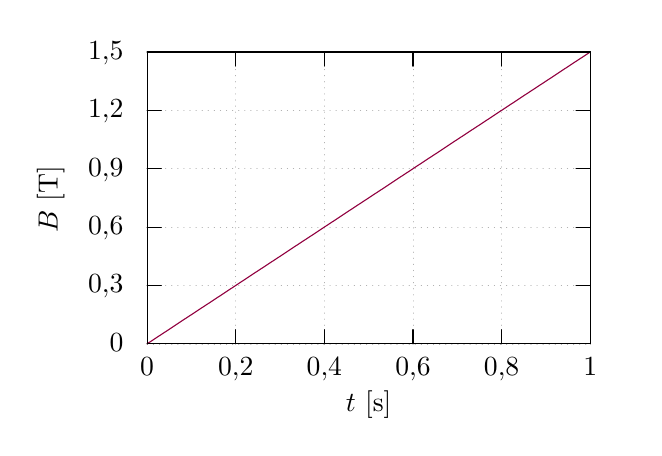
\begin{tikzpicture}[gnuplot]
%% generated with GNUPLOT 5.4p2 (Lua 5.4; terminal rev. Jun 2020, script rev. 114)
%% Fri 23 May 2025 09:06:32 AM -03
\path (0.000,0.000) rectangle (7.500,5.000);
\gpcolor{color=gp lt color axes}
\gpsetlinetype{gp lt axes}
\gpsetdashtype{gp dt axes}
\gpsetlinewidth{0.50}
\draw[gp path] (1.320,0.985)--(6.947,0.985);
\gpcolor{color=gp lt color border}
\gpsetlinetype{gp lt border}
\gpsetdashtype{gp dt solid}
\gpsetlinewidth{1.00}
\draw[gp path] (1.320,0.985)--(1.500,0.985);
\draw[gp path] (6.947,0.985)--(6.767,0.985);
\node[gp node right] at (1.136,0.985) {$0$};
\gpcolor{color=gp lt color axes}
\gpsetlinetype{gp lt axes}
\gpsetdashtype{gp dt axes}
\gpsetlinewidth{0.50}
\draw[gp path] (1.320,1.726)--(6.947,1.726);
\gpcolor{color=gp lt color border}
\gpsetlinetype{gp lt border}
\gpsetdashtype{gp dt solid}
\gpsetlinewidth{1.00}
\draw[gp path] (1.320,1.726)--(1.500,1.726);
\draw[gp path] (6.947,1.726)--(6.767,1.726);
\node[gp node right] at (1.136,1.726) {$0,3$};
\gpcolor{color=gp lt color axes}
\gpsetlinetype{gp lt axes}
\gpsetdashtype{gp dt axes}
\gpsetlinewidth{0.50}
\draw[gp path] (1.320,2.467)--(6.947,2.467);
\gpcolor{color=gp lt color border}
\gpsetlinetype{gp lt border}
\gpsetdashtype{gp dt solid}
\gpsetlinewidth{1.00}
\draw[gp path] (1.320,2.467)--(1.500,2.467);
\draw[gp path] (6.947,2.467)--(6.767,2.467);
\node[gp node right] at (1.136,2.467) {$0,6$};
\gpcolor{color=gp lt color axes}
\gpsetlinetype{gp lt axes}
\gpsetdashtype{gp dt axes}
\gpsetlinewidth{0.50}
\draw[gp path] (1.320,3.209)--(6.947,3.209);
\gpcolor{color=gp lt color border}
\gpsetlinetype{gp lt border}
\gpsetdashtype{gp dt solid}
\gpsetlinewidth{1.00}
\draw[gp path] (1.320,3.209)--(1.500,3.209);
\draw[gp path] (6.947,3.209)--(6.767,3.209);
\node[gp node right] at (1.136,3.209) {$0,9$};
\gpcolor{color=gp lt color axes}
\gpsetlinetype{gp lt axes}
\gpsetdashtype{gp dt axes}
\gpsetlinewidth{0.50}
\draw[gp path] (1.320,3.950)--(6.947,3.950);
\gpcolor{color=gp lt color border}
\gpsetlinetype{gp lt border}
\gpsetdashtype{gp dt solid}
\gpsetlinewidth{1.00}
\draw[gp path] (1.320,3.950)--(1.500,3.950);
\draw[gp path] (6.947,3.950)--(6.767,3.950);
\node[gp node right] at (1.136,3.950) {$1,2$};
\gpcolor{color=gp lt color axes}
\gpsetlinetype{gp lt axes}
\gpsetdashtype{gp dt axes}
\gpsetlinewidth{0.50}
\draw[gp path] (1.320,4.691)--(6.947,4.691);
\gpcolor{color=gp lt color border}
\gpsetlinetype{gp lt border}
\gpsetdashtype{gp dt solid}
\gpsetlinewidth{1.00}
\draw[gp path] (1.320,4.691)--(1.500,4.691);
\draw[gp path] (6.947,4.691)--(6.767,4.691);
\node[gp node right] at (1.136,4.691) {$1,5$};
\gpcolor{color=gp lt color axes}
\gpsetlinetype{gp lt axes}
\gpsetdashtype{gp dt axes}
\gpsetlinewidth{0.50}
\draw[gp path] (1.320,0.985)--(1.320,4.691);
\gpcolor{color=gp lt color border}
\gpsetlinetype{gp lt border}
\gpsetdashtype{gp dt solid}
\gpsetlinewidth{1.00}
\draw[gp path] (1.320,0.985)--(1.320,1.165);
\draw[gp path] (1.320,4.691)--(1.320,4.511);
\node[gp node center] at (1.320,0.677) {$0$};
\gpcolor{color=gp lt color axes}
\gpsetlinetype{gp lt axes}
\gpsetdashtype{gp dt axes}
\gpsetlinewidth{0.50}
\draw[gp path] (2.445,0.985)--(2.445,4.691);
\gpcolor{color=gp lt color border}
\gpsetlinetype{gp lt border}
\gpsetdashtype{gp dt solid}
\gpsetlinewidth{1.00}
\draw[gp path] (2.445,0.985)--(2.445,1.165);
\draw[gp path] (2.445,4.691)--(2.445,4.511);
\node[gp node center] at (2.445,0.677) {$0,2$};
\gpcolor{color=gp lt color axes}
\gpsetlinetype{gp lt axes}
\gpsetdashtype{gp dt axes}
\gpsetlinewidth{0.50}
\draw[gp path] (3.571,0.985)--(3.571,4.691);
\gpcolor{color=gp lt color border}
\gpsetlinetype{gp lt border}
\gpsetdashtype{gp dt solid}
\gpsetlinewidth{1.00}
\draw[gp path] (3.571,0.985)--(3.571,1.165);
\draw[gp path] (3.571,4.691)--(3.571,4.511);
\node[gp node center] at (3.571,0.677) {$0,4$};
\gpcolor{color=gp lt color axes}
\gpsetlinetype{gp lt axes}
\gpsetdashtype{gp dt axes}
\gpsetlinewidth{0.50}
\draw[gp path] (4.696,0.985)--(4.696,4.691);
\gpcolor{color=gp lt color border}
\gpsetlinetype{gp lt border}
\gpsetdashtype{gp dt solid}
\gpsetlinewidth{1.00}
\draw[gp path] (4.696,0.985)--(4.696,1.165);
\draw[gp path] (4.696,4.691)--(4.696,4.511);
\node[gp node center] at (4.696,0.677) {$0,6$};
\gpcolor{color=gp lt color axes}
\gpsetlinetype{gp lt axes}
\gpsetdashtype{gp dt axes}
\gpsetlinewidth{0.50}
\draw[gp path] (5.822,0.985)--(5.822,4.691);
\gpcolor{color=gp lt color border}
\gpsetlinetype{gp lt border}
\gpsetdashtype{gp dt solid}
\gpsetlinewidth{1.00}
\draw[gp path] (5.822,0.985)--(5.822,1.165);
\draw[gp path] (5.822,4.691)--(5.822,4.511);
\node[gp node center] at (5.822,0.677) {$0,8$};
\gpcolor{color=gp lt color axes}
\gpsetlinetype{gp lt axes}
\gpsetdashtype{gp dt axes}
\gpsetlinewidth{0.50}
\draw[gp path] (6.947,0.985)--(6.947,4.691);
\gpcolor{color=gp lt color border}
\gpsetlinetype{gp lt border}
\gpsetdashtype{gp dt solid}
\gpsetlinewidth{1.00}
\draw[gp path] (6.947,0.985)--(6.947,1.165);
\draw[gp path] (6.947,4.691)--(6.947,4.511);
\node[gp node center] at (6.947,0.677) {$1$};
\draw[gp path] (1.320,4.691)--(1.320,0.985)--(6.947,0.985)--(6.947,4.691)--cycle;
\node[gp node center,rotate=-270] at (0.108,2.838) {$B$ [\si{\tesla}]};
\node[gp node center] at (4.133,0.215) {$t$ [\si{\second}]};
\gpcolor{rgb color={0.569,0.000,0.247}}
\draw[gp path] (1.320,0.985)--(1.435,1.061)--(1.550,1.136)--(1.665,1.212)--(1.779,1.288)%
  --(1.894,1.363)--(2.009,1.439)--(2.124,1.514)--(2.239,1.590)--(2.354,1.666)--(2.468,1.741)%
  --(2.583,1.817)--(2.698,1.893)--(2.813,1.968)--(2.928,2.044)--(3.043,2.119)--(3.157,2.195)%
  --(3.272,2.271)--(3.387,2.346)--(3.502,2.422)--(3.617,2.498)--(3.732,2.573)--(3.846,2.649)%
  --(3.961,2.725)--(4.076,2.800)--(4.191,2.876)--(4.306,2.951)--(4.421,3.027)--(4.535,3.103)%
  --(4.650,3.178)--(4.765,3.254)--(4.880,3.330)--(4.995,3.405)--(5.110,3.481)--(5.224,3.557)%
  --(5.339,3.632)--(5.454,3.708)--(5.569,3.783)--(5.684,3.859)--(5.799,3.935)--(5.913,4.010)%
  --(6.028,4.086)--(6.143,4.162)--(6.258,4.237)--(6.373,4.313)--(6.488,4.388)--(6.602,4.464)%
  --(6.717,4.540)--(6.832,4.615)--(6.947,4.691);
\gpcolor{color=gp lt color border}
\draw[gp path] (1.320,4.691)--(1.320,0.985)--(6.947,0.985)--(6.947,4.691)--cycle;
%% coordinates of the plot area
\gpdefrectangularnode{gp plot 1}{\pgfpoint{1.320cm}{0.985cm}}{\pgfpoint{6.947cm}{4.691cm}}
\end{tikzpicture}
%% gnuplot variables

    \vspace{-1cm}
    \caption{HHHHHHHHHHHHHHH}
  \end{minipage}
  \begin{minipage}{.49\linewidth}
    \centering
    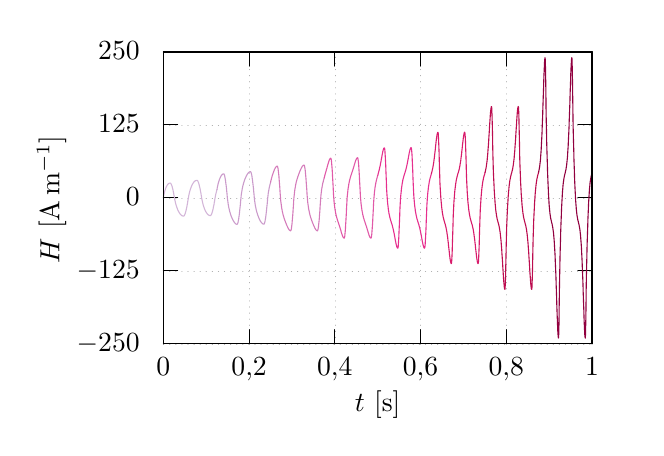
\begin{tikzpicture}[gnuplot]
%% generated with GNUPLOT 5.4p2 (Lua 5.4; terminal rev. Jun 2020, script rev. 114)
%% Fri 23 May 2025 09:05:47 AM -03
\path (0.000,0.000) rectangle (7.500,5.000);
\gpcolor{color=gp lt color axes}
\gpsetlinetype{gp lt axes}
\gpsetdashtype{gp dt axes}
\gpsetlinewidth{0.50}
\draw[gp path] (1.504,0.985)--(6.947,0.985);
\gpcolor{color=gp lt color border}
\gpsetlinetype{gp lt border}
\gpsetdashtype{gp dt solid}
\gpsetlinewidth{1.00}
\draw[gp path] (1.504,0.985)--(1.684,0.985);
\draw[gp path] (6.947,0.985)--(6.767,0.985);
\node[gp node right] at (1.320,0.985) {$-250$};
\gpcolor{color=gp lt color axes}
\gpsetlinetype{gp lt axes}
\gpsetdashtype{gp dt axes}
\gpsetlinewidth{0.50}
\draw[gp path] (1.504,1.912)--(6.947,1.912);
\gpcolor{color=gp lt color border}
\gpsetlinetype{gp lt border}
\gpsetdashtype{gp dt solid}
\gpsetlinewidth{1.00}
\draw[gp path] (1.504,1.912)--(1.684,1.912);
\draw[gp path] (6.947,1.912)--(6.767,1.912);
\node[gp node right] at (1.320,1.912) {$-125$};
\gpcolor{color=gp lt color axes}
\gpsetlinetype{gp lt axes}
\gpsetdashtype{gp dt axes}
\gpsetlinewidth{0.50}
\draw[gp path] (1.504,2.838)--(6.947,2.838);
\gpcolor{color=gp lt color border}
\gpsetlinetype{gp lt border}
\gpsetdashtype{gp dt solid}
\gpsetlinewidth{1.00}
\draw[gp path] (1.504,2.838)--(1.684,2.838);
\draw[gp path] (6.947,2.838)--(6.767,2.838);
\node[gp node right] at (1.320,2.838) {$0$};
\gpcolor{color=gp lt color axes}
\gpsetlinetype{gp lt axes}
\gpsetdashtype{gp dt axes}
\gpsetlinewidth{0.50}
\draw[gp path] (1.504,3.765)--(6.947,3.765);
\gpcolor{color=gp lt color border}
\gpsetlinetype{gp lt border}
\gpsetdashtype{gp dt solid}
\gpsetlinewidth{1.00}
\draw[gp path] (1.504,3.765)--(1.684,3.765);
\draw[gp path] (6.947,3.765)--(6.767,3.765);
\node[gp node right] at (1.320,3.765) {$125$};
\gpcolor{color=gp lt color axes}
\gpsetlinetype{gp lt axes}
\gpsetdashtype{gp dt axes}
\gpsetlinewidth{0.50}
\draw[gp path] (1.504,4.691)--(6.947,4.691);
\gpcolor{color=gp lt color border}
\gpsetlinetype{gp lt border}
\gpsetdashtype{gp dt solid}
\gpsetlinewidth{1.00}
\draw[gp path] (1.504,4.691)--(1.684,4.691);
\draw[gp path] (6.947,4.691)--(6.767,4.691);
\node[gp node right] at (1.320,4.691) {$250$};
\gpcolor{color=gp lt color axes}
\gpsetlinetype{gp lt axes}
\gpsetdashtype{gp dt axes}
\gpsetlinewidth{0.50}
\draw[gp path] (1.504,0.985)--(1.504,4.691);
\gpcolor{color=gp lt color border}
\gpsetlinetype{gp lt border}
\gpsetdashtype{gp dt solid}
\gpsetlinewidth{1.00}
\draw[gp path] (1.504,0.985)--(1.504,1.165);
\draw[gp path] (1.504,4.691)--(1.504,4.511);
\node[gp node center] at (1.504,0.677) {$0$};
\gpcolor{color=gp lt color axes}
\gpsetlinetype{gp lt axes}
\gpsetdashtype{gp dt axes}
\gpsetlinewidth{0.50}
\draw[gp path] (2.593,0.985)--(2.593,4.691);
\gpcolor{color=gp lt color border}
\gpsetlinetype{gp lt border}
\gpsetdashtype{gp dt solid}
\gpsetlinewidth{1.00}
\draw[gp path] (2.593,0.985)--(2.593,1.165);
\draw[gp path] (2.593,4.691)--(2.593,4.511);
\node[gp node center] at (2.593,0.677) {$0,2$};
\gpcolor{color=gp lt color axes}
\gpsetlinetype{gp lt axes}
\gpsetdashtype{gp dt axes}
\gpsetlinewidth{0.50}
\draw[gp path] (3.681,0.985)--(3.681,4.691);
\gpcolor{color=gp lt color border}
\gpsetlinetype{gp lt border}
\gpsetdashtype{gp dt solid}
\gpsetlinewidth{1.00}
\draw[gp path] (3.681,0.985)--(3.681,1.165);
\draw[gp path] (3.681,4.691)--(3.681,4.511);
\node[gp node center] at (3.681,0.677) {$0,4$};
\gpcolor{color=gp lt color axes}
\gpsetlinetype{gp lt axes}
\gpsetdashtype{gp dt axes}
\gpsetlinewidth{0.50}
\draw[gp path] (4.770,0.985)--(4.770,4.691);
\gpcolor{color=gp lt color border}
\gpsetlinetype{gp lt border}
\gpsetdashtype{gp dt solid}
\gpsetlinewidth{1.00}
\draw[gp path] (4.770,0.985)--(4.770,1.165);
\draw[gp path] (4.770,4.691)--(4.770,4.511);
\node[gp node center] at (4.770,0.677) {$0,6$};
\gpcolor{color=gp lt color axes}
\gpsetlinetype{gp lt axes}
\gpsetdashtype{gp dt axes}
\gpsetlinewidth{0.50}
\draw[gp path] (5.858,0.985)--(5.858,4.691);
\gpcolor{color=gp lt color border}
\gpsetlinetype{gp lt border}
\gpsetdashtype{gp dt solid}
\gpsetlinewidth{1.00}
\draw[gp path] (5.858,0.985)--(5.858,1.165);
\draw[gp path] (5.858,4.691)--(5.858,4.511);
\node[gp node center] at (5.858,0.677) {$0,8$};
\gpcolor{color=gp lt color axes}
\gpsetlinetype{gp lt axes}
\gpsetdashtype{gp dt axes}
\gpsetlinewidth{0.50}
\draw[gp path] (6.947,0.985)--(6.947,4.691);
\gpcolor{color=gp lt color border}
\gpsetlinetype{gp lt border}
\gpsetdashtype{gp dt solid}
\gpsetlinewidth{1.00}
\draw[gp path] (6.947,0.985)--(6.947,1.165);
\draw[gp path] (6.947,4.691)--(6.947,4.511);
\node[gp node center] at (6.947,0.677) {$1$};
\draw[gp path] (1.504,4.691)--(1.504,0.985)--(6.947,0.985)--(6.947,4.691)--cycle;
\node[gp node center,rotate=-270] at (0.108,2.838) {$H$ [\si{\ampere\per\meter}]};
\node[gp node center] at (4.225,0.215) {$t$ [\si{\second}]};
\gpcolor{rgb color={0.827,0.711,0.847}}
\draw[gp path] (1.504,2.838)--(1.507,2.856)--(1.509,2.871)--(1.512,2.885)--(1.515,2.898)%
  --(1.518,2.909)--(1.520,2.920)--(1.523,2.929)--(1.526,2.938)--(1.529,2.947)--(1.531,2.955)%
  --(1.534,2.962)--(1.537,2.969)--(1.539,2.975)--(1.542,2.981)--(1.545,2.986)--(1.548,2.991)%
  --(1.550,2.996)--(1.553,3.000)--(1.556,3.004)--(1.558,3.008)--(1.561,3.011)--(1.564,3.014)%
  --(1.567,3.016)--(1.569,3.019)--(1.572,3.021)--(1.575,3.022)--(1.578,3.024)--(1.580,3.025)%
  --(1.583,3.026)--(1.586,3.026)--(1.588,3.027)--(1.591,3.026)--(1.594,3.025)--(1.597,3.023)%
  --(1.599,3.019)--(1.602,3.015)--(1.605,3.009)--(1.607,3.003)--(1.610,2.996)--(1.613,2.988)%
  --(1.616,2.979)--(1.618,2.969)--(1.621,2.958)--(1.624,2.947)--(1.627,2.935)--(1.629,2.922)%
  --(1.632,2.908)--(1.635,2.894)--(1.637,2.879)--(1.640,2.864)--(1.643,2.848)--(1.646,2.833)%
  --(1.648,2.818)--(1.651,2.805)--(1.654,2.793)--(1.656,2.781)--(1.659,2.770)--(1.662,2.760)%
  --(1.665,2.750)--(1.667,2.741)--(1.670,2.732)--(1.673,2.724)--(1.676,2.716)--(1.678,2.709)%
  --(1.681,2.701)--(1.684,2.695)--(1.686,2.688)--(1.689,2.682)--(1.692,2.676)--(1.695,2.670)%
  --(1.697,2.665)--(1.700,2.660)--(1.703,2.655)--(1.705,2.650)--(1.708,2.646)--(1.711,2.642)%
  --(1.714,2.638)--(1.716,2.635)--(1.719,2.631)--(1.722,2.628)--(1.725,2.625)--(1.727,2.622)%
  --(1.730,2.620)--(1.733,2.618)--(1.735,2.616)--(1.738,2.614)--(1.741,2.612)--(1.744,2.611)%
  --(1.746,2.610)--(1.749,2.609)--(1.752,2.608)--(1.755,2.607)--(1.757,2.607)--(1.760,2.607)%
  --(1.763,2.608)--(1.765,2.610)--(1.768,2.613)--(1.771,2.617)--(1.774,2.622)--(1.776,2.628)%
  --(1.779,2.635)--(1.782,2.643)--(1.784,2.651)--(1.787,2.661)--(1.790,2.672)--(1.793,2.683)%
  --(1.795,2.695)--(1.798,2.708)--(1.801,2.721)--(1.804,2.735)--(1.806,2.750)--(1.809,2.765)%
  --(1.812,2.780)--(1.814,2.796)--(1.817,2.813)--(1.820,2.830)--(1.823,2.847)--(1.825,2.861)%
  --(1.828,2.875)--(1.831,2.888)--(1.833,2.899)--(1.836,2.910)--(1.839,2.921)--(1.842,2.930)%
  --(1.844,2.940)--(1.847,2.948)--(1.850,2.956)--(1.853,2.964)--(1.855,2.972)--(1.858,2.978)%
  --(1.861,2.985)--(1.863,2.991)--(1.866,2.997)--(1.869,3.003)--(1.872,3.008)--(1.874,3.013)%
  --(1.877,3.018)--(1.880,3.023)--(1.882,3.027)--(1.885,3.031)--(1.888,3.035)--(1.891,3.038)%
  --(1.893,3.041)--(1.896,3.044)--(1.899,3.047)--(1.902,3.049)--(1.904,3.052)--(1.907,3.054)%
  --(1.910,3.055)--(1.912,3.057)--(1.915,3.058)--(1.918,3.059)--(1.921,3.060)--(1.923,3.061)%
  --(1.926,3.061)--(1.929,3.061)--(1.931,3.061)--(1.934,3.060)--(1.937,3.057)--(1.940,3.054)%
  --(1.942,3.049)--(1.945,3.044)--(1.948,3.037)--(1.951,3.030)--(1.953,3.022)--(1.956,3.012)%
  --(1.959,3.002)--(1.961,2.991)--(1.964,2.980)--(1.967,2.967)--(1.970,2.954)--(1.972,2.941)%
  --(1.975,2.926)--(1.978,2.911)--(1.981,2.896)--(1.983,2.880)--(1.986,2.864)--(1.989,2.847)%
  --(1.991,2.831)--(1.994,2.816)--(1.997,2.802)--(2.000,2.789)--(2.002,2.778)--(2.005,2.767)%
  --(2.008,2.756)--(2.010,2.747)--(2.013,2.737)--(2.016,2.729)--(2.019,2.721)--(2.021,2.713)%
  --(2.024,2.705)--(2.027,2.698)--(2.030,2.692)--(2.032,2.685)--(2.035,2.679)--(2.038,2.674)%
  --(2.040,2.668)--(2.043,2.663)--(2.046,2.658)--(2.049,2.654)--(2.051,2.649)--(2.054,2.645)%
  --(2.057,2.642)--(2.059,2.638)--(2.062,2.635)--(2.065,2.632)--(2.068,2.629)--(2.070,2.626)%
  --(2.073,2.624)--(2.076,2.622)--(2.079,2.620)--(2.081,2.618)--(2.084,2.617)--(2.087,2.616)%
  --(2.089,2.615)--(2.092,2.614)--(2.095,2.614)--(2.098,2.613)--(2.100,2.613)--(2.103,2.614)%
  --(2.106,2.616)--(2.108,2.619)--(2.111,2.623)--(2.114,2.628)--(2.117,2.634)--(2.119,2.641)%
  --(2.122,2.649)--(2.125,2.658)--(2.128,2.668)--(2.130,2.678)--(2.133,2.689)--(2.136,2.701)%
  --(2.138,2.714)--(2.141,2.728)--(2.144,2.742)--(2.147,2.756)--(2.149,2.771)--(2.152,2.787)%
  --(2.155,2.803)--(2.157,2.820)--(2.160,2.837)--(2.163,2.852)--(2.166,2.867)--(2.168,2.880)%
  --(2.171,2.892)--(2.174,2.904)--(2.177,2.914)--(2.179,2.924)--(2.182,2.934)--(2.185,2.944);
\gpcolor{rgb color={0.797,0.609,0.795}}
\draw[gp path] (2.185,2.944)--(2.187,2.960)--(2.190,2.975)--(2.193,2.989)--(2.196,3.001)%
  --(2.198,3.013)--(2.201,3.024)--(2.204,3.034)--(2.206,3.043)--(2.209,3.052)--(2.212,3.060)%
  --(2.215,3.068)--(2.217,3.075)--(2.220,3.082)--(2.223,3.089)--(2.226,3.095)--(2.228,3.101)%
  --(2.231,3.106)--(2.234,3.111)--(2.236,3.116)--(2.239,3.120)--(2.242,3.124)--(2.245,3.128)%
  --(2.247,3.131)--(2.250,3.134)--(2.253,3.137)--(2.256,3.139)--(2.258,3.141)--(2.261,3.142)%
  --(2.264,3.143)--(2.266,3.144)--(2.269,3.144)--(2.272,3.143)--(2.275,3.140)--(2.277,3.134)%
  --(2.280,3.126)--(2.283,3.115)--(2.285,3.102)--(2.288,3.087)--(2.291,3.071)--(2.294,3.052)%
  --(2.296,3.032)--(2.299,3.010)--(2.302,2.986)--(2.305,2.961)--(2.307,2.935)--(2.310,2.908)%
  --(2.313,2.880)--(2.315,2.851)--(2.318,2.825)--(2.321,2.803)--(2.324,2.783)--(2.326,2.765)%
  --(2.329,2.748)--(2.332,2.733)--(2.334,2.719)--(2.337,2.706)--(2.340,2.694)--(2.343,2.682)%
  --(2.345,2.671)--(2.348,2.661)--(2.351,2.651)--(2.354,2.642)--(2.356,2.633)--(2.359,2.625)%
  --(2.362,2.617)--(2.364,2.609)--(2.367,2.602)--(2.370,2.595)--(2.373,2.589)--(2.375,2.582)%
  --(2.378,2.576)--(2.381,2.570)--(2.383,2.564)--(2.386,2.559)--(2.389,2.554)--(2.392,2.549)%
  --(2.394,2.544)--(2.397,2.540)--(2.400,2.535)--(2.403,2.531)--(2.405,2.527)--(2.408,2.524)%
  --(2.411,2.520)--(2.413,2.517)--(2.416,2.515)--(2.419,2.512)--(2.422,2.510)--(2.424,2.508)%
  --(2.427,2.506)--(2.430,2.505)--(2.432,2.504)--(2.435,2.503)--(2.438,2.503)--(2.441,2.503)%
  --(2.443,2.506)--(2.446,2.511)--(2.449,2.518)--(2.452,2.527)--(2.454,2.539)--(2.457,2.554)%
  --(2.460,2.570)--(2.462,2.588)--(2.465,2.608)--(2.468,2.629)--(2.471,2.653)--(2.473,2.677)%
  --(2.476,2.703)--(2.479,2.730)--(2.482,2.758)--(2.484,2.787)--(2.487,2.817)--(2.490,2.845)%
  --(2.492,2.869)--(2.495,2.890)--(2.498,2.908)--(2.501,2.925)--(2.503,2.941)--(2.506,2.956)%
  --(2.509,2.969)--(2.511,2.981)--(2.514,2.993)--(2.517,3.004)--(2.520,3.015)--(2.522,3.024)%
  --(2.525,3.034)--(2.528,3.043)--(2.531,3.051)--(2.533,3.059)--(2.536,3.067)--(2.539,3.074)%
  --(2.541,3.081)--(2.544,3.088)--(2.547,3.094)--(2.550,3.100)--(2.552,3.106)--(2.555,3.112)%
  --(2.558,3.117)--(2.560,3.122)--(2.563,3.127)--(2.566,3.132)--(2.569,3.137)--(2.571,3.141)%
  --(2.574,3.145)--(2.577,3.149)--(2.580,3.152)--(2.582,3.155)--(2.585,3.158)--(2.588,3.161)%
  --(2.590,3.163)--(2.593,3.165)--(2.596,3.167)--(2.599,3.169)--(2.601,3.170)--(2.604,3.171)%
  --(2.607,3.171)--(2.609,3.171)--(2.612,3.170)--(2.615,3.166)--(2.618,3.160)--(2.620,3.152)%
  --(2.623,3.141)--(2.626,3.128)--(2.629,3.112)--(2.631,3.095)--(2.634,3.076)--(2.637,3.055)%
  --(2.639,3.033)--(2.642,3.009)--(2.645,2.984)--(2.648,2.958)--(2.650,2.930)--(2.653,2.902)%
  --(2.656,2.872)--(2.658,2.843)--(2.661,2.817)--(2.664,2.795)--(2.667,2.775)--(2.669,2.758)%
  --(2.672,2.741)--(2.675,2.727)--(2.678,2.713)--(2.680,2.700)--(2.683,2.688)--(2.686,2.676)%
  --(2.688,2.666)--(2.691,2.656)--(2.694,2.646)--(2.697,2.637)--(2.699,2.629)--(2.702,2.620)%
  --(2.705,2.613)--(2.708,2.605)--(2.710,2.598)--(2.713,2.591)--(2.716,2.585)--(2.718,2.578)%
  --(2.721,2.572)--(2.724,2.567)--(2.727,2.561)--(2.729,2.556)--(2.732,2.551)--(2.735,2.546)%
  --(2.737,2.541)--(2.740,2.537)--(2.743,2.533)--(2.746,2.529)--(2.748,2.525)--(2.751,2.522)%
  --(2.754,2.519)--(2.757,2.516)--(2.759,2.514)--(2.762,2.511)--(2.765,2.510)--(2.767,2.508)%
  --(2.770,2.507)--(2.773,2.506)--(2.776,2.505)--(2.778,2.505)--(2.781,2.505)--(2.784,2.507)%
  --(2.786,2.512)--(2.789,2.520)--(2.792,2.530)--(2.795,2.542)--(2.797,2.556)--(2.800,2.572)%
  --(2.803,2.591)--(2.806,2.611)--(2.808,2.632)--(2.811,2.655)--(2.814,2.680)--(2.816,2.706)%
  --(2.819,2.733)--(2.822,2.761)--(2.825,2.790)--(2.827,2.820)--(2.830,2.847)--(2.833,2.871)%
  --(2.835,2.892)--(2.838,2.910)--(2.841,2.927)--(2.844,2.943)--(2.846,2.957)--(2.849,2.970)%
  --(2.852,2.983)--(2.855,2.994)--(2.857,3.005)--(2.860,3.016)--(2.863,3.025)--(2.865,3.036);
\gpcolor{rgb color={0.831,0.488,0.735}}
\draw[gp path] (2.865,3.036)--(2.868,3.049)--(2.871,3.061)--(2.874,3.072)--(2.876,3.083)%
  --(2.879,3.093)--(2.882,3.103)--(2.884,3.112)--(2.887,3.121)--(2.890,3.130)--(2.893,3.138)%
  --(2.895,3.146)--(2.898,3.154)--(2.901,3.162)--(2.904,3.169)--(2.906,3.177)--(2.909,3.183)%
  --(2.912,3.190)--(2.914,3.197)--(2.917,3.203)--(2.920,3.208)--(2.923,3.214)--(2.925,3.219)%
  --(2.928,3.223)--(2.931,3.227)--(2.934,3.231)--(2.936,3.234)--(2.939,3.237)--(2.942,3.239)%
  --(2.944,3.240)--(2.947,3.241)--(2.950,3.241)--(2.953,3.239)--(2.955,3.232)--(2.958,3.221)%
  --(2.961,3.205)--(2.963,3.185)--(2.966,3.162)--(2.969,3.135)--(2.972,3.105)--(2.974,3.073)%
  --(2.977,3.038)--(2.980,3.001)--(2.983,2.963)--(2.985,2.923)--(2.988,2.882)--(2.991,2.845)%
  --(2.993,2.814)--(2.996,2.788)--(2.999,2.765)--(3.002,2.744)--(3.004,2.725)--(3.007,2.708)%
  --(3.010,2.692)--(3.012,2.678)--(3.015,2.664)--(3.018,2.651)--(3.021,2.640)--(3.023,2.628)%
  --(3.026,2.618)--(3.029,2.608)--(3.032,2.599)--(3.034,2.590)--(3.037,2.581)--(3.040,2.573)%
  --(3.042,2.565)--(3.045,2.557)--(3.048,2.550)--(3.051,2.542)--(3.053,2.535)--(3.056,2.528)%
  --(3.059,2.521)--(3.061,2.514)--(3.064,2.508)--(3.067,2.501)--(3.070,2.494)--(3.072,2.488)%
  --(3.075,2.482)--(3.078,2.476)--(3.081,2.470)--(3.083,2.464)--(3.086,2.458)--(3.089,2.453)%
  --(3.091,2.448)--(3.094,2.443)--(3.097,2.439)--(3.100,2.435)--(3.102,2.431)--(3.105,2.428)%
  --(3.108,2.426)--(3.110,2.423)--(3.113,2.422)--(3.116,2.421)--(3.119,2.420)--(3.121,2.421)%
  --(3.124,2.426)--(3.127,2.435)--(3.130,2.449)--(3.132,2.467)--(3.135,2.489)--(3.138,2.515)%
  --(3.140,2.543)--(3.143,2.575)--(3.146,2.609)--(3.149,2.645)--(3.151,2.683)--(3.154,2.723)%
  --(3.157,2.763)--(3.159,2.805)--(3.162,2.841)--(3.165,2.870)--(3.168,2.896)--(3.170,2.918)%
  --(3.173,2.939)--(3.176,2.957)--(3.179,2.974)--(3.181,2.989)--(3.184,3.004)--(3.187,3.017)%
  --(3.189,3.029)--(3.192,3.041)--(3.195,3.052)--(3.198,3.062)--(3.200,3.072)--(3.203,3.081)%
  --(3.206,3.090)--(3.209,3.098)--(3.211,3.106)--(3.214,3.114)--(3.217,3.122)--(3.219,3.129)%
  --(3.222,3.137)--(3.225,3.144)--(3.228,3.151)--(3.230,3.158)--(3.233,3.165)--(3.236,3.171)%
  --(3.238,3.178)--(3.241,3.185)--(3.244,3.191)--(3.247,3.197)--(3.249,3.203)--(3.252,3.209)%
  --(3.255,3.215)--(3.258,3.220)--(3.260,3.225)--(3.263,3.230)--(3.266,3.235)--(3.268,3.239)%
  --(3.271,3.243)--(3.274,3.246)--(3.277,3.249)--(3.279,3.251)--(3.282,3.253)--(3.285,3.254)%
  --(3.287,3.255)--(3.290,3.255)--(3.293,3.253)--(3.296,3.245)--(3.298,3.233)--(3.301,3.217)%
  --(3.304,3.197)--(3.307,3.173)--(3.309,3.146)--(3.312,3.116)--(3.315,3.083)--(3.317,3.048)%
  --(3.320,3.011)--(3.323,2.972)--(3.326,2.932)--(3.328,2.890)--(3.331,2.851)--(3.334,2.819)%
  --(3.336,2.791)--(3.339,2.768)--(3.342,2.746)--(3.345,2.727)--(3.347,2.710)--(3.350,2.694)%
  --(3.353,2.679)--(3.356,2.665)--(3.358,2.653)--(3.361,2.641)--(3.364,2.629)--(3.366,2.619)%
  --(3.369,2.609)--(3.372,2.599)--(3.375,2.590)--(3.377,2.582)--(3.380,2.573)--(3.383,2.565)%
  --(3.385,2.558)--(3.388,2.550)--(3.391,2.543)--(3.394,2.535)--(3.396,2.528)--(3.399,2.521)%
  --(3.402,2.514)--(3.405,2.508)--(3.407,2.501)--(3.410,2.494)--(3.413,2.488)--(3.415,2.482)%
  --(3.418,2.476)--(3.421,2.470)--(3.424,2.464)--(3.426,2.458)--(3.429,2.453)--(3.432,2.448)%
  --(3.435,2.443)--(3.437,2.439)--(3.440,2.435)--(3.443,2.431)--(3.445,2.428)--(3.448,2.426)%
  --(3.451,2.424)--(3.454,2.422)--(3.456,2.421)--(3.459,2.420)--(3.462,2.421)--(3.464,2.427)%
  --(3.467,2.436)--(3.470,2.450)--(3.473,2.469)--(3.475,2.491)--(3.478,2.517)--(3.481,2.545)%
  --(3.484,2.577)--(3.486,2.611)--(3.489,2.647)--(3.492,2.685)--(3.494,2.725)--(3.497,2.766)%
  --(3.500,2.808)--(3.503,2.843)--(3.505,2.872)--(3.508,2.897)--(3.511,2.920)--(3.513,2.940)%
  --(3.516,2.958)--(3.519,2.975)--(3.522,2.990)--(3.524,3.004)--(3.527,3.018)--(3.530,3.030)%
  --(3.533,3.041)--(3.535,3.052)--(3.538,3.062)--(3.541,3.072)--(3.543,3.081)--(3.546,3.091);
\gpcolor{rgb color={0.881,0.349,0.660}}
\draw[gp path] (3.546,3.091)--(3.549,3.103)--(3.552,3.113)--(3.554,3.124)--(3.557,3.134)%
  --(3.560,3.143)--(3.562,3.153)--(3.565,3.163)--(3.568,3.172)--(3.571,3.182)--(3.573,3.192)%
  --(3.576,3.201)--(3.579,3.211)--(3.582,3.221)--(3.584,3.231)--(3.587,3.241)--(3.590,3.251)%
  --(3.592,3.260)--(3.595,3.270)--(3.598,3.279)--(3.601,3.288)--(3.603,3.296)--(3.606,3.304)%
  --(3.609,3.312)--(3.611,3.319)--(3.614,3.325)--(3.617,3.330)--(3.620,3.334)--(3.622,3.338)%
  --(3.625,3.340)--(3.628,3.342)--(3.631,3.342)--(3.633,3.337)--(3.636,3.324)--(3.639,3.303)%
  --(3.641,3.276)--(3.644,3.243)--(3.647,3.204)--(3.650,3.161)--(3.652,3.114)--(3.655,3.065)%
  --(3.658,3.012)--(3.661,2.958)--(3.663,2.904)--(3.666,2.861)--(3.669,2.825)--(3.671,2.794)%
  --(3.674,2.768)--(3.677,2.744)--(3.680,2.722)--(3.682,2.703)--(3.685,2.685)--(3.688,2.669)%
  --(3.690,2.654)--(3.693,2.640)--(3.696,2.627)--(3.699,2.615)--(3.701,2.604)--(3.704,2.594)%
  --(3.707,2.584)--(3.710,2.574)--(3.712,2.565)--(3.715,2.557)--(3.718,2.548)--(3.720,2.540)%
  --(3.723,2.532)--(3.726,2.524)--(3.729,2.516)--(3.731,2.508)--(3.734,2.499)--(3.737,2.491)%
  --(3.739,2.483)--(3.742,2.474)--(3.745,2.465)--(3.748,2.456)--(3.750,2.447)--(3.753,2.438)%
  --(3.756,2.429)--(3.759,2.420)--(3.761,2.410)--(3.764,2.401)--(3.767,2.392)--(3.769,2.384)%
  --(3.772,2.375)--(3.775,2.367)--(3.778,2.360)--(3.780,2.353)--(3.783,2.347)--(3.786,2.341)%
  --(3.788,2.337)--(3.791,2.333)--(3.794,2.330)--(3.797,2.328)--(3.799,2.327)--(3.802,2.329)%
  --(3.805,2.339)--(3.808,2.356)--(3.810,2.380)--(3.813,2.411)--(3.816,2.447)--(3.818,2.488)%
  --(3.821,2.534)--(3.824,2.583)--(3.827,2.634)--(3.829,2.687)--(3.832,2.742)--(3.835,2.793)%
  --(3.837,2.833)--(3.840,2.866)--(3.843,2.895)--(3.846,2.920)--(3.848,2.943)--(3.851,2.963)%
  --(3.854,2.982)--(3.857,2.999)--(3.859,3.015)--(3.862,3.029)--(3.865,3.043)--(3.867,3.055)%
  --(3.870,3.066)--(3.873,3.077)--(3.876,3.087)--(3.878,3.097)--(3.881,3.106)--(3.884,3.115)%
  --(3.887,3.124)--(3.889,3.132)--(3.892,3.140)--(3.895,3.148)--(3.897,3.156)--(3.900,3.164)%
  --(3.903,3.173)--(3.906,3.181)--(3.908,3.189)--(3.911,3.198)--(3.914,3.207)--(3.916,3.215)%
  --(3.919,3.224)--(3.922,3.233)--(3.925,3.243)--(3.927,3.252)--(3.930,3.261)--(3.933,3.270)%
  --(3.936,3.279)--(3.938,3.288)--(3.941,3.297)--(3.944,3.305)--(3.946,3.313)--(3.949,3.320)%
  --(3.952,3.326)--(3.955,3.332)--(3.957,3.337)--(3.960,3.341)--(3.963,3.345)--(3.965,3.347)%
  --(3.968,3.348)--(3.971,3.348)--(3.974,3.343)--(3.976,3.329)--(3.979,3.308)--(3.982,3.281)%
  --(3.985,3.247)--(3.987,3.208)--(3.990,3.164)--(3.993,3.117)--(3.995,3.067)--(3.998,3.014)%
  --(4.001,2.960)--(4.004,2.905)--(4.006,2.861)--(4.009,2.825)--(4.012,2.794)--(4.014,2.767)%
  --(4.017,2.744)--(4.020,2.722)--(4.023,2.702)--(4.025,2.685)--(4.028,2.668)--(4.031,2.653)%
  --(4.034,2.640)--(4.036,2.627)--(4.039,2.615)--(4.042,2.604)--(4.044,2.593)--(4.047,2.583)%
  --(4.050,2.574)--(4.053,2.565)--(4.055,2.556)--(4.058,2.548)--(4.061,2.540)--(4.063,2.532)%
  --(4.066,2.523)--(4.069,2.515)--(4.072,2.507)--(4.074,2.499)--(4.077,2.491)--(4.080,2.482)%
  --(4.083,2.474)--(4.085,2.465)--(4.088,2.456)--(4.091,2.447)--(4.093,2.438)--(4.096,2.428)%
  --(4.099,2.419)--(4.102,2.410)--(4.104,2.401)--(4.107,2.392)--(4.110,2.383)--(4.113,2.375)%
  --(4.115,2.367)--(4.118,2.359)--(4.121,2.353)--(4.123,2.346)--(4.126,2.341)--(4.129,2.336)%
  --(4.132,2.333)--(4.134,2.330)--(4.137,2.328)--(4.140,2.327)--(4.142,2.329)--(4.145,2.339)%
  --(4.148,2.357)--(4.151,2.381)--(4.153,2.412)--(4.156,2.449)--(4.159,2.491)--(4.162,2.536)%
  --(4.164,2.585)--(4.167,2.637)--(4.170,2.690)--(4.172,2.745)--(4.175,2.795)--(4.178,2.835)%
  --(4.181,2.868)--(4.183,2.896)--(4.186,2.922)--(4.189,2.944)--(4.191,2.965)--(4.194,2.983)%
  --(4.197,3.000)--(4.200,3.016)--(4.202,3.030)--(4.205,3.043)--(4.208,3.056)--(4.211,3.067)%
  --(4.213,3.078)--(4.216,3.088)--(4.219,3.098)--(4.221,3.107)--(4.224,3.116)--(4.227,3.125);
\gpcolor{rgb color={0.903,0.184,0.556}}
\draw[gp path] (4.227,3.125)--(4.230,3.135)--(4.232,3.146)--(4.235,3.156)--(4.238,3.166)%
  --(4.240,3.177)--(4.243,3.187)--(4.246,3.198)--(4.249,3.210)--(4.251,3.222)--(4.254,3.234)%
  --(4.257,3.247)--(4.260,3.261)--(4.262,3.275)--(4.265,3.289)--(4.268,3.304)--(4.270,3.319)%
  --(4.273,3.334)--(4.276,3.349)--(4.279,3.365)--(4.281,3.379)--(4.284,3.394)--(4.287,3.408)%
  --(4.289,3.421)--(4.292,3.433)--(4.295,3.443)--(4.298,3.453)--(4.300,3.461)--(4.303,3.467)%
  --(4.306,3.471)--(4.309,3.473)--(4.311,3.473)--(4.314,3.463)--(4.317,3.440)--(4.319,3.405)%
  --(4.322,3.360)--(4.325,3.307)--(4.328,3.246)--(4.330,3.180)--(4.333,3.111)--(4.336,3.039)%
  --(4.338,2.969)--(4.341,2.915)--(4.344,2.871)--(4.347,2.834)--(4.349,2.801)--(4.352,2.772)%
  --(4.355,2.745)--(4.358,2.722)--(4.360,2.700)--(4.363,2.680)--(4.366,2.663)--(4.368,2.646)%
  --(4.371,2.631)--(4.374,2.618)--(4.377,2.605)--(4.379,2.594)--(4.382,2.583)--(4.385,2.573)%
  --(4.388,2.563)--(4.390,2.554)--(4.393,2.545)--(4.396,2.537)--(4.398,2.528)--(4.401,2.519)%
  --(4.404,2.511)--(4.407,2.502)--(4.409,2.493)--(4.412,2.483)--(4.415,2.473)--(4.417,2.462)%
  --(4.420,2.451)--(4.423,2.440)--(4.426,2.428)--(4.428,2.415)--(4.431,2.402)--(4.434,2.388)%
  --(4.437,2.374)--(4.439,2.359)--(4.442,2.344)--(4.445,2.329)--(4.447,2.314)--(4.450,2.299)%
  --(4.453,2.285)--(4.456,2.271)--(4.458,2.258)--(4.461,2.245)--(4.464,2.234)--(4.466,2.224)%
  --(4.469,2.216)--(4.472,2.209)--(4.475,2.204)--(4.477,2.201)--(4.480,2.199)--(4.483,2.203)%
  --(4.486,2.221)--(4.488,2.250)--(4.491,2.291)--(4.494,2.341)--(4.496,2.398)--(4.499,2.462)%
  --(4.502,2.530)--(4.505,2.601)--(4.507,2.673)--(4.510,2.736)--(4.513,2.784)--(4.515,2.825)%
  --(4.518,2.860)--(4.521,2.891)--(4.524,2.918)--(4.526,2.943)--(4.529,2.966)--(4.532,2.986)%
  --(4.535,3.005)--(4.537,3.022)--(4.540,3.037)--(4.543,3.052)--(4.545,3.065)--(4.548,3.077)%
  --(4.551,3.088)--(4.554,3.099)--(4.556,3.108)--(4.559,3.118)--(4.562,3.127)--(4.564,3.135)%
  --(4.567,3.144)--(4.570,3.153)--(4.573,3.161)--(4.575,3.170)--(4.578,3.179)--(4.581,3.188)%
  --(4.584,3.198)--(4.586,3.208)--(4.589,3.219)--(4.592,3.231)--(4.594,3.243)--(4.597,3.255)%
  --(4.600,3.268)--(4.603,3.282)--(4.605,3.296)--(4.608,3.310)--(4.611,3.325)--(4.614,3.340)%
  --(4.616,3.355)--(4.619,3.370)--(4.622,3.384)--(4.624,3.399)--(4.627,3.412)--(4.630,3.425)%
  --(4.633,3.437)--(4.635,3.447)--(4.638,3.456)--(4.641,3.464)--(4.643,3.470)--(4.646,3.474)%
  --(4.649,3.476)--(4.652,3.476)--(4.654,3.465)--(4.657,3.441)--(4.660,3.406)--(4.663,3.360)%
  --(4.665,3.305)--(4.668,3.244)--(4.671,3.178)--(4.673,3.109)--(4.676,3.037)--(4.679,2.967)%
  --(4.682,2.913)--(4.684,2.869)--(4.687,2.832)--(4.690,2.799)--(4.692,2.770)--(4.695,2.744)%
  --(4.698,2.720)--(4.701,2.699)--(4.703,2.680)--(4.706,2.662)--(4.709,2.646)--(4.712,2.631)%
  --(4.714,2.617)--(4.717,2.605)--(4.720,2.593)--(4.722,2.582)--(4.725,2.572)--(4.728,2.563)%
  --(4.731,2.553)--(4.733,2.545)--(4.736,2.536)--(4.739,2.527)--(4.741,2.519)--(4.744,2.510)%
  --(4.747,2.501)--(4.750,2.492)--(4.752,2.482)--(4.755,2.472)--(4.758,2.462)--(4.761,2.451)%
  --(4.763,2.439)--(4.766,2.427)--(4.769,2.414)--(4.771,2.401)--(4.774,2.387)--(4.777,2.373)%
  --(4.780,2.358)--(4.782,2.343)--(4.785,2.328)--(4.788,2.313)--(4.790,2.299)--(4.793,2.284)%
  --(4.796,2.270)--(4.799,2.257)--(4.801,2.245)--(4.804,2.234)--(4.807,2.224)--(4.810,2.215)%
  --(4.812,2.209)--(4.815,2.204)--(4.818,2.201)--(4.820,2.199)--(4.823,2.204)--(4.826,2.222)%
  --(4.829,2.253)--(4.831,2.294)--(4.834,2.344)--(4.837,2.403)--(4.840,2.467)--(4.842,2.535)%
  --(4.845,2.606)--(4.848,2.678)--(4.850,2.740)--(4.853,2.787)--(4.856,2.827)--(4.859,2.862)%
  --(4.861,2.893)--(4.864,2.920)--(4.867,2.945)--(4.869,2.967)--(4.872,2.988)--(4.875,3.006)%
  --(4.878,3.023)--(4.880,3.039)--(4.883,3.053)--(4.886,3.066)--(4.889,3.078)--(4.891,3.089)%
  --(4.894,3.099)--(4.897,3.109)--(4.899,3.118)--(4.902,3.127)--(4.905,3.136)--(4.908,3.146);
\gpcolor{rgb color={0.847,0.107,0.419}}
\draw[gp path] (4.908,3.146)--(4.910,3.156)--(4.913,3.166)--(4.916,3.177)--(4.918,3.188)%
  --(4.921,3.200)--(4.924,3.213)--(4.927,3.227)--(4.929,3.242)--(4.932,3.258)--(4.935,3.275)%
  --(4.938,3.293)--(4.940,3.313)--(4.943,3.333)--(4.946,3.355)--(4.948,3.378)--(4.951,3.402)%
  --(4.954,3.427)--(4.957,3.452)--(4.959,3.477)--(4.962,3.503)--(4.965,3.528)--(4.967,3.552)%
  --(4.970,3.575)--(4.973,3.597)--(4.976,3.616)--(4.978,3.634)--(4.981,3.648)--(4.984,3.659)%
  --(4.987,3.667)--(4.989,3.671)--(4.992,3.670)--(4.995,3.650)--(4.997,3.609)--(5.000,3.549)%
  --(5.003,3.475)--(5.006,3.389)--(5.008,3.296)--(5.011,3.200)--(5.014,3.105)--(5.016,3.033)%
  --(5.019,2.976)--(5.022,2.926)--(5.025,2.883)--(5.027,2.844)--(5.030,2.809)--(5.033,2.777)%
  --(5.036,2.748)--(5.038,2.722)--(5.041,2.698)--(5.044,2.677)--(5.046,2.657)--(5.049,2.640)%
  --(5.052,2.624)--(5.055,2.609)--(5.057,2.596)--(5.060,2.584)--(5.063,2.572)--(5.066,2.562)%
  --(5.068,2.552)--(5.071,2.543)--(5.074,2.534)--(5.076,2.525)--(5.079,2.516)--(5.082,2.506)%
  --(5.085,2.497)--(5.087,2.486)--(5.090,2.475)--(5.093,2.463)--(5.095,2.451)--(5.098,2.437)%
  --(5.101,2.422)--(5.104,2.406)--(5.106,2.388)--(5.109,2.370)--(5.112,2.350)--(5.115,2.329)%
  --(5.117,2.306)--(5.120,2.283)--(5.123,2.259)--(5.125,2.234)--(5.128,2.209)--(5.131,2.183)%
  --(5.134,2.158)--(5.136,2.134)--(5.139,2.110)--(5.142,2.088)--(5.144,2.067)--(5.147,2.049)%
  --(5.150,2.033)--(5.153,2.021)--(5.155,2.011)--(5.158,2.006)--(5.161,2.003)--(5.164,2.013)%
  --(5.166,2.045)--(5.169,2.096)--(5.172,2.164)--(5.174,2.245)--(5.177,2.335)--(5.180,2.430)%
  --(5.183,2.528)--(5.185,2.611)--(5.188,2.674)--(5.191,2.727)--(5.193,2.773)--(5.196,2.814)%
  --(5.199,2.851)--(5.202,2.884)--(5.204,2.915)--(5.207,2.942)--(5.210,2.967)--(5.213,2.989)%
  --(5.215,3.010)--(5.218,3.028)--(5.221,3.045)--(5.223,3.060)--(5.226,3.074)--(5.229,3.087)%
  --(5.232,3.098)--(5.234,3.109)--(5.237,3.119)--(5.240,3.129)--(5.242,3.138)--(5.245,3.147)%
  --(5.248,3.156)--(5.251,3.165)--(5.253,3.175)--(5.256,3.185)--(5.259,3.195)--(5.262,3.207)%
  --(5.264,3.219)--(5.267,3.233)--(5.270,3.247)--(5.272,3.263)--(5.275,3.279)--(5.278,3.297)%
  --(5.281,3.317)--(5.283,3.337)--(5.286,3.359)--(5.289,3.382)--(5.292,3.406)--(5.294,3.430)%
  --(5.297,3.455)--(5.300,3.481)--(5.302,3.506)--(5.305,3.531)--(5.308,3.555)--(5.311,3.578)%
  --(5.313,3.600)--(5.316,3.619)--(5.319,3.636)--(5.321,3.650)--(5.324,3.661)--(5.327,3.668)%
  --(5.330,3.672)--(5.332,3.670)--(5.335,3.649)--(5.338,3.607)--(5.341,3.546)--(5.343,3.471)%
  --(5.346,3.384)--(5.349,3.291)--(5.351,3.194)--(5.354,3.100)--(5.357,3.030)--(5.360,2.973)%
  --(5.362,2.924)--(5.365,2.880)--(5.368,2.842)--(5.370,2.807)--(5.373,2.775)--(5.376,2.747)%
  --(5.379,2.720)--(5.381,2.697)--(5.384,2.675)--(5.387,2.656)--(5.390,2.638)--(5.392,2.623)%
  --(5.395,2.608)--(5.398,2.595)--(5.400,2.583)--(5.403,2.572)--(5.406,2.561)--(5.409,2.552)%
  --(5.411,2.542)--(5.414,2.533)--(5.417,2.524)--(5.419,2.515)--(5.422,2.506)--(5.425,2.496)%
  --(5.428,2.486)--(5.430,2.475)--(5.433,2.463)--(5.436,2.450)--(5.439,2.436)--(5.441,2.421)%
  --(5.444,2.405)--(5.447,2.387)--(5.449,2.368)--(5.452,2.348)--(5.455,2.327)--(5.458,2.305)%
  --(5.460,2.281)--(5.463,2.257)--(5.466,2.232)--(5.468,2.207)--(5.471,2.182)--(5.474,2.157)%
  --(5.477,2.132)--(5.479,2.108)--(5.482,2.086)--(5.485,2.066)--(5.488,2.048)--(5.490,2.032)%
  --(5.493,2.020)--(5.496,2.011)--(5.498,2.005)--(5.501,2.003)--(5.504,2.014)--(5.507,2.047)%
  --(5.509,2.100)--(5.512,2.169)--(5.515,2.250)--(5.517,2.340)--(5.520,2.436)--(5.523,2.534)%
  --(5.526,2.616)--(5.528,2.678)--(5.531,2.730)--(5.534,2.776)--(5.537,2.817)--(5.539,2.853)%
  --(5.542,2.886)--(5.545,2.916)--(5.547,2.943)--(5.550,2.968)--(5.553,2.991)--(5.556,3.011)%
  --(5.558,3.029)--(5.561,3.046)--(5.564,3.061)--(5.567,3.075)--(5.569,3.088)--(5.572,3.099)%
  --(5.575,3.110)--(5.577,3.120)--(5.580,3.129)--(5.583,3.138)--(5.586,3.147)--(5.588,3.158);
\gpcolor{rgb color={0.736,0.049,0.310}}
\draw[gp path] (5.588,3.158)--(5.591,3.168)--(5.594,3.180)--(5.596,3.192)--(5.599,3.205)%
  --(5.602,3.220)--(5.605,3.236)--(5.607,3.254)--(5.610,3.273)--(5.613,3.295)--(5.616,3.319)%
  --(5.618,3.345)--(5.621,3.374)--(5.624,3.406)--(5.626,3.439)--(5.629,3.475)--(5.632,3.514)%
  --(5.635,3.554)--(5.637,3.597)--(5.640,3.640)--(5.643,3.685)--(5.645,3.729)--(5.648,3.774)%
  --(5.651,3.816)--(5.654,3.857)--(5.656,3.894)--(5.659,3.927)--(5.662,3.955)--(5.665,3.976)%
  --(5.667,3.991)--(5.670,3.998)--(5.673,3.994)--(5.675,3.953)--(5.678,3.877)--(5.681,3.772)%
  --(5.684,3.647)--(5.686,3.510)--(5.689,3.373)--(5.692,3.272)--(5.694,3.191)--(5.697,3.120)%
  --(5.700,3.057)--(5.703,3.000)--(5.705,2.947)--(5.708,2.900)--(5.711,2.856)--(5.714,2.817)%
  --(5.716,2.781)--(5.719,2.748)--(5.722,2.719)--(5.724,2.692)--(5.727,2.668)--(5.730,2.647)%
  --(5.733,2.628)--(5.735,2.611)--(5.738,2.596)--(5.741,2.583)--(5.743,2.570)--(5.746,2.559)%
  --(5.749,2.548)--(5.752,2.538)--(5.754,2.528)--(5.757,2.519)--(5.760,2.508)--(5.763,2.498)%
  --(5.765,2.487)--(5.768,2.474)--(5.771,2.461)--(5.773,2.446)--(5.776,2.429)--(5.779,2.410)%
  --(5.782,2.390)--(5.784,2.367)--(5.787,2.342)--(5.790,2.314)--(5.793,2.284)--(5.795,2.252)%
  --(5.798,2.217)--(5.801,2.180)--(5.803,2.140)--(5.806,2.099)--(5.809,2.056)--(5.812,2.012)%
  --(5.814,1.967)--(5.817,1.923)--(5.820,1.879)--(5.822,1.837)--(5.825,1.799)--(5.828,1.764)%
  --(5.831,1.733)--(5.833,1.709)--(5.836,1.691)--(5.839,1.680)--(5.842,1.677)--(5.844,1.699)%
  --(5.847,1.760)--(5.850,1.853)--(5.852,1.969)--(5.855,2.102)--(5.858,2.242)--(5.861,2.361)%
  --(5.863,2.449)--(5.866,2.524)--(5.869,2.590)--(5.871,2.650)--(5.874,2.705)--(5.877,2.754)%
  --(5.880,2.800)--(5.882,2.841)--(5.885,2.879)--(5.888,2.913)--(5.891,2.944)--(5.893,2.972)%
  --(5.896,2.997)--(5.899,3.019)--(5.901,3.039)--(5.904,3.057)--(5.907,3.073)--(5.910,3.087)%
  --(5.912,3.100)--(5.915,3.112)--(5.918,3.123)--(5.920,3.133)--(5.923,3.143)--(5.926,3.153)%
  --(5.929,3.163)--(5.931,3.173)--(5.934,3.184)--(5.937,3.196)--(5.940,3.209)--(5.942,3.223)%
  --(5.945,3.239)--(5.948,3.257)--(5.950,3.276)--(5.953,3.298)--(5.956,3.322)--(5.959,3.348)%
  --(5.961,3.377)--(5.964,3.409)--(5.967,3.442)--(5.969,3.479)--(5.972,3.517)--(5.975,3.558)%
  --(5.978,3.600)--(5.980,3.644)--(5.983,3.688)--(5.986,3.733)--(5.989,3.777)--(5.991,3.819)%
  --(5.994,3.860)--(5.997,3.897)--(5.999,3.929)--(6.002,3.956)--(6.005,3.978)--(6.008,3.992)%
  --(6.010,3.999)--(6.013,3.993)--(6.016,3.950)--(6.019,3.871)--(6.021,3.765)--(6.024,3.639)%
  --(6.027,3.501)--(6.029,3.365)--(6.032,3.266)--(6.035,3.186)--(6.038,3.116)--(6.040,3.053)%
  --(6.043,2.996)--(6.046,2.944)--(6.048,2.897)--(6.051,2.854)--(6.054,2.814)--(6.057,2.778)%
  --(6.059,2.746)--(6.062,2.717)--(6.065,2.691)--(6.068,2.667)--(6.070,2.646)--(6.073,2.627)%
  --(6.076,2.610)--(6.078,2.595)--(6.081,2.582)--(6.084,2.569)--(6.087,2.558)--(6.089,2.548)%
  --(6.092,2.538)--(6.095,2.528)--(6.097,2.518)--(6.100,2.508)--(6.103,2.497)--(6.106,2.486)%
  --(6.108,2.473)--(6.111,2.460)--(6.114,2.445)--(6.117,2.428)--(6.119,2.409)--(6.122,2.388)%
  --(6.125,2.365)--(6.127,2.340)--(6.130,2.313)--(6.133,2.282)--(6.136,2.250)--(6.138,2.215)%
  --(6.141,2.177)--(6.144,2.138)--(6.146,2.096)--(6.149,2.053)--(6.152,2.009)--(6.155,1.964)%
  --(6.157,1.920)--(6.160,1.876)--(6.163,1.835)--(6.166,1.796)--(6.168,1.761)--(6.171,1.732)%
  --(6.174,1.707)--(6.176,1.690)--(6.179,1.679)--(6.182,1.677)--(6.185,1.701)--(6.187,1.764)%
  --(6.190,1.858)--(6.193,1.977)--(6.195,2.110)--(6.198,2.250)--(6.201,2.367)--(6.204,2.454)%
  --(6.206,2.528)--(6.209,2.594)--(6.212,2.654)--(6.215,2.708)--(6.217,2.757)--(6.220,2.803)%
  --(6.223,2.844)--(6.225,2.881)--(6.228,2.915)--(6.231,2.946)--(6.234,2.974)--(6.236,2.998)%
  --(6.239,3.021)--(6.242,3.040)--(6.245,3.058)--(6.247,3.074)--(6.250,3.088)--(6.253,3.101)%
  --(6.255,3.113)--(6.258,3.123)--(6.261,3.134)--(6.264,3.144)--(6.266,3.153)--(6.269,3.165);
\gpcolor{rgb color={0.569,0.000,0.247}}
\draw[gp path] (6.269,3.165)--(6.272,3.177)--(6.274,3.190)--(6.277,3.204)--(6.280,3.220)%
  --(6.283,3.238)--(6.285,3.258)--(6.288,3.282)--(6.291,3.308)--(6.294,3.339)--(6.296,3.372)%
  --(6.299,3.411)--(6.302,3.453)--(6.304,3.501)--(6.307,3.553)--(6.310,3.611)--(6.313,3.674)%
  --(6.315,3.742)--(6.318,3.815)--(6.321,3.892)--(6.323,3.974)--(6.326,4.058)--(6.329,4.144)%
  --(6.332,4.229)--(6.334,4.313)--(6.337,4.391)--(6.340,4.463)--(6.343,4.523)--(6.345,4.571)%
  --(6.348,4.603)--(6.351,4.619)--(6.353,4.603)--(6.356,4.512)--(6.359,4.356)--(6.362,4.155)%
  --(6.364,3.940)--(6.367,3.785)--(6.370,3.657)--(6.372,3.543)--(6.375,3.438)--(6.378,3.340)%
  --(6.381,3.250)--(6.383,3.167)--(6.386,3.091)--(6.389,3.021)--(6.392,2.958)--(6.394,2.901)%
  --(6.397,2.850)--(6.400,2.804)--(6.402,2.763)--(6.405,2.727)--(6.408,2.696)--(6.411,2.668)%
  --(6.413,2.644)--(6.416,2.623)--(6.419,2.604)--(6.421,2.588)--(6.424,2.573)--(6.427,2.560)%
  --(6.430,2.548)--(6.432,2.537)--(6.435,2.526)--(6.438,2.515)--(6.441,2.504)--(6.443,2.492)%
  --(6.446,2.478)--(6.449,2.463)--(6.451,2.446)--(6.454,2.427)--(6.457,2.405)--(6.460,2.380)%
  --(6.462,2.351)--(6.465,2.319)--(6.468,2.283)--(6.470,2.243)--(6.473,2.198)--(6.476,2.148)%
  --(6.479,2.093)--(6.481,2.032)--(6.484,1.967)--(6.487,1.896)--(6.490,1.821)--(6.492,1.741)%
  --(6.495,1.658)--(6.498,1.573)--(6.500,1.487)--(6.503,1.402)--(6.506,1.321)--(6.509,1.246)%
  --(6.511,1.180)--(6.514,1.126)--(6.517,1.086)--(6.520,1.062)--(6.522,1.058)--(6.525,1.112)%
  --(6.528,1.240)--(6.530,1.423)--(6.533,1.637)--(6.536,1.823)--(6.539,1.961)--(6.541,2.081)%
  --(6.544,2.190)--(6.547,2.291)--(6.549,2.385)--(6.552,2.471)--(6.555,2.550)--(6.558,2.623)%
  --(6.560,2.689)--(6.563,2.749)--(6.566,2.803)--(6.569,2.851)--(6.571,2.894)--(6.574,2.932)%
  --(6.577,2.966)--(6.579,2.995)--(6.582,3.021)--(6.585,3.044)--(6.588,3.063)--(6.590,3.081)%
  --(6.593,3.096)--(6.596,3.110)--(6.598,3.122)--(6.601,3.134)--(6.604,3.145)--(6.607,3.156)%
  --(6.609,3.167)--(6.612,3.179)--(6.615,3.191)--(6.618,3.206)--(6.620,3.222)--(6.623,3.240)%
  --(6.626,3.261)--(6.628,3.284)--(6.631,3.311)--(6.634,3.341)--(6.637,3.375)--(6.639,3.414)%
  --(6.642,3.456)--(6.645,3.504)--(6.647,3.557)--(6.650,3.615)--(6.653,3.678)--(6.656,3.746)%
  --(6.658,3.819)--(6.661,3.897)--(6.664,3.979)--(6.667,4.063)--(6.669,4.149)--(6.672,4.235)%
  --(6.675,4.318)--(6.677,4.396)--(6.680,4.467)--(6.683,4.527)--(6.686,4.573)--(6.688,4.605)%
  --(6.691,4.619)--(6.694,4.599)--(6.696,4.504)--(6.699,4.345)--(6.702,4.143)--(6.705,3.929)%
  --(6.707,3.777)--(6.710,3.650)--(6.713,3.536)--(6.716,3.431)--(6.718,3.334)--(6.721,3.245)%
  --(6.724,3.162)--(6.726,3.086)--(6.729,3.017)--(6.732,2.954)--(6.735,2.897)--(6.737,2.847)%
  --(6.740,2.801)--(6.743,2.761)--(6.746,2.725)--(6.748,2.694)--(6.751,2.667)--(6.754,2.642)%
  --(6.756,2.621)--(6.759,2.603)--(6.762,2.587)--(6.765,2.573)--(6.767,2.560)--(6.770,2.548)%
  --(6.773,2.537)--(6.775,2.526)--(6.778,2.515)--(6.781,2.503)--(6.784,2.491)--(6.786,2.477)%
  --(6.789,2.462)--(6.792,2.445)--(6.795,2.425)--(6.797,2.403)--(6.800,2.378)--(6.803,2.350)%
  --(6.805,2.317)--(6.808,2.281)--(6.811,2.240)--(6.814,2.195)--(6.816,2.144)--(6.819,2.089)%
  --(6.822,2.028)--(6.824,1.962)--(6.827,1.891)--(6.830,1.816)--(6.833,1.736)--(6.835,1.652)%
  --(6.838,1.567)--(6.841,1.481)--(6.844,1.397)--(6.846,1.316)--(6.849,1.241)--(6.852,1.176)%
  --(6.854,1.123)--(6.857,1.084)--(6.860,1.062)--(6.863,1.058)--(6.865,1.118)--(6.868,1.250)%
  --(6.871,1.435)--(6.873,1.651)--(6.876,1.833)--(6.879,1.969)--(6.882,2.088)--(6.884,2.197)%
  --(6.887,2.297)--(6.890,2.390)--(6.893,2.476)--(6.895,2.555)--(6.898,2.627)--(6.901,2.693)%
  --(6.903,2.753)--(6.906,2.806)--(6.909,2.854)--(6.912,2.897)--(6.914,2.935)--(6.917,2.968)%
  --(6.920,2.997)--(6.922,3.023)--(6.925,3.045)--(6.928,3.065)--(6.931,3.082)--(6.933,3.097)%
  --(6.936,3.110)--(6.939,3.123)--(6.942,3.134)--(6.944,3.145)--(6.947,3.156);
\gpcolor{color=gp lt color border}
\draw[gp path] (1.504,4.691)--(1.504,0.985)--(6.947,0.985)--(6.947,4.691)--cycle;
%% coordinates of the plot area
\gpdefrectangularnode{gp plot 1}{\pgfpoint{1.504cm}{0.985cm}}{\pgfpoint{6.947cm}{4.691cm}}
\end{tikzpicture}
%% gnuplot variables

    \vspace{-1cm}
    \caption{uma caption}
  \end{minipage}%
  \begin{minipage}{.49\linewidth}
    \centering
    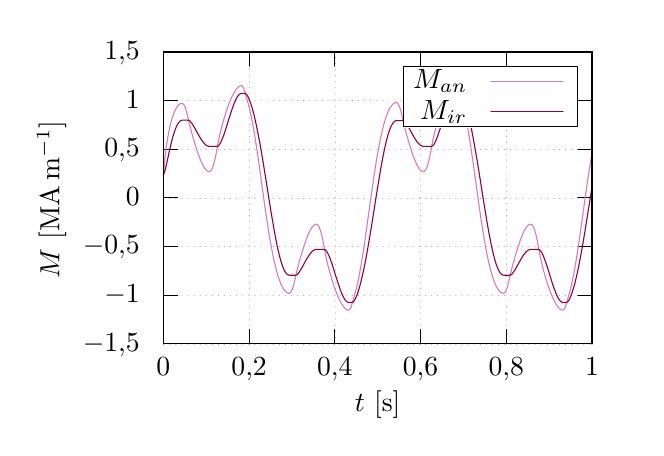
\begin{tikzpicture}[gnuplot]
%% generated with GNUPLOT 5.4p2 (Lua 5.4; terminal rev. Jun 2020, script rev. 114)
%% Fri 23 May 2025 09:04:49 AM -03
\path (0.000,0.000) rectangle (7.500,5.000);
\gpcolor{color=gp lt color axes}
\gpsetlinetype{gp lt axes}
\gpsetdashtype{gp dt axes}
\gpsetlinewidth{0.50}
\draw[gp path] (1.504,0.985)--(6.947,0.985);
\gpcolor{color=gp lt color border}
\gpsetlinetype{gp lt border}
\gpsetdashtype{gp dt solid}
\gpsetlinewidth{1.00}
\draw[gp path] (1.504,0.985)--(1.684,0.985);
\draw[gp path] (6.947,0.985)--(6.767,0.985);
\node[gp node right] at (1.320,0.985) {$-1,5$};
\gpcolor{color=gp lt color axes}
\gpsetlinetype{gp lt axes}
\gpsetdashtype{gp dt axes}
\gpsetlinewidth{0.50}
\draw[gp path] (1.504,1.603)--(6.947,1.603);
\gpcolor{color=gp lt color border}
\gpsetlinetype{gp lt border}
\gpsetdashtype{gp dt solid}
\gpsetlinewidth{1.00}
\draw[gp path] (1.504,1.603)--(1.684,1.603);
\draw[gp path] (6.947,1.603)--(6.767,1.603);
\node[gp node right] at (1.320,1.603) {$-1$};
\gpcolor{color=gp lt color axes}
\gpsetlinetype{gp lt axes}
\gpsetdashtype{gp dt axes}
\gpsetlinewidth{0.50}
\draw[gp path] (1.504,2.220)--(6.947,2.220);
\gpcolor{color=gp lt color border}
\gpsetlinetype{gp lt border}
\gpsetdashtype{gp dt solid}
\gpsetlinewidth{1.00}
\draw[gp path] (1.504,2.220)--(1.684,2.220);
\draw[gp path] (6.947,2.220)--(6.767,2.220);
\node[gp node right] at (1.320,2.220) {$-0,5$};
\gpcolor{color=gp lt color axes}
\gpsetlinetype{gp lt axes}
\gpsetdashtype{gp dt axes}
\gpsetlinewidth{0.50}
\draw[gp path] (1.504,2.838)--(6.947,2.838);
\gpcolor{color=gp lt color border}
\gpsetlinetype{gp lt border}
\gpsetdashtype{gp dt solid}
\gpsetlinewidth{1.00}
\draw[gp path] (1.504,2.838)--(1.684,2.838);
\draw[gp path] (6.947,2.838)--(6.767,2.838);
\node[gp node right] at (1.320,2.838) {$0$};
\gpcolor{color=gp lt color axes}
\gpsetlinetype{gp lt axes}
\gpsetdashtype{gp dt axes}
\gpsetlinewidth{0.50}
\draw[gp path] (1.504,3.456)--(6.947,3.456);
\gpcolor{color=gp lt color border}
\gpsetlinetype{gp lt border}
\gpsetdashtype{gp dt solid}
\gpsetlinewidth{1.00}
\draw[gp path] (1.504,3.456)--(1.684,3.456);
\draw[gp path] (6.947,3.456)--(6.767,3.456);
\node[gp node right] at (1.320,3.456) {$0,5$};
\gpcolor{color=gp lt color axes}
\gpsetlinetype{gp lt axes}
\gpsetdashtype{gp dt axes}
\gpsetlinewidth{0.50}
\draw[gp path] (1.504,4.073)--(4.559,4.073);
\draw[gp path] (6.763,4.073)--(6.947,4.073);
\gpcolor{color=gp lt color border}
\gpsetlinetype{gp lt border}
\gpsetdashtype{gp dt solid}
\gpsetlinewidth{1.00}
\draw[gp path] (1.504,4.073)--(1.684,4.073);
\draw[gp path] (6.947,4.073)--(6.767,4.073);
\node[gp node right] at (1.320,4.073) {$1$};
\gpcolor{color=gp lt color axes}
\gpsetlinetype{gp lt axes}
\gpsetdashtype{gp dt axes}
\gpsetlinewidth{0.50}
\draw[gp path] (1.504,4.691)--(6.947,4.691);
\gpcolor{color=gp lt color border}
\gpsetlinetype{gp lt border}
\gpsetdashtype{gp dt solid}
\gpsetlinewidth{1.00}
\draw[gp path] (1.504,4.691)--(1.684,4.691);
\draw[gp path] (6.947,4.691)--(6.767,4.691);
\node[gp node right] at (1.320,4.691) {$1,5$};
\gpcolor{color=gp lt color axes}
\gpsetlinetype{gp lt axes}
\gpsetdashtype{gp dt axes}
\gpsetlinewidth{0.50}
\draw[gp path] (1.504,0.985)--(1.504,4.691);
\gpcolor{color=gp lt color border}
\gpsetlinetype{gp lt border}
\gpsetdashtype{gp dt solid}
\gpsetlinewidth{1.00}
\draw[gp path] (1.504,0.985)--(1.504,1.165);
\draw[gp path] (1.504,4.691)--(1.504,4.511);
\node[gp node center] at (1.504,0.677) {$0$};
\gpcolor{color=gp lt color axes}
\gpsetlinetype{gp lt axes}
\gpsetdashtype{gp dt axes}
\gpsetlinewidth{0.50}
\draw[gp path] (2.593,0.985)--(2.593,4.691);
\gpcolor{color=gp lt color border}
\gpsetlinetype{gp lt border}
\gpsetdashtype{gp dt solid}
\gpsetlinewidth{1.00}
\draw[gp path] (2.593,0.985)--(2.593,1.165);
\draw[gp path] (2.593,4.691)--(2.593,4.511);
\node[gp node center] at (2.593,0.677) {$0,2$};
\gpcolor{color=gp lt color axes}
\gpsetlinetype{gp lt axes}
\gpsetdashtype{gp dt axes}
\gpsetlinewidth{0.50}
\draw[gp path] (3.681,0.985)--(3.681,4.691);
\gpcolor{color=gp lt color border}
\gpsetlinetype{gp lt border}
\gpsetdashtype{gp dt solid}
\gpsetlinewidth{1.00}
\draw[gp path] (3.681,0.985)--(3.681,1.165);
\draw[gp path] (3.681,4.691)--(3.681,4.511);
\node[gp node center] at (3.681,0.677) {$0,4$};
\gpcolor{color=gp lt color axes}
\gpsetlinetype{gp lt axes}
\gpsetdashtype{gp dt axes}
\gpsetlinewidth{0.50}
\draw[gp path] (4.770,0.985)--(4.770,3.741);
\draw[gp path] (4.770,4.511)--(4.770,4.691);
\gpcolor{color=gp lt color border}
\gpsetlinetype{gp lt border}
\gpsetdashtype{gp dt solid}
\gpsetlinewidth{1.00}
\draw[gp path] (4.770,0.985)--(4.770,1.165);
\draw[gp path] (4.770,4.691)--(4.770,4.511);
\node[gp node center] at (4.770,0.677) {$0,6$};
\gpcolor{color=gp lt color axes}
\gpsetlinetype{gp lt axes}
\gpsetdashtype{gp dt axes}
\gpsetlinewidth{0.50}
\draw[gp path] (5.858,0.985)--(5.858,3.741);
\draw[gp path] (5.858,4.511)--(5.858,4.691);
\gpcolor{color=gp lt color border}
\gpsetlinetype{gp lt border}
\gpsetdashtype{gp dt solid}
\gpsetlinewidth{1.00}
\draw[gp path] (5.858,0.985)--(5.858,1.165);
\draw[gp path] (5.858,4.691)--(5.858,4.511);
\node[gp node center] at (5.858,0.677) {$0,8$};
\gpcolor{color=gp lt color axes}
\gpsetlinetype{gp lt axes}
\gpsetdashtype{gp dt axes}
\gpsetlinewidth{0.50}
\draw[gp path] (6.947,0.985)--(6.947,4.691);
\gpcolor{color=gp lt color border}
\gpsetlinetype{gp lt border}
\gpsetdashtype{gp dt solid}
\gpsetlinewidth{1.00}
\draw[gp path] (6.947,0.985)--(6.947,1.165);
\draw[gp path] (6.947,4.691)--(6.947,4.511);
\node[gp node center] at (6.947,0.677) {$1$};
\draw[gp path] (1.504,4.691)--(1.504,0.985)--(6.947,0.985)--(6.947,4.691)--cycle;
\node[gp node center,rotate=-270] at (0.108,2.838) {$M$ [\si{\mega\ampere\per\meter}]};
\node[gp node center] at (4.225,0.215) {$t$ [\si{\second}]};
\draw[gp path] (4.559,3.741)--(4.559,4.511)--(6.763,4.511)--(6.763,3.741)--cycle;
\gpcolor{rgb color={0.831,0.488,0.735}}
\draw[gp path] (1.504,3.099)--(1.522,3.335)--(1.540,3.485)--(1.559,3.601)--(1.577,3.697)%
  --(1.595,3.777)--(1.613,3.844)--(1.631,3.899)--(1.650,3.944)--(1.668,3.979)--(1.686,4.006)%
  --(1.704,4.025)--(1.722,4.036)--(1.741,4.040)--(1.759,4.030)--(1.777,3.997)--(1.795,3.943)%
  --(1.813,3.871)--(1.832,3.787)--(1.850,3.717)--(1.868,3.651)--(1.886,3.588)--(1.904,3.527)%
  --(1.923,3.469)--(1.941,3.413)--(1.959,3.361)--(1.977,3.314)--(1.996,3.273)--(2.014,3.237)%
  --(2.032,3.209)--(2.050,3.188)--(2.068,3.175)--(2.087,3.171)--(2.105,3.180)--(2.123,3.210)%
  --(2.141,3.261)--(2.159,3.331)--(2.178,3.421)--(2.196,3.525)--(2.214,3.614)--(2.232,3.690)%
  --(2.250,3.761)--(2.269,3.826)--(2.287,3.887)--(2.305,3.944)--(2.323,3.996)--(2.341,4.045)%
  --(2.360,4.090)--(2.378,4.130)--(2.396,4.166)--(2.414,4.196)--(2.432,4.222)--(2.451,4.242)%
  --(2.469,4.256)--(2.487,4.263)--(2.505,4.261)--(2.523,4.233)--(2.542,4.175)--(2.560,4.110)%
  --(2.578,4.047)--(2.596,3.977)--(2.614,3.897)--(2.633,3.807)--(2.651,3.707)--(2.669,3.598)%
  --(2.687,3.481)--(2.705,3.358)--(2.724,3.230)--(2.742,3.099)--(2.760,2.967)--(2.778,2.836)%
  --(2.796,2.707)--(2.815,2.583)--(2.833,2.463)--(2.851,2.351)--(2.869,2.245)--(2.888,2.148)%
  --(2.906,2.059)--(2.924,1.979)--(2.942,1.907)--(2.960,1.844)--(2.979,1.790)--(2.997,1.744)%
  --(3.015,1.706)--(3.033,1.675)--(3.051,1.653)--(3.070,1.637)--(3.088,1.628)--(3.106,1.626)%
  --(3.124,1.642)--(3.142,1.681)--(3.161,1.739)--(3.179,1.816)--(3.197,1.901)--(3.215,1.972)%
  --(3.233,2.038)--(3.252,2.101)--(3.270,2.162)--(3.288,2.220)--(3.306,2.275)--(3.324,2.326)%
  --(3.343,2.372)--(3.361,2.412)--(3.379,2.446)--(3.397,2.472)--(3.415,2.491)--(3.434,2.502)%
  --(3.452,2.504)--(3.470,2.490)--(3.488,2.454)--(3.506,2.399)--(3.525,2.323)--(3.543,2.229)%
  --(3.561,2.126)--(3.579,2.042)--(3.597,1.967)--(3.616,1.899)--(3.634,1.835)--(3.652,1.775)%
  --(3.670,1.719)--(3.688,1.667)--(3.707,1.619)--(3.725,1.576)--(3.743,1.537)--(3.761,1.502)%
  --(3.780,1.473)--(3.798,1.448)--(3.816,1.430)--(3.834,1.418)--(3.852,1.412)--(3.871,1.420)%
  --(3.889,1.455)--(3.907,1.519)--(3.925,1.581)--(3.943,1.646)--(3.962,1.718)--(3.980,1.800)%
  --(3.998,1.893)--(4.016,1.995)--(4.034,2.106)--(4.053,2.225)--(4.071,2.350)--(4.089,2.479)%
  --(4.107,2.610)--(4.125,2.742)--(4.144,2.873)--(4.162,3.000)--(4.180,3.124)--(4.198,3.242)%
  --(4.216,3.353)--(4.235,3.456)--(4.253,3.551)--(4.271,3.638)--(4.289,3.716)--(4.307,3.785)%
  --(4.326,3.846)--(4.344,3.898)--(4.362,3.942)--(4.380,3.979)--(4.398,4.007)--(4.417,4.028)%
  --(4.435,4.042)--(4.453,4.049)--(4.471,4.048)--(4.489,4.026)--(4.508,3.983)--(4.526,3.919)%
  --(4.544,3.838)--(4.562,3.756)--(4.580,3.687)--(4.599,3.622)--(4.617,3.560)--(4.635,3.499)%
  --(4.653,3.442)--(4.671,3.388)--(4.690,3.338)--(4.708,3.294)--(4.726,3.255)--(4.744,3.223)%
  --(4.763,3.198)--(4.781,3.181)--(4.799,3.173)--(4.817,3.174)--(4.835,3.193)--(4.854,3.234)%
  --(4.872,3.294)--(4.890,3.374)--(4.908,3.473)--(4.926,3.572)--(4.945,3.653)--(4.963,3.726)%
  --(4.981,3.794)--(4.999,3.857)--(5.017,3.916)--(5.036,3.970)--(5.054,4.021)--(5.072,4.068)%
  --(5.090,4.110)--(5.108,4.148)--(5.127,4.182)--(5.145,4.210)--(5.163,4.233)--(5.181,4.250)%
  --(5.199,4.260)--(5.218,4.264)--(5.236,4.250)--(5.254,4.208)--(5.272,4.140)--(5.290,4.079)%
  --(5.309,4.013)--(5.327,3.938)--(5.345,3.853)--(5.363,3.758)--(5.381,3.654)--(5.400,3.541)%
  --(5.418,3.420)--(5.436,3.294)--(5.454,3.165)--(5.472,3.033)--(5.491,2.901)--(5.509,2.771)%
  --(5.527,2.644)--(5.545,2.522)--(5.563,2.406)--(5.582,2.297)--(5.600,2.195)--(5.618,2.102)%
  --(5.636,2.018)--(5.655,1.942)--(5.673,1.875)--(5.691,1.816)--(5.709,1.766)--(5.727,1.724)%
  --(5.746,1.690)--(5.764,1.663)--(5.782,1.644)--(5.800,1.632)--(5.818,1.626)--(5.837,1.631)%
  --(5.855,1.659)--(5.873,1.708)--(5.891,1.776)--(5.909,1.861)--(5.928,1.938)--(5.946,2.005)%
  --(5.964,2.070)--(5.982,2.132)--(6.000,2.191)--(6.019,2.248)--(6.037,2.301)--(6.055,2.349)%
  --(6.073,2.393)--(6.091,2.430)--(6.110,2.460)--(6.128,2.483)--(6.146,2.498)--(6.164,2.504)%
  --(6.182,2.499)--(6.201,2.475)--(6.219,2.429)--(6.237,2.363)--(6.255,2.279)--(6.273,2.176)%
  --(6.292,2.083)--(6.310,2.004)--(6.328,1.932)--(6.346,1.866)--(6.364,1.804)--(6.383,1.746)%
  --(6.401,1.692)--(6.419,1.643)--(6.437,1.597)--(6.455,1.556)--(6.474,1.519)--(6.492,1.487)%
  --(6.510,1.460)--(6.528,1.438)--(6.547,1.423)--(6.565,1.414)--(6.583,1.413)--(6.601,1.434)%
  --(6.619,1.484)--(6.638,1.551)--(6.656,1.613)--(6.674,1.681)--(6.692,1.758)--(6.710,1.845)%
  --(6.729,1.943)--(6.747,2.050)--(6.765,2.165)--(6.783,2.287)--(6.801,2.414)--(6.820,2.544)%
  --(6.838,2.676)--(6.856,2.808)--(6.874,2.937)--(6.892,3.063)--(6.911,3.183)--(6.929,3.298)%
  --(6.947,3.405);
\gpcolor{rgb color={0.569,0.000,0.247}}
\draw[gp path] (1.504,3.133)--(1.522,3.174)--(1.540,3.251)--(1.559,3.335)--(1.577,3.419)%
  --(1.595,3.498)--(1.613,3.572)--(1.631,3.637)--(1.650,3.694)--(1.668,3.741)--(1.686,3.777)%
  --(1.704,3.803)--(1.722,3.819)--(1.741,3.825)--(1.759,3.825)--(1.777,3.825)--(1.795,3.825)%
  --(1.813,3.825)--(1.832,3.822)--(1.850,3.806)--(1.868,3.782)--(1.886,3.753)--(1.904,3.722)%
  --(1.923,3.688)--(1.941,3.655)--(1.959,3.622)--(1.977,3.592)--(1.996,3.564)--(2.014,3.540)%
  --(2.032,3.520)--(2.050,3.505)--(2.068,3.496)--(2.087,3.492)--(2.105,3.492)--(2.123,3.492)%
  --(2.141,3.493)--(2.159,3.493)--(2.178,3.493)--(2.196,3.494)--(2.214,3.512)--(2.232,3.543)%
  --(2.250,3.583)--(2.269,3.631)--(2.287,3.684)--(2.305,3.740)--(2.323,3.799)--(2.341,3.857)%
  --(2.360,3.915)--(2.378,3.970)--(2.396,4.021)--(2.414,4.065)--(2.432,4.103)--(2.451,4.133)%
  --(2.469,4.154)--(2.487,4.164)--(2.505,4.166)--(2.523,4.166)--(2.542,4.166)--(2.560,4.154)%
  --(2.578,4.126)--(2.596,4.085)--(2.614,4.035)--(2.633,3.976)--(2.651,3.908)--(2.669,3.832)%
  --(2.687,3.749)--(2.705,3.659)--(2.724,3.563)--(2.742,3.461)--(2.760,3.355)--(2.778,3.245)%
  --(2.796,3.132)--(2.815,3.017)--(2.833,2.901)--(2.851,2.786)--(2.869,2.673)--(2.888,2.562)%
  --(2.906,2.456)--(2.924,2.356)--(2.942,2.263)--(2.960,2.178)--(2.979,2.101)--(2.997,2.035)%
  --(3.015,1.978)--(3.033,1.932)--(3.051,1.898)--(3.070,1.873)--(3.088,1.860)--(3.106,1.856)%
  --(3.124,1.856)--(3.142,1.856)--(3.161,1.856)--(3.179,1.856)--(3.197,1.860)--(3.215,1.877)%
  --(3.233,1.902)--(3.252,1.932)--(3.270,1.963)--(3.288,1.997)--(3.306,2.030)--(3.324,2.062)%
  --(3.343,2.092)--(3.361,2.119)--(3.379,2.142)--(3.397,2.161)--(3.415,2.174)--(3.434,2.182)%
  --(3.452,2.184)--(3.470,2.184)--(3.488,2.184)--(3.506,2.184)--(3.525,2.184)--(3.543,2.184)%
  --(3.561,2.179)--(3.579,2.158)--(3.597,2.124)--(3.616,2.082)--(3.634,2.033)--(3.652,1.979)%
  --(3.670,1.921)--(3.688,1.863)--(3.707,1.804)--(3.725,1.747)--(3.743,1.693)--(3.761,1.644)%
  --(3.780,1.600)--(3.798,1.565)--(3.816,1.537)--(3.834,1.519)--(3.852,1.511)--(3.871,1.510)%
  --(3.889,1.510)--(3.907,1.511)--(3.925,1.528)--(3.943,1.559)--(3.962,1.602)--(3.980,1.655)%
  --(3.998,1.717)--(4.016,1.786)--(4.034,1.864)--(4.053,1.949)--(4.071,2.041)--(4.089,2.138)%
  --(4.107,2.241)--(4.125,2.348)--(4.144,2.459)--(4.162,2.573)--(4.180,2.688)--(4.198,2.804)%
  --(4.216,2.919)--(4.235,3.031)--(4.253,3.141)--(4.271,3.245)--(4.289,3.344)--(4.307,3.435)%
  --(4.326,3.518)--(4.344,3.592)--(4.362,3.657)--(4.380,3.710)--(4.398,3.753)--(4.417,3.785)%
  --(4.435,3.807)--(4.453,3.818)--(4.471,3.820)--(4.489,3.820)--(4.508,3.820)--(4.526,3.820)%
  --(4.544,3.820)--(4.562,3.813)--(4.580,3.793)--(4.599,3.767)--(4.617,3.737)--(4.635,3.704)%
  --(4.653,3.671)--(4.671,3.638)--(4.690,3.606)--(4.708,3.577)--(4.726,3.551)--(4.744,3.529)%
  --(4.763,3.511)--(4.781,3.499)--(4.799,3.493)--(4.817,3.492)--(4.835,3.492)--(4.854,3.492)%
  --(4.872,3.492)--(4.890,3.492)--(4.908,3.492)--(4.926,3.501)--(4.945,3.526)--(4.963,3.562)%
  --(4.981,3.606)--(4.999,3.657)--(5.017,3.711)--(5.036,3.769)--(5.054,3.828)--(5.072,3.887)%
  --(5.090,3.943)--(5.108,3.996)--(5.127,4.044)--(5.145,4.085)--(5.163,4.119)--(5.181,4.144)%
  --(5.199,4.160)--(5.218,4.166)--(5.236,4.166)--(5.254,4.166)--(5.272,4.163)--(5.290,4.141)%
  --(5.309,4.107)--(5.327,4.061)--(5.345,4.007)--(5.363,3.943)--(5.381,3.871)--(5.400,3.791)%
  --(5.418,3.705)--(5.436,3.611)--(5.454,3.513)--(5.472,3.408)--(5.491,3.300)--(5.509,3.188)%
  --(5.527,3.074)--(5.545,2.959)--(5.563,2.843)--(5.582,2.729)--(5.600,2.617)--(5.618,2.509)%
  --(5.636,2.406)--(5.655,2.309)--(5.673,2.219)--(5.691,2.138)--(5.709,2.067)--(5.727,2.005)%
  --(5.746,1.954)--(5.764,1.914)--(5.782,1.884)--(5.800,1.865)--(5.818,1.857)--(5.837,1.856)%
  --(5.855,1.856)--(5.873,1.856)--(5.891,1.856)--(5.909,1.856)--(5.928,1.868)--(5.946,1.889)%
  --(5.964,1.917)--(5.982,1.947)--(6.000,1.980)--(6.019,2.013)--(6.037,2.046)--(6.055,2.077)%
  --(6.073,2.106)--(6.091,2.131)--(6.110,2.152)--(6.128,2.168)--(6.146,2.179)--(6.164,2.184)%
  --(6.182,2.184)--(6.201,2.184)--(6.219,2.184)--(6.237,2.184)--(6.255,2.184)--(6.273,2.184)%
  --(6.292,2.170)--(6.310,2.142)--(6.328,2.104)--(6.346,2.058)--(6.364,2.006)--(6.383,1.950)%
  --(6.401,1.892)--(6.419,1.833)--(6.437,1.775)--(6.455,1.719)--(6.474,1.668)--(6.492,1.621)%
  --(6.510,1.582)--(6.528,1.550)--(6.547,1.527)--(6.565,1.513)--(6.583,1.510)--(6.601,1.510)%
  --(6.619,1.510)--(6.638,1.517)--(6.656,1.542)--(6.674,1.580)--(6.692,1.627)--(6.710,1.685)%
  --(6.729,1.750)--(6.747,1.824)--(6.765,1.906)--(6.783,1.994)--(6.801,2.089)--(6.820,2.189)%
  --(6.838,2.294)--(6.856,2.404)--(6.874,2.516)--(6.892,2.630)--(6.911,2.746)--(6.929,2.861)%
  --(6.947,2.975);
\gpfill{color=gpbgfillcolor} (4.559,3.741)--(6.763,3.741)--(6.763,4.511)--(4.559,4.511)--cycle;
\gpcolor{color=gp lt color border}
\draw[gp path] (4.559,3.741)--(4.559,4.511)--(6.763,4.511)--(6.763,3.741)--cycle;
\node[gp node right] at (5.479,4.318) {\phantom{M}$M_{an}$};
\gpcolor{rgb color={0.831,0.488,0.735}}
\draw[gp path] (5.663,4.318)--(6.579,4.318);
\gpcolor{color=gp lt color border}
\node[gp node right] at (5.479,3.933) {\phantom{M}$M_{ir}$};
\gpcolor{rgb color={0.569,0.000,0.247}}
\draw[gp path] (5.663,3.933)--(6.579,3.933);
\gpcolor{color=gp lt color border}
\draw[gp path] (1.504,4.691)--(1.504,0.985)--(6.947,0.985)--(6.947,4.691)--cycle;
%% coordinates of the plot area
\gpdefrectangularnode{gp plot 1}{\pgfpoint{1.504cm}{0.985cm}}{\pgfpoint{6.947cm}{4.691cm}}
\end{tikzpicture}
%% gnuplot variables

    \vspace{-1cm}
    \caption{HHHHHHHHHHHHHHH}
  \end{minipage}%
\end{figure}

\newpage

\begin{figure}[!h]
  \begin{minipage}{.49\linewidth}
    \centering
    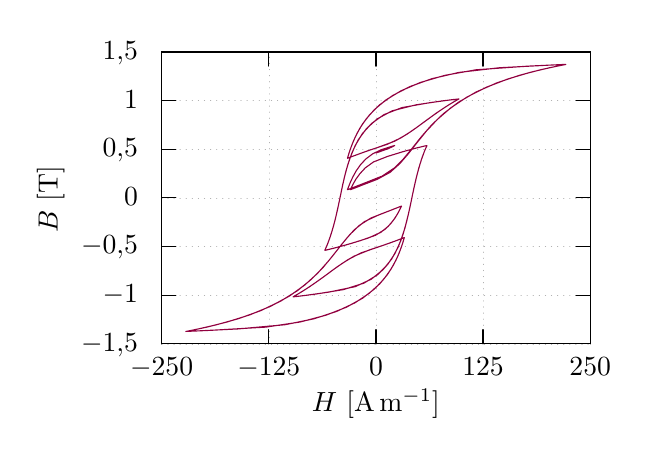
\begin{tikzpicture}[gnuplot]
%% generated with GNUPLOT 5.4p2 (Lua 5.4; terminal rev. Jun 2020, script rev. 114)
%% Fri 23 May 2025 09:04:29 AM -03
\path (0.000,0.000) rectangle (7.500,5.000);
\gpcolor{color=gp lt color axes}
\gpsetlinetype{gp lt axes}
\gpsetdashtype{gp dt axes}
\gpsetlinewidth{0.50}
\draw[gp path] (1.504,0.985)--(6.947,0.985);
\gpcolor{color=gp lt color border}
\gpsetlinetype{gp lt border}
\gpsetdashtype{gp dt solid}
\gpsetlinewidth{1.00}
\draw[gp path] (1.504,0.985)--(1.684,0.985);
\draw[gp path] (6.947,0.985)--(6.767,0.985);
\node[gp node right] at (1.320,0.985) {$-1,5$};
\gpcolor{color=gp lt color axes}
\gpsetlinetype{gp lt axes}
\gpsetdashtype{gp dt axes}
\gpsetlinewidth{0.50}
\draw[gp path] (1.504,1.603)--(6.947,1.603);
\gpcolor{color=gp lt color border}
\gpsetlinetype{gp lt border}
\gpsetdashtype{gp dt solid}
\gpsetlinewidth{1.00}
\draw[gp path] (1.504,1.603)--(1.684,1.603);
\draw[gp path] (6.947,1.603)--(6.767,1.603);
\node[gp node right] at (1.320,1.603) {$-1$};
\gpcolor{color=gp lt color axes}
\gpsetlinetype{gp lt axes}
\gpsetdashtype{gp dt axes}
\gpsetlinewidth{0.50}
\draw[gp path] (1.504,2.220)--(6.947,2.220);
\gpcolor{color=gp lt color border}
\gpsetlinetype{gp lt border}
\gpsetdashtype{gp dt solid}
\gpsetlinewidth{1.00}
\draw[gp path] (1.504,2.220)--(1.684,2.220);
\draw[gp path] (6.947,2.220)--(6.767,2.220);
\node[gp node right] at (1.320,2.220) {$-0,5$};
\gpcolor{color=gp lt color axes}
\gpsetlinetype{gp lt axes}
\gpsetdashtype{gp dt axes}
\gpsetlinewidth{0.50}
\draw[gp path] (1.504,2.838)--(6.947,2.838);
\gpcolor{color=gp lt color border}
\gpsetlinetype{gp lt border}
\gpsetdashtype{gp dt solid}
\gpsetlinewidth{1.00}
\draw[gp path] (1.504,2.838)--(1.684,2.838);
\draw[gp path] (6.947,2.838)--(6.767,2.838);
\node[gp node right] at (1.320,2.838) {$0$};
\gpcolor{color=gp lt color axes}
\gpsetlinetype{gp lt axes}
\gpsetdashtype{gp dt axes}
\gpsetlinewidth{0.50}
\draw[gp path] (1.504,3.456)--(6.947,3.456);
\gpcolor{color=gp lt color border}
\gpsetlinetype{gp lt border}
\gpsetdashtype{gp dt solid}
\gpsetlinewidth{1.00}
\draw[gp path] (1.504,3.456)--(1.684,3.456);
\draw[gp path] (6.947,3.456)--(6.767,3.456);
\node[gp node right] at (1.320,3.456) {$0,5$};
\gpcolor{color=gp lt color axes}
\gpsetlinetype{gp lt axes}
\gpsetdashtype{gp dt axes}
\gpsetlinewidth{0.50}
\draw[gp path] (1.504,4.073)--(6.947,4.073);
\gpcolor{color=gp lt color border}
\gpsetlinetype{gp lt border}
\gpsetdashtype{gp dt solid}
\gpsetlinewidth{1.00}
\draw[gp path] (1.504,4.073)--(1.684,4.073);
\draw[gp path] (6.947,4.073)--(6.767,4.073);
\node[gp node right] at (1.320,4.073) {$1$};
\gpcolor{color=gp lt color axes}
\gpsetlinetype{gp lt axes}
\gpsetdashtype{gp dt axes}
\gpsetlinewidth{0.50}
\draw[gp path] (1.504,4.691)--(6.947,4.691);
\gpcolor{color=gp lt color border}
\gpsetlinetype{gp lt border}
\gpsetdashtype{gp dt solid}
\gpsetlinewidth{1.00}
\draw[gp path] (1.504,4.691)--(1.684,4.691);
\draw[gp path] (6.947,4.691)--(6.767,4.691);
\node[gp node right] at (1.320,4.691) {$1,5$};
\gpcolor{color=gp lt color axes}
\gpsetlinetype{gp lt axes}
\gpsetdashtype{gp dt axes}
\gpsetlinewidth{0.50}
\draw[gp path] (1.504,0.985)--(1.504,4.691);
\gpcolor{color=gp lt color border}
\gpsetlinetype{gp lt border}
\gpsetdashtype{gp dt solid}
\gpsetlinewidth{1.00}
\draw[gp path] (1.504,0.985)--(1.504,1.165);
\draw[gp path] (1.504,4.691)--(1.504,4.511);
\node[gp node center] at (1.504,0.677) {$-250$};
\gpcolor{color=gp lt color axes}
\gpsetlinetype{gp lt axes}
\gpsetdashtype{gp dt axes}
\gpsetlinewidth{0.50}
\draw[gp path] (2.865,0.985)--(2.865,4.691);
\gpcolor{color=gp lt color border}
\gpsetlinetype{gp lt border}
\gpsetdashtype{gp dt solid}
\gpsetlinewidth{1.00}
\draw[gp path] (2.865,0.985)--(2.865,1.165);
\draw[gp path] (2.865,4.691)--(2.865,4.511);
\node[gp node center] at (2.865,0.677) {$-125$};
\gpcolor{color=gp lt color axes}
\gpsetlinetype{gp lt axes}
\gpsetdashtype{gp dt axes}
\gpsetlinewidth{0.50}
\draw[gp path] (4.226,0.985)--(4.226,4.691);
\gpcolor{color=gp lt color border}
\gpsetlinetype{gp lt border}
\gpsetdashtype{gp dt solid}
\gpsetlinewidth{1.00}
\draw[gp path] (4.226,0.985)--(4.226,1.165);
\draw[gp path] (4.226,4.691)--(4.226,4.511);
\node[gp node center] at (4.226,0.677) {$0$};
\gpcolor{color=gp lt color axes}
\gpsetlinetype{gp lt axes}
\gpsetdashtype{gp dt axes}
\gpsetlinewidth{0.50}
\draw[gp path] (5.586,0.985)--(5.586,4.691);
\gpcolor{color=gp lt color border}
\gpsetlinetype{gp lt border}
\gpsetdashtype{gp dt solid}
\gpsetlinewidth{1.00}
\draw[gp path] (5.586,0.985)--(5.586,1.165);
\draw[gp path] (5.586,4.691)--(5.586,4.511);
\node[gp node center] at (5.586,0.677) {$125$};
\gpcolor{color=gp lt color axes}
\gpsetlinetype{gp lt axes}
\gpsetdashtype{gp dt axes}
\gpsetlinewidth{0.50}
\draw[gp path] (6.947,0.985)--(6.947,4.691);
\gpcolor{color=gp lt color border}
\gpsetlinetype{gp lt border}
\gpsetdashtype{gp dt solid}
\gpsetlinewidth{1.00}
\draw[gp path] (6.947,0.985)--(6.947,1.165);
\draw[gp path] (6.947,4.691)--(6.947,4.511);
\node[gp node center] at (6.947,0.677) {$250$};
\draw[gp path] (1.504,4.691)--(1.504,0.985)--(6.947,0.985)--(6.947,4.691)--cycle;
\node[gp node center,rotate=-270] at (0.108,2.838) {$B$ [\si{\tesla}]};
\node[gp node center] at (4.225,0.215) {$H$ [\si{\ampere\per\meter}]};
\gpcolor{rgb color={0.569,0.000,0.247}}
\draw[gp path] (4.226,3.408)--(4.387,3.465)--(4.453,3.497)--(4.464,3.504)--(4.409,3.487)%
  --(4.293,3.450)--(4.183,3.397)--(4.096,3.331)--(4.028,3.257)--(3.975,3.181)--(3.935,3.109)%
  --(3.904,3.044)--(3.883,2.992)--(3.869,2.957)--(3.864,2.942)--(3.884,2.949)--(3.965,2.981)%
  --(4.108,3.037)--(4.307,3.116)--(4.457,3.216)--(4.576,3.335)--(4.686,3.468)--(4.800,3.612)%
  --(4.929,3.760)--(5.083,3.908)--(5.271,4.051)--(5.496,4.182)--(5.759,4.298)--(6.044,4.394)%
  --(6.319,4.466)--(6.535,4.513)--(6.637,4.533)--(6.442,4.525)--(5.792,4.491)--(5.281,4.432)%
  --(4.936,4.352)--(4.660,4.253)--(4.442,4.141)--(4.274,4.021)--(4.148,3.897)--(4.055,3.776)%
  --(3.988,3.662)--(3.940,3.560)--(3.907,3.474)--(3.884,3.408)--(3.871,3.364)--(3.865,3.343)%
  --(3.876,3.346)--(3.942,3.371)--(4.067,3.417)--(4.252,3.480)--(4.464,3.558)--(4.617,3.645)%
  --(4.748,3.736)--(4.871,3.827)--(4.988,3.912)--(5.097,3.985)--(5.189,4.043)--(5.253,4.080)%
  --(5.280,4.095)--(5.189,4.085)--(4.913,4.048)--(4.556,3.985)--(4.328,3.896)--(4.170,3.783)%
  --(4.051,3.651)--(3.962,3.502)--(3.895,3.342)--(3.844,3.175)--(3.804,3.007)--(3.770,2.843)%
  --(3.738,2.689)--(3.705,2.549)--(3.671,2.427)--(3.639,2.327)--(3.611,2.251)--(3.589,2.200)%
  --(3.578,2.175)--(3.588,2.174)--(3.679,2.196)--(3.836,2.238)--(4.027,2.295)--(4.220,2.363)%
  --(4.339,2.438)--(4.415,2.513)--(4.469,2.584)--(4.506,2.646)--(4.532,2.695)--(4.546,2.725)%
  --(4.551,2.734)--(4.516,2.721)--(4.419,2.683)--(4.261,2.622)--(4.080,2.537)--(3.950,2.432)%
  --(3.840,2.309)--(3.732,2.173)--(3.616,2.028)--(3.483,1.879)--(3.322,1.732)--(3.126,1.591)%
  --(2.891,1.463)--(2.622,1.352)--(2.335,1.262)--(2.070,1.195)--(1.878,1.155)--(1.811,1.142)%
  --(2.143,1.157)--(2.827,1.197)--(3.264,1.262)--(3.590,1.348)--(3.851,1.450)--(4.056,1.564)%
  --(4.212,1.686)--(4.329,1.810)--(4.415,1.930)--(4.477,2.041)--(4.521,2.139)--(4.551,2.220)%
  --(4.571,2.281)--(4.582,2.319)--(4.586,2.334)--(4.564,2.326)--(4.483,2.295)--(4.344,2.245)%
  --(4.142,2.177)--(3.945,2.097)--(3.800,2.008)--(3.671,1.917)--(3.550,1.827)--(3.434,1.745)%
  --(3.329,1.675)--(3.243,1.622)--(3.187,1.590)--(3.174,1.581)--(3.317,1.598)--(3.625,1.641)%
  --(3.963,1.711)--(4.167,1.806)--(4.314,1.924)--(4.425,2.061)--(4.508,2.213)--(4.570,2.375)%
  --(4.617,2.543)--(4.656,2.711)--(4.689,2.872)--(4.722,3.024)--(4.755,3.159)--(4.788,3.276)%
  --(4.819,3.370)--(4.846,3.440)--(4.865,3.484)--(4.874,3.503)--(4.848,3.498)--(4.737,3.471)%
  --(4.569,3.425)--(4.374,3.365)--(4.195,3.295)--(4.090,3.219)--(4.021,3.144)--(3.971,3.075)%
  --(3.937,3.016)--(3.915,2.972)--(3.902,2.947)--(3.903,2.943)--(3.954,2.962)--(4.065,3.006)%
  --(4.240,3.073)--(4.406,3.163)--(4.529,3.273)--(4.638,3.400)--(4.747,3.539)--(4.866,3.686)%
  --(5.005,3.834)--(5.174,3.980)--(5.380,4.118)--(5.624,4.242)--(5.900,4.348)--(6.186,4.433)%
  --(6.438,4.493)--(6.603,4.526)--(6.614,4.533)--(6.150,4.511)--(5.496,4.465)--(5.098,4.394)%
  --(4.790,4.304)--(4.544,4.198)--(4.352,4.082)--(4.206,3.959)--(4.098,3.836)--(4.019,3.718)%
  --(3.962,3.609)--(3.922,3.515)--(3.894,3.439)--(3.877,3.383)--(3.867,3.351)--(3.865,3.341)%
  --(3.902,3.356)--(3.997,3.391)--(4.152,3.447)--(4.368,3.518)--(4.545,3.601)--(4.684,3.690)%
  --(4.811,3.782)--(4.931,3.870)--(5.044,3.950)--(5.145,4.016)--(5.225,4.064)--(5.272,4.091)%
  --(5.261,4.093)--(5.069,4.070)--(4.734,4.020)--(4.429,3.943)--(4.243,3.842)--(4.107,3.720)%
  --(4.003,3.578)--(3.926,3.423)--(3.868,3.259)--(3.823,3.091)--(3.787,2.924)--(3.754,2.765)%
  --(3.721,2.617)--(3.688,2.485)--(3.655,2.374)--(3.624,2.286)--(3.599,2.223)--(3.582,2.185)%
  --(3.577,2.172)--(3.623,2.183)--(3.751,2.215)--(3.929,2.265)--(4.128,2.328)--(4.287,2.400)%
  --(4.381,2.476)--(4.444,2.550)--(4.489,2.617)--(4.521,2.673)--(4.540,2.712)--(4.550,2.733)%
  --(4.541,2.731)--(4.475,2.705)--(4.348,2.655)--(4.161,2.582)--(4.012,2.487)--(3.894,2.372)%
  --(3.786,2.242)--(3.676,2.101)--(3.553,1.953)--(3.407,1.805)--(3.229,1.660)--(3.014,1.526)%
  --(2.760,1.405)--(2.479,1.304)--(2.197,1.226)--(1.961,1.172)--(1.827,1.145)--(1.905,1.146)%
  --(2.475,1.174)--(3.068,1.227)--(3.437,1.302)--(3.728,1.397)--(3.960,1.506)--(4.139,1.625)%
  --(4.275,1.748)--(4.376,1.870)--(4.449,1.987)--(4.501,2.092)--(4.537,2.182)--(4.562,2.253)%
  --(4.577,2.303)--(4.585,2.330)--(4.582,2.333)--(4.531,2.313)--(4.421,2.272)--(4.251,2.213)%
  --(4.032,2.138)--(3.869,2.053)--(3.734,1.963)--(3.610,1.871)--(3.491,1.785)--(3.380,1.708)%
  --(3.283,1.646)--(3.211,1.603)--(3.174,1.582)--(3.220,1.586)--(3.457,1.616)--(3.812,1.673)%
  --(4.075,1.756)--(4.246,1.862)--(4.373,1.990)--(4.469,2.135)--(4.541,2.293)--(4.595,2.459)%
  --(4.637,2.627)--(4.673,2.793)--(4.705,2.950)--(4.738,3.094)--(4.771,3.220)--(4.804,3.326)%
  --(4.834,3.408);
\gpcolor{color=gp lt color border}
\draw[gp path] (1.504,4.691)--(1.504,0.985)--(6.947,0.985)--(6.947,4.691)--cycle;
%% coordinates of the plot area
\gpdefrectangularnode{gp plot 1}{\pgfpoint{1.504cm}{0.985cm}}{\pgfpoint{6.947cm}{4.691cm}}
\end{tikzpicture}
%% gnuplot variables

    \vspace{-1cm}
    \caption{uma caption}
  \end{minipage}%
  \begin{minipage}{.49\linewidth}
    \centering
    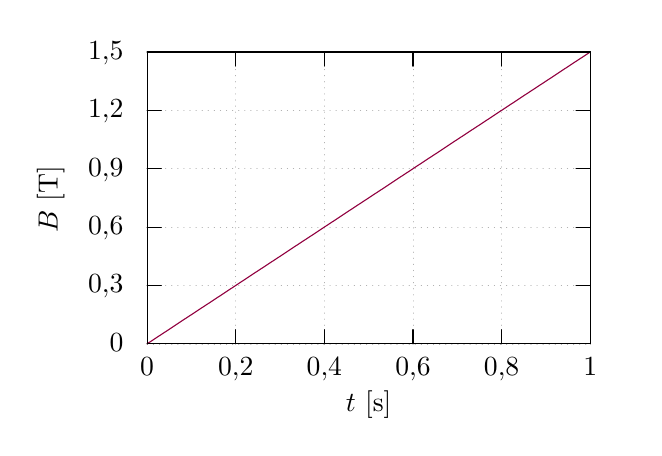
\begin{tikzpicture}[gnuplot]
%% generated with GNUPLOT 5.4p2 (Lua 5.4; terminal rev. Jun 2020, script rev. 114)
%% Fri 23 May 2025 09:06:32 AM -03
\path (0.000,0.000) rectangle (7.500,5.000);
\gpcolor{color=gp lt color axes}
\gpsetlinetype{gp lt axes}
\gpsetdashtype{gp dt axes}
\gpsetlinewidth{0.50}
\draw[gp path] (1.320,0.985)--(6.947,0.985);
\gpcolor{color=gp lt color border}
\gpsetlinetype{gp lt border}
\gpsetdashtype{gp dt solid}
\gpsetlinewidth{1.00}
\draw[gp path] (1.320,0.985)--(1.500,0.985);
\draw[gp path] (6.947,0.985)--(6.767,0.985);
\node[gp node right] at (1.136,0.985) {$0$};
\gpcolor{color=gp lt color axes}
\gpsetlinetype{gp lt axes}
\gpsetdashtype{gp dt axes}
\gpsetlinewidth{0.50}
\draw[gp path] (1.320,1.726)--(6.947,1.726);
\gpcolor{color=gp lt color border}
\gpsetlinetype{gp lt border}
\gpsetdashtype{gp dt solid}
\gpsetlinewidth{1.00}
\draw[gp path] (1.320,1.726)--(1.500,1.726);
\draw[gp path] (6.947,1.726)--(6.767,1.726);
\node[gp node right] at (1.136,1.726) {$0,3$};
\gpcolor{color=gp lt color axes}
\gpsetlinetype{gp lt axes}
\gpsetdashtype{gp dt axes}
\gpsetlinewidth{0.50}
\draw[gp path] (1.320,2.467)--(6.947,2.467);
\gpcolor{color=gp lt color border}
\gpsetlinetype{gp lt border}
\gpsetdashtype{gp dt solid}
\gpsetlinewidth{1.00}
\draw[gp path] (1.320,2.467)--(1.500,2.467);
\draw[gp path] (6.947,2.467)--(6.767,2.467);
\node[gp node right] at (1.136,2.467) {$0,6$};
\gpcolor{color=gp lt color axes}
\gpsetlinetype{gp lt axes}
\gpsetdashtype{gp dt axes}
\gpsetlinewidth{0.50}
\draw[gp path] (1.320,3.209)--(6.947,3.209);
\gpcolor{color=gp lt color border}
\gpsetlinetype{gp lt border}
\gpsetdashtype{gp dt solid}
\gpsetlinewidth{1.00}
\draw[gp path] (1.320,3.209)--(1.500,3.209);
\draw[gp path] (6.947,3.209)--(6.767,3.209);
\node[gp node right] at (1.136,3.209) {$0,9$};
\gpcolor{color=gp lt color axes}
\gpsetlinetype{gp lt axes}
\gpsetdashtype{gp dt axes}
\gpsetlinewidth{0.50}
\draw[gp path] (1.320,3.950)--(6.947,3.950);
\gpcolor{color=gp lt color border}
\gpsetlinetype{gp lt border}
\gpsetdashtype{gp dt solid}
\gpsetlinewidth{1.00}
\draw[gp path] (1.320,3.950)--(1.500,3.950);
\draw[gp path] (6.947,3.950)--(6.767,3.950);
\node[gp node right] at (1.136,3.950) {$1,2$};
\gpcolor{color=gp lt color axes}
\gpsetlinetype{gp lt axes}
\gpsetdashtype{gp dt axes}
\gpsetlinewidth{0.50}
\draw[gp path] (1.320,4.691)--(6.947,4.691);
\gpcolor{color=gp lt color border}
\gpsetlinetype{gp lt border}
\gpsetdashtype{gp dt solid}
\gpsetlinewidth{1.00}
\draw[gp path] (1.320,4.691)--(1.500,4.691);
\draw[gp path] (6.947,4.691)--(6.767,4.691);
\node[gp node right] at (1.136,4.691) {$1,5$};
\gpcolor{color=gp lt color axes}
\gpsetlinetype{gp lt axes}
\gpsetdashtype{gp dt axes}
\gpsetlinewidth{0.50}
\draw[gp path] (1.320,0.985)--(1.320,4.691);
\gpcolor{color=gp lt color border}
\gpsetlinetype{gp lt border}
\gpsetdashtype{gp dt solid}
\gpsetlinewidth{1.00}
\draw[gp path] (1.320,0.985)--(1.320,1.165);
\draw[gp path] (1.320,4.691)--(1.320,4.511);
\node[gp node center] at (1.320,0.677) {$0$};
\gpcolor{color=gp lt color axes}
\gpsetlinetype{gp lt axes}
\gpsetdashtype{gp dt axes}
\gpsetlinewidth{0.50}
\draw[gp path] (2.445,0.985)--(2.445,4.691);
\gpcolor{color=gp lt color border}
\gpsetlinetype{gp lt border}
\gpsetdashtype{gp dt solid}
\gpsetlinewidth{1.00}
\draw[gp path] (2.445,0.985)--(2.445,1.165);
\draw[gp path] (2.445,4.691)--(2.445,4.511);
\node[gp node center] at (2.445,0.677) {$0,2$};
\gpcolor{color=gp lt color axes}
\gpsetlinetype{gp lt axes}
\gpsetdashtype{gp dt axes}
\gpsetlinewidth{0.50}
\draw[gp path] (3.571,0.985)--(3.571,4.691);
\gpcolor{color=gp lt color border}
\gpsetlinetype{gp lt border}
\gpsetdashtype{gp dt solid}
\gpsetlinewidth{1.00}
\draw[gp path] (3.571,0.985)--(3.571,1.165);
\draw[gp path] (3.571,4.691)--(3.571,4.511);
\node[gp node center] at (3.571,0.677) {$0,4$};
\gpcolor{color=gp lt color axes}
\gpsetlinetype{gp lt axes}
\gpsetdashtype{gp dt axes}
\gpsetlinewidth{0.50}
\draw[gp path] (4.696,0.985)--(4.696,4.691);
\gpcolor{color=gp lt color border}
\gpsetlinetype{gp lt border}
\gpsetdashtype{gp dt solid}
\gpsetlinewidth{1.00}
\draw[gp path] (4.696,0.985)--(4.696,1.165);
\draw[gp path] (4.696,4.691)--(4.696,4.511);
\node[gp node center] at (4.696,0.677) {$0,6$};
\gpcolor{color=gp lt color axes}
\gpsetlinetype{gp lt axes}
\gpsetdashtype{gp dt axes}
\gpsetlinewidth{0.50}
\draw[gp path] (5.822,0.985)--(5.822,4.691);
\gpcolor{color=gp lt color border}
\gpsetlinetype{gp lt border}
\gpsetdashtype{gp dt solid}
\gpsetlinewidth{1.00}
\draw[gp path] (5.822,0.985)--(5.822,1.165);
\draw[gp path] (5.822,4.691)--(5.822,4.511);
\node[gp node center] at (5.822,0.677) {$0,8$};
\gpcolor{color=gp lt color axes}
\gpsetlinetype{gp lt axes}
\gpsetdashtype{gp dt axes}
\gpsetlinewidth{0.50}
\draw[gp path] (6.947,0.985)--(6.947,4.691);
\gpcolor{color=gp lt color border}
\gpsetlinetype{gp lt border}
\gpsetdashtype{gp dt solid}
\gpsetlinewidth{1.00}
\draw[gp path] (6.947,0.985)--(6.947,1.165);
\draw[gp path] (6.947,4.691)--(6.947,4.511);
\node[gp node center] at (6.947,0.677) {$1$};
\draw[gp path] (1.320,4.691)--(1.320,0.985)--(6.947,0.985)--(6.947,4.691)--cycle;
\node[gp node center,rotate=-270] at (0.108,2.838) {$B$ [\si{\tesla}]};
\node[gp node center] at (4.133,0.215) {$t$ [\si{\second}]};
\gpcolor{rgb color={0.569,0.000,0.247}}
\draw[gp path] (1.320,0.985)--(1.435,1.061)--(1.550,1.136)--(1.665,1.212)--(1.779,1.288)%
  --(1.894,1.363)--(2.009,1.439)--(2.124,1.514)--(2.239,1.590)--(2.354,1.666)--(2.468,1.741)%
  --(2.583,1.817)--(2.698,1.893)--(2.813,1.968)--(2.928,2.044)--(3.043,2.119)--(3.157,2.195)%
  --(3.272,2.271)--(3.387,2.346)--(3.502,2.422)--(3.617,2.498)--(3.732,2.573)--(3.846,2.649)%
  --(3.961,2.725)--(4.076,2.800)--(4.191,2.876)--(4.306,2.951)--(4.421,3.027)--(4.535,3.103)%
  --(4.650,3.178)--(4.765,3.254)--(4.880,3.330)--(4.995,3.405)--(5.110,3.481)--(5.224,3.557)%
  --(5.339,3.632)--(5.454,3.708)--(5.569,3.783)--(5.684,3.859)--(5.799,3.935)--(5.913,4.010)%
  --(6.028,4.086)--(6.143,4.162)--(6.258,4.237)--(6.373,4.313)--(6.488,4.388)--(6.602,4.464)%
  --(6.717,4.540)--(6.832,4.615)--(6.947,4.691);
\gpcolor{color=gp lt color border}
\draw[gp path] (1.320,4.691)--(1.320,0.985)--(6.947,0.985)--(6.947,4.691)--cycle;
%% coordinates of the plot area
\gpdefrectangularnode{gp plot 1}{\pgfpoint{1.320cm}{0.985cm}}{\pgfpoint{6.947cm}{4.691cm}}
\end{tikzpicture}
%% gnuplot variables

    \vspace{-1cm}
    \caption{HHHHHHHHHHHHHHH}
  \end{minipage}
  \begin{minipage}{.49\linewidth}
    \centering
    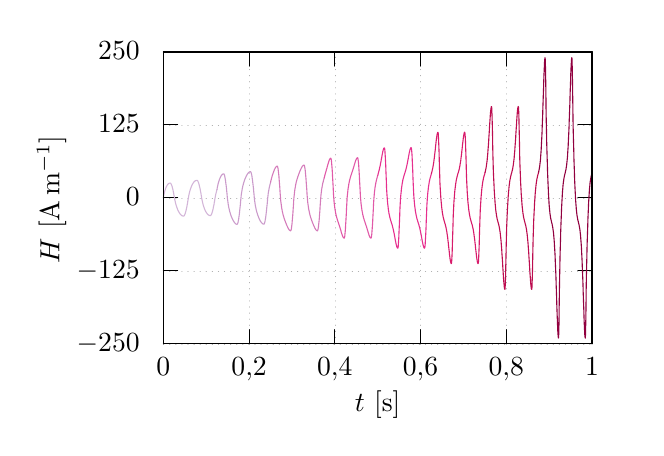
\begin{tikzpicture}[gnuplot]
%% generated with GNUPLOT 5.4p2 (Lua 5.4; terminal rev. Jun 2020, script rev. 114)
%% Fri 23 May 2025 09:05:47 AM -03
\path (0.000,0.000) rectangle (7.500,5.000);
\gpcolor{color=gp lt color axes}
\gpsetlinetype{gp lt axes}
\gpsetdashtype{gp dt axes}
\gpsetlinewidth{0.50}
\draw[gp path] (1.504,0.985)--(6.947,0.985);
\gpcolor{color=gp lt color border}
\gpsetlinetype{gp lt border}
\gpsetdashtype{gp dt solid}
\gpsetlinewidth{1.00}
\draw[gp path] (1.504,0.985)--(1.684,0.985);
\draw[gp path] (6.947,0.985)--(6.767,0.985);
\node[gp node right] at (1.320,0.985) {$-250$};
\gpcolor{color=gp lt color axes}
\gpsetlinetype{gp lt axes}
\gpsetdashtype{gp dt axes}
\gpsetlinewidth{0.50}
\draw[gp path] (1.504,1.912)--(6.947,1.912);
\gpcolor{color=gp lt color border}
\gpsetlinetype{gp lt border}
\gpsetdashtype{gp dt solid}
\gpsetlinewidth{1.00}
\draw[gp path] (1.504,1.912)--(1.684,1.912);
\draw[gp path] (6.947,1.912)--(6.767,1.912);
\node[gp node right] at (1.320,1.912) {$-125$};
\gpcolor{color=gp lt color axes}
\gpsetlinetype{gp lt axes}
\gpsetdashtype{gp dt axes}
\gpsetlinewidth{0.50}
\draw[gp path] (1.504,2.838)--(6.947,2.838);
\gpcolor{color=gp lt color border}
\gpsetlinetype{gp lt border}
\gpsetdashtype{gp dt solid}
\gpsetlinewidth{1.00}
\draw[gp path] (1.504,2.838)--(1.684,2.838);
\draw[gp path] (6.947,2.838)--(6.767,2.838);
\node[gp node right] at (1.320,2.838) {$0$};
\gpcolor{color=gp lt color axes}
\gpsetlinetype{gp lt axes}
\gpsetdashtype{gp dt axes}
\gpsetlinewidth{0.50}
\draw[gp path] (1.504,3.765)--(6.947,3.765);
\gpcolor{color=gp lt color border}
\gpsetlinetype{gp lt border}
\gpsetdashtype{gp dt solid}
\gpsetlinewidth{1.00}
\draw[gp path] (1.504,3.765)--(1.684,3.765);
\draw[gp path] (6.947,3.765)--(6.767,3.765);
\node[gp node right] at (1.320,3.765) {$125$};
\gpcolor{color=gp lt color axes}
\gpsetlinetype{gp lt axes}
\gpsetdashtype{gp dt axes}
\gpsetlinewidth{0.50}
\draw[gp path] (1.504,4.691)--(6.947,4.691);
\gpcolor{color=gp lt color border}
\gpsetlinetype{gp lt border}
\gpsetdashtype{gp dt solid}
\gpsetlinewidth{1.00}
\draw[gp path] (1.504,4.691)--(1.684,4.691);
\draw[gp path] (6.947,4.691)--(6.767,4.691);
\node[gp node right] at (1.320,4.691) {$250$};
\gpcolor{color=gp lt color axes}
\gpsetlinetype{gp lt axes}
\gpsetdashtype{gp dt axes}
\gpsetlinewidth{0.50}
\draw[gp path] (1.504,0.985)--(1.504,4.691);
\gpcolor{color=gp lt color border}
\gpsetlinetype{gp lt border}
\gpsetdashtype{gp dt solid}
\gpsetlinewidth{1.00}
\draw[gp path] (1.504,0.985)--(1.504,1.165);
\draw[gp path] (1.504,4.691)--(1.504,4.511);
\node[gp node center] at (1.504,0.677) {$0$};
\gpcolor{color=gp lt color axes}
\gpsetlinetype{gp lt axes}
\gpsetdashtype{gp dt axes}
\gpsetlinewidth{0.50}
\draw[gp path] (2.593,0.985)--(2.593,4.691);
\gpcolor{color=gp lt color border}
\gpsetlinetype{gp lt border}
\gpsetdashtype{gp dt solid}
\gpsetlinewidth{1.00}
\draw[gp path] (2.593,0.985)--(2.593,1.165);
\draw[gp path] (2.593,4.691)--(2.593,4.511);
\node[gp node center] at (2.593,0.677) {$0,2$};
\gpcolor{color=gp lt color axes}
\gpsetlinetype{gp lt axes}
\gpsetdashtype{gp dt axes}
\gpsetlinewidth{0.50}
\draw[gp path] (3.681,0.985)--(3.681,4.691);
\gpcolor{color=gp lt color border}
\gpsetlinetype{gp lt border}
\gpsetdashtype{gp dt solid}
\gpsetlinewidth{1.00}
\draw[gp path] (3.681,0.985)--(3.681,1.165);
\draw[gp path] (3.681,4.691)--(3.681,4.511);
\node[gp node center] at (3.681,0.677) {$0,4$};
\gpcolor{color=gp lt color axes}
\gpsetlinetype{gp lt axes}
\gpsetdashtype{gp dt axes}
\gpsetlinewidth{0.50}
\draw[gp path] (4.770,0.985)--(4.770,4.691);
\gpcolor{color=gp lt color border}
\gpsetlinetype{gp lt border}
\gpsetdashtype{gp dt solid}
\gpsetlinewidth{1.00}
\draw[gp path] (4.770,0.985)--(4.770,1.165);
\draw[gp path] (4.770,4.691)--(4.770,4.511);
\node[gp node center] at (4.770,0.677) {$0,6$};
\gpcolor{color=gp lt color axes}
\gpsetlinetype{gp lt axes}
\gpsetdashtype{gp dt axes}
\gpsetlinewidth{0.50}
\draw[gp path] (5.858,0.985)--(5.858,4.691);
\gpcolor{color=gp lt color border}
\gpsetlinetype{gp lt border}
\gpsetdashtype{gp dt solid}
\gpsetlinewidth{1.00}
\draw[gp path] (5.858,0.985)--(5.858,1.165);
\draw[gp path] (5.858,4.691)--(5.858,4.511);
\node[gp node center] at (5.858,0.677) {$0,8$};
\gpcolor{color=gp lt color axes}
\gpsetlinetype{gp lt axes}
\gpsetdashtype{gp dt axes}
\gpsetlinewidth{0.50}
\draw[gp path] (6.947,0.985)--(6.947,4.691);
\gpcolor{color=gp lt color border}
\gpsetlinetype{gp lt border}
\gpsetdashtype{gp dt solid}
\gpsetlinewidth{1.00}
\draw[gp path] (6.947,0.985)--(6.947,1.165);
\draw[gp path] (6.947,4.691)--(6.947,4.511);
\node[gp node center] at (6.947,0.677) {$1$};
\draw[gp path] (1.504,4.691)--(1.504,0.985)--(6.947,0.985)--(6.947,4.691)--cycle;
\node[gp node center,rotate=-270] at (0.108,2.838) {$H$ [\si{\ampere\per\meter}]};
\node[gp node center] at (4.225,0.215) {$t$ [\si{\second}]};
\gpcolor{rgb color={0.827,0.711,0.847}}
\draw[gp path] (1.504,2.838)--(1.507,2.856)--(1.509,2.871)--(1.512,2.885)--(1.515,2.898)%
  --(1.518,2.909)--(1.520,2.920)--(1.523,2.929)--(1.526,2.938)--(1.529,2.947)--(1.531,2.955)%
  --(1.534,2.962)--(1.537,2.969)--(1.539,2.975)--(1.542,2.981)--(1.545,2.986)--(1.548,2.991)%
  --(1.550,2.996)--(1.553,3.000)--(1.556,3.004)--(1.558,3.008)--(1.561,3.011)--(1.564,3.014)%
  --(1.567,3.016)--(1.569,3.019)--(1.572,3.021)--(1.575,3.022)--(1.578,3.024)--(1.580,3.025)%
  --(1.583,3.026)--(1.586,3.026)--(1.588,3.027)--(1.591,3.026)--(1.594,3.025)--(1.597,3.023)%
  --(1.599,3.019)--(1.602,3.015)--(1.605,3.009)--(1.607,3.003)--(1.610,2.996)--(1.613,2.988)%
  --(1.616,2.979)--(1.618,2.969)--(1.621,2.958)--(1.624,2.947)--(1.627,2.935)--(1.629,2.922)%
  --(1.632,2.908)--(1.635,2.894)--(1.637,2.879)--(1.640,2.864)--(1.643,2.848)--(1.646,2.833)%
  --(1.648,2.818)--(1.651,2.805)--(1.654,2.793)--(1.656,2.781)--(1.659,2.770)--(1.662,2.760)%
  --(1.665,2.750)--(1.667,2.741)--(1.670,2.732)--(1.673,2.724)--(1.676,2.716)--(1.678,2.709)%
  --(1.681,2.701)--(1.684,2.695)--(1.686,2.688)--(1.689,2.682)--(1.692,2.676)--(1.695,2.670)%
  --(1.697,2.665)--(1.700,2.660)--(1.703,2.655)--(1.705,2.650)--(1.708,2.646)--(1.711,2.642)%
  --(1.714,2.638)--(1.716,2.635)--(1.719,2.631)--(1.722,2.628)--(1.725,2.625)--(1.727,2.622)%
  --(1.730,2.620)--(1.733,2.618)--(1.735,2.616)--(1.738,2.614)--(1.741,2.612)--(1.744,2.611)%
  --(1.746,2.610)--(1.749,2.609)--(1.752,2.608)--(1.755,2.607)--(1.757,2.607)--(1.760,2.607)%
  --(1.763,2.608)--(1.765,2.610)--(1.768,2.613)--(1.771,2.617)--(1.774,2.622)--(1.776,2.628)%
  --(1.779,2.635)--(1.782,2.643)--(1.784,2.651)--(1.787,2.661)--(1.790,2.672)--(1.793,2.683)%
  --(1.795,2.695)--(1.798,2.708)--(1.801,2.721)--(1.804,2.735)--(1.806,2.750)--(1.809,2.765)%
  --(1.812,2.780)--(1.814,2.796)--(1.817,2.813)--(1.820,2.830)--(1.823,2.847)--(1.825,2.861)%
  --(1.828,2.875)--(1.831,2.888)--(1.833,2.899)--(1.836,2.910)--(1.839,2.921)--(1.842,2.930)%
  --(1.844,2.940)--(1.847,2.948)--(1.850,2.956)--(1.853,2.964)--(1.855,2.972)--(1.858,2.978)%
  --(1.861,2.985)--(1.863,2.991)--(1.866,2.997)--(1.869,3.003)--(1.872,3.008)--(1.874,3.013)%
  --(1.877,3.018)--(1.880,3.023)--(1.882,3.027)--(1.885,3.031)--(1.888,3.035)--(1.891,3.038)%
  --(1.893,3.041)--(1.896,3.044)--(1.899,3.047)--(1.902,3.049)--(1.904,3.052)--(1.907,3.054)%
  --(1.910,3.055)--(1.912,3.057)--(1.915,3.058)--(1.918,3.059)--(1.921,3.060)--(1.923,3.061)%
  --(1.926,3.061)--(1.929,3.061)--(1.931,3.061)--(1.934,3.060)--(1.937,3.057)--(1.940,3.054)%
  --(1.942,3.049)--(1.945,3.044)--(1.948,3.037)--(1.951,3.030)--(1.953,3.022)--(1.956,3.012)%
  --(1.959,3.002)--(1.961,2.991)--(1.964,2.980)--(1.967,2.967)--(1.970,2.954)--(1.972,2.941)%
  --(1.975,2.926)--(1.978,2.911)--(1.981,2.896)--(1.983,2.880)--(1.986,2.864)--(1.989,2.847)%
  --(1.991,2.831)--(1.994,2.816)--(1.997,2.802)--(2.000,2.789)--(2.002,2.778)--(2.005,2.767)%
  --(2.008,2.756)--(2.010,2.747)--(2.013,2.737)--(2.016,2.729)--(2.019,2.721)--(2.021,2.713)%
  --(2.024,2.705)--(2.027,2.698)--(2.030,2.692)--(2.032,2.685)--(2.035,2.679)--(2.038,2.674)%
  --(2.040,2.668)--(2.043,2.663)--(2.046,2.658)--(2.049,2.654)--(2.051,2.649)--(2.054,2.645)%
  --(2.057,2.642)--(2.059,2.638)--(2.062,2.635)--(2.065,2.632)--(2.068,2.629)--(2.070,2.626)%
  --(2.073,2.624)--(2.076,2.622)--(2.079,2.620)--(2.081,2.618)--(2.084,2.617)--(2.087,2.616)%
  --(2.089,2.615)--(2.092,2.614)--(2.095,2.614)--(2.098,2.613)--(2.100,2.613)--(2.103,2.614)%
  --(2.106,2.616)--(2.108,2.619)--(2.111,2.623)--(2.114,2.628)--(2.117,2.634)--(2.119,2.641)%
  --(2.122,2.649)--(2.125,2.658)--(2.128,2.668)--(2.130,2.678)--(2.133,2.689)--(2.136,2.701)%
  --(2.138,2.714)--(2.141,2.728)--(2.144,2.742)--(2.147,2.756)--(2.149,2.771)--(2.152,2.787)%
  --(2.155,2.803)--(2.157,2.820)--(2.160,2.837)--(2.163,2.852)--(2.166,2.867)--(2.168,2.880)%
  --(2.171,2.892)--(2.174,2.904)--(2.177,2.914)--(2.179,2.924)--(2.182,2.934)--(2.185,2.944);
\gpcolor{rgb color={0.797,0.609,0.795}}
\draw[gp path] (2.185,2.944)--(2.187,2.960)--(2.190,2.975)--(2.193,2.989)--(2.196,3.001)%
  --(2.198,3.013)--(2.201,3.024)--(2.204,3.034)--(2.206,3.043)--(2.209,3.052)--(2.212,3.060)%
  --(2.215,3.068)--(2.217,3.075)--(2.220,3.082)--(2.223,3.089)--(2.226,3.095)--(2.228,3.101)%
  --(2.231,3.106)--(2.234,3.111)--(2.236,3.116)--(2.239,3.120)--(2.242,3.124)--(2.245,3.128)%
  --(2.247,3.131)--(2.250,3.134)--(2.253,3.137)--(2.256,3.139)--(2.258,3.141)--(2.261,3.142)%
  --(2.264,3.143)--(2.266,3.144)--(2.269,3.144)--(2.272,3.143)--(2.275,3.140)--(2.277,3.134)%
  --(2.280,3.126)--(2.283,3.115)--(2.285,3.102)--(2.288,3.087)--(2.291,3.071)--(2.294,3.052)%
  --(2.296,3.032)--(2.299,3.010)--(2.302,2.986)--(2.305,2.961)--(2.307,2.935)--(2.310,2.908)%
  --(2.313,2.880)--(2.315,2.851)--(2.318,2.825)--(2.321,2.803)--(2.324,2.783)--(2.326,2.765)%
  --(2.329,2.748)--(2.332,2.733)--(2.334,2.719)--(2.337,2.706)--(2.340,2.694)--(2.343,2.682)%
  --(2.345,2.671)--(2.348,2.661)--(2.351,2.651)--(2.354,2.642)--(2.356,2.633)--(2.359,2.625)%
  --(2.362,2.617)--(2.364,2.609)--(2.367,2.602)--(2.370,2.595)--(2.373,2.589)--(2.375,2.582)%
  --(2.378,2.576)--(2.381,2.570)--(2.383,2.564)--(2.386,2.559)--(2.389,2.554)--(2.392,2.549)%
  --(2.394,2.544)--(2.397,2.540)--(2.400,2.535)--(2.403,2.531)--(2.405,2.527)--(2.408,2.524)%
  --(2.411,2.520)--(2.413,2.517)--(2.416,2.515)--(2.419,2.512)--(2.422,2.510)--(2.424,2.508)%
  --(2.427,2.506)--(2.430,2.505)--(2.432,2.504)--(2.435,2.503)--(2.438,2.503)--(2.441,2.503)%
  --(2.443,2.506)--(2.446,2.511)--(2.449,2.518)--(2.452,2.527)--(2.454,2.539)--(2.457,2.554)%
  --(2.460,2.570)--(2.462,2.588)--(2.465,2.608)--(2.468,2.629)--(2.471,2.653)--(2.473,2.677)%
  --(2.476,2.703)--(2.479,2.730)--(2.482,2.758)--(2.484,2.787)--(2.487,2.817)--(2.490,2.845)%
  --(2.492,2.869)--(2.495,2.890)--(2.498,2.908)--(2.501,2.925)--(2.503,2.941)--(2.506,2.956)%
  --(2.509,2.969)--(2.511,2.981)--(2.514,2.993)--(2.517,3.004)--(2.520,3.015)--(2.522,3.024)%
  --(2.525,3.034)--(2.528,3.043)--(2.531,3.051)--(2.533,3.059)--(2.536,3.067)--(2.539,3.074)%
  --(2.541,3.081)--(2.544,3.088)--(2.547,3.094)--(2.550,3.100)--(2.552,3.106)--(2.555,3.112)%
  --(2.558,3.117)--(2.560,3.122)--(2.563,3.127)--(2.566,3.132)--(2.569,3.137)--(2.571,3.141)%
  --(2.574,3.145)--(2.577,3.149)--(2.580,3.152)--(2.582,3.155)--(2.585,3.158)--(2.588,3.161)%
  --(2.590,3.163)--(2.593,3.165)--(2.596,3.167)--(2.599,3.169)--(2.601,3.170)--(2.604,3.171)%
  --(2.607,3.171)--(2.609,3.171)--(2.612,3.170)--(2.615,3.166)--(2.618,3.160)--(2.620,3.152)%
  --(2.623,3.141)--(2.626,3.128)--(2.629,3.112)--(2.631,3.095)--(2.634,3.076)--(2.637,3.055)%
  --(2.639,3.033)--(2.642,3.009)--(2.645,2.984)--(2.648,2.958)--(2.650,2.930)--(2.653,2.902)%
  --(2.656,2.872)--(2.658,2.843)--(2.661,2.817)--(2.664,2.795)--(2.667,2.775)--(2.669,2.758)%
  --(2.672,2.741)--(2.675,2.727)--(2.678,2.713)--(2.680,2.700)--(2.683,2.688)--(2.686,2.676)%
  --(2.688,2.666)--(2.691,2.656)--(2.694,2.646)--(2.697,2.637)--(2.699,2.629)--(2.702,2.620)%
  --(2.705,2.613)--(2.708,2.605)--(2.710,2.598)--(2.713,2.591)--(2.716,2.585)--(2.718,2.578)%
  --(2.721,2.572)--(2.724,2.567)--(2.727,2.561)--(2.729,2.556)--(2.732,2.551)--(2.735,2.546)%
  --(2.737,2.541)--(2.740,2.537)--(2.743,2.533)--(2.746,2.529)--(2.748,2.525)--(2.751,2.522)%
  --(2.754,2.519)--(2.757,2.516)--(2.759,2.514)--(2.762,2.511)--(2.765,2.510)--(2.767,2.508)%
  --(2.770,2.507)--(2.773,2.506)--(2.776,2.505)--(2.778,2.505)--(2.781,2.505)--(2.784,2.507)%
  --(2.786,2.512)--(2.789,2.520)--(2.792,2.530)--(2.795,2.542)--(2.797,2.556)--(2.800,2.572)%
  --(2.803,2.591)--(2.806,2.611)--(2.808,2.632)--(2.811,2.655)--(2.814,2.680)--(2.816,2.706)%
  --(2.819,2.733)--(2.822,2.761)--(2.825,2.790)--(2.827,2.820)--(2.830,2.847)--(2.833,2.871)%
  --(2.835,2.892)--(2.838,2.910)--(2.841,2.927)--(2.844,2.943)--(2.846,2.957)--(2.849,2.970)%
  --(2.852,2.983)--(2.855,2.994)--(2.857,3.005)--(2.860,3.016)--(2.863,3.025)--(2.865,3.036);
\gpcolor{rgb color={0.831,0.488,0.735}}
\draw[gp path] (2.865,3.036)--(2.868,3.049)--(2.871,3.061)--(2.874,3.072)--(2.876,3.083)%
  --(2.879,3.093)--(2.882,3.103)--(2.884,3.112)--(2.887,3.121)--(2.890,3.130)--(2.893,3.138)%
  --(2.895,3.146)--(2.898,3.154)--(2.901,3.162)--(2.904,3.169)--(2.906,3.177)--(2.909,3.183)%
  --(2.912,3.190)--(2.914,3.197)--(2.917,3.203)--(2.920,3.208)--(2.923,3.214)--(2.925,3.219)%
  --(2.928,3.223)--(2.931,3.227)--(2.934,3.231)--(2.936,3.234)--(2.939,3.237)--(2.942,3.239)%
  --(2.944,3.240)--(2.947,3.241)--(2.950,3.241)--(2.953,3.239)--(2.955,3.232)--(2.958,3.221)%
  --(2.961,3.205)--(2.963,3.185)--(2.966,3.162)--(2.969,3.135)--(2.972,3.105)--(2.974,3.073)%
  --(2.977,3.038)--(2.980,3.001)--(2.983,2.963)--(2.985,2.923)--(2.988,2.882)--(2.991,2.845)%
  --(2.993,2.814)--(2.996,2.788)--(2.999,2.765)--(3.002,2.744)--(3.004,2.725)--(3.007,2.708)%
  --(3.010,2.692)--(3.012,2.678)--(3.015,2.664)--(3.018,2.651)--(3.021,2.640)--(3.023,2.628)%
  --(3.026,2.618)--(3.029,2.608)--(3.032,2.599)--(3.034,2.590)--(3.037,2.581)--(3.040,2.573)%
  --(3.042,2.565)--(3.045,2.557)--(3.048,2.550)--(3.051,2.542)--(3.053,2.535)--(3.056,2.528)%
  --(3.059,2.521)--(3.061,2.514)--(3.064,2.508)--(3.067,2.501)--(3.070,2.494)--(3.072,2.488)%
  --(3.075,2.482)--(3.078,2.476)--(3.081,2.470)--(3.083,2.464)--(3.086,2.458)--(3.089,2.453)%
  --(3.091,2.448)--(3.094,2.443)--(3.097,2.439)--(3.100,2.435)--(3.102,2.431)--(3.105,2.428)%
  --(3.108,2.426)--(3.110,2.423)--(3.113,2.422)--(3.116,2.421)--(3.119,2.420)--(3.121,2.421)%
  --(3.124,2.426)--(3.127,2.435)--(3.130,2.449)--(3.132,2.467)--(3.135,2.489)--(3.138,2.515)%
  --(3.140,2.543)--(3.143,2.575)--(3.146,2.609)--(3.149,2.645)--(3.151,2.683)--(3.154,2.723)%
  --(3.157,2.763)--(3.159,2.805)--(3.162,2.841)--(3.165,2.870)--(3.168,2.896)--(3.170,2.918)%
  --(3.173,2.939)--(3.176,2.957)--(3.179,2.974)--(3.181,2.989)--(3.184,3.004)--(3.187,3.017)%
  --(3.189,3.029)--(3.192,3.041)--(3.195,3.052)--(3.198,3.062)--(3.200,3.072)--(3.203,3.081)%
  --(3.206,3.090)--(3.209,3.098)--(3.211,3.106)--(3.214,3.114)--(3.217,3.122)--(3.219,3.129)%
  --(3.222,3.137)--(3.225,3.144)--(3.228,3.151)--(3.230,3.158)--(3.233,3.165)--(3.236,3.171)%
  --(3.238,3.178)--(3.241,3.185)--(3.244,3.191)--(3.247,3.197)--(3.249,3.203)--(3.252,3.209)%
  --(3.255,3.215)--(3.258,3.220)--(3.260,3.225)--(3.263,3.230)--(3.266,3.235)--(3.268,3.239)%
  --(3.271,3.243)--(3.274,3.246)--(3.277,3.249)--(3.279,3.251)--(3.282,3.253)--(3.285,3.254)%
  --(3.287,3.255)--(3.290,3.255)--(3.293,3.253)--(3.296,3.245)--(3.298,3.233)--(3.301,3.217)%
  --(3.304,3.197)--(3.307,3.173)--(3.309,3.146)--(3.312,3.116)--(3.315,3.083)--(3.317,3.048)%
  --(3.320,3.011)--(3.323,2.972)--(3.326,2.932)--(3.328,2.890)--(3.331,2.851)--(3.334,2.819)%
  --(3.336,2.791)--(3.339,2.768)--(3.342,2.746)--(3.345,2.727)--(3.347,2.710)--(3.350,2.694)%
  --(3.353,2.679)--(3.356,2.665)--(3.358,2.653)--(3.361,2.641)--(3.364,2.629)--(3.366,2.619)%
  --(3.369,2.609)--(3.372,2.599)--(3.375,2.590)--(3.377,2.582)--(3.380,2.573)--(3.383,2.565)%
  --(3.385,2.558)--(3.388,2.550)--(3.391,2.543)--(3.394,2.535)--(3.396,2.528)--(3.399,2.521)%
  --(3.402,2.514)--(3.405,2.508)--(3.407,2.501)--(3.410,2.494)--(3.413,2.488)--(3.415,2.482)%
  --(3.418,2.476)--(3.421,2.470)--(3.424,2.464)--(3.426,2.458)--(3.429,2.453)--(3.432,2.448)%
  --(3.435,2.443)--(3.437,2.439)--(3.440,2.435)--(3.443,2.431)--(3.445,2.428)--(3.448,2.426)%
  --(3.451,2.424)--(3.454,2.422)--(3.456,2.421)--(3.459,2.420)--(3.462,2.421)--(3.464,2.427)%
  --(3.467,2.436)--(3.470,2.450)--(3.473,2.469)--(3.475,2.491)--(3.478,2.517)--(3.481,2.545)%
  --(3.484,2.577)--(3.486,2.611)--(3.489,2.647)--(3.492,2.685)--(3.494,2.725)--(3.497,2.766)%
  --(3.500,2.808)--(3.503,2.843)--(3.505,2.872)--(3.508,2.897)--(3.511,2.920)--(3.513,2.940)%
  --(3.516,2.958)--(3.519,2.975)--(3.522,2.990)--(3.524,3.004)--(3.527,3.018)--(3.530,3.030)%
  --(3.533,3.041)--(3.535,3.052)--(3.538,3.062)--(3.541,3.072)--(3.543,3.081)--(3.546,3.091);
\gpcolor{rgb color={0.881,0.349,0.660}}
\draw[gp path] (3.546,3.091)--(3.549,3.103)--(3.552,3.113)--(3.554,3.124)--(3.557,3.134)%
  --(3.560,3.143)--(3.562,3.153)--(3.565,3.163)--(3.568,3.172)--(3.571,3.182)--(3.573,3.192)%
  --(3.576,3.201)--(3.579,3.211)--(3.582,3.221)--(3.584,3.231)--(3.587,3.241)--(3.590,3.251)%
  --(3.592,3.260)--(3.595,3.270)--(3.598,3.279)--(3.601,3.288)--(3.603,3.296)--(3.606,3.304)%
  --(3.609,3.312)--(3.611,3.319)--(3.614,3.325)--(3.617,3.330)--(3.620,3.334)--(3.622,3.338)%
  --(3.625,3.340)--(3.628,3.342)--(3.631,3.342)--(3.633,3.337)--(3.636,3.324)--(3.639,3.303)%
  --(3.641,3.276)--(3.644,3.243)--(3.647,3.204)--(3.650,3.161)--(3.652,3.114)--(3.655,3.065)%
  --(3.658,3.012)--(3.661,2.958)--(3.663,2.904)--(3.666,2.861)--(3.669,2.825)--(3.671,2.794)%
  --(3.674,2.768)--(3.677,2.744)--(3.680,2.722)--(3.682,2.703)--(3.685,2.685)--(3.688,2.669)%
  --(3.690,2.654)--(3.693,2.640)--(3.696,2.627)--(3.699,2.615)--(3.701,2.604)--(3.704,2.594)%
  --(3.707,2.584)--(3.710,2.574)--(3.712,2.565)--(3.715,2.557)--(3.718,2.548)--(3.720,2.540)%
  --(3.723,2.532)--(3.726,2.524)--(3.729,2.516)--(3.731,2.508)--(3.734,2.499)--(3.737,2.491)%
  --(3.739,2.483)--(3.742,2.474)--(3.745,2.465)--(3.748,2.456)--(3.750,2.447)--(3.753,2.438)%
  --(3.756,2.429)--(3.759,2.420)--(3.761,2.410)--(3.764,2.401)--(3.767,2.392)--(3.769,2.384)%
  --(3.772,2.375)--(3.775,2.367)--(3.778,2.360)--(3.780,2.353)--(3.783,2.347)--(3.786,2.341)%
  --(3.788,2.337)--(3.791,2.333)--(3.794,2.330)--(3.797,2.328)--(3.799,2.327)--(3.802,2.329)%
  --(3.805,2.339)--(3.808,2.356)--(3.810,2.380)--(3.813,2.411)--(3.816,2.447)--(3.818,2.488)%
  --(3.821,2.534)--(3.824,2.583)--(3.827,2.634)--(3.829,2.687)--(3.832,2.742)--(3.835,2.793)%
  --(3.837,2.833)--(3.840,2.866)--(3.843,2.895)--(3.846,2.920)--(3.848,2.943)--(3.851,2.963)%
  --(3.854,2.982)--(3.857,2.999)--(3.859,3.015)--(3.862,3.029)--(3.865,3.043)--(3.867,3.055)%
  --(3.870,3.066)--(3.873,3.077)--(3.876,3.087)--(3.878,3.097)--(3.881,3.106)--(3.884,3.115)%
  --(3.887,3.124)--(3.889,3.132)--(3.892,3.140)--(3.895,3.148)--(3.897,3.156)--(3.900,3.164)%
  --(3.903,3.173)--(3.906,3.181)--(3.908,3.189)--(3.911,3.198)--(3.914,3.207)--(3.916,3.215)%
  --(3.919,3.224)--(3.922,3.233)--(3.925,3.243)--(3.927,3.252)--(3.930,3.261)--(3.933,3.270)%
  --(3.936,3.279)--(3.938,3.288)--(3.941,3.297)--(3.944,3.305)--(3.946,3.313)--(3.949,3.320)%
  --(3.952,3.326)--(3.955,3.332)--(3.957,3.337)--(3.960,3.341)--(3.963,3.345)--(3.965,3.347)%
  --(3.968,3.348)--(3.971,3.348)--(3.974,3.343)--(3.976,3.329)--(3.979,3.308)--(3.982,3.281)%
  --(3.985,3.247)--(3.987,3.208)--(3.990,3.164)--(3.993,3.117)--(3.995,3.067)--(3.998,3.014)%
  --(4.001,2.960)--(4.004,2.905)--(4.006,2.861)--(4.009,2.825)--(4.012,2.794)--(4.014,2.767)%
  --(4.017,2.744)--(4.020,2.722)--(4.023,2.702)--(4.025,2.685)--(4.028,2.668)--(4.031,2.653)%
  --(4.034,2.640)--(4.036,2.627)--(4.039,2.615)--(4.042,2.604)--(4.044,2.593)--(4.047,2.583)%
  --(4.050,2.574)--(4.053,2.565)--(4.055,2.556)--(4.058,2.548)--(4.061,2.540)--(4.063,2.532)%
  --(4.066,2.523)--(4.069,2.515)--(4.072,2.507)--(4.074,2.499)--(4.077,2.491)--(4.080,2.482)%
  --(4.083,2.474)--(4.085,2.465)--(4.088,2.456)--(4.091,2.447)--(4.093,2.438)--(4.096,2.428)%
  --(4.099,2.419)--(4.102,2.410)--(4.104,2.401)--(4.107,2.392)--(4.110,2.383)--(4.113,2.375)%
  --(4.115,2.367)--(4.118,2.359)--(4.121,2.353)--(4.123,2.346)--(4.126,2.341)--(4.129,2.336)%
  --(4.132,2.333)--(4.134,2.330)--(4.137,2.328)--(4.140,2.327)--(4.142,2.329)--(4.145,2.339)%
  --(4.148,2.357)--(4.151,2.381)--(4.153,2.412)--(4.156,2.449)--(4.159,2.491)--(4.162,2.536)%
  --(4.164,2.585)--(4.167,2.637)--(4.170,2.690)--(4.172,2.745)--(4.175,2.795)--(4.178,2.835)%
  --(4.181,2.868)--(4.183,2.896)--(4.186,2.922)--(4.189,2.944)--(4.191,2.965)--(4.194,2.983)%
  --(4.197,3.000)--(4.200,3.016)--(4.202,3.030)--(4.205,3.043)--(4.208,3.056)--(4.211,3.067)%
  --(4.213,3.078)--(4.216,3.088)--(4.219,3.098)--(4.221,3.107)--(4.224,3.116)--(4.227,3.125);
\gpcolor{rgb color={0.903,0.184,0.556}}
\draw[gp path] (4.227,3.125)--(4.230,3.135)--(4.232,3.146)--(4.235,3.156)--(4.238,3.166)%
  --(4.240,3.177)--(4.243,3.187)--(4.246,3.198)--(4.249,3.210)--(4.251,3.222)--(4.254,3.234)%
  --(4.257,3.247)--(4.260,3.261)--(4.262,3.275)--(4.265,3.289)--(4.268,3.304)--(4.270,3.319)%
  --(4.273,3.334)--(4.276,3.349)--(4.279,3.365)--(4.281,3.379)--(4.284,3.394)--(4.287,3.408)%
  --(4.289,3.421)--(4.292,3.433)--(4.295,3.443)--(4.298,3.453)--(4.300,3.461)--(4.303,3.467)%
  --(4.306,3.471)--(4.309,3.473)--(4.311,3.473)--(4.314,3.463)--(4.317,3.440)--(4.319,3.405)%
  --(4.322,3.360)--(4.325,3.307)--(4.328,3.246)--(4.330,3.180)--(4.333,3.111)--(4.336,3.039)%
  --(4.338,2.969)--(4.341,2.915)--(4.344,2.871)--(4.347,2.834)--(4.349,2.801)--(4.352,2.772)%
  --(4.355,2.745)--(4.358,2.722)--(4.360,2.700)--(4.363,2.680)--(4.366,2.663)--(4.368,2.646)%
  --(4.371,2.631)--(4.374,2.618)--(4.377,2.605)--(4.379,2.594)--(4.382,2.583)--(4.385,2.573)%
  --(4.388,2.563)--(4.390,2.554)--(4.393,2.545)--(4.396,2.537)--(4.398,2.528)--(4.401,2.519)%
  --(4.404,2.511)--(4.407,2.502)--(4.409,2.493)--(4.412,2.483)--(4.415,2.473)--(4.417,2.462)%
  --(4.420,2.451)--(4.423,2.440)--(4.426,2.428)--(4.428,2.415)--(4.431,2.402)--(4.434,2.388)%
  --(4.437,2.374)--(4.439,2.359)--(4.442,2.344)--(4.445,2.329)--(4.447,2.314)--(4.450,2.299)%
  --(4.453,2.285)--(4.456,2.271)--(4.458,2.258)--(4.461,2.245)--(4.464,2.234)--(4.466,2.224)%
  --(4.469,2.216)--(4.472,2.209)--(4.475,2.204)--(4.477,2.201)--(4.480,2.199)--(4.483,2.203)%
  --(4.486,2.221)--(4.488,2.250)--(4.491,2.291)--(4.494,2.341)--(4.496,2.398)--(4.499,2.462)%
  --(4.502,2.530)--(4.505,2.601)--(4.507,2.673)--(4.510,2.736)--(4.513,2.784)--(4.515,2.825)%
  --(4.518,2.860)--(4.521,2.891)--(4.524,2.918)--(4.526,2.943)--(4.529,2.966)--(4.532,2.986)%
  --(4.535,3.005)--(4.537,3.022)--(4.540,3.037)--(4.543,3.052)--(4.545,3.065)--(4.548,3.077)%
  --(4.551,3.088)--(4.554,3.099)--(4.556,3.108)--(4.559,3.118)--(4.562,3.127)--(4.564,3.135)%
  --(4.567,3.144)--(4.570,3.153)--(4.573,3.161)--(4.575,3.170)--(4.578,3.179)--(4.581,3.188)%
  --(4.584,3.198)--(4.586,3.208)--(4.589,3.219)--(4.592,3.231)--(4.594,3.243)--(4.597,3.255)%
  --(4.600,3.268)--(4.603,3.282)--(4.605,3.296)--(4.608,3.310)--(4.611,3.325)--(4.614,3.340)%
  --(4.616,3.355)--(4.619,3.370)--(4.622,3.384)--(4.624,3.399)--(4.627,3.412)--(4.630,3.425)%
  --(4.633,3.437)--(4.635,3.447)--(4.638,3.456)--(4.641,3.464)--(4.643,3.470)--(4.646,3.474)%
  --(4.649,3.476)--(4.652,3.476)--(4.654,3.465)--(4.657,3.441)--(4.660,3.406)--(4.663,3.360)%
  --(4.665,3.305)--(4.668,3.244)--(4.671,3.178)--(4.673,3.109)--(4.676,3.037)--(4.679,2.967)%
  --(4.682,2.913)--(4.684,2.869)--(4.687,2.832)--(4.690,2.799)--(4.692,2.770)--(4.695,2.744)%
  --(4.698,2.720)--(4.701,2.699)--(4.703,2.680)--(4.706,2.662)--(4.709,2.646)--(4.712,2.631)%
  --(4.714,2.617)--(4.717,2.605)--(4.720,2.593)--(4.722,2.582)--(4.725,2.572)--(4.728,2.563)%
  --(4.731,2.553)--(4.733,2.545)--(4.736,2.536)--(4.739,2.527)--(4.741,2.519)--(4.744,2.510)%
  --(4.747,2.501)--(4.750,2.492)--(4.752,2.482)--(4.755,2.472)--(4.758,2.462)--(4.761,2.451)%
  --(4.763,2.439)--(4.766,2.427)--(4.769,2.414)--(4.771,2.401)--(4.774,2.387)--(4.777,2.373)%
  --(4.780,2.358)--(4.782,2.343)--(4.785,2.328)--(4.788,2.313)--(4.790,2.299)--(4.793,2.284)%
  --(4.796,2.270)--(4.799,2.257)--(4.801,2.245)--(4.804,2.234)--(4.807,2.224)--(4.810,2.215)%
  --(4.812,2.209)--(4.815,2.204)--(4.818,2.201)--(4.820,2.199)--(4.823,2.204)--(4.826,2.222)%
  --(4.829,2.253)--(4.831,2.294)--(4.834,2.344)--(4.837,2.403)--(4.840,2.467)--(4.842,2.535)%
  --(4.845,2.606)--(4.848,2.678)--(4.850,2.740)--(4.853,2.787)--(4.856,2.827)--(4.859,2.862)%
  --(4.861,2.893)--(4.864,2.920)--(4.867,2.945)--(4.869,2.967)--(4.872,2.988)--(4.875,3.006)%
  --(4.878,3.023)--(4.880,3.039)--(4.883,3.053)--(4.886,3.066)--(4.889,3.078)--(4.891,3.089)%
  --(4.894,3.099)--(4.897,3.109)--(4.899,3.118)--(4.902,3.127)--(4.905,3.136)--(4.908,3.146);
\gpcolor{rgb color={0.847,0.107,0.419}}
\draw[gp path] (4.908,3.146)--(4.910,3.156)--(4.913,3.166)--(4.916,3.177)--(4.918,3.188)%
  --(4.921,3.200)--(4.924,3.213)--(4.927,3.227)--(4.929,3.242)--(4.932,3.258)--(4.935,3.275)%
  --(4.938,3.293)--(4.940,3.313)--(4.943,3.333)--(4.946,3.355)--(4.948,3.378)--(4.951,3.402)%
  --(4.954,3.427)--(4.957,3.452)--(4.959,3.477)--(4.962,3.503)--(4.965,3.528)--(4.967,3.552)%
  --(4.970,3.575)--(4.973,3.597)--(4.976,3.616)--(4.978,3.634)--(4.981,3.648)--(4.984,3.659)%
  --(4.987,3.667)--(4.989,3.671)--(4.992,3.670)--(4.995,3.650)--(4.997,3.609)--(5.000,3.549)%
  --(5.003,3.475)--(5.006,3.389)--(5.008,3.296)--(5.011,3.200)--(5.014,3.105)--(5.016,3.033)%
  --(5.019,2.976)--(5.022,2.926)--(5.025,2.883)--(5.027,2.844)--(5.030,2.809)--(5.033,2.777)%
  --(5.036,2.748)--(5.038,2.722)--(5.041,2.698)--(5.044,2.677)--(5.046,2.657)--(5.049,2.640)%
  --(5.052,2.624)--(5.055,2.609)--(5.057,2.596)--(5.060,2.584)--(5.063,2.572)--(5.066,2.562)%
  --(5.068,2.552)--(5.071,2.543)--(5.074,2.534)--(5.076,2.525)--(5.079,2.516)--(5.082,2.506)%
  --(5.085,2.497)--(5.087,2.486)--(5.090,2.475)--(5.093,2.463)--(5.095,2.451)--(5.098,2.437)%
  --(5.101,2.422)--(5.104,2.406)--(5.106,2.388)--(5.109,2.370)--(5.112,2.350)--(5.115,2.329)%
  --(5.117,2.306)--(5.120,2.283)--(5.123,2.259)--(5.125,2.234)--(5.128,2.209)--(5.131,2.183)%
  --(5.134,2.158)--(5.136,2.134)--(5.139,2.110)--(5.142,2.088)--(5.144,2.067)--(5.147,2.049)%
  --(5.150,2.033)--(5.153,2.021)--(5.155,2.011)--(5.158,2.006)--(5.161,2.003)--(5.164,2.013)%
  --(5.166,2.045)--(5.169,2.096)--(5.172,2.164)--(5.174,2.245)--(5.177,2.335)--(5.180,2.430)%
  --(5.183,2.528)--(5.185,2.611)--(5.188,2.674)--(5.191,2.727)--(5.193,2.773)--(5.196,2.814)%
  --(5.199,2.851)--(5.202,2.884)--(5.204,2.915)--(5.207,2.942)--(5.210,2.967)--(5.213,2.989)%
  --(5.215,3.010)--(5.218,3.028)--(5.221,3.045)--(5.223,3.060)--(5.226,3.074)--(5.229,3.087)%
  --(5.232,3.098)--(5.234,3.109)--(5.237,3.119)--(5.240,3.129)--(5.242,3.138)--(5.245,3.147)%
  --(5.248,3.156)--(5.251,3.165)--(5.253,3.175)--(5.256,3.185)--(5.259,3.195)--(5.262,3.207)%
  --(5.264,3.219)--(5.267,3.233)--(5.270,3.247)--(5.272,3.263)--(5.275,3.279)--(5.278,3.297)%
  --(5.281,3.317)--(5.283,3.337)--(5.286,3.359)--(5.289,3.382)--(5.292,3.406)--(5.294,3.430)%
  --(5.297,3.455)--(5.300,3.481)--(5.302,3.506)--(5.305,3.531)--(5.308,3.555)--(5.311,3.578)%
  --(5.313,3.600)--(5.316,3.619)--(5.319,3.636)--(5.321,3.650)--(5.324,3.661)--(5.327,3.668)%
  --(5.330,3.672)--(5.332,3.670)--(5.335,3.649)--(5.338,3.607)--(5.341,3.546)--(5.343,3.471)%
  --(5.346,3.384)--(5.349,3.291)--(5.351,3.194)--(5.354,3.100)--(5.357,3.030)--(5.360,2.973)%
  --(5.362,2.924)--(5.365,2.880)--(5.368,2.842)--(5.370,2.807)--(5.373,2.775)--(5.376,2.747)%
  --(5.379,2.720)--(5.381,2.697)--(5.384,2.675)--(5.387,2.656)--(5.390,2.638)--(5.392,2.623)%
  --(5.395,2.608)--(5.398,2.595)--(5.400,2.583)--(5.403,2.572)--(5.406,2.561)--(5.409,2.552)%
  --(5.411,2.542)--(5.414,2.533)--(5.417,2.524)--(5.419,2.515)--(5.422,2.506)--(5.425,2.496)%
  --(5.428,2.486)--(5.430,2.475)--(5.433,2.463)--(5.436,2.450)--(5.439,2.436)--(5.441,2.421)%
  --(5.444,2.405)--(5.447,2.387)--(5.449,2.368)--(5.452,2.348)--(5.455,2.327)--(5.458,2.305)%
  --(5.460,2.281)--(5.463,2.257)--(5.466,2.232)--(5.468,2.207)--(5.471,2.182)--(5.474,2.157)%
  --(5.477,2.132)--(5.479,2.108)--(5.482,2.086)--(5.485,2.066)--(5.488,2.048)--(5.490,2.032)%
  --(5.493,2.020)--(5.496,2.011)--(5.498,2.005)--(5.501,2.003)--(5.504,2.014)--(5.507,2.047)%
  --(5.509,2.100)--(5.512,2.169)--(5.515,2.250)--(5.517,2.340)--(5.520,2.436)--(5.523,2.534)%
  --(5.526,2.616)--(5.528,2.678)--(5.531,2.730)--(5.534,2.776)--(5.537,2.817)--(5.539,2.853)%
  --(5.542,2.886)--(5.545,2.916)--(5.547,2.943)--(5.550,2.968)--(5.553,2.991)--(5.556,3.011)%
  --(5.558,3.029)--(5.561,3.046)--(5.564,3.061)--(5.567,3.075)--(5.569,3.088)--(5.572,3.099)%
  --(5.575,3.110)--(5.577,3.120)--(5.580,3.129)--(5.583,3.138)--(5.586,3.147)--(5.588,3.158);
\gpcolor{rgb color={0.736,0.049,0.310}}
\draw[gp path] (5.588,3.158)--(5.591,3.168)--(5.594,3.180)--(5.596,3.192)--(5.599,3.205)%
  --(5.602,3.220)--(5.605,3.236)--(5.607,3.254)--(5.610,3.273)--(5.613,3.295)--(5.616,3.319)%
  --(5.618,3.345)--(5.621,3.374)--(5.624,3.406)--(5.626,3.439)--(5.629,3.475)--(5.632,3.514)%
  --(5.635,3.554)--(5.637,3.597)--(5.640,3.640)--(5.643,3.685)--(5.645,3.729)--(5.648,3.774)%
  --(5.651,3.816)--(5.654,3.857)--(5.656,3.894)--(5.659,3.927)--(5.662,3.955)--(5.665,3.976)%
  --(5.667,3.991)--(5.670,3.998)--(5.673,3.994)--(5.675,3.953)--(5.678,3.877)--(5.681,3.772)%
  --(5.684,3.647)--(5.686,3.510)--(5.689,3.373)--(5.692,3.272)--(5.694,3.191)--(5.697,3.120)%
  --(5.700,3.057)--(5.703,3.000)--(5.705,2.947)--(5.708,2.900)--(5.711,2.856)--(5.714,2.817)%
  --(5.716,2.781)--(5.719,2.748)--(5.722,2.719)--(5.724,2.692)--(5.727,2.668)--(5.730,2.647)%
  --(5.733,2.628)--(5.735,2.611)--(5.738,2.596)--(5.741,2.583)--(5.743,2.570)--(5.746,2.559)%
  --(5.749,2.548)--(5.752,2.538)--(5.754,2.528)--(5.757,2.519)--(5.760,2.508)--(5.763,2.498)%
  --(5.765,2.487)--(5.768,2.474)--(5.771,2.461)--(5.773,2.446)--(5.776,2.429)--(5.779,2.410)%
  --(5.782,2.390)--(5.784,2.367)--(5.787,2.342)--(5.790,2.314)--(5.793,2.284)--(5.795,2.252)%
  --(5.798,2.217)--(5.801,2.180)--(5.803,2.140)--(5.806,2.099)--(5.809,2.056)--(5.812,2.012)%
  --(5.814,1.967)--(5.817,1.923)--(5.820,1.879)--(5.822,1.837)--(5.825,1.799)--(5.828,1.764)%
  --(5.831,1.733)--(5.833,1.709)--(5.836,1.691)--(5.839,1.680)--(5.842,1.677)--(5.844,1.699)%
  --(5.847,1.760)--(5.850,1.853)--(5.852,1.969)--(5.855,2.102)--(5.858,2.242)--(5.861,2.361)%
  --(5.863,2.449)--(5.866,2.524)--(5.869,2.590)--(5.871,2.650)--(5.874,2.705)--(5.877,2.754)%
  --(5.880,2.800)--(5.882,2.841)--(5.885,2.879)--(5.888,2.913)--(5.891,2.944)--(5.893,2.972)%
  --(5.896,2.997)--(5.899,3.019)--(5.901,3.039)--(5.904,3.057)--(5.907,3.073)--(5.910,3.087)%
  --(5.912,3.100)--(5.915,3.112)--(5.918,3.123)--(5.920,3.133)--(5.923,3.143)--(5.926,3.153)%
  --(5.929,3.163)--(5.931,3.173)--(5.934,3.184)--(5.937,3.196)--(5.940,3.209)--(5.942,3.223)%
  --(5.945,3.239)--(5.948,3.257)--(5.950,3.276)--(5.953,3.298)--(5.956,3.322)--(5.959,3.348)%
  --(5.961,3.377)--(5.964,3.409)--(5.967,3.442)--(5.969,3.479)--(5.972,3.517)--(5.975,3.558)%
  --(5.978,3.600)--(5.980,3.644)--(5.983,3.688)--(5.986,3.733)--(5.989,3.777)--(5.991,3.819)%
  --(5.994,3.860)--(5.997,3.897)--(5.999,3.929)--(6.002,3.956)--(6.005,3.978)--(6.008,3.992)%
  --(6.010,3.999)--(6.013,3.993)--(6.016,3.950)--(6.019,3.871)--(6.021,3.765)--(6.024,3.639)%
  --(6.027,3.501)--(6.029,3.365)--(6.032,3.266)--(6.035,3.186)--(6.038,3.116)--(6.040,3.053)%
  --(6.043,2.996)--(6.046,2.944)--(6.048,2.897)--(6.051,2.854)--(6.054,2.814)--(6.057,2.778)%
  --(6.059,2.746)--(6.062,2.717)--(6.065,2.691)--(6.068,2.667)--(6.070,2.646)--(6.073,2.627)%
  --(6.076,2.610)--(6.078,2.595)--(6.081,2.582)--(6.084,2.569)--(6.087,2.558)--(6.089,2.548)%
  --(6.092,2.538)--(6.095,2.528)--(6.097,2.518)--(6.100,2.508)--(6.103,2.497)--(6.106,2.486)%
  --(6.108,2.473)--(6.111,2.460)--(6.114,2.445)--(6.117,2.428)--(6.119,2.409)--(6.122,2.388)%
  --(6.125,2.365)--(6.127,2.340)--(6.130,2.313)--(6.133,2.282)--(6.136,2.250)--(6.138,2.215)%
  --(6.141,2.177)--(6.144,2.138)--(6.146,2.096)--(6.149,2.053)--(6.152,2.009)--(6.155,1.964)%
  --(6.157,1.920)--(6.160,1.876)--(6.163,1.835)--(6.166,1.796)--(6.168,1.761)--(6.171,1.732)%
  --(6.174,1.707)--(6.176,1.690)--(6.179,1.679)--(6.182,1.677)--(6.185,1.701)--(6.187,1.764)%
  --(6.190,1.858)--(6.193,1.977)--(6.195,2.110)--(6.198,2.250)--(6.201,2.367)--(6.204,2.454)%
  --(6.206,2.528)--(6.209,2.594)--(6.212,2.654)--(6.215,2.708)--(6.217,2.757)--(6.220,2.803)%
  --(6.223,2.844)--(6.225,2.881)--(6.228,2.915)--(6.231,2.946)--(6.234,2.974)--(6.236,2.998)%
  --(6.239,3.021)--(6.242,3.040)--(6.245,3.058)--(6.247,3.074)--(6.250,3.088)--(6.253,3.101)%
  --(6.255,3.113)--(6.258,3.123)--(6.261,3.134)--(6.264,3.144)--(6.266,3.153)--(6.269,3.165);
\gpcolor{rgb color={0.569,0.000,0.247}}
\draw[gp path] (6.269,3.165)--(6.272,3.177)--(6.274,3.190)--(6.277,3.204)--(6.280,3.220)%
  --(6.283,3.238)--(6.285,3.258)--(6.288,3.282)--(6.291,3.308)--(6.294,3.339)--(6.296,3.372)%
  --(6.299,3.411)--(6.302,3.453)--(6.304,3.501)--(6.307,3.553)--(6.310,3.611)--(6.313,3.674)%
  --(6.315,3.742)--(6.318,3.815)--(6.321,3.892)--(6.323,3.974)--(6.326,4.058)--(6.329,4.144)%
  --(6.332,4.229)--(6.334,4.313)--(6.337,4.391)--(6.340,4.463)--(6.343,4.523)--(6.345,4.571)%
  --(6.348,4.603)--(6.351,4.619)--(6.353,4.603)--(6.356,4.512)--(6.359,4.356)--(6.362,4.155)%
  --(6.364,3.940)--(6.367,3.785)--(6.370,3.657)--(6.372,3.543)--(6.375,3.438)--(6.378,3.340)%
  --(6.381,3.250)--(6.383,3.167)--(6.386,3.091)--(6.389,3.021)--(6.392,2.958)--(6.394,2.901)%
  --(6.397,2.850)--(6.400,2.804)--(6.402,2.763)--(6.405,2.727)--(6.408,2.696)--(6.411,2.668)%
  --(6.413,2.644)--(6.416,2.623)--(6.419,2.604)--(6.421,2.588)--(6.424,2.573)--(6.427,2.560)%
  --(6.430,2.548)--(6.432,2.537)--(6.435,2.526)--(6.438,2.515)--(6.441,2.504)--(6.443,2.492)%
  --(6.446,2.478)--(6.449,2.463)--(6.451,2.446)--(6.454,2.427)--(6.457,2.405)--(6.460,2.380)%
  --(6.462,2.351)--(6.465,2.319)--(6.468,2.283)--(6.470,2.243)--(6.473,2.198)--(6.476,2.148)%
  --(6.479,2.093)--(6.481,2.032)--(6.484,1.967)--(6.487,1.896)--(6.490,1.821)--(6.492,1.741)%
  --(6.495,1.658)--(6.498,1.573)--(6.500,1.487)--(6.503,1.402)--(6.506,1.321)--(6.509,1.246)%
  --(6.511,1.180)--(6.514,1.126)--(6.517,1.086)--(6.520,1.062)--(6.522,1.058)--(6.525,1.112)%
  --(6.528,1.240)--(6.530,1.423)--(6.533,1.637)--(6.536,1.823)--(6.539,1.961)--(6.541,2.081)%
  --(6.544,2.190)--(6.547,2.291)--(6.549,2.385)--(6.552,2.471)--(6.555,2.550)--(6.558,2.623)%
  --(6.560,2.689)--(6.563,2.749)--(6.566,2.803)--(6.569,2.851)--(6.571,2.894)--(6.574,2.932)%
  --(6.577,2.966)--(6.579,2.995)--(6.582,3.021)--(6.585,3.044)--(6.588,3.063)--(6.590,3.081)%
  --(6.593,3.096)--(6.596,3.110)--(6.598,3.122)--(6.601,3.134)--(6.604,3.145)--(6.607,3.156)%
  --(6.609,3.167)--(6.612,3.179)--(6.615,3.191)--(6.618,3.206)--(6.620,3.222)--(6.623,3.240)%
  --(6.626,3.261)--(6.628,3.284)--(6.631,3.311)--(6.634,3.341)--(6.637,3.375)--(6.639,3.414)%
  --(6.642,3.456)--(6.645,3.504)--(6.647,3.557)--(6.650,3.615)--(6.653,3.678)--(6.656,3.746)%
  --(6.658,3.819)--(6.661,3.897)--(6.664,3.979)--(6.667,4.063)--(6.669,4.149)--(6.672,4.235)%
  --(6.675,4.318)--(6.677,4.396)--(6.680,4.467)--(6.683,4.527)--(6.686,4.573)--(6.688,4.605)%
  --(6.691,4.619)--(6.694,4.599)--(6.696,4.504)--(6.699,4.345)--(6.702,4.143)--(6.705,3.929)%
  --(6.707,3.777)--(6.710,3.650)--(6.713,3.536)--(6.716,3.431)--(6.718,3.334)--(6.721,3.245)%
  --(6.724,3.162)--(6.726,3.086)--(6.729,3.017)--(6.732,2.954)--(6.735,2.897)--(6.737,2.847)%
  --(6.740,2.801)--(6.743,2.761)--(6.746,2.725)--(6.748,2.694)--(6.751,2.667)--(6.754,2.642)%
  --(6.756,2.621)--(6.759,2.603)--(6.762,2.587)--(6.765,2.573)--(6.767,2.560)--(6.770,2.548)%
  --(6.773,2.537)--(6.775,2.526)--(6.778,2.515)--(6.781,2.503)--(6.784,2.491)--(6.786,2.477)%
  --(6.789,2.462)--(6.792,2.445)--(6.795,2.425)--(6.797,2.403)--(6.800,2.378)--(6.803,2.350)%
  --(6.805,2.317)--(6.808,2.281)--(6.811,2.240)--(6.814,2.195)--(6.816,2.144)--(6.819,2.089)%
  --(6.822,2.028)--(6.824,1.962)--(6.827,1.891)--(6.830,1.816)--(6.833,1.736)--(6.835,1.652)%
  --(6.838,1.567)--(6.841,1.481)--(6.844,1.397)--(6.846,1.316)--(6.849,1.241)--(6.852,1.176)%
  --(6.854,1.123)--(6.857,1.084)--(6.860,1.062)--(6.863,1.058)--(6.865,1.118)--(6.868,1.250)%
  --(6.871,1.435)--(6.873,1.651)--(6.876,1.833)--(6.879,1.969)--(6.882,2.088)--(6.884,2.197)%
  --(6.887,2.297)--(6.890,2.390)--(6.893,2.476)--(6.895,2.555)--(6.898,2.627)--(6.901,2.693)%
  --(6.903,2.753)--(6.906,2.806)--(6.909,2.854)--(6.912,2.897)--(6.914,2.935)--(6.917,2.968)%
  --(6.920,2.997)--(6.922,3.023)--(6.925,3.045)--(6.928,3.065)--(6.931,3.082)--(6.933,3.097)%
  --(6.936,3.110)--(6.939,3.123)--(6.942,3.134)--(6.944,3.145)--(6.947,3.156);
\gpcolor{color=gp lt color border}
\draw[gp path] (1.504,4.691)--(1.504,0.985)--(6.947,0.985)--(6.947,4.691)--cycle;
%% coordinates of the plot area
\gpdefrectangularnode{gp plot 1}{\pgfpoint{1.504cm}{0.985cm}}{\pgfpoint{6.947cm}{4.691cm}}
\end{tikzpicture}
%% gnuplot variables

    \vspace{-1cm}
    \caption{uma caption}
  \end{minipage}%
  \begin{minipage}{.49\linewidth}
    \centering
    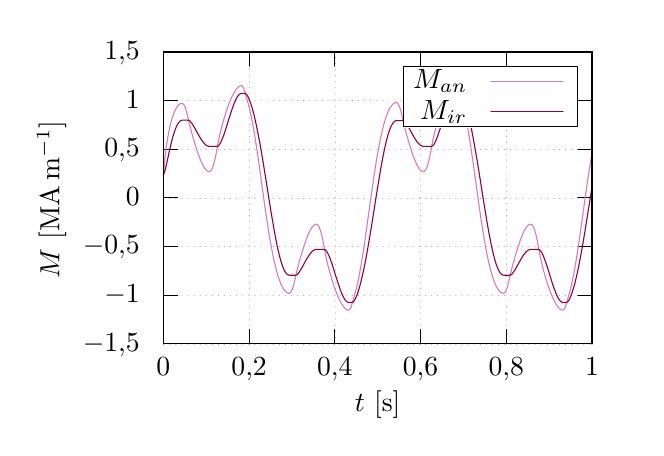
\begin{tikzpicture}[gnuplot]
%% generated with GNUPLOT 5.4p2 (Lua 5.4; terminal rev. Jun 2020, script rev. 114)
%% Fri 23 May 2025 09:04:49 AM -03
\path (0.000,0.000) rectangle (7.500,5.000);
\gpcolor{color=gp lt color axes}
\gpsetlinetype{gp lt axes}
\gpsetdashtype{gp dt axes}
\gpsetlinewidth{0.50}
\draw[gp path] (1.504,0.985)--(6.947,0.985);
\gpcolor{color=gp lt color border}
\gpsetlinetype{gp lt border}
\gpsetdashtype{gp dt solid}
\gpsetlinewidth{1.00}
\draw[gp path] (1.504,0.985)--(1.684,0.985);
\draw[gp path] (6.947,0.985)--(6.767,0.985);
\node[gp node right] at (1.320,0.985) {$-1,5$};
\gpcolor{color=gp lt color axes}
\gpsetlinetype{gp lt axes}
\gpsetdashtype{gp dt axes}
\gpsetlinewidth{0.50}
\draw[gp path] (1.504,1.603)--(6.947,1.603);
\gpcolor{color=gp lt color border}
\gpsetlinetype{gp lt border}
\gpsetdashtype{gp dt solid}
\gpsetlinewidth{1.00}
\draw[gp path] (1.504,1.603)--(1.684,1.603);
\draw[gp path] (6.947,1.603)--(6.767,1.603);
\node[gp node right] at (1.320,1.603) {$-1$};
\gpcolor{color=gp lt color axes}
\gpsetlinetype{gp lt axes}
\gpsetdashtype{gp dt axes}
\gpsetlinewidth{0.50}
\draw[gp path] (1.504,2.220)--(6.947,2.220);
\gpcolor{color=gp lt color border}
\gpsetlinetype{gp lt border}
\gpsetdashtype{gp dt solid}
\gpsetlinewidth{1.00}
\draw[gp path] (1.504,2.220)--(1.684,2.220);
\draw[gp path] (6.947,2.220)--(6.767,2.220);
\node[gp node right] at (1.320,2.220) {$-0,5$};
\gpcolor{color=gp lt color axes}
\gpsetlinetype{gp lt axes}
\gpsetdashtype{gp dt axes}
\gpsetlinewidth{0.50}
\draw[gp path] (1.504,2.838)--(6.947,2.838);
\gpcolor{color=gp lt color border}
\gpsetlinetype{gp lt border}
\gpsetdashtype{gp dt solid}
\gpsetlinewidth{1.00}
\draw[gp path] (1.504,2.838)--(1.684,2.838);
\draw[gp path] (6.947,2.838)--(6.767,2.838);
\node[gp node right] at (1.320,2.838) {$0$};
\gpcolor{color=gp lt color axes}
\gpsetlinetype{gp lt axes}
\gpsetdashtype{gp dt axes}
\gpsetlinewidth{0.50}
\draw[gp path] (1.504,3.456)--(6.947,3.456);
\gpcolor{color=gp lt color border}
\gpsetlinetype{gp lt border}
\gpsetdashtype{gp dt solid}
\gpsetlinewidth{1.00}
\draw[gp path] (1.504,3.456)--(1.684,3.456);
\draw[gp path] (6.947,3.456)--(6.767,3.456);
\node[gp node right] at (1.320,3.456) {$0,5$};
\gpcolor{color=gp lt color axes}
\gpsetlinetype{gp lt axes}
\gpsetdashtype{gp dt axes}
\gpsetlinewidth{0.50}
\draw[gp path] (1.504,4.073)--(4.559,4.073);
\draw[gp path] (6.763,4.073)--(6.947,4.073);
\gpcolor{color=gp lt color border}
\gpsetlinetype{gp lt border}
\gpsetdashtype{gp dt solid}
\gpsetlinewidth{1.00}
\draw[gp path] (1.504,4.073)--(1.684,4.073);
\draw[gp path] (6.947,4.073)--(6.767,4.073);
\node[gp node right] at (1.320,4.073) {$1$};
\gpcolor{color=gp lt color axes}
\gpsetlinetype{gp lt axes}
\gpsetdashtype{gp dt axes}
\gpsetlinewidth{0.50}
\draw[gp path] (1.504,4.691)--(6.947,4.691);
\gpcolor{color=gp lt color border}
\gpsetlinetype{gp lt border}
\gpsetdashtype{gp dt solid}
\gpsetlinewidth{1.00}
\draw[gp path] (1.504,4.691)--(1.684,4.691);
\draw[gp path] (6.947,4.691)--(6.767,4.691);
\node[gp node right] at (1.320,4.691) {$1,5$};
\gpcolor{color=gp lt color axes}
\gpsetlinetype{gp lt axes}
\gpsetdashtype{gp dt axes}
\gpsetlinewidth{0.50}
\draw[gp path] (1.504,0.985)--(1.504,4.691);
\gpcolor{color=gp lt color border}
\gpsetlinetype{gp lt border}
\gpsetdashtype{gp dt solid}
\gpsetlinewidth{1.00}
\draw[gp path] (1.504,0.985)--(1.504,1.165);
\draw[gp path] (1.504,4.691)--(1.504,4.511);
\node[gp node center] at (1.504,0.677) {$0$};
\gpcolor{color=gp lt color axes}
\gpsetlinetype{gp lt axes}
\gpsetdashtype{gp dt axes}
\gpsetlinewidth{0.50}
\draw[gp path] (2.593,0.985)--(2.593,4.691);
\gpcolor{color=gp lt color border}
\gpsetlinetype{gp lt border}
\gpsetdashtype{gp dt solid}
\gpsetlinewidth{1.00}
\draw[gp path] (2.593,0.985)--(2.593,1.165);
\draw[gp path] (2.593,4.691)--(2.593,4.511);
\node[gp node center] at (2.593,0.677) {$0,2$};
\gpcolor{color=gp lt color axes}
\gpsetlinetype{gp lt axes}
\gpsetdashtype{gp dt axes}
\gpsetlinewidth{0.50}
\draw[gp path] (3.681,0.985)--(3.681,4.691);
\gpcolor{color=gp lt color border}
\gpsetlinetype{gp lt border}
\gpsetdashtype{gp dt solid}
\gpsetlinewidth{1.00}
\draw[gp path] (3.681,0.985)--(3.681,1.165);
\draw[gp path] (3.681,4.691)--(3.681,4.511);
\node[gp node center] at (3.681,0.677) {$0,4$};
\gpcolor{color=gp lt color axes}
\gpsetlinetype{gp lt axes}
\gpsetdashtype{gp dt axes}
\gpsetlinewidth{0.50}
\draw[gp path] (4.770,0.985)--(4.770,3.741);
\draw[gp path] (4.770,4.511)--(4.770,4.691);
\gpcolor{color=gp lt color border}
\gpsetlinetype{gp lt border}
\gpsetdashtype{gp dt solid}
\gpsetlinewidth{1.00}
\draw[gp path] (4.770,0.985)--(4.770,1.165);
\draw[gp path] (4.770,4.691)--(4.770,4.511);
\node[gp node center] at (4.770,0.677) {$0,6$};
\gpcolor{color=gp lt color axes}
\gpsetlinetype{gp lt axes}
\gpsetdashtype{gp dt axes}
\gpsetlinewidth{0.50}
\draw[gp path] (5.858,0.985)--(5.858,3.741);
\draw[gp path] (5.858,4.511)--(5.858,4.691);
\gpcolor{color=gp lt color border}
\gpsetlinetype{gp lt border}
\gpsetdashtype{gp dt solid}
\gpsetlinewidth{1.00}
\draw[gp path] (5.858,0.985)--(5.858,1.165);
\draw[gp path] (5.858,4.691)--(5.858,4.511);
\node[gp node center] at (5.858,0.677) {$0,8$};
\gpcolor{color=gp lt color axes}
\gpsetlinetype{gp lt axes}
\gpsetdashtype{gp dt axes}
\gpsetlinewidth{0.50}
\draw[gp path] (6.947,0.985)--(6.947,4.691);
\gpcolor{color=gp lt color border}
\gpsetlinetype{gp lt border}
\gpsetdashtype{gp dt solid}
\gpsetlinewidth{1.00}
\draw[gp path] (6.947,0.985)--(6.947,1.165);
\draw[gp path] (6.947,4.691)--(6.947,4.511);
\node[gp node center] at (6.947,0.677) {$1$};
\draw[gp path] (1.504,4.691)--(1.504,0.985)--(6.947,0.985)--(6.947,4.691)--cycle;
\node[gp node center,rotate=-270] at (0.108,2.838) {$M$ [\si{\mega\ampere\per\meter}]};
\node[gp node center] at (4.225,0.215) {$t$ [\si{\second}]};
\draw[gp path] (4.559,3.741)--(4.559,4.511)--(6.763,4.511)--(6.763,3.741)--cycle;
\gpcolor{rgb color={0.831,0.488,0.735}}
\draw[gp path] (1.504,3.099)--(1.522,3.335)--(1.540,3.485)--(1.559,3.601)--(1.577,3.697)%
  --(1.595,3.777)--(1.613,3.844)--(1.631,3.899)--(1.650,3.944)--(1.668,3.979)--(1.686,4.006)%
  --(1.704,4.025)--(1.722,4.036)--(1.741,4.040)--(1.759,4.030)--(1.777,3.997)--(1.795,3.943)%
  --(1.813,3.871)--(1.832,3.787)--(1.850,3.717)--(1.868,3.651)--(1.886,3.588)--(1.904,3.527)%
  --(1.923,3.469)--(1.941,3.413)--(1.959,3.361)--(1.977,3.314)--(1.996,3.273)--(2.014,3.237)%
  --(2.032,3.209)--(2.050,3.188)--(2.068,3.175)--(2.087,3.171)--(2.105,3.180)--(2.123,3.210)%
  --(2.141,3.261)--(2.159,3.331)--(2.178,3.421)--(2.196,3.525)--(2.214,3.614)--(2.232,3.690)%
  --(2.250,3.761)--(2.269,3.826)--(2.287,3.887)--(2.305,3.944)--(2.323,3.996)--(2.341,4.045)%
  --(2.360,4.090)--(2.378,4.130)--(2.396,4.166)--(2.414,4.196)--(2.432,4.222)--(2.451,4.242)%
  --(2.469,4.256)--(2.487,4.263)--(2.505,4.261)--(2.523,4.233)--(2.542,4.175)--(2.560,4.110)%
  --(2.578,4.047)--(2.596,3.977)--(2.614,3.897)--(2.633,3.807)--(2.651,3.707)--(2.669,3.598)%
  --(2.687,3.481)--(2.705,3.358)--(2.724,3.230)--(2.742,3.099)--(2.760,2.967)--(2.778,2.836)%
  --(2.796,2.707)--(2.815,2.583)--(2.833,2.463)--(2.851,2.351)--(2.869,2.245)--(2.888,2.148)%
  --(2.906,2.059)--(2.924,1.979)--(2.942,1.907)--(2.960,1.844)--(2.979,1.790)--(2.997,1.744)%
  --(3.015,1.706)--(3.033,1.675)--(3.051,1.653)--(3.070,1.637)--(3.088,1.628)--(3.106,1.626)%
  --(3.124,1.642)--(3.142,1.681)--(3.161,1.739)--(3.179,1.816)--(3.197,1.901)--(3.215,1.972)%
  --(3.233,2.038)--(3.252,2.101)--(3.270,2.162)--(3.288,2.220)--(3.306,2.275)--(3.324,2.326)%
  --(3.343,2.372)--(3.361,2.412)--(3.379,2.446)--(3.397,2.472)--(3.415,2.491)--(3.434,2.502)%
  --(3.452,2.504)--(3.470,2.490)--(3.488,2.454)--(3.506,2.399)--(3.525,2.323)--(3.543,2.229)%
  --(3.561,2.126)--(3.579,2.042)--(3.597,1.967)--(3.616,1.899)--(3.634,1.835)--(3.652,1.775)%
  --(3.670,1.719)--(3.688,1.667)--(3.707,1.619)--(3.725,1.576)--(3.743,1.537)--(3.761,1.502)%
  --(3.780,1.473)--(3.798,1.448)--(3.816,1.430)--(3.834,1.418)--(3.852,1.412)--(3.871,1.420)%
  --(3.889,1.455)--(3.907,1.519)--(3.925,1.581)--(3.943,1.646)--(3.962,1.718)--(3.980,1.800)%
  --(3.998,1.893)--(4.016,1.995)--(4.034,2.106)--(4.053,2.225)--(4.071,2.350)--(4.089,2.479)%
  --(4.107,2.610)--(4.125,2.742)--(4.144,2.873)--(4.162,3.000)--(4.180,3.124)--(4.198,3.242)%
  --(4.216,3.353)--(4.235,3.456)--(4.253,3.551)--(4.271,3.638)--(4.289,3.716)--(4.307,3.785)%
  --(4.326,3.846)--(4.344,3.898)--(4.362,3.942)--(4.380,3.979)--(4.398,4.007)--(4.417,4.028)%
  --(4.435,4.042)--(4.453,4.049)--(4.471,4.048)--(4.489,4.026)--(4.508,3.983)--(4.526,3.919)%
  --(4.544,3.838)--(4.562,3.756)--(4.580,3.687)--(4.599,3.622)--(4.617,3.560)--(4.635,3.499)%
  --(4.653,3.442)--(4.671,3.388)--(4.690,3.338)--(4.708,3.294)--(4.726,3.255)--(4.744,3.223)%
  --(4.763,3.198)--(4.781,3.181)--(4.799,3.173)--(4.817,3.174)--(4.835,3.193)--(4.854,3.234)%
  --(4.872,3.294)--(4.890,3.374)--(4.908,3.473)--(4.926,3.572)--(4.945,3.653)--(4.963,3.726)%
  --(4.981,3.794)--(4.999,3.857)--(5.017,3.916)--(5.036,3.970)--(5.054,4.021)--(5.072,4.068)%
  --(5.090,4.110)--(5.108,4.148)--(5.127,4.182)--(5.145,4.210)--(5.163,4.233)--(5.181,4.250)%
  --(5.199,4.260)--(5.218,4.264)--(5.236,4.250)--(5.254,4.208)--(5.272,4.140)--(5.290,4.079)%
  --(5.309,4.013)--(5.327,3.938)--(5.345,3.853)--(5.363,3.758)--(5.381,3.654)--(5.400,3.541)%
  --(5.418,3.420)--(5.436,3.294)--(5.454,3.165)--(5.472,3.033)--(5.491,2.901)--(5.509,2.771)%
  --(5.527,2.644)--(5.545,2.522)--(5.563,2.406)--(5.582,2.297)--(5.600,2.195)--(5.618,2.102)%
  --(5.636,2.018)--(5.655,1.942)--(5.673,1.875)--(5.691,1.816)--(5.709,1.766)--(5.727,1.724)%
  --(5.746,1.690)--(5.764,1.663)--(5.782,1.644)--(5.800,1.632)--(5.818,1.626)--(5.837,1.631)%
  --(5.855,1.659)--(5.873,1.708)--(5.891,1.776)--(5.909,1.861)--(5.928,1.938)--(5.946,2.005)%
  --(5.964,2.070)--(5.982,2.132)--(6.000,2.191)--(6.019,2.248)--(6.037,2.301)--(6.055,2.349)%
  --(6.073,2.393)--(6.091,2.430)--(6.110,2.460)--(6.128,2.483)--(6.146,2.498)--(6.164,2.504)%
  --(6.182,2.499)--(6.201,2.475)--(6.219,2.429)--(6.237,2.363)--(6.255,2.279)--(6.273,2.176)%
  --(6.292,2.083)--(6.310,2.004)--(6.328,1.932)--(6.346,1.866)--(6.364,1.804)--(6.383,1.746)%
  --(6.401,1.692)--(6.419,1.643)--(6.437,1.597)--(6.455,1.556)--(6.474,1.519)--(6.492,1.487)%
  --(6.510,1.460)--(6.528,1.438)--(6.547,1.423)--(6.565,1.414)--(6.583,1.413)--(6.601,1.434)%
  --(6.619,1.484)--(6.638,1.551)--(6.656,1.613)--(6.674,1.681)--(6.692,1.758)--(6.710,1.845)%
  --(6.729,1.943)--(6.747,2.050)--(6.765,2.165)--(6.783,2.287)--(6.801,2.414)--(6.820,2.544)%
  --(6.838,2.676)--(6.856,2.808)--(6.874,2.937)--(6.892,3.063)--(6.911,3.183)--(6.929,3.298)%
  --(6.947,3.405);
\gpcolor{rgb color={0.569,0.000,0.247}}
\draw[gp path] (1.504,3.133)--(1.522,3.174)--(1.540,3.251)--(1.559,3.335)--(1.577,3.419)%
  --(1.595,3.498)--(1.613,3.572)--(1.631,3.637)--(1.650,3.694)--(1.668,3.741)--(1.686,3.777)%
  --(1.704,3.803)--(1.722,3.819)--(1.741,3.825)--(1.759,3.825)--(1.777,3.825)--(1.795,3.825)%
  --(1.813,3.825)--(1.832,3.822)--(1.850,3.806)--(1.868,3.782)--(1.886,3.753)--(1.904,3.722)%
  --(1.923,3.688)--(1.941,3.655)--(1.959,3.622)--(1.977,3.592)--(1.996,3.564)--(2.014,3.540)%
  --(2.032,3.520)--(2.050,3.505)--(2.068,3.496)--(2.087,3.492)--(2.105,3.492)--(2.123,3.492)%
  --(2.141,3.493)--(2.159,3.493)--(2.178,3.493)--(2.196,3.494)--(2.214,3.512)--(2.232,3.543)%
  --(2.250,3.583)--(2.269,3.631)--(2.287,3.684)--(2.305,3.740)--(2.323,3.799)--(2.341,3.857)%
  --(2.360,3.915)--(2.378,3.970)--(2.396,4.021)--(2.414,4.065)--(2.432,4.103)--(2.451,4.133)%
  --(2.469,4.154)--(2.487,4.164)--(2.505,4.166)--(2.523,4.166)--(2.542,4.166)--(2.560,4.154)%
  --(2.578,4.126)--(2.596,4.085)--(2.614,4.035)--(2.633,3.976)--(2.651,3.908)--(2.669,3.832)%
  --(2.687,3.749)--(2.705,3.659)--(2.724,3.563)--(2.742,3.461)--(2.760,3.355)--(2.778,3.245)%
  --(2.796,3.132)--(2.815,3.017)--(2.833,2.901)--(2.851,2.786)--(2.869,2.673)--(2.888,2.562)%
  --(2.906,2.456)--(2.924,2.356)--(2.942,2.263)--(2.960,2.178)--(2.979,2.101)--(2.997,2.035)%
  --(3.015,1.978)--(3.033,1.932)--(3.051,1.898)--(3.070,1.873)--(3.088,1.860)--(3.106,1.856)%
  --(3.124,1.856)--(3.142,1.856)--(3.161,1.856)--(3.179,1.856)--(3.197,1.860)--(3.215,1.877)%
  --(3.233,1.902)--(3.252,1.932)--(3.270,1.963)--(3.288,1.997)--(3.306,2.030)--(3.324,2.062)%
  --(3.343,2.092)--(3.361,2.119)--(3.379,2.142)--(3.397,2.161)--(3.415,2.174)--(3.434,2.182)%
  --(3.452,2.184)--(3.470,2.184)--(3.488,2.184)--(3.506,2.184)--(3.525,2.184)--(3.543,2.184)%
  --(3.561,2.179)--(3.579,2.158)--(3.597,2.124)--(3.616,2.082)--(3.634,2.033)--(3.652,1.979)%
  --(3.670,1.921)--(3.688,1.863)--(3.707,1.804)--(3.725,1.747)--(3.743,1.693)--(3.761,1.644)%
  --(3.780,1.600)--(3.798,1.565)--(3.816,1.537)--(3.834,1.519)--(3.852,1.511)--(3.871,1.510)%
  --(3.889,1.510)--(3.907,1.511)--(3.925,1.528)--(3.943,1.559)--(3.962,1.602)--(3.980,1.655)%
  --(3.998,1.717)--(4.016,1.786)--(4.034,1.864)--(4.053,1.949)--(4.071,2.041)--(4.089,2.138)%
  --(4.107,2.241)--(4.125,2.348)--(4.144,2.459)--(4.162,2.573)--(4.180,2.688)--(4.198,2.804)%
  --(4.216,2.919)--(4.235,3.031)--(4.253,3.141)--(4.271,3.245)--(4.289,3.344)--(4.307,3.435)%
  --(4.326,3.518)--(4.344,3.592)--(4.362,3.657)--(4.380,3.710)--(4.398,3.753)--(4.417,3.785)%
  --(4.435,3.807)--(4.453,3.818)--(4.471,3.820)--(4.489,3.820)--(4.508,3.820)--(4.526,3.820)%
  --(4.544,3.820)--(4.562,3.813)--(4.580,3.793)--(4.599,3.767)--(4.617,3.737)--(4.635,3.704)%
  --(4.653,3.671)--(4.671,3.638)--(4.690,3.606)--(4.708,3.577)--(4.726,3.551)--(4.744,3.529)%
  --(4.763,3.511)--(4.781,3.499)--(4.799,3.493)--(4.817,3.492)--(4.835,3.492)--(4.854,3.492)%
  --(4.872,3.492)--(4.890,3.492)--(4.908,3.492)--(4.926,3.501)--(4.945,3.526)--(4.963,3.562)%
  --(4.981,3.606)--(4.999,3.657)--(5.017,3.711)--(5.036,3.769)--(5.054,3.828)--(5.072,3.887)%
  --(5.090,3.943)--(5.108,3.996)--(5.127,4.044)--(5.145,4.085)--(5.163,4.119)--(5.181,4.144)%
  --(5.199,4.160)--(5.218,4.166)--(5.236,4.166)--(5.254,4.166)--(5.272,4.163)--(5.290,4.141)%
  --(5.309,4.107)--(5.327,4.061)--(5.345,4.007)--(5.363,3.943)--(5.381,3.871)--(5.400,3.791)%
  --(5.418,3.705)--(5.436,3.611)--(5.454,3.513)--(5.472,3.408)--(5.491,3.300)--(5.509,3.188)%
  --(5.527,3.074)--(5.545,2.959)--(5.563,2.843)--(5.582,2.729)--(5.600,2.617)--(5.618,2.509)%
  --(5.636,2.406)--(5.655,2.309)--(5.673,2.219)--(5.691,2.138)--(5.709,2.067)--(5.727,2.005)%
  --(5.746,1.954)--(5.764,1.914)--(5.782,1.884)--(5.800,1.865)--(5.818,1.857)--(5.837,1.856)%
  --(5.855,1.856)--(5.873,1.856)--(5.891,1.856)--(5.909,1.856)--(5.928,1.868)--(5.946,1.889)%
  --(5.964,1.917)--(5.982,1.947)--(6.000,1.980)--(6.019,2.013)--(6.037,2.046)--(6.055,2.077)%
  --(6.073,2.106)--(6.091,2.131)--(6.110,2.152)--(6.128,2.168)--(6.146,2.179)--(6.164,2.184)%
  --(6.182,2.184)--(6.201,2.184)--(6.219,2.184)--(6.237,2.184)--(6.255,2.184)--(6.273,2.184)%
  --(6.292,2.170)--(6.310,2.142)--(6.328,2.104)--(6.346,2.058)--(6.364,2.006)--(6.383,1.950)%
  --(6.401,1.892)--(6.419,1.833)--(6.437,1.775)--(6.455,1.719)--(6.474,1.668)--(6.492,1.621)%
  --(6.510,1.582)--(6.528,1.550)--(6.547,1.527)--(6.565,1.513)--(6.583,1.510)--(6.601,1.510)%
  --(6.619,1.510)--(6.638,1.517)--(6.656,1.542)--(6.674,1.580)--(6.692,1.627)--(6.710,1.685)%
  --(6.729,1.750)--(6.747,1.824)--(6.765,1.906)--(6.783,1.994)--(6.801,2.089)--(6.820,2.189)%
  --(6.838,2.294)--(6.856,2.404)--(6.874,2.516)--(6.892,2.630)--(6.911,2.746)--(6.929,2.861)%
  --(6.947,2.975);
\gpfill{color=gpbgfillcolor} (4.559,3.741)--(6.763,3.741)--(6.763,4.511)--(4.559,4.511)--cycle;
\gpcolor{color=gp lt color border}
\draw[gp path] (4.559,3.741)--(4.559,4.511)--(6.763,4.511)--(6.763,3.741)--cycle;
\node[gp node right] at (5.479,4.318) {\phantom{M}$M_{an}$};
\gpcolor{rgb color={0.831,0.488,0.735}}
\draw[gp path] (5.663,4.318)--(6.579,4.318);
\gpcolor{color=gp lt color border}
\node[gp node right] at (5.479,3.933) {\phantom{M}$M_{ir}$};
\gpcolor{rgb color={0.569,0.000,0.247}}
\draw[gp path] (5.663,3.933)--(6.579,3.933);
\gpcolor{color=gp lt color border}
\draw[gp path] (1.504,4.691)--(1.504,0.985)--(6.947,0.985)--(6.947,4.691)--cycle;
%% coordinates of the plot area
\gpdefrectangularnode{gp plot 1}{\pgfpoint{1.504cm}{0.985cm}}{\pgfpoint{6.947cm}{4.691cm}}
\end{tikzpicture}
%% gnuplot variables

    \vspace{-1cm}
    \caption{HHHHHHHHHHHHHHH}
  \end{minipage}%
\end{figure}

\newpage

\begin{figure}[!h]
  \begin{minipage}{.49\linewidth}
    \centering
    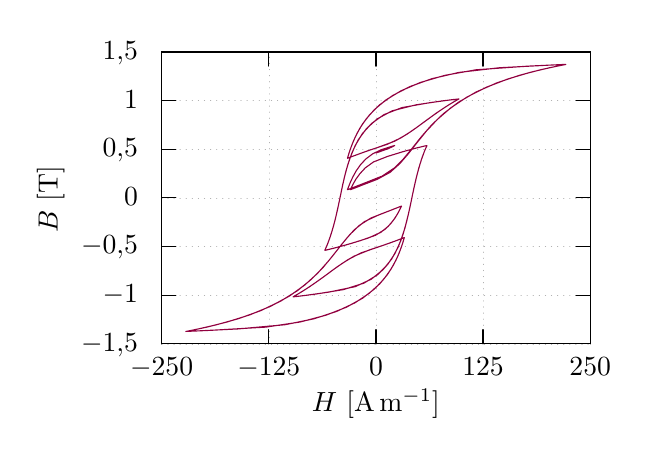
\begin{tikzpicture}[gnuplot]
%% generated with GNUPLOT 5.4p2 (Lua 5.4; terminal rev. Jun 2020, script rev. 114)
%% Fri 23 May 2025 09:04:29 AM -03
\path (0.000,0.000) rectangle (7.500,5.000);
\gpcolor{color=gp lt color axes}
\gpsetlinetype{gp lt axes}
\gpsetdashtype{gp dt axes}
\gpsetlinewidth{0.50}
\draw[gp path] (1.504,0.985)--(6.947,0.985);
\gpcolor{color=gp lt color border}
\gpsetlinetype{gp lt border}
\gpsetdashtype{gp dt solid}
\gpsetlinewidth{1.00}
\draw[gp path] (1.504,0.985)--(1.684,0.985);
\draw[gp path] (6.947,0.985)--(6.767,0.985);
\node[gp node right] at (1.320,0.985) {$-1,5$};
\gpcolor{color=gp lt color axes}
\gpsetlinetype{gp lt axes}
\gpsetdashtype{gp dt axes}
\gpsetlinewidth{0.50}
\draw[gp path] (1.504,1.603)--(6.947,1.603);
\gpcolor{color=gp lt color border}
\gpsetlinetype{gp lt border}
\gpsetdashtype{gp dt solid}
\gpsetlinewidth{1.00}
\draw[gp path] (1.504,1.603)--(1.684,1.603);
\draw[gp path] (6.947,1.603)--(6.767,1.603);
\node[gp node right] at (1.320,1.603) {$-1$};
\gpcolor{color=gp lt color axes}
\gpsetlinetype{gp lt axes}
\gpsetdashtype{gp dt axes}
\gpsetlinewidth{0.50}
\draw[gp path] (1.504,2.220)--(6.947,2.220);
\gpcolor{color=gp lt color border}
\gpsetlinetype{gp lt border}
\gpsetdashtype{gp dt solid}
\gpsetlinewidth{1.00}
\draw[gp path] (1.504,2.220)--(1.684,2.220);
\draw[gp path] (6.947,2.220)--(6.767,2.220);
\node[gp node right] at (1.320,2.220) {$-0,5$};
\gpcolor{color=gp lt color axes}
\gpsetlinetype{gp lt axes}
\gpsetdashtype{gp dt axes}
\gpsetlinewidth{0.50}
\draw[gp path] (1.504,2.838)--(6.947,2.838);
\gpcolor{color=gp lt color border}
\gpsetlinetype{gp lt border}
\gpsetdashtype{gp dt solid}
\gpsetlinewidth{1.00}
\draw[gp path] (1.504,2.838)--(1.684,2.838);
\draw[gp path] (6.947,2.838)--(6.767,2.838);
\node[gp node right] at (1.320,2.838) {$0$};
\gpcolor{color=gp lt color axes}
\gpsetlinetype{gp lt axes}
\gpsetdashtype{gp dt axes}
\gpsetlinewidth{0.50}
\draw[gp path] (1.504,3.456)--(6.947,3.456);
\gpcolor{color=gp lt color border}
\gpsetlinetype{gp lt border}
\gpsetdashtype{gp dt solid}
\gpsetlinewidth{1.00}
\draw[gp path] (1.504,3.456)--(1.684,3.456);
\draw[gp path] (6.947,3.456)--(6.767,3.456);
\node[gp node right] at (1.320,3.456) {$0,5$};
\gpcolor{color=gp lt color axes}
\gpsetlinetype{gp lt axes}
\gpsetdashtype{gp dt axes}
\gpsetlinewidth{0.50}
\draw[gp path] (1.504,4.073)--(6.947,4.073);
\gpcolor{color=gp lt color border}
\gpsetlinetype{gp lt border}
\gpsetdashtype{gp dt solid}
\gpsetlinewidth{1.00}
\draw[gp path] (1.504,4.073)--(1.684,4.073);
\draw[gp path] (6.947,4.073)--(6.767,4.073);
\node[gp node right] at (1.320,4.073) {$1$};
\gpcolor{color=gp lt color axes}
\gpsetlinetype{gp lt axes}
\gpsetdashtype{gp dt axes}
\gpsetlinewidth{0.50}
\draw[gp path] (1.504,4.691)--(6.947,4.691);
\gpcolor{color=gp lt color border}
\gpsetlinetype{gp lt border}
\gpsetdashtype{gp dt solid}
\gpsetlinewidth{1.00}
\draw[gp path] (1.504,4.691)--(1.684,4.691);
\draw[gp path] (6.947,4.691)--(6.767,4.691);
\node[gp node right] at (1.320,4.691) {$1,5$};
\gpcolor{color=gp lt color axes}
\gpsetlinetype{gp lt axes}
\gpsetdashtype{gp dt axes}
\gpsetlinewidth{0.50}
\draw[gp path] (1.504,0.985)--(1.504,4.691);
\gpcolor{color=gp lt color border}
\gpsetlinetype{gp lt border}
\gpsetdashtype{gp dt solid}
\gpsetlinewidth{1.00}
\draw[gp path] (1.504,0.985)--(1.504,1.165);
\draw[gp path] (1.504,4.691)--(1.504,4.511);
\node[gp node center] at (1.504,0.677) {$-250$};
\gpcolor{color=gp lt color axes}
\gpsetlinetype{gp lt axes}
\gpsetdashtype{gp dt axes}
\gpsetlinewidth{0.50}
\draw[gp path] (2.865,0.985)--(2.865,4.691);
\gpcolor{color=gp lt color border}
\gpsetlinetype{gp lt border}
\gpsetdashtype{gp dt solid}
\gpsetlinewidth{1.00}
\draw[gp path] (2.865,0.985)--(2.865,1.165);
\draw[gp path] (2.865,4.691)--(2.865,4.511);
\node[gp node center] at (2.865,0.677) {$-125$};
\gpcolor{color=gp lt color axes}
\gpsetlinetype{gp lt axes}
\gpsetdashtype{gp dt axes}
\gpsetlinewidth{0.50}
\draw[gp path] (4.226,0.985)--(4.226,4.691);
\gpcolor{color=gp lt color border}
\gpsetlinetype{gp lt border}
\gpsetdashtype{gp dt solid}
\gpsetlinewidth{1.00}
\draw[gp path] (4.226,0.985)--(4.226,1.165);
\draw[gp path] (4.226,4.691)--(4.226,4.511);
\node[gp node center] at (4.226,0.677) {$0$};
\gpcolor{color=gp lt color axes}
\gpsetlinetype{gp lt axes}
\gpsetdashtype{gp dt axes}
\gpsetlinewidth{0.50}
\draw[gp path] (5.586,0.985)--(5.586,4.691);
\gpcolor{color=gp lt color border}
\gpsetlinetype{gp lt border}
\gpsetdashtype{gp dt solid}
\gpsetlinewidth{1.00}
\draw[gp path] (5.586,0.985)--(5.586,1.165);
\draw[gp path] (5.586,4.691)--(5.586,4.511);
\node[gp node center] at (5.586,0.677) {$125$};
\gpcolor{color=gp lt color axes}
\gpsetlinetype{gp lt axes}
\gpsetdashtype{gp dt axes}
\gpsetlinewidth{0.50}
\draw[gp path] (6.947,0.985)--(6.947,4.691);
\gpcolor{color=gp lt color border}
\gpsetlinetype{gp lt border}
\gpsetdashtype{gp dt solid}
\gpsetlinewidth{1.00}
\draw[gp path] (6.947,0.985)--(6.947,1.165);
\draw[gp path] (6.947,4.691)--(6.947,4.511);
\node[gp node center] at (6.947,0.677) {$250$};
\draw[gp path] (1.504,4.691)--(1.504,0.985)--(6.947,0.985)--(6.947,4.691)--cycle;
\node[gp node center,rotate=-270] at (0.108,2.838) {$B$ [\si{\tesla}]};
\node[gp node center] at (4.225,0.215) {$H$ [\si{\ampere\per\meter}]};
\gpcolor{rgb color={0.569,0.000,0.247}}
\draw[gp path] (4.226,3.408)--(4.387,3.465)--(4.453,3.497)--(4.464,3.504)--(4.409,3.487)%
  --(4.293,3.450)--(4.183,3.397)--(4.096,3.331)--(4.028,3.257)--(3.975,3.181)--(3.935,3.109)%
  --(3.904,3.044)--(3.883,2.992)--(3.869,2.957)--(3.864,2.942)--(3.884,2.949)--(3.965,2.981)%
  --(4.108,3.037)--(4.307,3.116)--(4.457,3.216)--(4.576,3.335)--(4.686,3.468)--(4.800,3.612)%
  --(4.929,3.760)--(5.083,3.908)--(5.271,4.051)--(5.496,4.182)--(5.759,4.298)--(6.044,4.394)%
  --(6.319,4.466)--(6.535,4.513)--(6.637,4.533)--(6.442,4.525)--(5.792,4.491)--(5.281,4.432)%
  --(4.936,4.352)--(4.660,4.253)--(4.442,4.141)--(4.274,4.021)--(4.148,3.897)--(4.055,3.776)%
  --(3.988,3.662)--(3.940,3.560)--(3.907,3.474)--(3.884,3.408)--(3.871,3.364)--(3.865,3.343)%
  --(3.876,3.346)--(3.942,3.371)--(4.067,3.417)--(4.252,3.480)--(4.464,3.558)--(4.617,3.645)%
  --(4.748,3.736)--(4.871,3.827)--(4.988,3.912)--(5.097,3.985)--(5.189,4.043)--(5.253,4.080)%
  --(5.280,4.095)--(5.189,4.085)--(4.913,4.048)--(4.556,3.985)--(4.328,3.896)--(4.170,3.783)%
  --(4.051,3.651)--(3.962,3.502)--(3.895,3.342)--(3.844,3.175)--(3.804,3.007)--(3.770,2.843)%
  --(3.738,2.689)--(3.705,2.549)--(3.671,2.427)--(3.639,2.327)--(3.611,2.251)--(3.589,2.200)%
  --(3.578,2.175)--(3.588,2.174)--(3.679,2.196)--(3.836,2.238)--(4.027,2.295)--(4.220,2.363)%
  --(4.339,2.438)--(4.415,2.513)--(4.469,2.584)--(4.506,2.646)--(4.532,2.695)--(4.546,2.725)%
  --(4.551,2.734)--(4.516,2.721)--(4.419,2.683)--(4.261,2.622)--(4.080,2.537)--(3.950,2.432)%
  --(3.840,2.309)--(3.732,2.173)--(3.616,2.028)--(3.483,1.879)--(3.322,1.732)--(3.126,1.591)%
  --(2.891,1.463)--(2.622,1.352)--(2.335,1.262)--(2.070,1.195)--(1.878,1.155)--(1.811,1.142)%
  --(2.143,1.157)--(2.827,1.197)--(3.264,1.262)--(3.590,1.348)--(3.851,1.450)--(4.056,1.564)%
  --(4.212,1.686)--(4.329,1.810)--(4.415,1.930)--(4.477,2.041)--(4.521,2.139)--(4.551,2.220)%
  --(4.571,2.281)--(4.582,2.319)--(4.586,2.334)--(4.564,2.326)--(4.483,2.295)--(4.344,2.245)%
  --(4.142,2.177)--(3.945,2.097)--(3.800,2.008)--(3.671,1.917)--(3.550,1.827)--(3.434,1.745)%
  --(3.329,1.675)--(3.243,1.622)--(3.187,1.590)--(3.174,1.581)--(3.317,1.598)--(3.625,1.641)%
  --(3.963,1.711)--(4.167,1.806)--(4.314,1.924)--(4.425,2.061)--(4.508,2.213)--(4.570,2.375)%
  --(4.617,2.543)--(4.656,2.711)--(4.689,2.872)--(4.722,3.024)--(4.755,3.159)--(4.788,3.276)%
  --(4.819,3.370)--(4.846,3.440)--(4.865,3.484)--(4.874,3.503)--(4.848,3.498)--(4.737,3.471)%
  --(4.569,3.425)--(4.374,3.365)--(4.195,3.295)--(4.090,3.219)--(4.021,3.144)--(3.971,3.075)%
  --(3.937,3.016)--(3.915,2.972)--(3.902,2.947)--(3.903,2.943)--(3.954,2.962)--(4.065,3.006)%
  --(4.240,3.073)--(4.406,3.163)--(4.529,3.273)--(4.638,3.400)--(4.747,3.539)--(4.866,3.686)%
  --(5.005,3.834)--(5.174,3.980)--(5.380,4.118)--(5.624,4.242)--(5.900,4.348)--(6.186,4.433)%
  --(6.438,4.493)--(6.603,4.526)--(6.614,4.533)--(6.150,4.511)--(5.496,4.465)--(5.098,4.394)%
  --(4.790,4.304)--(4.544,4.198)--(4.352,4.082)--(4.206,3.959)--(4.098,3.836)--(4.019,3.718)%
  --(3.962,3.609)--(3.922,3.515)--(3.894,3.439)--(3.877,3.383)--(3.867,3.351)--(3.865,3.341)%
  --(3.902,3.356)--(3.997,3.391)--(4.152,3.447)--(4.368,3.518)--(4.545,3.601)--(4.684,3.690)%
  --(4.811,3.782)--(4.931,3.870)--(5.044,3.950)--(5.145,4.016)--(5.225,4.064)--(5.272,4.091)%
  --(5.261,4.093)--(5.069,4.070)--(4.734,4.020)--(4.429,3.943)--(4.243,3.842)--(4.107,3.720)%
  --(4.003,3.578)--(3.926,3.423)--(3.868,3.259)--(3.823,3.091)--(3.787,2.924)--(3.754,2.765)%
  --(3.721,2.617)--(3.688,2.485)--(3.655,2.374)--(3.624,2.286)--(3.599,2.223)--(3.582,2.185)%
  --(3.577,2.172)--(3.623,2.183)--(3.751,2.215)--(3.929,2.265)--(4.128,2.328)--(4.287,2.400)%
  --(4.381,2.476)--(4.444,2.550)--(4.489,2.617)--(4.521,2.673)--(4.540,2.712)--(4.550,2.733)%
  --(4.541,2.731)--(4.475,2.705)--(4.348,2.655)--(4.161,2.582)--(4.012,2.487)--(3.894,2.372)%
  --(3.786,2.242)--(3.676,2.101)--(3.553,1.953)--(3.407,1.805)--(3.229,1.660)--(3.014,1.526)%
  --(2.760,1.405)--(2.479,1.304)--(2.197,1.226)--(1.961,1.172)--(1.827,1.145)--(1.905,1.146)%
  --(2.475,1.174)--(3.068,1.227)--(3.437,1.302)--(3.728,1.397)--(3.960,1.506)--(4.139,1.625)%
  --(4.275,1.748)--(4.376,1.870)--(4.449,1.987)--(4.501,2.092)--(4.537,2.182)--(4.562,2.253)%
  --(4.577,2.303)--(4.585,2.330)--(4.582,2.333)--(4.531,2.313)--(4.421,2.272)--(4.251,2.213)%
  --(4.032,2.138)--(3.869,2.053)--(3.734,1.963)--(3.610,1.871)--(3.491,1.785)--(3.380,1.708)%
  --(3.283,1.646)--(3.211,1.603)--(3.174,1.582)--(3.220,1.586)--(3.457,1.616)--(3.812,1.673)%
  --(4.075,1.756)--(4.246,1.862)--(4.373,1.990)--(4.469,2.135)--(4.541,2.293)--(4.595,2.459)%
  --(4.637,2.627)--(4.673,2.793)--(4.705,2.950)--(4.738,3.094)--(4.771,3.220)--(4.804,3.326)%
  --(4.834,3.408);
\gpcolor{color=gp lt color border}
\draw[gp path] (1.504,4.691)--(1.504,0.985)--(6.947,0.985)--(6.947,4.691)--cycle;
%% coordinates of the plot area
\gpdefrectangularnode{gp plot 1}{\pgfpoint{1.504cm}{0.985cm}}{\pgfpoint{6.947cm}{4.691cm}}
\end{tikzpicture}
%% gnuplot variables

    \vspace{-1cm}
    \caption{uma caption}
  \end{minipage}%
  \begin{minipage}{.49\linewidth}
    \centering
    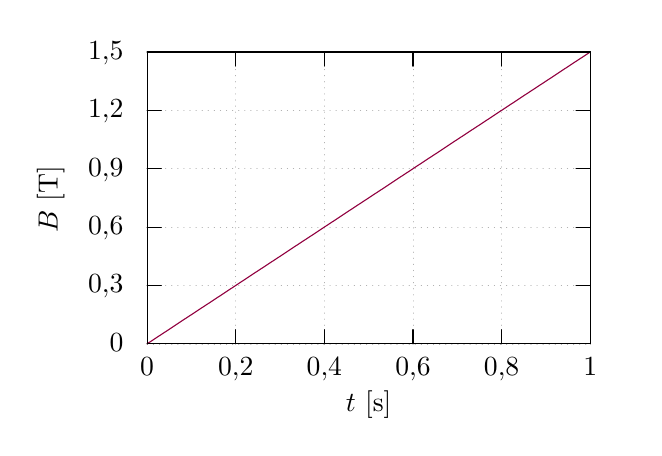
\begin{tikzpicture}[gnuplot]
%% generated with GNUPLOT 5.4p2 (Lua 5.4; terminal rev. Jun 2020, script rev. 114)
%% Fri 23 May 2025 09:06:32 AM -03
\path (0.000,0.000) rectangle (7.500,5.000);
\gpcolor{color=gp lt color axes}
\gpsetlinetype{gp lt axes}
\gpsetdashtype{gp dt axes}
\gpsetlinewidth{0.50}
\draw[gp path] (1.320,0.985)--(6.947,0.985);
\gpcolor{color=gp lt color border}
\gpsetlinetype{gp lt border}
\gpsetdashtype{gp dt solid}
\gpsetlinewidth{1.00}
\draw[gp path] (1.320,0.985)--(1.500,0.985);
\draw[gp path] (6.947,0.985)--(6.767,0.985);
\node[gp node right] at (1.136,0.985) {$0$};
\gpcolor{color=gp lt color axes}
\gpsetlinetype{gp lt axes}
\gpsetdashtype{gp dt axes}
\gpsetlinewidth{0.50}
\draw[gp path] (1.320,1.726)--(6.947,1.726);
\gpcolor{color=gp lt color border}
\gpsetlinetype{gp lt border}
\gpsetdashtype{gp dt solid}
\gpsetlinewidth{1.00}
\draw[gp path] (1.320,1.726)--(1.500,1.726);
\draw[gp path] (6.947,1.726)--(6.767,1.726);
\node[gp node right] at (1.136,1.726) {$0,3$};
\gpcolor{color=gp lt color axes}
\gpsetlinetype{gp lt axes}
\gpsetdashtype{gp dt axes}
\gpsetlinewidth{0.50}
\draw[gp path] (1.320,2.467)--(6.947,2.467);
\gpcolor{color=gp lt color border}
\gpsetlinetype{gp lt border}
\gpsetdashtype{gp dt solid}
\gpsetlinewidth{1.00}
\draw[gp path] (1.320,2.467)--(1.500,2.467);
\draw[gp path] (6.947,2.467)--(6.767,2.467);
\node[gp node right] at (1.136,2.467) {$0,6$};
\gpcolor{color=gp lt color axes}
\gpsetlinetype{gp lt axes}
\gpsetdashtype{gp dt axes}
\gpsetlinewidth{0.50}
\draw[gp path] (1.320,3.209)--(6.947,3.209);
\gpcolor{color=gp lt color border}
\gpsetlinetype{gp lt border}
\gpsetdashtype{gp dt solid}
\gpsetlinewidth{1.00}
\draw[gp path] (1.320,3.209)--(1.500,3.209);
\draw[gp path] (6.947,3.209)--(6.767,3.209);
\node[gp node right] at (1.136,3.209) {$0,9$};
\gpcolor{color=gp lt color axes}
\gpsetlinetype{gp lt axes}
\gpsetdashtype{gp dt axes}
\gpsetlinewidth{0.50}
\draw[gp path] (1.320,3.950)--(6.947,3.950);
\gpcolor{color=gp lt color border}
\gpsetlinetype{gp lt border}
\gpsetdashtype{gp dt solid}
\gpsetlinewidth{1.00}
\draw[gp path] (1.320,3.950)--(1.500,3.950);
\draw[gp path] (6.947,3.950)--(6.767,3.950);
\node[gp node right] at (1.136,3.950) {$1,2$};
\gpcolor{color=gp lt color axes}
\gpsetlinetype{gp lt axes}
\gpsetdashtype{gp dt axes}
\gpsetlinewidth{0.50}
\draw[gp path] (1.320,4.691)--(6.947,4.691);
\gpcolor{color=gp lt color border}
\gpsetlinetype{gp lt border}
\gpsetdashtype{gp dt solid}
\gpsetlinewidth{1.00}
\draw[gp path] (1.320,4.691)--(1.500,4.691);
\draw[gp path] (6.947,4.691)--(6.767,4.691);
\node[gp node right] at (1.136,4.691) {$1,5$};
\gpcolor{color=gp lt color axes}
\gpsetlinetype{gp lt axes}
\gpsetdashtype{gp dt axes}
\gpsetlinewidth{0.50}
\draw[gp path] (1.320,0.985)--(1.320,4.691);
\gpcolor{color=gp lt color border}
\gpsetlinetype{gp lt border}
\gpsetdashtype{gp dt solid}
\gpsetlinewidth{1.00}
\draw[gp path] (1.320,0.985)--(1.320,1.165);
\draw[gp path] (1.320,4.691)--(1.320,4.511);
\node[gp node center] at (1.320,0.677) {$0$};
\gpcolor{color=gp lt color axes}
\gpsetlinetype{gp lt axes}
\gpsetdashtype{gp dt axes}
\gpsetlinewidth{0.50}
\draw[gp path] (2.445,0.985)--(2.445,4.691);
\gpcolor{color=gp lt color border}
\gpsetlinetype{gp lt border}
\gpsetdashtype{gp dt solid}
\gpsetlinewidth{1.00}
\draw[gp path] (2.445,0.985)--(2.445,1.165);
\draw[gp path] (2.445,4.691)--(2.445,4.511);
\node[gp node center] at (2.445,0.677) {$0,2$};
\gpcolor{color=gp lt color axes}
\gpsetlinetype{gp lt axes}
\gpsetdashtype{gp dt axes}
\gpsetlinewidth{0.50}
\draw[gp path] (3.571,0.985)--(3.571,4.691);
\gpcolor{color=gp lt color border}
\gpsetlinetype{gp lt border}
\gpsetdashtype{gp dt solid}
\gpsetlinewidth{1.00}
\draw[gp path] (3.571,0.985)--(3.571,1.165);
\draw[gp path] (3.571,4.691)--(3.571,4.511);
\node[gp node center] at (3.571,0.677) {$0,4$};
\gpcolor{color=gp lt color axes}
\gpsetlinetype{gp lt axes}
\gpsetdashtype{gp dt axes}
\gpsetlinewidth{0.50}
\draw[gp path] (4.696,0.985)--(4.696,4.691);
\gpcolor{color=gp lt color border}
\gpsetlinetype{gp lt border}
\gpsetdashtype{gp dt solid}
\gpsetlinewidth{1.00}
\draw[gp path] (4.696,0.985)--(4.696,1.165);
\draw[gp path] (4.696,4.691)--(4.696,4.511);
\node[gp node center] at (4.696,0.677) {$0,6$};
\gpcolor{color=gp lt color axes}
\gpsetlinetype{gp lt axes}
\gpsetdashtype{gp dt axes}
\gpsetlinewidth{0.50}
\draw[gp path] (5.822,0.985)--(5.822,4.691);
\gpcolor{color=gp lt color border}
\gpsetlinetype{gp lt border}
\gpsetdashtype{gp dt solid}
\gpsetlinewidth{1.00}
\draw[gp path] (5.822,0.985)--(5.822,1.165);
\draw[gp path] (5.822,4.691)--(5.822,4.511);
\node[gp node center] at (5.822,0.677) {$0,8$};
\gpcolor{color=gp lt color axes}
\gpsetlinetype{gp lt axes}
\gpsetdashtype{gp dt axes}
\gpsetlinewidth{0.50}
\draw[gp path] (6.947,0.985)--(6.947,4.691);
\gpcolor{color=gp lt color border}
\gpsetlinetype{gp lt border}
\gpsetdashtype{gp dt solid}
\gpsetlinewidth{1.00}
\draw[gp path] (6.947,0.985)--(6.947,1.165);
\draw[gp path] (6.947,4.691)--(6.947,4.511);
\node[gp node center] at (6.947,0.677) {$1$};
\draw[gp path] (1.320,4.691)--(1.320,0.985)--(6.947,0.985)--(6.947,4.691)--cycle;
\node[gp node center,rotate=-270] at (0.108,2.838) {$B$ [\si{\tesla}]};
\node[gp node center] at (4.133,0.215) {$t$ [\si{\second}]};
\gpcolor{rgb color={0.569,0.000,0.247}}
\draw[gp path] (1.320,0.985)--(1.435,1.061)--(1.550,1.136)--(1.665,1.212)--(1.779,1.288)%
  --(1.894,1.363)--(2.009,1.439)--(2.124,1.514)--(2.239,1.590)--(2.354,1.666)--(2.468,1.741)%
  --(2.583,1.817)--(2.698,1.893)--(2.813,1.968)--(2.928,2.044)--(3.043,2.119)--(3.157,2.195)%
  --(3.272,2.271)--(3.387,2.346)--(3.502,2.422)--(3.617,2.498)--(3.732,2.573)--(3.846,2.649)%
  --(3.961,2.725)--(4.076,2.800)--(4.191,2.876)--(4.306,2.951)--(4.421,3.027)--(4.535,3.103)%
  --(4.650,3.178)--(4.765,3.254)--(4.880,3.330)--(4.995,3.405)--(5.110,3.481)--(5.224,3.557)%
  --(5.339,3.632)--(5.454,3.708)--(5.569,3.783)--(5.684,3.859)--(5.799,3.935)--(5.913,4.010)%
  --(6.028,4.086)--(6.143,4.162)--(6.258,4.237)--(6.373,4.313)--(6.488,4.388)--(6.602,4.464)%
  --(6.717,4.540)--(6.832,4.615)--(6.947,4.691);
\gpcolor{color=gp lt color border}
\draw[gp path] (1.320,4.691)--(1.320,0.985)--(6.947,0.985)--(6.947,4.691)--cycle;
%% coordinates of the plot area
\gpdefrectangularnode{gp plot 1}{\pgfpoint{1.320cm}{0.985cm}}{\pgfpoint{6.947cm}{4.691cm}}
\end{tikzpicture}
%% gnuplot variables

    \vspace{-1cm}
    \caption{HHHHHHHHHHHHHHH}
  \end{minipage}
  \begin{minipage}{.49\linewidth}
    \centering
    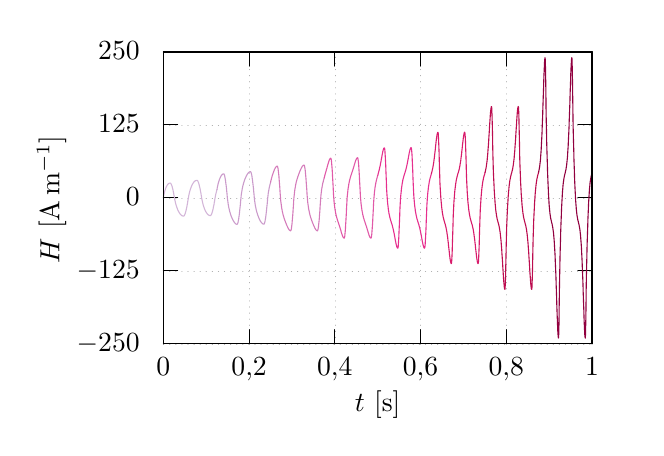
\begin{tikzpicture}[gnuplot]
%% generated with GNUPLOT 5.4p2 (Lua 5.4; terminal rev. Jun 2020, script rev. 114)
%% Fri 23 May 2025 09:05:47 AM -03
\path (0.000,0.000) rectangle (7.500,5.000);
\gpcolor{color=gp lt color axes}
\gpsetlinetype{gp lt axes}
\gpsetdashtype{gp dt axes}
\gpsetlinewidth{0.50}
\draw[gp path] (1.504,0.985)--(6.947,0.985);
\gpcolor{color=gp lt color border}
\gpsetlinetype{gp lt border}
\gpsetdashtype{gp dt solid}
\gpsetlinewidth{1.00}
\draw[gp path] (1.504,0.985)--(1.684,0.985);
\draw[gp path] (6.947,0.985)--(6.767,0.985);
\node[gp node right] at (1.320,0.985) {$-250$};
\gpcolor{color=gp lt color axes}
\gpsetlinetype{gp lt axes}
\gpsetdashtype{gp dt axes}
\gpsetlinewidth{0.50}
\draw[gp path] (1.504,1.912)--(6.947,1.912);
\gpcolor{color=gp lt color border}
\gpsetlinetype{gp lt border}
\gpsetdashtype{gp dt solid}
\gpsetlinewidth{1.00}
\draw[gp path] (1.504,1.912)--(1.684,1.912);
\draw[gp path] (6.947,1.912)--(6.767,1.912);
\node[gp node right] at (1.320,1.912) {$-125$};
\gpcolor{color=gp lt color axes}
\gpsetlinetype{gp lt axes}
\gpsetdashtype{gp dt axes}
\gpsetlinewidth{0.50}
\draw[gp path] (1.504,2.838)--(6.947,2.838);
\gpcolor{color=gp lt color border}
\gpsetlinetype{gp lt border}
\gpsetdashtype{gp dt solid}
\gpsetlinewidth{1.00}
\draw[gp path] (1.504,2.838)--(1.684,2.838);
\draw[gp path] (6.947,2.838)--(6.767,2.838);
\node[gp node right] at (1.320,2.838) {$0$};
\gpcolor{color=gp lt color axes}
\gpsetlinetype{gp lt axes}
\gpsetdashtype{gp dt axes}
\gpsetlinewidth{0.50}
\draw[gp path] (1.504,3.765)--(6.947,3.765);
\gpcolor{color=gp lt color border}
\gpsetlinetype{gp lt border}
\gpsetdashtype{gp dt solid}
\gpsetlinewidth{1.00}
\draw[gp path] (1.504,3.765)--(1.684,3.765);
\draw[gp path] (6.947,3.765)--(6.767,3.765);
\node[gp node right] at (1.320,3.765) {$125$};
\gpcolor{color=gp lt color axes}
\gpsetlinetype{gp lt axes}
\gpsetdashtype{gp dt axes}
\gpsetlinewidth{0.50}
\draw[gp path] (1.504,4.691)--(6.947,4.691);
\gpcolor{color=gp lt color border}
\gpsetlinetype{gp lt border}
\gpsetdashtype{gp dt solid}
\gpsetlinewidth{1.00}
\draw[gp path] (1.504,4.691)--(1.684,4.691);
\draw[gp path] (6.947,4.691)--(6.767,4.691);
\node[gp node right] at (1.320,4.691) {$250$};
\gpcolor{color=gp lt color axes}
\gpsetlinetype{gp lt axes}
\gpsetdashtype{gp dt axes}
\gpsetlinewidth{0.50}
\draw[gp path] (1.504,0.985)--(1.504,4.691);
\gpcolor{color=gp lt color border}
\gpsetlinetype{gp lt border}
\gpsetdashtype{gp dt solid}
\gpsetlinewidth{1.00}
\draw[gp path] (1.504,0.985)--(1.504,1.165);
\draw[gp path] (1.504,4.691)--(1.504,4.511);
\node[gp node center] at (1.504,0.677) {$0$};
\gpcolor{color=gp lt color axes}
\gpsetlinetype{gp lt axes}
\gpsetdashtype{gp dt axes}
\gpsetlinewidth{0.50}
\draw[gp path] (2.593,0.985)--(2.593,4.691);
\gpcolor{color=gp lt color border}
\gpsetlinetype{gp lt border}
\gpsetdashtype{gp dt solid}
\gpsetlinewidth{1.00}
\draw[gp path] (2.593,0.985)--(2.593,1.165);
\draw[gp path] (2.593,4.691)--(2.593,4.511);
\node[gp node center] at (2.593,0.677) {$0,2$};
\gpcolor{color=gp lt color axes}
\gpsetlinetype{gp lt axes}
\gpsetdashtype{gp dt axes}
\gpsetlinewidth{0.50}
\draw[gp path] (3.681,0.985)--(3.681,4.691);
\gpcolor{color=gp lt color border}
\gpsetlinetype{gp lt border}
\gpsetdashtype{gp dt solid}
\gpsetlinewidth{1.00}
\draw[gp path] (3.681,0.985)--(3.681,1.165);
\draw[gp path] (3.681,4.691)--(3.681,4.511);
\node[gp node center] at (3.681,0.677) {$0,4$};
\gpcolor{color=gp lt color axes}
\gpsetlinetype{gp lt axes}
\gpsetdashtype{gp dt axes}
\gpsetlinewidth{0.50}
\draw[gp path] (4.770,0.985)--(4.770,4.691);
\gpcolor{color=gp lt color border}
\gpsetlinetype{gp lt border}
\gpsetdashtype{gp dt solid}
\gpsetlinewidth{1.00}
\draw[gp path] (4.770,0.985)--(4.770,1.165);
\draw[gp path] (4.770,4.691)--(4.770,4.511);
\node[gp node center] at (4.770,0.677) {$0,6$};
\gpcolor{color=gp lt color axes}
\gpsetlinetype{gp lt axes}
\gpsetdashtype{gp dt axes}
\gpsetlinewidth{0.50}
\draw[gp path] (5.858,0.985)--(5.858,4.691);
\gpcolor{color=gp lt color border}
\gpsetlinetype{gp lt border}
\gpsetdashtype{gp dt solid}
\gpsetlinewidth{1.00}
\draw[gp path] (5.858,0.985)--(5.858,1.165);
\draw[gp path] (5.858,4.691)--(5.858,4.511);
\node[gp node center] at (5.858,0.677) {$0,8$};
\gpcolor{color=gp lt color axes}
\gpsetlinetype{gp lt axes}
\gpsetdashtype{gp dt axes}
\gpsetlinewidth{0.50}
\draw[gp path] (6.947,0.985)--(6.947,4.691);
\gpcolor{color=gp lt color border}
\gpsetlinetype{gp lt border}
\gpsetdashtype{gp dt solid}
\gpsetlinewidth{1.00}
\draw[gp path] (6.947,0.985)--(6.947,1.165);
\draw[gp path] (6.947,4.691)--(6.947,4.511);
\node[gp node center] at (6.947,0.677) {$1$};
\draw[gp path] (1.504,4.691)--(1.504,0.985)--(6.947,0.985)--(6.947,4.691)--cycle;
\node[gp node center,rotate=-270] at (0.108,2.838) {$H$ [\si{\ampere\per\meter}]};
\node[gp node center] at (4.225,0.215) {$t$ [\si{\second}]};
\gpcolor{rgb color={0.827,0.711,0.847}}
\draw[gp path] (1.504,2.838)--(1.507,2.856)--(1.509,2.871)--(1.512,2.885)--(1.515,2.898)%
  --(1.518,2.909)--(1.520,2.920)--(1.523,2.929)--(1.526,2.938)--(1.529,2.947)--(1.531,2.955)%
  --(1.534,2.962)--(1.537,2.969)--(1.539,2.975)--(1.542,2.981)--(1.545,2.986)--(1.548,2.991)%
  --(1.550,2.996)--(1.553,3.000)--(1.556,3.004)--(1.558,3.008)--(1.561,3.011)--(1.564,3.014)%
  --(1.567,3.016)--(1.569,3.019)--(1.572,3.021)--(1.575,3.022)--(1.578,3.024)--(1.580,3.025)%
  --(1.583,3.026)--(1.586,3.026)--(1.588,3.027)--(1.591,3.026)--(1.594,3.025)--(1.597,3.023)%
  --(1.599,3.019)--(1.602,3.015)--(1.605,3.009)--(1.607,3.003)--(1.610,2.996)--(1.613,2.988)%
  --(1.616,2.979)--(1.618,2.969)--(1.621,2.958)--(1.624,2.947)--(1.627,2.935)--(1.629,2.922)%
  --(1.632,2.908)--(1.635,2.894)--(1.637,2.879)--(1.640,2.864)--(1.643,2.848)--(1.646,2.833)%
  --(1.648,2.818)--(1.651,2.805)--(1.654,2.793)--(1.656,2.781)--(1.659,2.770)--(1.662,2.760)%
  --(1.665,2.750)--(1.667,2.741)--(1.670,2.732)--(1.673,2.724)--(1.676,2.716)--(1.678,2.709)%
  --(1.681,2.701)--(1.684,2.695)--(1.686,2.688)--(1.689,2.682)--(1.692,2.676)--(1.695,2.670)%
  --(1.697,2.665)--(1.700,2.660)--(1.703,2.655)--(1.705,2.650)--(1.708,2.646)--(1.711,2.642)%
  --(1.714,2.638)--(1.716,2.635)--(1.719,2.631)--(1.722,2.628)--(1.725,2.625)--(1.727,2.622)%
  --(1.730,2.620)--(1.733,2.618)--(1.735,2.616)--(1.738,2.614)--(1.741,2.612)--(1.744,2.611)%
  --(1.746,2.610)--(1.749,2.609)--(1.752,2.608)--(1.755,2.607)--(1.757,2.607)--(1.760,2.607)%
  --(1.763,2.608)--(1.765,2.610)--(1.768,2.613)--(1.771,2.617)--(1.774,2.622)--(1.776,2.628)%
  --(1.779,2.635)--(1.782,2.643)--(1.784,2.651)--(1.787,2.661)--(1.790,2.672)--(1.793,2.683)%
  --(1.795,2.695)--(1.798,2.708)--(1.801,2.721)--(1.804,2.735)--(1.806,2.750)--(1.809,2.765)%
  --(1.812,2.780)--(1.814,2.796)--(1.817,2.813)--(1.820,2.830)--(1.823,2.847)--(1.825,2.861)%
  --(1.828,2.875)--(1.831,2.888)--(1.833,2.899)--(1.836,2.910)--(1.839,2.921)--(1.842,2.930)%
  --(1.844,2.940)--(1.847,2.948)--(1.850,2.956)--(1.853,2.964)--(1.855,2.972)--(1.858,2.978)%
  --(1.861,2.985)--(1.863,2.991)--(1.866,2.997)--(1.869,3.003)--(1.872,3.008)--(1.874,3.013)%
  --(1.877,3.018)--(1.880,3.023)--(1.882,3.027)--(1.885,3.031)--(1.888,3.035)--(1.891,3.038)%
  --(1.893,3.041)--(1.896,3.044)--(1.899,3.047)--(1.902,3.049)--(1.904,3.052)--(1.907,3.054)%
  --(1.910,3.055)--(1.912,3.057)--(1.915,3.058)--(1.918,3.059)--(1.921,3.060)--(1.923,3.061)%
  --(1.926,3.061)--(1.929,3.061)--(1.931,3.061)--(1.934,3.060)--(1.937,3.057)--(1.940,3.054)%
  --(1.942,3.049)--(1.945,3.044)--(1.948,3.037)--(1.951,3.030)--(1.953,3.022)--(1.956,3.012)%
  --(1.959,3.002)--(1.961,2.991)--(1.964,2.980)--(1.967,2.967)--(1.970,2.954)--(1.972,2.941)%
  --(1.975,2.926)--(1.978,2.911)--(1.981,2.896)--(1.983,2.880)--(1.986,2.864)--(1.989,2.847)%
  --(1.991,2.831)--(1.994,2.816)--(1.997,2.802)--(2.000,2.789)--(2.002,2.778)--(2.005,2.767)%
  --(2.008,2.756)--(2.010,2.747)--(2.013,2.737)--(2.016,2.729)--(2.019,2.721)--(2.021,2.713)%
  --(2.024,2.705)--(2.027,2.698)--(2.030,2.692)--(2.032,2.685)--(2.035,2.679)--(2.038,2.674)%
  --(2.040,2.668)--(2.043,2.663)--(2.046,2.658)--(2.049,2.654)--(2.051,2.649)--(2.054,2.645)%
  --(2.057,2.642)--(2.059,2.638)--(2.062,2.635)--(2.065,2.632)--(2.068,2.629)--(2.070,2.626)%
  --(2.073,2.624)--(2.076,2.622)--(2.079,2.620)--(2.081,2.618)--(2.084,2.617)--(2.087,2.616)%
  --(2.089,2.615)--(2.092,2.614)--(2.095,2.614)--(2.098,2.613)--(2.100,2.613)--(2.103,2.614)%
  --(2.106,2.616)--(2.108,2.619)--(2.111,2.623)--(2.114,2.628)--(2.117,2.634)--(2.119,2.641)%
  --(2.122,2.649)--(2.125,2.658)--(2.128,2.668)--(2.130,2.678)--(2.133,2.689)--(2.136,2.701)%
  --(2.138,2.714)--(2.141,2.728)--(2.144,2.742)--(2.147,2.756)--(2.149,2.771)--(2.152,2.787)%
  --(2.155,2.803)--(2.157,2.820)--(2.160,2.837)--(2.163,2.852)--(2.166,2.867)--(2.168,2.880)%
  --(2.171,2.892)--(2.174,2.904)--(2.177,2.914)--(2.179,2.924)--(2.182,2.934)--(2.185,2.944);
\gpcolor{rgb color={0.797,0.609,0.795}}
\draw[gp path] (2.185,2.944)--(2.187,2.960)--(2.190,2.975)--(2.193,2.989)--(2.196,3.001)%
  --(2.198,3.013)--(2.201,3.024)--(2.204,3.034)--(2.206,3.043)--(2.209,3.052)--(2.212,3.060)%
  --(2.215,3.068)--(2.217,3.075)--(2.220,3.082)--(2.223,3.089)--(2.226,3.095)--(2.228,3.101)%
  --(2.231,3.106)--(2.234,3.111)--(2.236,3.116)--(2.239,3.120)--(2.242,3.124)--(2.245,3.128)%
  --(2.247,3.131)--(2.250,3.134)--(2.253,3.137)--(2.256,3.139)--(2.258,3.141)--(2.261,3.142)%
  --(2.264,3.143)--(2.266,3.144)--(2.269,3.144)--(2.272,3.143)--(2.275,3.140)--(2.277,3.134)%
  --(2.280,3.126)--(2.283,3.115)--(2.285,3.102)--(2.288,3.087)--(2.291,3.071)--(2.294,3.052)%
  --(2.296,3.032)--(2.299,3.010)--(2.302,2.986)--(2.305,2.961)--(2.307,2.935)--(2.310,2.908)%
  --(2.313,2.880)--(2.315,2.851)--(2.318,2.825)--(2.321,2.803)--(2.324,2.783)--(2.326,2.765)%
  --(2.329,2.748)--(2.332,2.733)--(2.334,2.719)--(2.337,2.706)--(2.340,2.694)--(2.343,2.682)%
  --(2.345,2.671)--(2.348,2.661)--(2.351,2.651)--(2.354,2.642)--(2.356,2.633)--(2.359,2.625)%
  --(2.362,2.617)--(2.364,2.609)--(2.367,2.602)--(2.370,2.595)--(2.373,2.589)--(2.375,2.582)%
  --(2.378,2.576)--(2.381,2.570)--(2.383,2.564)--(2.386,2.559)--(2.389,2.554)--(2.392,2.549)%
  --(2.394,2.544)--(2.397,2.540)--(2.400,2.535)--(2.403,2.531)--(2.405,2.527)--(2.408,2.524)%
  --(2.411,2.520)--(2.413,2.517)--(2.416,2.515)--(2.419,2.512)--(2.422,2.510)--(2.424,2.508)%
  --(2.427,2.506)--(2.430,2.505)--(2.432,2.504)--(2.435,2.503)--(2.438,2.503)--(2.441,2.503)%
  --(2.443,2.506)--(2.446,2.511)--(2.449,2.518)--(2.452,2.527)--(2.454,2.539)--(2.457,2.554)%
  --(2.460,2.570)--(2.462,2.588)--(2.465,2.608)--(2.468,2.629)--(2.471,2.653)--(2.473,2.677)%
  --(2.476,2.703)--(2.479,2.730)--(2.482,2.758)--(2.484,2.787)--(2.487,2.817)--(2.490,2.845)%
  --(2.492,2.869)--(2.495,2.890)--(2.498,2.908)--(2.501,2.925)--(2.503,2.941)--(2.506,2.956)%
  --(2.509,2.969)--(2.511,2.981)--(2.514,2.993)--(2.517,3.004)--(2.520,3.015)--(2.522,3.024)%
  --(2.525,3.034)--(2.528,3.043)--(2.531,3.051)--(2.533,3.059)--(2.536,3.067)--(2.539,3.074)%
  --(2.541,3.081)--(2.544,3.088)--(2.547,3.094)--(2.550,3.100)--(2.552,3.106)--(2.555,3.112)%
  --(2.558,3.117)--(2.560,3.122)--(2.563,3.127)--(2.566,3.132)--(2.569,3.137)--(2.571,3.141)%
  --(2.574,3.145)--(2.577,3.149)--(2.580,3.152)--(2.582,3.155)--(2.585,3.158)--(2.588,3.161)%
  --(2.590,3.163)--(2.593,3.165)--(2.596,3.167)--(2.599,3.169)--(2.601,3.170)--(2.604,3.171)%
  --(2.607,3.171)--(2.609,3.171)--(2.612,3.170)--(2.615,3.166)--(2.618,3.160)--(2.620,3.152)%
  --(2.623,3.141)--(2.626,3.128)--(2.629,3.112)--(2.631,3.095)--(2.634,3.076)--(2.637,3.055)%
  --(2.639,3.033)--(2.642,3.009)--(2.645,2.984)--(2.648,2.958)--(2.650,2.930)--(2.653,2.902)%
  --(2.656,2.872)--(2.658,2.843)--(2.661,2.817)--(2.664,2.795)--(2.667,2.775)--(2.669,2.758)%
  --(2.672,2.741)--(2.675,2.727)--(2.678,2.713)--(2.680,2.700)--(2.683,2.688)--(2.686,2.676)%
  --(2.688,2.666)--(2.691,2.656)--(2.694,2.646)--(2.697,2.637)--(2.699,2.629)--(2.702,2.620)%
  --(2.705,2.613)--(2.708,2.605)--(2.710,2.598)--(2.713,2.591)--(2.716,2.585)--(2.718,2.578)%
  --(2.721,2.572)--(2.724,2.567)--(2.727,2.561)--(2.729,2.556)--(2.732,2.551)--(2.735,2.546)%
  --(2.737,2.541)--(2.740,2.537)--(2.743,2.533)--(2.746,2.529)--(2.748,2.525)--(2.751,2.522)%
  --(2.754,2.519)--(2.757,2.516)--(2.759,2.514)--(2.762,2.511)--(2.765,2.510)--(2.767,2.508)%
  --(2.770,2.507)--(2.773,2.506)--(2.776,2.505)--(2.778,2.505)--(2.781,2.505)--(2.784,2.507)%
  --(2.786,2.512)--(2.789,2.520)--(2.792,2.530)--(2.795,2.542)--(2.797,2.556)--(2.800,2.572)%
  --(2.803,2.591)--(2.806,2.611)--(2.808,2.632)--(2.811,2.655)--(2.814,2.680)--(2.816,2.706)%
  --(2.819,2.733)--(2.822,2.761)--(2.825,2.790)--(2.827,2.820)--(2.830,2.847)--(2.833,2.871)%
  --(2.835,2.892)--(2.838,2.910)--(2.841,2.927)--(2.844,2.943)--(2.846,2.957)--(2.849,2.970)%
  --(2.852,2.983)--(2.855,2.994)--(2.857,3.005)--(2.860,3.016)--(2.863,3.025)--(2.865,3.036);
\gpcolor{rgb color={0.831,0.488,0.735}}
\draw[gp path] (2.865,3.036)--(2.868,3.049)--(2.871,3.061)--(2.874,3.072)--(2.876,3.083)%
  --(2.879,3.093)--(2.882,3.103)--(2.884,3.112)--(2.887,3.121)--(2.890,3.130)--(2.893,3.138)%
  --(2.895,3.146)--(2.898,3.154)--(2.901,3.162)--(2.904,3.169)--(2.906,3.177)--(2.909,3.183)%
  --(2.912,3.190)--(2.914,3.197)--(2.917,3.203)--(2.920,3.208)--(2.923,3.214)--(2.925,3.219)%
  --(2.928,3.223)--(2.931,3.227)--(2.934,3.231)--(2.936,3.234)--(2.939,3.237)--(2.942,3.239)%
  --(2.944,3.240)--(2.947,3.241)--(2.950,3.241)--(2.953,3.239)--(2.955,3.232)--(2.958,3.221)%
  --(2.961,3.205)--(2.963,3.185)--(2.966,3.162)--(2.969,3.135)--(2.972,3.105)--(2.974,3.073)%
  --(2.977,3.038)--(2.980,3.001)--(2.983,2.963)--(2.985,2.923)--(2.988,2.882)--(2.991,2.845)%
  --(2.993,2.814)--(2.996,2.788)--(2.999,2.765)--(3.002,2.744)--(3.004,2.725)--(3.007,2.708)%
  --(3.010,2.692)--(3.012,2.678)--(3.015,2.664)--(3.018,2.651)--(3.021,2.640)--(3.023,2.628)%
  --(3.026,2.618)--(3.029,2.608)--(3.032,2.599)--(3.034,2.590)--(3.037,2.581)--(3.040,2.573)%
  --(3.042,2.565)--(3.045,2.557)--(3.048,2.550)--(3.051,2.542)--(3.053,2.535)--(3.056,2.528)%
  --(3.059,2.521)--(3.061,2.514)--(3.064,2.508)--(3.067,2.501)--(3.070,2.494)--(3.072,2.488)%
  --(3.075,2.482)--(3.078,2.476)--(3.081,2.470)--(3.083,2.464)--(3.086,2.458)--(3.089,2.453)%
  --(3.091,2.448)--(3.094,2.443)--(3.097,2.439)--(3.100,2.435)--(3.102,2.431)--(3.105,2.428)%
  --(3.108,2.426)--(3.110,2.423)--(3.113,2.422)--(3.116,2.421)--(3.119,2.420)--(3.121,2.421)%
  --(3.124,2.426)--(3.127,2.435)--(3.130,2.449)--(3.132,2.467)--(3.135,2.489)--(3.138,2.515)%
  --(3.140,2.543)--(3.143,2.575)--(3.146,2.609)--(3.149,2.645)--(3.151,2.683)--(3.154,2.723)%
  --(3.157,2.763)--(3.159,2.805)--(3.162,2.841)--(3.165,2.870)--(3.168,2.896)--(3.170,2.918)%
  --(3.173,2.939)--(3.176,2.957)--(3.179,2.974)--(3.181,2.989)--(3.184,3.004)--(3.187,3.017)%
  --(3.189,3.029)--(3.192,3.041)--(3.195,3.052)--(3.198,3.062)--(3.200,3.072)--(3.203,3.081)%
  --(3.206,3.090)--(3.209,3.098)--(3.211,3.106)--(3.214,3.114)--(3.217,3.122)--(3.219,3.129)%
  --(3.222,3.137)--(3.225,3.144)--(3.228,3.151)--(3.230,3.158)--(3.233,3.165)--(3.236,3.171)%
  --(3.238,3.178)--(3.241,3.185)--(3.244,3.191)--(3.247,3.197)--(3.249,3.203)--(3.252,3.209)%
  --(3.255,3.215)--(3.258,3.220)--(3.260,3.225)--(3.263,3.230)--(3.266,3.235)--(3.268,3.239)%
  --(3.271,3.243)--(3.274,3.246)--(3.277,3.249)--(3.279,3.251)--(3.282,3.253)--(3.285,3.254)%
  --(3.287,3.255)--(3.290,3.255)--(3.293,3.253)--(3.296,3.245)--(3.298,3.233)--(3.301,3.217)%
  --(3.304,3.197)--(3.307,3.173)--(3.309,3.146)--(3.312,3.116)--(3.315,3.083)--(3.317,3.048)%
  --(3.320,3.011)--(3.323,2.972)--(3.326,2.932)--(3.328,2.890)--(3.331,2.851)--(3.334,2.819)%
  --(3.336,2.791)--(3.339,2.768)--(3.342,2.746)--(3.345,2.727)--(3.347,2.710)--(3.350,2.694)%
  --(3.353,2.679)--(3.356,2.665)--(3.358,2.653)--(3.361,2.641)--(3.364,2.629)--(3.366,2.619)%
  --(3.369,2.609)--(3.372,2.599)--(3.375,2.590)--(3.377,2.582)--(3.380,2.573)--(3.383,2.565)%
  --(3.385,2.558)--(3.388,2.550)--(3.391,2.543)--(3.394,2.535)--(3.396,2.528)--(3.399,2.521)%
  --(3.402,2.514)--(3.405,2.508)--(3.407,2.501)--(3.410,2.494)--(3.413,2.488)--(3.415,2.482)%
  --(3.418,2.476)--(3.421,2.470)--(3.424,2.464)--(3.426,2.458)--(3.429,2.453)--(3.432,2.448)%
  --(3.435,2.443)--(3.437,2.439)--(3.440,2.435)--(3.443,2.431)--(3.445,2.428)--(3.448,2.426)%
  --(3.451,2.424)--(3.454,2.422)--(3.456,2.421)--(3.459,2.420)--(3.462,2.421)--(3.464,2.427)%
  --(3.467,2.436)--(3.470,2.450)--(3.473,2.469)--(3.475,2.491)--(3.478,2.517)--(3.481,2.545)%
  --(3.484,2.577)--(3.486,2.611)--(3.489,2.647)--(3.492,2.685)--(3.494,2.725)--(3.497,2.766)%
  --(3.500,2.808)--(3.503,2.843)--(3.505,2.872)--(3.508,2.897)--(3.511,2.920)--(3.513,2.940)%
  --(3.516,2.958)--(3.519,2.975)--(3.522,2.990)--(3.524,3.004)--(3.527,3.018)--(3.530,3.030)%
  --(3.533,3.041)--(3.535,3.052)--(3.538,3.062)--(3.541,3.072)--(3.543,3.081)--(3.546,3.091);
\gpcolor{rgb color={0.881,0.349,0.660}}
\draw[gp path] (3.546,3.091)--(3.549,3.103)--(3.552,3.113)--(3.554,3.124)--(3.557,3.134)%
  --(3.560,3.143)--(3.562,3.153)--(3.565,3.163)--(3.568,3.172)--(3.571,3.182)--(3.573,3.192)%
  --(3.576,3.201)--(3.579,3.211)--(3.582,3.221)--(3.584,3.231)--(3.587,3.241)--(3.590,3.251)%
  --(3.592,3.260)--(3.595,3.270)--(3.598,3.279)--(3.601,3.288)--(3.603,3.296)--(3.606,3.304)%
  --(3.609,3.312)--(3.611,3.319)--(3.614,3.325)--(3.617,3.330)--(3.620,3.334)--(3.622,3.338)%
  --(3.625,3.340)--(3.628,3.342)--(3.631,3.342)--(3.633,3.337)--(3.636,3.324)--(3.639,3.303)%
  --(3.641,3.276)--(3.644,3.243)--(3.647,3.204)--(3.650,3.161)--(3.652,3.114)--(3.655,3.065)%
  --(3.658,3.012)--(3.661,2.958)--(3.663,2.904)--(3.666,2.861)--(3.669,2.825)--(3.671,2.794)%
  --(3.674,2.768)--(3.677,2.744)--(3.680,2.722)--(3.682,2.703)--(3.685,2.685)--(3.688,2.669)%
  --(3.690,2.654)--(3.693,2.640)--(3.696,2.627)--(3.699,2.615)--(3.701,2.604)--(3.704,2.594)%
  --(3.707,2.584)--(3.710,2.574)--(3.712,2.565)--(3.715,2.557)--(3.718,2.548)--(3.720,2.540)%
  --(3.723,2.532)--(3.726,2.524)--(3.729,2.516)--(3.731,2.508)--(3.734,2.499)--(3.737,2.491)%
  --(3.739,2.483)--(3.742,2.474)--(3.745,2.465)--(3.748,2.456)--(3.750,2.447)--(3.753,2.438)%
  --(3.756,2.429)--(3.759,2.420)--(3.761,2.410)--(3.764,2.401)--(3.767,2.392)--(3.769,2.384)%
  --(3.772,2.375)--(3.775,2.367)--(3.778,2.360)--(3.780,2.353)--(3.783,2.347)--(3.786,2.341)%
  --(3.788,2.337)--(3.791,2.333)--(3.794,2.330)--(3.797,2.328)--(3.799,2.327)--(3.802,2.329)%
  --(3.805,2.339)--(3.808,2.356)--(3.810,2.380)--(3.813,2.411)--(3.816,2.447)--(3.818,2.488)%
  --(3.821,2.534)--(3.824,2.583)--(3.827,2.634)--(3.829,2.687)--(3.832,2.742)--(3.835,2.793)%
  --(3.837,2.833)--(3.840,2.866)--(3.843,2.895)--(3.846,2.920)--(3.848,2.943)--(3.851,2.963)%
  --(3.854,2.982)--(3.857,2.999)--(3.859,3.015)--(3.862,3.029)--(3.865,3.043)--(3.867,3.055)%
  --(3.870,3.066)--(3.873,3.077)--(3.876,3.087)--(3.878,3.097)--(3.881,3.106)--(3.884,3.115)%
  --(3.887,3.124)--(3.889,3.132)--(3.892,3.140)--(3.895,3.148)--(3.897,3.156)--(3.900,3.164)%
  --(3.903,3.173)--(3.906,3.181)--(3.908,3.189)--(3.911,3.198)--(3.914,3.207)--(3.916,3.215)%
  --(3.919,3.224)--(3.922,3.233)--(3.925,3.243)--(3.927,3.252)--(3.930,3.261)--(3.933,3.270)%
  --(3.936,3.279)--(3.938,3.288)--(3.941,3.297)--(3.944,3.305)--(3.946,3.313)--(3.949,3.320)%
  --(3.952,3.326)--(3.955,3.332)--(3.957,3.337)--(3.960,3.341)--(3.963,3.345)--(3.965,3.347)%
  --(3.968,3.348)--(3.971,3.348)--(3.974,3.343)--(3.976,3.329)--(3.979,3.308)--(3.982,3.281)%
  --(3.985,3.247)--(3.987,3.208)--(3.990,3.164)--(3.993,3.117)--(3.995,3.067)--(3.998,3.014)%
  --(4.001,2.960)--(4.004,2.905)--(4.006,2.861)--(4.009,2.825)--(4.012,2.794)--(4.014,2.767)%
  --(4.017,2.744)--(4.020,2.722)--(4.023,2.702)--(4.025,2.685)--(4.028,2.668)--(4.031,2.653)%
  --(4.034,2.640)--(4.036,2.627)--(4.039,2.615)--(4.042,2.604)--(4.044,2.593)--(4.047,2.583)%
  --(4.050,2.574)--(4.053,2.565)--(4.055,2.556)--(4.058,2.548)--(4.061,2.540)--(4.063,2.532)%
  --(4.066,2.523)--(4.069,2.515)--(4.072,2.507)--(4.074,2.499)--(4.077,2.491)--(4.080,2.482)%
  --(4.083,2.474)--(4.085,2.465)--(4.088,2.456)--(4.091,2.447)--(4.093,2.438)--(4.096,2.428)%
  --(4.099,2.419)--(4.102,2.410)--(4.104,2.401)--(4.107,2.392)--(4.110,2.383)--(4.113,2.375)%
  --(4.115,2.367)--(4.118,2.359)--(4.121,2.353)--(4.123,2.346)--(4.126,2.341)--(4.129,2.336)%
  --(4.132,2.333)--(4.134,2.330)--(4.137,2.328)--(4.140,2.327)--(4.142,2.329)--(4.145,2.339)%
  --(4.148,2.357)--(4.151,2.381)--(4.153,2.412)--(4.156,2.449)--(4.159,2.491)--(4.162,2.536)%
  --(4.164,2.585)--(4.167,2.637)--(4.170,2.690)--(4.172,2.745)--(4.175,2.795)--(4.178,2.835)%
  --(4.181,2.868)--(4.183,2.896)--(4.186,2.922)--(4.189,2.944)--(4.191,2.965)--(4.194,2.983)%
  --(4.197,3.000)--(4.200,3.016)--(4.202,3.030)--(4.205,3.043)--(4.208,3.056)--(4.211,3.067)%
  --(4.213,3.078)--(4.216,3.088)--(4.219,3.098)--(4.221,3.107)--(4.224,3.116)--(4.227,3.125);
\gpcolor{rgb color={0.903,0.184,0.556}}
\draw[gp path] (4.227,3.125)--(4.230,3.135)--(4.232,3.146)--(4.235,3.156)--(4.238,3.166)%
  --(4.240,3.177)--(4.243,3.187)--(4.246,3.198)--(4.249,3.210)--(4.251,3.222)--(4.254,3.234)%
  --(4.257,3.247)--(4.260,3.261)--(4.262,3.275)--(4.265,3.289)--(4.268,3.304)--(4.270,3.319)%
  --(4.273,3.334)--(4.276,3.349)--(4.279,3.365)--(4.281,3.379)--(4.284,3.394)--(4.287,3.408)%
  --(4.289,3.421)--(4.292,3.433)--(4.295,3.443)--(4.298,3.453)--(4.300,3.461)--(4.303,3.467)%
  --(4.306,3.471)--(4.309,3.473)--(4.311,3.473)--(4.314,3.463)--(4.317,3.440)--(4.319,3.405)%
  --(4.322,3.360)--(4.325,3.307)--(4.328,3.246)--(4.330,3.180)--(4.333,3.111)--(4.336,3.039)%
  --(4.338,2.969)--(4.341,2.915)--(4.344,2.871)--(4.347,2.834)--(4.349,2.801)--(4.352,2.772)%
  --(4.355,2.745)--(4.358,2.722)--(4.360,2.700)--(4.363,2.680)--(4.366,2.663)--(4.368,2.646)%
  --(4.371,2.631)--(4.374,2.618)--(4.377,2.605)--(4.379,2.594)--(4.382,2.583)--(4.385,2.573)%
  --(4.388,2.563)--(4.390,2.554)--(4.393,2.545)--(4.396,2.537)--(4.398,2.528)--(4.401,2.519)%
  --(4.404,2.511)--(4.407,2.502)--(4.409,2.493)--(4.412,2.483)--(4.415,2.473)--(4.417,2.462)%
  --(4.420,2.451)--(4.423,2.440)--(4.426,2.428)--(4.428,2.415)--(4.431,2.402)--(4.434,2.388)%
  --(4.437,2.374)--(4.439,2.359)--(4.442,2.344)--(4.445,2.329)--(4.447,2.314)--(4.450,2.299)%
  --(4.453,2.285)--(4.456,2.271)--(4.458,2.258)--(4.461,2.245)--(4.464,2.234)--(4.466,2.224)%
  --(4.469,2.216)--(4.472,2.209)--(4.475,2.204)--(4.477,2.201)--(4.480,2.199)--(4.483,2.203)%
  --(4.486,2.221)--(4.488,2.250)--(4.491,2.291)--(4.494,2.341)--(4.496,2.398)--(4.499,2.462)%
  --(4.502,2.530)--(4.505,2.601)--(4.507,2.673)--(4.510,2.736)--(4.513,2.784)--(4.515,2.825)%
  --(4.518,2.860)--(4.521,2.891)--(4.524,2.918)--(4.526,2.943)--(4.529,2.966)--(4.532,2.986)%
  --(4.535,3.005)--(4.537,3.022)--(4.540,3.037)--(4.543,3.052)--(4.545,3.065)--(4.548,3.077)%
  --(4.551,3.088)--(4.554,3.099)--(4.556,3.108)--(4.559,3.118)--(4.562,3.127)--(4.564,3.135)%
  --(4.567,3.144)--(4.570,3.153)--(4.573,3.161)--(4.575,3.170)--(4.578,3.179)--(4.581,3.188)%
  --(4.584,3.198)--(4.586,3.208)--(4.589,3.219)--(4.592,3.231)--(4.594,3.243)--(4.597,3.255)%
  --(4.600,3.268)--(4.603,3.282)--(4.605,3.296)--(4.608,3.310)--(4.611,3.325)--(4.614,3.340)%
  --(4.616,3.355)--(4.619,3.370)--(4.622,3.384)--(4.624,3.399)--(4.627,3.412)--(4.630,3.425)%
  --(4.633,3.437)--(4.635,3.447)--(4.638,3.456)--(4.641,3.464)--(4.643,3.470)--(4.646,3.474)%
  --(4.649,3.476)--(4.652,3.476)--(4.654,3.465)--(4.657,3.441)--(4.660,3.406)--(4.663,3.360)%
  --(4.665,3.305)--(4.668,3.244)--(4.671,3.178)--(4.673,3.109)--(4.676,3.037)--(4.679,2.967)%
  --(4.682,2.913)--(4.684,2.869)--(4.687,2.832)--(4.690,2.799)--(4.692,2.770)--(4.695,2.744)%
  --(4.698,2.720)--(4.701,2.699)--(4.703,2.680)--(4.706,2.662)--(4.709,2.646)--(4.712,2.631)%
  --(4.714,2.617)--(4.717,2.605)--(4.720,2.593)--(4.722,2.582)--(4.725,2.572)--(4.728,2.563)%
  --(4.731,2.553)--(4.733,2.545)--(4.736,2.536)--(4.739,2.527)--(4.741,2.519)--(4.744,2.510)%
  --(4.747,2.501)--(4.750,2.492)--(4.752,2.482)--(4.755,2.472)--(4.758,2.462)--(4.761,2.451)%
  --(4.763,2.439)--(4.766,2.427)--(4.769,2.414)--(4.771,2.401)--(4.774,2.387)--(4.777,2.373)%
  --(4.780,2.358)--(4.782,2.343)--(4.785,2.328)--(4.788,2.313)--(4.790,2.299)--(4.793,2.284)%
  --(4.796,2.270)--(4.799,2.257)--(4.801,2.245)--(4.804,2.234)--(4.807,2.224)--(4.810,2.215)%
  --(4.812,2.209)--(4.815,2.204)--(4.818,2.201)--(4.820,2.199)--(4.823,2.204)--(4.826,2.222)%
  --(4.829,2.253)--(4.831,2.294)--(4.834,2.344)--(4.837,2.403)--(4.840,2.467)--(4.842,2.535)%
  --(4.845,2.606)--(4.848,2.678)--(4.850,2.740)--(4.853,2.787)--(4.856,2.827)--(4.859,2.862)%
  --(4.861,2.893)--(4.864,2.920)--(4.867,2.945)--(4.869,2.967)--(4.872,2.988)--(4.875,3.006)%
  --(4.878,3.023)--(4.880,3.039)--(4.883,3.053)--(4.886,3.066)--(4.889,3.078)--(4.891,3.089)%
  --(4.894,3.099)--(4.897,3.109)--(4.899,3.118)--(4.902,3.127)--(4.905,3.136)--(4.908,3.146);
\gpcolor{rgb color={0.847,0.107,0.419}}
\draw[gp path] (4.908,3.146)--(4.910,3.156)--(4.913,3.166)--(4.916,3.177)--(4.918,3.188)%
  --(4.921,3.200)--(4.924,3.213)--(4.927,3.227)--(4.929,3.242)--(4.932,3.258)--(4.935,3.275)%
  --(4.938,3.293)--(4.940,3.313)--(4.943,3.333)--(4.946,3.355)--(4.948,3.378)--(4.951,3.402)%
  --(4.954,3.427)--(4.957,3.452)--(4.959,3.477)--(4.962,3.503)--(4.965,3.528)--(4.967,3.552)%
  --(4.970,3.575)--(4.973,3.597)--(4.976,3.616)--(4.978,3.634)--(4.981,3.648)--(4.984,3.659)%
  --(4.987,3.667)--(4.989,3.671)--(4.992,3.670)--(4.995,3.650)--(4.997,3.609)--(5.000,3.549)%
  --(5.003,3.475)--(5.006,3.389)--(5.008,3.296)--(5.011,3.200)--(5.014,3.105)--(5.016,3.033)%
  --(5.019,2.976)--(5.022,2.926)--(5.025,2.883)--(5.027,2.844)--(5.030,2.809)--(5.033,2.777)%
  --(5.036,2.748)--(5.038,2.722)--(5.041,2.698)--(5.044,2.677)--(5.046,2.657)--(5.049,2.640)%
  --(5.052,2.624)--(5.055,2.609)--(5.057,2.596)--(5.060,2.584)--(5.063,2.572)--(5.066,2.562)%
  --(5.068,2.552)--(5.071,2.543)--(5.074,2.534)--(5.076,2.525)--(5.079,2.516)--(5.082,2.506)%
  --(5.085,2.497)--(5.087,2.486)--(5.090,2.475)--(5.093,2.463)--(5.095,2.451)--(5.098,2.437)%
  --(5.101,2.422)--(5.104,2.406)--(5.106,2.388)--(5.109,2.370)--(5.112,2.350)--(5.115,2.329)%
  --(5.117,2.306)--(5.120,2.283)--(5.123,2.259)--(5.125,2.234)--(5.128,2.209)--(5.131,2.183)%
  --(5.134,2.158)--(5.136,2.134)--(5.139,2.110)--(5.142,2.088)--(5.144,2.067)--(5.147,2.049)%
  --(5.150,2.033)--(5.153,2.021)--(5.155,2.011)--(5.158,2.006)--(5.161,2.003)--(5.164,2.013)%
  --(5.166,2.045)--(5.169,2.096)--(5.172,2.164)--(5.174,2.245)--(5.177,2.335)--(5.180,2.430)%
  --(5.183,2.528)--(5.185,2.611)--(5.188,2.674)--(5.191,2.727)--(5.193,2.773)--(5.196,2.814)%
  --(5.199,2.851)--(5.202,2.884)--(5.204,2.915)--(5.207,2.942)--(5.210,2.967)--(5.213,2.989)%
  --(5.215,3.010)--(5.218,3.028)--(5.221,3.045)--(5.223,3.060)--(5.226,3.074)--(5.229,3.087)%
  --(5.232,3.098)--(5.234,3.109)--(5.237,3.119)--(5.240,3.129)--(5.242,3.138)--(5.245,3.147)%
  --(5.248,3.156)--(5.251,3.165)--(5.253,3.175)--(5.256,3.185)--(5.259,3.195)--(5.262,3.207)%
  --(5.264,3.219)--(5.267,3.233)--(5.270,3.247)--(5.272,3.263)--(5.275,3.279)--(5.278,3.297)%
  --(5.281,3.317)--(5.283,3.337)--(5.286,3.359)--(5.289,3.382)--(5.292,3.406)--(5.294,3.430)%
  --(5.297,3.455)--(5.300,3.481)--(5.302,3.506)--(5.305,3.531)--(5.308,3.555)--(5.311,3.578)%
  --(5.313,3.600)--(5.316,3.619)--(5.319,3.636)--(5.321,3.650)--(5.324,3.661)--(5.327,3.668)%
  --(5.330,3.672)--(5.332,3.670)--(5.335,3.649)--(5.338,3.607)--(5.341,3.546)--(5.343,3.471)%
  --(5.346,3.384)--(5.349,3.291)--(5.351,3.194)--(5.354,3.100)--(5.357,3.030)--(5.360,2.973)%
  --(5.362,2.924)--(5.365,2.880)--(5.368,2.842)--(5.370,2.807)--(5.373,2.775)--(5.376,2.747)%
  --(5.379,2.720)--(5.381,2.697)--(5.384,2.675)--(5.387,2.656)--(5.390,2.638)--(5.392,2.623)%
  --(5.395,2.608)--(5.398,2.595)--(5.400,2.583)--(5.403,2.572)--(5.406,2.561)--(5.409,2.552)%
  --(5.411,2.542)--(5.414,2.533)--(5.417,2.524)--(5.419,2.515)--(5.422,2.506)--(5.425,2.496)%
  --(5.428,2.486)--(5.430,2.475)--(5.433,2.463)--(5.436,2.450)--(5.439,2.436)--(5.441,2.421)%
  --(5.444,2.405)--(5.447,2.387)--(5.449,2.368)--(5.452,2.348)--(5.455,2.327)--(5.458,2.305)%
  --(5.460,2.281)--(5.463,2.257)--(5.466,2.232)--(5.468,2.207)--(5.471,2.182)--(5.474,2.157)%
  --(5.477,2.132)--(5.479,2.108)--(5.482,2.086)--(5.485,2.066)--(5.488,2.048)--(5.490,2.032)%
  --(5.493,2.020)--(5.496,2.011)--(5.498,2.005)--(5.501,2.003)--(5.504,2.014)--(5.507,2.047)%
  --(5.509,2.100)--(5.512,2.169)--(5.515,2.250)--(5.517,2.340)--(5.520,2.436)--(5.523,2.534)%
  --(5.526,2.616)--(5.528,2.678)--(5.531,2.730)--(5.534,2.776)--(5.537,2.817)--(5.539,2.853)%
  --(5.542,2.886)--(5.545,2.916)--(5.547,2.943)--(5.550,2.968)--(5.553,2.991)--(5.556,3.011)%
  --(5.558,3.029)--(5.561,3.046)--(5.564,3.061)--(5.567,3.075)--(5.569,3.088)--(5.572,3.099)%
  --(5.575,3.110)--(5.577,3.120)--(5.580,3.129)--(5.583,3.138)--(5.586,3.147)--(5.588,3.158);
\gpcolor{rgb color={0.736,0.049,0.310}}
\draw[gp path] (5.588,3.158)--(5.591,3.168)--(5.594,3.180)--(5.596,3.192)--(5.599,3.205)%
  --(5.602,3.220)--(5.605,3.236)--(5.607,3.254)--(5.610,3.273)--(5.613,3.295)--(5.616,3.319)%
  --(5.618,3.345)--(5.621,3.374)--(5.624,3.406)--(5.626,3.439)--(5.629,3.475)--(5.632,3.514)%
  --(5.635,3.554)--(5.637,3.597)--(5.640,3.640)--(5.643,3.685)--(5.645,3.729)--(5.648,3.774)%
  --(5.651,3.816)--(5.654,3.857)--(5.656,3.894)--(5.659,3.927)--(5.662,3.955)--(5.665,3.976)%
  --(5.667,3.991)--(5.670,3.998)--(5.673,3.994)--(5.675,3.953)--(5.678,3.877)--(5.681,3.772)%
  --(5.684,3.647)--(5.686,3.510)--(5.689,3.373)--(5.692,3.272)--(5.694,3.191)--(5.697,3.120)%
  --(5.700,3.057)--(5.703,3.000)--(5.705,2.947)--(5.708,2.900)--(5.711,2.856)--(5.714,2.817)%
  --(5.716,2.781)--(5.719,2.748)--(5.722,2.719)--(5.724,2.692)--(5.727,2.668)--(5.730,2.647)%
  --(5.733,2.628)--(5.735,2.611)--(5.738,2.596)--(5.741,2.583)--(5.743,2.570)--(5.746,2.559)%
  --(5.749,2.548)--(5.752,2.538)--(5.754,2.528)--(5.757,2.519)--(5.760,2.508)--(5.763,2.498)%
  --(5.765,2.487)--(5.768,2.474)--(5.771,2.461)--(5.773,2.446)--(5.776,2.429)--(5.779,2.410)%
  --(5.782,2.390)--(5.784,2.367)--(5.787,2.342)--(5.790,2.314)--(5.793,2.284)--(5.795,2.252)%
  --(5.798,2.217)--(5.801,2.180)--(5.803,2.140)--(5.806,2.099)--(5.809,2.056)--(5.812,2.012)%
  --(5.814,1.967)--(5.817,1.923)--(5.820,1.879)--(5.822,1.837)--(5.825,1.799)--(5.828,1.764)%
  --(5.831,1.733)--(5.833,1.709)--(5.836,1.691)--(5.839,1.680)--(5.842,1.677)--(5.844,1.699)%
  --(5.847,1.760)--(5.850,1.853)--(5.852,1.969)--(5.855,2.102)--(5.858,2.242)--(5.861,2.361)%
  --(5.863,2.449)--(5.866,2.524)--(5.869,2.590)--(5.871,2.650)--(5.874,2.705)--(5.877,2.754)%
  --(5.880,2.800)--(5.882,2.841)--(5.885,2.879)--(5.888,2.913)--(5.891,2.944)--(5.893,2.972)%
  --(5.896,2.997)--(5.899,3.019)--(5.901,3.039)--(5.904,3.057)--(5.907,3.073)--(5.910,3.087)%
  --(5.912,3.100)--(5.915,3.112)--(5.918,3.123)--(5.920,3.133)--(5.923,3.143)--(5.926,3.153)%
  --(5.929,3.163)--(5.931,3.173)--(5.934,3.184)--(5.937,3.196)--(5.940,3.209)--(5.942,3.223)%
  --(5.945,3.239)--(5.948,3.257)--(5.950,3.276)--(5.953,3.298)--(5.956,3.322)--(5.959,3.348)%
  --(5.961,3.377)--(5.964,3.409)--(5.967,3.442)--(5.969,3.479)--(5.972,3.517)--(5.975,3.558)%
  --(5.978,3.600)--(5.980,3.644)--(5.983,3.688)--(5.986,3.733)--(5.989,3.777)--(5.991,3.819)%
  --(5.994,3.860)--(5.997,3.897)--(5.999,3.929)--(6.002,3.956)--(6.005,3.978)--(6.008,3.992)%
  --(6.010,3.999)--(6.013,3.993)--(6.016,3.950)--(6.019,3.871)--(6.021,3.765)--(6.024,3.639)%
  --(6.027,3.501)--(6.029,3.365)--(6.032,3.266)--(6.035,3.186)--(6.038,3.116)--(6.040,3.053)%
  --(6.043,2.996)--(6.046,2.944)--(6.048,2.897)--(6.051,2.854)--(6.054,2.814)--(6.057,2.778)%
  --(6.059,2.746)--(6.062,2.717)--(6.065,2.691)--(6.068,2.667)--(6.070,2.646)--(6.073,2.627)%
  --(6.076,2.610)--(6.078,2.595)--(6.081,2.582)--(6.084,2.569)--(6.087,2.558)--(6.089,2.548)%
  --(6.092,2.538)--(6.095,2.528)--(6.097,2.518)--(6.100,2.508)--(6.103,2.497)--(6.106,2.486)%
  --(6.108,2.473)--(6.111,2.460)--(6.114,2.445)--(6.117,2.428)--(6.119,2.409)--(6.122,2.388)%
  --(6.125,2.365)--(6.127,2.340)--(6.130,2.313)--(6.133,2.282)--(6.136,2.250)--(6.138,2.215)%
  --(6.141,2.177)--(6.144,2.138)--(6.146,2.096)--(6.149,2.053)--(6.152,2.009)--(6.155,1.964)%
  --(6.157,1.920)--(6.160,1.876)--(6.163,1.835)--(6.166,1.796)--(6.168,1.761)--(6.171,1.732)%
  --(6.174,1.707)--(6.176,1.690)--(6.179,1.679)--(6.182,1.677)--(6.185,1.701)--(6.187,1.764)%
  --(6.190,1.858)--(6.193,1.977)--(6.195,2.110)--(6.198,2.250)--(6.201,2.367)--(6.204,2.454)%
  --(6.206,2.528)--(6.209,2.594)--(6.212,2.654)--(6.215,2.708)--(6.217,2.757)--(6.220,2.803)%
  --(6.223,2.844)--(6.225,2.881)--(6.228,2.915)--(6.231,2.946)--(6.234,2.974)--(6.236,2.998)%
  --(6.239,3.021)--(6.242,3.040)--(6.245,3.058)--(6.247,3.074)--(6.250,3.088)--(6.253,3.101)%
  --(6.255,3.113)--(6.258,3.123)--(6.261,3.134)--(6.264,3.144)--(6.266,3.153)--(6.269,3.165);
\gpcolor{rgb color={0.569,0.000,0.247}}
\draw[gp path] (6.269,3.165)--(6.272,3.177)--(6.274,3.190)--(6.277,3.204)--(6.280,3.220)%
  --(6.283,3.238)--(6.285,3.258)--(6.288,3.282)--(6.291,3.308)--(6.294,3.339)--(6.296,3.372)%
  --(6.299,3.411)--(6.302,3.453)--(6.304,3.501)--(6.307,3.553)--(6.310,3.611)--(6.313,3.674)%
  --(6.315,3.742)--(6.318,3.815)--(6.321,3.892)--(6.323,3.974)--(6.326,4.058)--(6.329,4.144)%
  --(6.332,4.229)--(6.334,4.313)--(6.337,4.391)--(6.340,4.463)--(6.343,4.523)--(6.345,4.571)%
  --(6.348,4.603)--(6.351,4.619)--(6.353,4.603)--(6.356,4.512)--(6.359,4.356)--(6.362,4.155)%
  --(6.364,3.940)--(6.367,3.785)--(6.370,3.657)--(6.372,3.543)--(6.375,3.438)--(6.378,3.340)%
  --(6.381,3.250)--(6.383,3.167)--(6.386,3.091)--(6.389,3.021)--(6.392,2.958)--(6.394,2.901)%
  --(6.397,2.850)--(6.400,2.804)--(6.402,2.763)--(6.405,2.727)--(6.408,2.696)--(6.411,2.668)%
  --(6.413,2.644)--(6.416,2.623)--(6.419,2.604)--(6.421,2.588)--(6.424,2.573)--(6.427,2.560)%
  --(6.430,2.548)--(6.432,2.537)--(6.435,2.526)--(6.438,2.515)--(6.441,2.504)--(6.443,2.492)%
  --(6.446,2.478)--(6.449,2.463)--(6.451,2.446)--(6.454,2.427)--(6.457,2.405)--(6.460,2.380)%
  --(6.462,2.351)--(6.465,2.319)--(6.468,2.283)--(6.470,2.243)--(6.473,2.198)--(6.476,2.148)%
  --(6.479,2.093)--(6.481,2.032)--(6.484,1.967)--(6.487,1.896)--(6.490,1.821)--(6.492,1.741)%
  --(6.495,1.658)--(6.498,1.573)--(6.500,1.487)--(6.503,1.402)--(6.506,1.321)--(6.509,1.246)%
  --(6.511,1.180)--(6.514,1.126)--(6.517,1.086)--(6.520,1.062)--(6.522,1.058)--(6.525,1.112)%
  --(6.528,1.240)--(6.530,1.423)--(6.533,1.637)--(6.536,1.823)--(6.539,1.961)--(6.541,2.081)%
  --(6.544,2.190)--(6.547,2.291)--(6.549,2.385)--(6.552,2.471)--(6.555,2.550)--(6.558,2.623)%
  --(6.560,2.689)--(6.563,2.749)--(6.566,2.803)--(6.569,2.851)--(6.571,2.894)--(6.574,2.932)%
  --(6.577,2.966)--(6.579,2.995)--(6.582,3.021)--(6.585,3.044)--(6.588,3.063)--(6.590,3.081)%
  --(6.593,3.096)--(6.596,3.110)--(6.598,3.122)--(6.601,3.134)--(6.604,3.145)--(6.607,3.156)%
  --(6.609,3.167)--(6.612,3.179)--(6.615,3.191)--(6.618,3.206)--(6.620,3.222)--(6.623,3.240)%
  --(6.626,3.261)--(6.628,3.284)--(6.631,3.311)--(6.634,3.341)--(6.637,3.375)--(6.639,3.414)%
  --(6.642,3.456)--(6.645,3.504)--(6.647,3.557)--(6.650,3.615)--(6.653,3.678)--(6.656,3.746)%
  --(6.658,3.819)--(6.661,3.897)--(6.664,3.979)--(6.667,4.063)--(6.669,4.149)--(6.672,4.235)%
  --(6.675,4.318)--(6.677,4.396)--(6.680,4.467)--(6.683,4.527)--(6.686,4.573)--(6.688,4.605)%
  --(6.691,4.619)--(6.694,4.599)--(6.696,4.504)--(6.699,4.345)--(6.702,4.143)--(6.705,3.929)%
  --(6.707,3.777)--(6.710,3.650)--(6.713,3.536)--(6.716,3.431)--(6.718,3.334)--(6.721,3.245)%
  --(6.724,3.162)--(6.726,3.086)--(6.729,3.017)--(6.732,2.954)--(6.735,2.897)--(6.737,2.847)%
  --(6.740,2.801)--(6.743,2.761)--(6.746,2.725)--(6.748,2.694)--(6.751,2.667)--(6.754,2.642)%
  --(6.756,2.621)--(6.759,2.603)--(6.762,2.587)--(6.765,2.573)--(6.767,2.560)--(6.770,2.548)%
  --(6.773,2.537)--(6.775,2.526)--(6.778,2.515)--(6.781,2.503)--(6.784,2.491)--(6.786,2.477)%
  --(6.789,2.462)--(6.792,2.445)--(6.795,2.425)--(6.797,2.403)--(6.800,2.378)--(6.803,2.350)%
  --(6.805,2.317)--(6.808,2.281)--(6.811,2.240)--(6.814,2.195)--(6.816,2.144)--(6.819,2.089)%
  --(6.822,2.028)--(6.824,1.962)--(6.827,1.891)--(6.830,1.816)--(6.833,1.736)--(6.835,1.652)%
  --(6.838,1.567)--(6.841,1.481)--(6.844,1.397)--(6.846,1.316)--(6.849,1.241)--(6.852,1.176)%
  --(6.854,1.123)--(6.857,1.084)--(6.860,1.062)--(6.863,1.058)--(6.865,1.118)--(6.868,1.250)%
  --(6.871,1.435)--(6.873,1.651)--(6.876,1.833)--(6.879,1.969)--(6.882,2.088)--(6.884,2.197)%
  --(6.887,2.297)--(6.890,2.390)--(6.893,2.476)--(6.895,2.555)--(6.898,2.627)--(6.901,2.693)%
  --(6.903,2.753)--(6.906,2.806)--(6.909,2.854)--(6.912,2.897)--(6.914,2.935)--(6.917,2.968)%
  --(6.920,2.997)--(6.922,3.023)--(6.925,3.045)--(6.928,3.065)--(6.931,3.082)--(6.933,3.097)%
  --(6.936,3.110)--(6.939,3.123)--(6.942,3.134)--(6.944,3.145)--(6.947,3.156);
\gpcolor{color=gp lt color border}
\draw[gp path] (1.504,4.691)--(1.504,0.985)--(6.947,0.985)--(6.947,4.691)--cycle;
%% coordinates of the plot area
\gpdefrectangularnode{gp plot 1}{\pgfpoint{1.504cm}{0.985cm}}{\pgfpoint{6.947cm}{4.691cm}}
\end{tikzpicture}
%% gnuplot variables

    \vspace{-1cm}
    \caption{uma caption}
  \end{minipage}%
  \begin{minipage}{.49\linewidth}
    \centering
    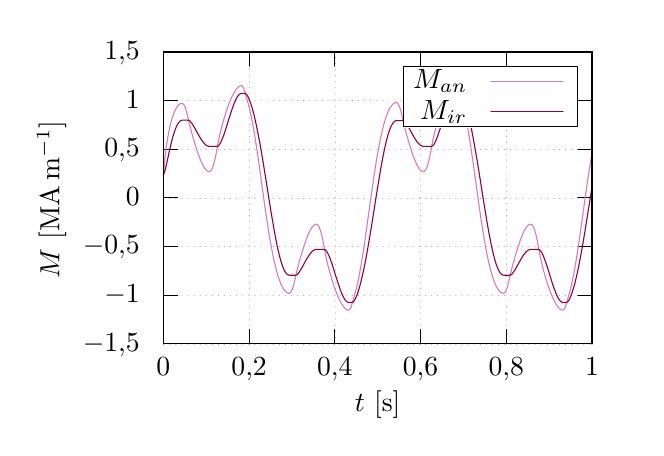
\begin{tikzpicture}[gnuplot]
%% generated with GNUPLOT 5.4p2 (Lua 5.4; terminal rev. Jun 2020, script rev. 114)
%% Fri 23 May 2025 09:04:49 AM -03
\path (0.000,0.000) rectangle (7.500,5.000);
\gpcolor{color=gp lt color axes}
\gpsetlinetype{gp lt axes}
\gpsetdashtype{gp dt axes}
\gpsetlinewidth{0.50}
\draw[gp path] (1.504,0.985)--(6.947,0.985);
\gpcolor{color=gp lt color border}
\gpsetlinetype{gp lt border}
\gpsetdashtype{gp dt solid}
\gpsetlinewidth{1.00}
\draw[gp path] (1.504,0.985)--(1.684,0.985);
\draw[gp path] (6.947,0.985)--(6.767,0.985);
\node[gp node right] at (1.320,0.985) {$-1,5$};
\gpcolor{color=gp lt color axes}
\gpsetlinetype{gp lt axes}
\gpsetdashtype{gp dt axes}
\gpsetlinewidth{0.50}
\draw[gp path] (1.504,1.603)--(6.947,1.603);
\gpcolor{color=gp lt color border}
\gpsetlinetype{gp lt border}
\gpsetdashtype{gp dt solid}
\gpsetlinewidth{1.00}
\draw[gp path] (1.504,1.603)--(1.684,1.603);
\draw[gp path] (6.947,1.603)--(6.767,1.603);
\node[gp node right] at (1.320,1.603) {$-1$};
\gpcolor{color=gp lt color axes}
\gpsetlinetype{gp lt axes}
\gpsetdashtype{gp dt axes}
\gpsetlinewidth{0.50}
\draw[gp path] (1.504,2.220)--(6.947,2.220);
\gpcolor{color=gp lt color border}
\gpsetlinetype{gp lt border}
\gpsetdashtype{gp dt solid}
\gpsetlinewidth{1.00}
\draw[gp path] (1.504,2.220)--(1.684,2.220);
\draw[gp path] (6.947,2.220)--(6.767,2.220);
\node[gp node right] at (1.320,2.220) {$-0,5$};
\gpcolor{color=gp lt color axes}
\gpsetlinetype{gp lt axes}
\gpsetdashtype{gp dt axes}
\gpsetlinewidth{0.50}
\draw[gp path] (1.504,2.838)--(6.947,2.838);
\gpcolor{color=gp lt color border}
\gpsetlinetype{gp lt border}
\gpsetdashtype{gp dt solid}
\gpsetlinewidth{1.00}
\draw[gp path] (1.504,2.838)--(1.684,2.838);
\draw[gp path] (6.947,2.838)--(6.767,2.838);
\node[gp node right] at (1.320,2.838) {$0$};
\gpcolor{color=gp lt color axes}
\gpsetlinetype{gp lt axes}
\gpsetdashtype{gp dt axes}
\gpsetlinewidth{0.50}
\draw[gp path] (1.504,3.456)--(6.947,3.456);
\gpcolor{color=gp lt color border}
\gpsetlinetype{gp lt border}
\gpsetdashtype{gp dt solid}
\gpsetlinewidth{1.00}
\draw[gp path] (1.504,3.456)--(1.684,3.456);
\draw[gp path] (6.947,3.456)--(6.767,3.456);
\node[gp node right] at (1.320,3.456) {$0,5$};
\gpcolor{color=gp lt color axes}
\gpsetlinetype{gp lt axes}
\gpsetdashtype{gp dt axes}
\gpsetlinewidth{0.50}
\draw[gp path] (1.504,4.073)--(4.559,4.073);
\draw[gp path] (6.763,4.073)--(6.947,4.073);
\gpcolor{color=gp lt color border}
\gpsetlinetype{gp lt border}
\gpsetdashtype{gp dt solid}
\gpsetlinewidth{1.00}
\draw[gp path] (1.504,4.073)--(1.684,4.073);
\draw[gp path] (6.947,4.073)--(6.767,4.073);
\node[gp node right] at (1.320,4.073) {$1$};
\gpcolor{color=gp lt color axes}
\gpsetlinetype{gp lt axes}
\gpsetdashtype{gp dt axes}
\gpsetlinewidth{0.50}
\draw[gp path] (1.504,4.691)--(6.947,4.691);
\gpcolor{color=gp lt color border}
\gpsetlinetype{gp lt border}
\gpsetdashtype{gp dt solid}
\gpsetlinewidth{1.00}
\draw[gp path] (1.504,4.691)--(1.684,4.691);
\draw[gp path] (6.947,4.691)--(6.767,4.691);
\node[gp node right] at (1.320,4.691) {$1,5$};
\gpcolor{color=gp lt color axes}
\gpsetlinetype{gp lt axes}
\gpsetdashtype{gp dt axes}
\gpsetlinewidth{0.50}
\draw[gp path] (1.504,0.985)--(1.504,4.691);
\gpcolor{color=gp lt color border}
\gpsetlinetype{gp lt border}
\gpsetdashtype{gp dt solid}
\gpsetlinewidth{1.00}
\draw[gp path] (1.504,0.985)--(1.504,1.165);
\draw[gp path] (1.504,4.691)--(1.504,4.511);
\node[gp node center] at (1.504,0.677) {$0$};
\gpcolor{color=gp lt color axes}
\gpsetlinetype{gp lt axes}
\gpsetdashtype{gp dt axes}
\gpsetlinewidth{0.50}
\draw[gp path] (2.593,0.985)--(2.593,4.691);
\gpcolor{color=gp lt color border}
\gpsetlinetype{gp lt border}
\gpsetdashtype{gp dt solid}
\gpsetlinewidth{1.00}
\draw[gp path] (2.593,0.985)--(2.593,1.165);
\draw[gp path] (2.593,4.691)--(2.593,4.511);
\node[gp node center] at (2.593,0.677) {$0,2$};
\gpcolor{color=gp lt color axes}
\gpsetlinetype{gp lt axes}
\gpsetdashtype{gp dt axes}
\gpsetlinewidth{0.50}
\draw[gp path] (3.681,0.985)--(3.681,4.691);
\gpcolor{color=gp lt color border}
\gpsetlinetype{gp lt border}
\gpsetdashtype{gp dt solid}
\gpsetlinewidth{1.00}
\draw[gp path] (3.681,0.985)--(3.681,1.165);
\draw[gp path] (3.681,4.691)--(3.681,4.511);
\node[gp node center] at (3.681,0.677) {$0,4$};
\gpcolor{color=gp lt color axes}
\gpsetlinetype{gp lt axes}
\gpsetdashtype{gp dt axes}
\gpsetlinewidth{0.50}
\draw[gp path] (4.770,0.985)--(4.770,3.741);
\draw[gp path] (4.770,4.511)--(4.770,4.691);
\gpcolor{color=gp lt color border}
\gpsetlinetype{gp lt border}
\gpsetdashtype{gp dt solid}
\gpsetlinewidth{1.00}
\draw[gp path] (4.770,0.985)--(4.770,1.165);
\draw[gp path] (4.770,4.691)--(4.770,4.511);
\node[gp node center] at (4.770,0.677) {$0,6$};
\gpcolor{color=gp lt color axes}
\gpsetlinetype{gp lt axes}
\gpsetdashtype{gp dt axes}
\gpsetlinewidth{0.50}
\draw[gp path] (5.858,0.985)--(5.858,3.741);
\draw[gp path] (5.858,4.511)--(5.858,4.691);
\gpcolor{color=gp lt color border}
\gpsetlinetype{gp lt border}
\gpsetdashtype{gp dt solid}
\gpsetlinewidth{1.00}
\draw[gp path] (5.858,0.985)--(5.858,1.165);
\draw[gp path] (5.858,4.691)--(5.858,4.511);
\node[gp node center] at (5.858,0.677) {$0,8$};
\gpcolor{color=gp lt color axes}
\gpsetlinetype{gp lt axes}
\gpsetdashtype{gp dt axes}
\gpsetlinewidth{0.50}
\draw[gp path] (6.947,0.985)--(6.947,4.691);
\gpcolor{color=gp lt color border}
\gpsetlinetype{gp lt border}
\gpsetdashtype{gp dt solid}
\gpsetlinewidth{1.00}
\draw[gp path] (6.947,0.985)--(6.947,1.165);
\draw[gp path] (6.947,4.691)--(6.947,4.511);
\node[gp node center] at (6.947,0.677) {$1$};
\draw[gp path] (1.504,4.691)--(1.504,0.985)--(6.947,0.985)--(6.947,4.691)--cycle;
\node[gp node center,rotate=-270] at (0.108,2.838) {$M$ [\si{\mega\ampere\per\meter}]};
\node[gp node center] at (4.225,0.215) {$t$ [\si{\second}]};
\draw[gp path] (4.559,3.741)--(4.559,4.511)--(6.763,4.511)--(6.763,3.741)--cycle;
\gpcolor{rgb color={0.831,0.488,0.735}}
\draw[gp path] (1.504,3.099)--(1.522,3.335)--(1.540,3.485)--(1.559,3.601)--(1.577,3.697)%
  --(1.595,3.777)--(1.613,3.844)--(1.631,3.899)--(1.650,3.944)--(1.668,3.979)--(1.686,4.006)%
  --(1.704,4.025)--(1.722,4.036)--(1.741,4.040)--(1.759,4.030)--(1.777,3.997)--(1.795,3.943)%
  --(1.813,3.871)--(1.832,3.787)--(1.850,3.717)--(1.868,3.651)--(1.886,3.588)--(1.904,3.527)%
  --(1.923,3.469)--(1.941,3.413)--(1.959,3.361)--(1.977,3.314)--(1.996,3.273)--(2.014,3.237)%
  --(2.032,3.209)--(2.050,3.188)--(2.068,3.175)--(2.087,3.171)--(2.105,3.180)--(2.123,3.210)%
  --(2.141,3.261)--(2.159,3.331)--(2.178,3.421)--(2.196,3.525)--(2.214,3.614)--(2.232,3.690)%
  --(2.250,3.761)--(2.269,3.826)--(2.287,3.887)--(2.305,3.944)--(2.323,3.996)--(2.341,4.045)%
  --(2.360,4.090)--(2.378,4.130)--(2.396,4.166)--(2.414,4.196)--(2.432,4.222)--(2.451,4.242)%
  --(2.469,4.256)--(2.487,4.263)--(2.505,4.261)--(2.523,4.233)--(2.542,4.175)--(2.560,4.110)%
  --(2.578,4.047)--(2.596,3.977)--(2.614,3.897)--(2.633,3.807)--(2.651,3.707)--(2.669,3.598)%
  --(2.687,3.481)--(2.705,3.358)--(2.724,3.230)--(2.742,3.099)--(2.760,2.967)--(2.778,2.836)%
  --(2.796,2.707)--(2.815,2.583)--(2.833,2.463)--(2.851,2.351)--(2.869,2.245)--(2.888,2.148)%
  --(2.906,2.059)--(2.924,1.979)--(2.942,1.907)--(2.960,1.844)--(2.979,1.790)--(2.997,1.744)%
  --(3.015,1.706)--(3.033,1.675)--(3.051,1.653)--(3.070,1.637)--(3.088,1.628)--(3.106,1.626)%
  --(3.124,1.642)--(3.142,1.681)--(3.161,1.739)--(3.179,1.816)--(3.197,1.901)--(3.215,1.972)%
  --(3.233,2.038)--(3.252,2.101)--(3.270,2.162)--(3.288,2.220)--(3.306,2.275)--(3.324,2.326)%
  --(3.343,2.372)--(3.361,2.412)--(3.379,2.446)--(3.397,2.472)--(3.415,2.491)--(3.434,2.502)%
  --(3.452,2.504)--(3.470,2.490)--(3.488,2.454)--(3.506,2.399)--(3.525,2.323)--(3.543,2.229)%
  --(3.561,2.126)--(3.579,2.042)--(3.597,1.967)--(3.616,1.899)--(3.634,1.835)--(3.652,1.775)%
  --(3.670,1.719)--(3.688,1.667)--(3.707,1.619)--(3.725,1.576)--(3.743,1.537)--(3.761,1.502)%
  --(3.780,1.473)--(3.798,1.448)--(3.816,1.430)--(3.834,1.418)--(3.852,1.412)--(3.871,1.420)%
  --(3.889,1.455)--(3.907,1.519)--(3.925,1.581)--(3.943,1.646)--(3.962,1.718)--(3.980,1.800)%
  --(3.998,1.893)--(4.016,1.995)--(4.034,2.106)--(4.053,2.225)--(4.071,2.350)--(4.089,2.479)%
  --(4.107,2.610)--(4.125,2.742)--(4.144,2.873)--(4.162,3.000)--(4.180,3.124)--(4.198,3.242)%
  --(4.216,3.353)--(4.235,3.456)--(4.253,3.551)--(4.271,3.638)--(4.289,3.716)--(4.307,3.785)%
  --(4.326,3.846)--(4.344,3.898)--(4.362,3.942)--(4.380,3.979)--(4.398,4.007)--(4.417,4.028)%
  --(4.435,4.042)--(4.453,4.049)--(4.471,4.048)--(4.489,4.026)--(4.508,3.983)--(4.526,3.919)%
  --(4.544,3.838)--(4.562,3.756)--(4.580,3.687)--(4.599,3.622)--(4.617,3.560)--(4.635,3.499)%
  --(4.653,3.442)--(4.671,3.388)--(4.690,3.338)--(4.708,3.294)--(4.726,3.255)--(4.744,3.223)%
  --(4.763,3.198)--(4.781,3.181)--(4.799,3.173)--(4.817,3.174)--(4.835,3.193)--(4.854,3.234)%
  --(4.872,3.294)--(4.890,3.374)--(4.908,3.473)--(4.926,3.572)--(4.945,3.653)--(4.963,3.726)%
  --(4.981,3.794)--(4.999,3.857)--(5.017,3.916)--(5.036,3.970)--(5.054,4.021)--(5.072,4.068)%
  --(5.090,4.110)--(5.108,4.148)--(5.127,4.182)--(5.145,4.210)--(5.163,4.233)--(5.181,4.250)%
  --(5.199,4.260)--(5.218,4.264)--(5.236,4.250)--(5.254,4.208)--(5.272,4.140)--(5.290,4.079)%
  --(5.309,4.013)--(5.327,3.938)--(5.345,3.853)--(5.363,3.758)--(5.381,3.654)--(5.400,3.541)%
  --(5.418,3.420)--(5.436,3.294)--(5.454,3.165)--(5.472,3.033)--(5.491,2.901)--(5.509,2.771)%
  --(5.527,2.644)--(5.545,2.522)--(5.563,2.406)--(5.582,2.297)--(5.600,2.195)--(5.618,2.102)%
  --(5.636,2.018)--(5.655,1.942)--(5.673,1.875)--(5.691,1.816)--(5.709,1.766)--(5.727,1.724)%
  --(5.746,1.690)--(5.764,1.663)--(5.782,1.644)--(5.800,1.632)--(5.818,1.626)--(5.837,1.631)%
  --(5.855,1.659)--(5.873,1.708)--(5.891,1.776)--(5.909,1.861)--(5.928,1.938)--(5.946,2.005)%
  --(5.964,2.070)--(5.982,2.132)--(6.000,2.191)--(6.019,2.248)--(6.037,2.301)--(6.055,2.349)%
  --(6.073,2.393)--(6.091,2.430)--(6.110,2.460)--(6.128,2.483)--(6.146,2.498)--(6.164,2.504)%
  --(6.182,2.499)--(6.201,2.475)--(6.219,2.429)--(6.237,2.363)--(6.255,2.279)--(6.273,2.176)%
  --(6.292,2.083)--(6.310,2.004)--(6.328,1.932)--(6.346,1.866)--(6.364,1.804)--(6.383,1.746)%
  --(6.401,1.692)--(6.419,1.643)--(6.437,1.597)--(6.455,1.556)--(6.474,1.519)--(6.492,1.487)%
  --(6.510,1.460)--(6.528,1.438)--(6.547,1.423)--(6.565,1.414)--(6.583,1.413)--(6.601,1.434)%
  --(6.619,1.484)--(6.638,1.551)--(6.656,1.613)--(6.674,1.681)--(6.692,1.758)--(6.710,1.845)%
  --(6.729,1.943)--(6.747,2.050)--(6.765,2.165)--(6.783,2.287)--(6.801,2.414)--(6.820,2.544)%
  --(6.838,2.676)--(6.856,2.808)--(6.874,2.937)--(6.892,3.063)--(6.911,3.183)--(6.929,3.298)%
  --(6.947,3.405);
\gpcolor{rgb color={0.569,0.000,0.247}}
\draw[gp path] (1.504,3.133)--(1.522,3.174)--(1.540,3.251)--(1.559,3.335)--(1.577,3.419)%
  --(1.595,3.498)--(1.613,3.572)--(1.631,3.637)--(1.650,3.694)--(1.668,3.741)--(1.686,3.777)%
  --(1.704,3.803)--(1.722,3.819)--(1.741,3.825)--(1.759,3.825)--(1.777,3.825)--(1.795,3.825)%
  --(1.813,3.825)--(1.832,3.822)--(1.850,3.806)--(1.868,3.782)--(1.886,3.753)--(1.904,3.722)%
  --(1.923,3.688)--(1.941,3.655)--(1.959,3.622)--(1.977,3.592)--(1.996,3.564)--(2.014,3.540)%
  --(2.032,3.520)--(2.050,3.505)--(2.068,3.496)--(2.087,3.492)--(2.105,3.492)--(2.123,3.492)%
  --(2.141,3.493)--(2.159,3.493)--(2.178,3.493)--(2.196,3.494)--(2.214,3.512)--(2.232,3.543)%
  --(2.250,3.583)--(2.269,3.631)--(2.287,3.684)--(2.305,3.740)--(2.323,3.799)--(2.341,3.857)%
  --(2.360,3.915)--(2.378,3.970)--(2.396,4.021)--(2.414,4.065)--(2.432,4.103)--(2.451,4.133)%
  --(2.469,4.154)--(2.487,4.164)--(2.505,4.166)--(2.523,4.166)--(2.542,4.166)--(2.560,4.154)%
  --(2.578,4.126)--(2.596,4.085)--(2.614,4.035)--(2.633,3.976)--(2.651,3.908)--(2.669,3.832)%
  --(2.687,3.749)--(2.705,3.659)--(2.724,3.563)--(2.742,3.461)--(2.760,3.355)--(2.778,3.245)%
  --(2.796,3.132)--(2.815,3.017)--(2.833,2.901)--(2.851,2.786)--(2.869,2.673)--(2.888,2.562)%
  --(2.906,2.456)--(2.924,2.356)--(2.942,2.263)--(2.960,2.178)--(2.979,2.101)--(2.997,2.035)%
  --(3.015,1.978)--(3.033,1.932)--(3.051,1.898)--(3.070,1.873)--(3.088,1.860)--(3.106,1.856)%
  --(3.124,1.856)--(3.142,1.856)--(3.161,1.856)--(3.179,1.856)--(3.197,1.860)--(3.215,1.877)%
  --(3.233,1.902)--(3.252,1.932)--(3.270,1.963)--(3.288,1.997)--(3.306,2.030)--(3.324,2.062)%
  --(3.343,2.092)--(3.361,2.119)--(3.379,2.142)--(3.397,2.161)--(3.415,2.174)--(3.434,2.182)%
  --(3.452,2.184)--(3.470,2.184)--(3.488,2.184)--(3.506,2.184)--(3.525,2.184)--(3.543,2.184)%
  --(3.561,2.179)--(3.579,2.158)--(3.597,2.124)--(3.616,2.082)--(3.634,2.033)--(3.652,1.979)%
  --(3.670,1.921)--(3.688,1.863)--(3.707,1.804)--(3.725,1.747)--(3.743,1.693)--(3.761,1.644)%
  --(3.780,1.600)--(3.798,1.565)--(3.816,1.537)--(3.834,1.519)--(3.852,1.511)--(3.871,1.510)%
  --(3.889,1.510)--(3.907,1.511)--(3.925,1.528)--(3.943,1.559)--(3.962,1.602)--(3.980,1.655)%
  --(3.998,1.717)--(4.016,1.786)--(4.034,1.864)--(4.053,1.949)--(4.071,2.041)--(4.089,2.138)%
  --(4.107,2.241)--(4.125,2.348)--(4.144,2.459)--(4.162,2.573)--(4.180,2.688)--(4.198,2.804)%
  --(4.216,2.919)--(4.235,3.031)--(4.253,3.141)--(4.271,3.245)--(4.289,3.344)--(4.307,3.435)%
  --(4.326,3.518)--(4.344,3.592)--(4.362,3.657)--(4.380,3.710)--(4.398,3.753)--(4.417,3.785)%
  --(4.435,3.807)--(4.453,3.818)--(4.471,3.820)--(4.489,3.820)--(4.508,3.820)--(4.526,3.820)%
  --(4.544,3.820)--(4.562,3.813)--(4.580,3.793)--(4.599,3.767)--(4.617,3.737)--(4.635,3.704)%
  --(4.653,3.671)--(4.671,3.638)--(4.690,3.606)--(4.708,3.577)--(4.726,3.551)--(4.744,3.529)%
  --(4.763,3.511)--(4.781,3.499)--(4.799,3.493)--(4.817,3.492)--(4.835,3.492)--(4.854,3.492)%
  --(4.872,3.492)--(4.890,3.492)--(4.908,3.492)--(4.926,3.501)--(4.945,3.526)--(4.963,3.562)%
  --(4.981,3.606)--(4.999,3.657)--(5.017,3.711)--(5.036,3.769)--(5.054,3.828)--(5.072,3.887)%
  --(5.090,3.943)--(5.108,3.996)--(5.127,4.044)--(5.145,4.085)--(5.163,4.119)--(5.181,4.144)%
  --(5.199,4.160)--(5.218,4.166)--(5.236,4.166)--(5.254,4.166)--(5.272,4.163)--(5.290,4.141)%
  --(5.309,4.107)--(5.327,4.061)--(5.345,4.007)--(5.363,3.943)--(5.381,3.871)--(5.400,3.791)%
  --(5.418,3.705)--(5.436,3.611)--(5.454,3.513)--(5.472,3.408)--(5.491,3.300)--(5.509,3.188)%
  --(5.527,3.074)--(5.545,2.959)--(5.563,2.843)--(5.582,2.729)--(5.600,2.617)--(5.618,2.509)%
  --(5.636,2.406)--(5.655,2.309)--(5.673,2.219)--(5.691,2.138)--(5.709,2.067)--(5.727,2.005)%
  --(5.746,1.954)--(5.764,1.914)--(5.782,1.884)--(5.800,1.865)--(5.818,1.857)--(5.837,1.856)%
  --(5.855,1.856)--(5.873,1.856)--(5.891,1.856)--(5.909,1.856)--(5.928,1.868)--(5.946,1.889)%
  --(5.964,1.917)--(5.982,1.947)--(6.000,1.980)--(6.019,2.013)--(6.037,2.046)--(6.055,2.077)%
  --(6.073,2.106)--(6.091,2.131)--(6.110,2.152)--(6.128,2.168)--(6.146,2.179)--(6.164,2.184)%
  --(6.182,2.184)--(6.201,2.184)--(6.219,2.184)--(6.237,2.184)--(6.255,2.184)--(6.273,2.184)%
  --(6.292,2.170)--(6.310,2.142)--(6.328,2.104)--(6.346,2.058)--(6.364,2.006)--(6.383,1.950)%
  --(6.401,1.892)--(6.419,1.833)--(6.437,1.775)--(6.455,1.719)--(6.474,1.668)--(6.492,1.621)%
  --(6.510,1.582)--(6.528,1.550)--(6.547,1.527)--(6.565,1.513)--(6.583,1.510)--(6.601,1.510)%
  --(6.619,1.510)--(6.638,1.517)--(6.656,1.542)--(6.674,1.580)--(6.692,1.627)--(6.710,1.685)%
  --(6.729,1.750)--(6.747,1.824)--(6.765,1.906)--(6.783,1.994)--(6.801,2.089)--(6.820,2.189)%
  --(6.838,2.294)--(6.856,2.404)--(6.874,2.516)--(6.892,2.630)--(6.911,2.746)--(6.929,2.861)%
  --(6.947,2.975);
\gpfill{color=gpbgfillcolor} (4.559,3.741)--(6.763,3.741)--(6.763,4.511)--(4.559,4.511)--cycle;
\gpcolor{color=gp lt color border}
\draw[gp path] (4.559,3.741)--(4.559,4.511)--(6.763,4.511)--(6.763,3.741)--cycle;
\node[gp node right] at (5.479,4.318) {\phantom{M}$M_{an}$};
\gpcolor{rgb color={0.831,0.488,0.735}}
\draw[gp path] (5.663,4.318)--(6.579,4.318);
\gpcolor{color=gp lt color border}
\node[gp node right] at (5.479,3.933) {\phantom{M}$M_{ir}$};
\gpcolor{rgb color={0.569,0.000,0.247}}
\draw[gp path] (5.663,3.933)--(6.579,3.933);
\gpcolor{color=gp lt color border}
\draw[gp path] (1.504,4.691)--(1.504,0.985)--(6.947,0.985)--(6.947,4.691)--cycle;
%% coordinates of the plot area
\gpdefrectangularnode{gp plot 1}{\pgfpoint{1.504cm}{0.985cm}}{\pgfpoint{6.947cm}{4.691cm}}
\end{tikzpicture}
%% gnuplot variables

    \vspace{-1cm}
    \caption{HHHHHHHHHHHHHHH}
  \end{minipage}%
\end{figure}

\newpage

\begin{figure}[!h]
  \begin{minipage}{.49\linewidth}
    \centering
    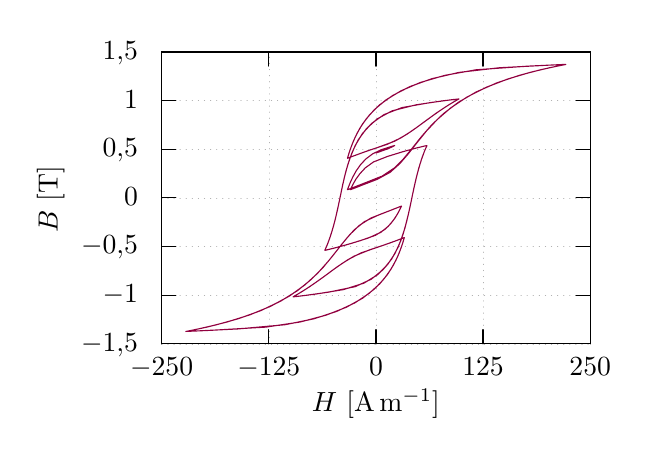
\begin{tikzpicture}[gnuplot]
%% generated with GNUPLOT 5.4p2 (Lua 5.4; terminal rev. Jun 2020, script rev. 114)
%% Fri 23 May 2025 09:04:29 AM -03
\path (0.000,0.000) rectangle (7.500,5.000);
\gpcolor{color=gp lt color axes}
\gpsetlinetype{gp lt axes}
\gpsetdashtype{gp dt axes}
\gpsetlinewidth{0.50}
\draw[gp path] (1.504,0.985)--(6.947,0.985);
\gpcolor{color=gp lt color border}
\gpsetlinetype{gp lt border}
\gpsetdashtype{gp dt solid}
\gpsetlinewidth{1.00}
\draw[gp path] (1.504,0.985)--(1.684,0.985);
\draw[gp path] (6.947,0.985)--(6.767,0.985);
\node[gp node right] at (1.320,0.985) {$-1,5$};
\gpcolor{color=gp lt color axes}
\gpsetlinetype{gp lt axes}
\gpsetdashtype{gp dt axes}
\gpsetlinewidth{0.50}
\draw[gp path] (1.504,1.603)--(6.947,1.603);
\gpcolor{color=gp lt color border}
\gpsetlinetype{gp lt border}
\gpsetdashtype{gp dt solid}
\gpsetlinewidth{1.00}
\draw[gp path] (1.504,1.603)--(1.684,1.603);
\draw[gp path] (6.947,1.603)--(6.767,1.603);
\node[gp node right] at (1.320,1.603) {$-1$};
\gpcolor{color=gp lt color axes}
\gpsetlinetype{gp lt axes}
\gpsetdashtype{gp dt axes}
\gpsetlinewidth{0.50}
\draw[gp path] (1.504,2.220)--(6.947,2.220);
\gpcolor{color=gp lt color border}
\gpsetlinetype{gp lt border}
\gpsetdashtype{gp dt solid}
\gpsetlinewidth{1.00}
\draw[gp path] (1.504,2.220)--(1.684,2.220);
\draw[gp path] (6.947,2.220)--(6.767,2.220);
\node[gp node right] at (1.320,2.220) {$-0,5$};
\gpcolor{color=gp lt color axes}
\gpsetlinetype{gp lt axes}
\gpsetdashtype{gp dt axes}
\gpsetlinewidth{0.50}
\draw[gp path] (1.504,2.838)--(6.947,2.838);
\gpcolor{color=gp lt color border}
\gpsetlinetype{gp lt border}
\gpsetdashtype{gp dt solid}
\gpsetlinewidth{1.00}
\draw[gp path] (1.504,2.838)--(1.684,2.838);
\draw[gp path] (6.947,2.838)--(6.767,2.838);
\node[gp node right] at (1.320,2.838) {$0$};
\gpcolor{color=gp lt color axes}
\gpsetlinetype{gp lt axes}
\gpsetdashtype{gp dt axes}
\gpsetlinewidth{0.50}
\draw[gp path] (1.504,3.456)--(6.947,3.456);
\gpcolor{color=gp lt color border}
\gpsetlinetype{gp lt border}
\gpsetdashtype{gp dt solid}
\gpsetlinewidth{1.00}
\draw[gp path] (1.504,3.456)--(1.684,3.456);
\draw[gp path] (6.947,3.456)--(6.767,3.456);
\node[gp node right] at (1.320,3.456) {$0,5$};
\gpcolor{color=gp lt color axes}
\gpsetlinetype{gp lt axes}
\gpsetdashtype{gp dt axes}
\gpsetlinewidth{0.50}
\draw[gp path] (1.504,4.073)--(6.947,4.073);
\gpcolor{color=gp lt color border}
\gpsetlinetype{gp lt border}
\gpsetdashtype{gp dt solid}
\gpsetlinewidth{1.00}
\draw[gp path] (1.504,4.073)--(1.684,4.073);
\draw[gp path] (6.947,4.073)--(6.767,4.073);
\node[gp node right] at (1.320,4.073) {$1$};
\gpcolor{color=gp lt color axes}
\gpsetlinetype{gp lt axes}
\gpsetdashtype{gp dt axes}
\gpsetlinewidth{0.50}
\draw[gp path] (1.504,4.691)--(6.947,4.691);
\gpcolor{color=gp lt color border}
\gpsetlinetype{gp lt border}
\gpsetdashtype{gp dt solid}
\gpsetlinewidth{1.00}
\draw[gp path] (1.504,4.691)--(1.684,4.691);
\draw[gp path] (6.947,4.691)--(6.767,4.691);
\node[gp node right] at (1.320,4.691) {$1,5$};
\gpcolor{color=gp lt color axes}
\gpsetlinetype{gp lt axes}
\gpsetdashtype{gp dt axes}
\gpsetlinewidth{0.50}
\draw[gp path] (1.504,0.985)--(1.504,4.691);
\gpcolor{color=gp lt color border}
\gpsetlinetype{gp lt border}
\gpsetdashtype{gp dt solid}
\gpsetlinewidth{1.00}
\draw[gp path] (1.504,0.985)--(1.504,1.165);
\draw[gp path] (1.504,4.691)--(1.504,4.511);
\node[gp node center] at (1.504,0.677) {$-250$};
\gpcolor{color=gp lt color axes}
\gpsetlinetype{gp lt axes}
\gpsetdashtype{gp dt axes}
\gpsetlinewidth{0.50}
\draw[gp path] (2.865,0.985)--(2.865,4.691);
\gpcolor{color=gp lt color border}
\gpsetlinetype{gp lt border}
\gpsetdashtype{gp dt solid}
\gpsetlinewidth{1.00}
\draw[gp path] (2.865,0.985)--(2.865,1.165);
\draw[gp path] (2.865,4.691)--(2.865,4.511);
\node[gp node center] at (2.865,0.677) {$-125$};
\gpcolor{color=gp lt color axes}
\gpsetlinetype{gp lt axes}
\gpsetdashtype{gp dt axes}
\gpsetlinewidth{0.50}
\draw[gp path] (4.226,0.985)--(4.226,4.691);
\gpcolor{color=gp lt color border}
\gpsetlinetype{gp lt border}
\gpsetdashtype{gp dt solid}
\gpsetlinewidth{1.00}
\draw[gp path] (4.226,0.985)--(4.226,1.165);
\draw[gp path] (4.226,4.691)--(4.226,4.511);
\node[gp node center] at (4.226,0.677) {$0$};
\gpcolor{color=gp lt color axes}
\gpsetlinetype{gp lt axes}
\gpsetdashtype{gp dt axes}
\gpsetlinewidth{0.50}
\draw[gp path] (5.586,0.985)--(5.586,4.691);
\gpcolor{color=gp lt color border}
\gpsetlinetype{gp lt border}
\gpsetdashtype{gp dt solid}
\gpsetlinewidth{1.00}
\draw[gp path] (5.586,0.985)--(5.586,1.165);
\draw[gp path] (5.586,4.691)--(5.586,4.511);
\node[gp node center] at (5.586,0.677) {$125$};
\gpcolor{color=gp lt color axes}
\gpsetlinetype{gp lt axes}
\gpsetdashtype{gp dt axes}
\gpsetlinewidth{0.50}
\draw[gp path] (6.947,0.985)--(6.947,4.691);
\gpcolor{color=gp lt color border}
\gpsetlinetype{gp lt border}
\gpsetdashtype{gp dt solid}
\gpsetlinewidth{1.00}
\draw[gp path] (6.947,0.985)--(6.947,1.165);
\draw[gp path] (6.947,4.691)--(6.947,4.511);
\node[gp node center] at (6.947,0.677) {$250$};
\draw[gp path] (1.504,4.691)--(1.504,0.985)--(6.947,0.985)--(6.947,4.691)--cycle;
\node[gp node center,rotate=-270] at (0.108,2.838) {$B$ [\si{\tesla}]};
\node[gp node center] at (4.225,0.215) {$H$ [\si{\ampere\per\meter}]};
\gpcolor{rgb color={0.569,0.000,0.247}}
\draw[gp path] (4.226,3.408)--(4.387,3.465)--(4.453,3.497)--(4.464,3.504)--(4.409,3.487)%
  --(4.293,3.450)--(4.183,3.397)--(4.096,3.331)--(4.028,3.257)--(3.975,3.181)--(3.935,3.109)%
  --(3.904,3.044)--(3.883,2.992)--(3.869,2.957)--(3.864,2.942)--(3.884,2.949)--(3.965,2.981)%
  --(4.108,3.037)--(4.307,3.116)--(4.457,3.216)--(4.576,3.335)--(4.686,3.468)--(4.800,3.612)%
  --(4.929,3.760)--(5.083,3.908)--(5.271,4.051)--(5.496,4.182)--(5.759,4.298)--(6.044,4.394)%
  --(6.319,4.466)--(6.535,4.513)--(6.637,4.533)--(6.442,4.525)--(5.792,4.491)--(5.281,4.432)%
  --(4.936,4.352)--(4.660,4.253)--(4.442,4.141)--(4.274,4.021)--(4.148,3.897)--(4.055,3.776)%
  --(3.988,3.662)--(3.940,3.560)--(3.907,3.474)--(3.884,3.408)--(3.871,3.364)--(3.865,3.343)%
  --(3.876,3.346)--(3.942,3.371)--(4.067,3.417)--(4.252,3.480)--(4.464,3.558)--(4.617,3.645)%
  --(4.748,3.736)--(4.871,3.827)--(4.988,3.912)--(5.097,3.985)--(5.189,4.043)--(5.253,4.080)%
  --(5.280,4.095)--(5.189,4.085)--(4.913,4.048)--(4.556,3.985)--(4.328,3.896)--(4.170,3.783)%
  --(4.051,3.651)--(3.962,3.502)--(3.895,3.342)--(3.844,3.175)--(3.804,3.007)--(3.770,2.843)%
  --(3.738,2.689)--(3.705,2.549)--(3.671,2.427)--(3.639,2.327)--(3.611,2.251)--(3.589,2.200)%
  --(3.578,2.175)--(3.588,2.174)--(3.679,2.196)--(3.836,2.238)--(4.027,2.295)--(4.220,2.363)%
  --(4.339,2.438)--(4.415,2.513)--(4.469,2.584)--(4.506,2.646)--(4.532,2.695)--(4.546,2.725)%
  --(4.551,2.734)--(4.516,2.721)--(4.419,2.683)--(4.261,2.622)--(4.080,2.537)--(3.950,2.432)%
  --(3.840,2.309)--(3.732,2.173)--(3.616,2.028)--(3.483,1.879)--(3.322,1.732)--(3.126,1.591)%
  --(2.891,1.463)--(2.622,1.352)--(2.335,1.262)--(2.070,1.195)--(1.878,1.155)--(1.811,1.142)%
  --(2.143,1.157)--(2.827,1.197)--(3.264,1.262)--(3.590,1.348)--(3.851,1.450)--(4.056,1.564)%
  --(4.212,1.686)--(4.329,1.810)--(4.415,1.930)--(4.477,2.041)--(4.521,2.139)--(4.551,2.220)%
  --(4.571,2.281)--(4.582,2.319)--(4.586,2.334)--(4.564,2.326)--(4.483,2.295)--(4.344,2.245)%
  --(4.142,2.177)--(3.945,2.097)--(3.800,2.008)--(3.671,1.917)--(3.550,1.827)--(3.434,1.745)%
  --(3.329,1.675)--(3.243,1.622)--(3.187,1.590)--(3.174,1.581)--(3.317,1.598)--(3.625,1.641)%
  --(3.963,1.711)--(4.167,1.806)--(4.314,1.924)--(4.425,2.061)--(4.508,2.213)--(4.570,2.375)%
  --(4.617,2.543)--(4.656,2.711)--(4.689,2.872)--(4.722,3.024)--(4.755,3.159)--(4.788,3.276)%
  --(4.819,3.370)--(4.846,3.440)--(4.865,3.484)--(4.874,3.503)--(4.848,3.498)--(4.737,3.471)%
  --(4.569,3.425)--(4.374,3.365)--(4.195,3.295)--(4.090,3.219)--(4.021,3.144)--(3.971,3.075)%
  --(3.937,3.016)--(3.915,2.972)--(3.902,2.947)--(3.903,2.943)--(3.954,2.962)--(4.065,3.006)%
  --(4.240,3.073)--(4.406,3.163)--(4.529,3.273)--(4.638,3.400)--(4.747,3.539)--(4.866,3.686)%
  --(5.005,3.834)--(5.174,3.980)--(5.380,4.118)--(5.624,4.242)--(5.900,4.348)--(6.186,4.433)%
  --(6.438,4.493)--(6.603,4.526)--(6.614,4.533)--(6.150,4.511)--(5.496,4.465)--(5.098,4.394)%
  --(4.790,4.304)--(4.544,4.198)--(4.352,4.082)--(4.206,3.959)--(4.098,3.836)--(4.019,3.718)%
  --(3.962,3.609)--(3.922,3.515)--(3.894,3.439)--(3.877,3.383)--(3.867,3.351)--(3.865,3.341)%
  --(3.902,3.356)--(3.997,3.391)--(4.152,3.447)--(4.368,3.518)--(4.545,3.601)--(4.684,3.690)%
  --(4.811,3.782)--(4.931,3.870)--(5.044,3.950)--(5.145,4.016)--(5.225,4.064)--(5.272,4.091)%
  --(5.261,4.093)--(5.069,4.070)--(4.734,4.020)--(4.429,3.943)--(4.243,3.842)--(4.107,3.720)%
  --(4.003,3.578)--(3.926,3.423)--(3.868,3.259)--(3.823,3.091)--(3.787,2.924)--(3.754,2.765)%
  --(3.721,2.617)--(3.688,2.485)--(3.655,2.374)--(3.624,2.286)--(3.599,2.223)--(3.582,2.185)%
  --(3.577,2.172)--(3.623,2.183)--(3.751,2.215)--(3.929,2.265)--(4.128,2.328)--(4.287,2.400)%
  --(4.381,2.476)--(4.444,2.550)--(4.489,2.617)--(4.521,2.673)--(4.540,2.712)--(4.550,2.733)%
  --(4.541,2.731)--(4.475,2.705)--(4.348,2.655)--(4.161,2.582)--(4.012,2.487)--(3.894,2.372)%
  --(3.786,2.242)--(3.676,2.101)--(3.553,1.953)--(3.407,1.805)--(3.229,1.660)--(3.014,1.526)%
  --(2.760,1.405)--(2.479,1.304)--(2.197,1.226)--(1.961,1.172)--(1.827,1.145)--(1.905,1.146)%
  --(2.475,1.174)--(3.068,1.227)--(3.437,1.302)--(3.728,1.397)--(3.960,1.506)--(4.139,1.625)%
  --(4.275,1.748)--(4.376,1.870)--(4.449,1.987)--(4.501,2.092)--(4.537,2.182)--(4.562,2.253)%
  --(4.577,2.303)--(4.585,2.330)--(4.582,2.333)--(4.531,2.313)--(4.421,2.272)--(4.251,2.213)%
  --(4.032,2.138)--(3.869,2.053)--(3.734,1.963)--(3.610,1.871)--(3.491,1.785)--(3.380,1.708)%
  --(3.283,1.646)--(3.211,1.603)--(3.174,1.582)--(3.220,1.586)--(3.457,1.616)--(3.812,1.673)%
  --(4.075,1.756)--(4.246,1.862)--(4.373,1.990)--(4.469,2.135)--(4.541,2.293)--(4.595,2.459)%
  --(4.637,2.627)--(4.673,2.793)--(4.705,2.950)--(4.738,3.094)--(4.771,3.220)--(4.804,3.326)%
  --(4.834,3.408);
\gpcolor{color=gp lt color border}
\draw[gp path] (1.504,4.691)--(1.504,0.985)--(6.947,0.985)--(6.947,4.691)--cycle;
%% coordinates of the plot area
\gpdefrectangularnode{gp plot 1}{\pgfpoint{1.504cm}{0.985cm}}{\pgfpoint{6.947cm}{4.691cm}}
\end{tikzpicture}
%% gnuplot variables

    \vspace{-1cm}
    \caption{uma caption}
  \end{minipage}%
  \begin{minipage}{.49\linewidth}
    \centering
    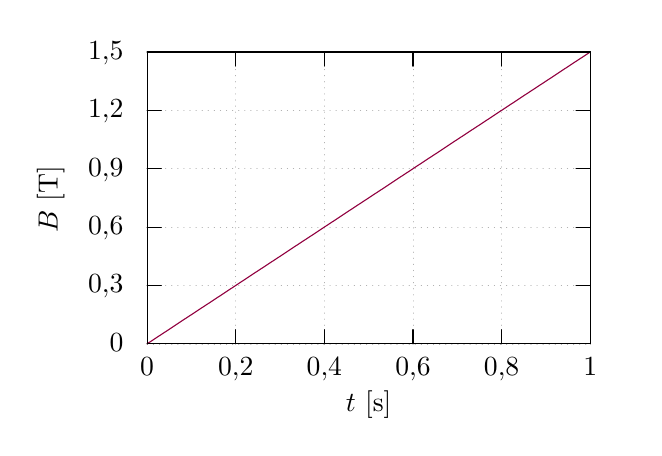
\begin{tikzpicture}[gnuplot]
%% generated with GNUPLOT 5.4p2 (Lua 5.4; terminal rev. Jun 2020, script rev. 114)
%% Fri 23 May 2025 09:06:32 AM -03
\path (0.000,0.000) rectangle (7.500,5.000);
\gpcolor{color=gp lt color axes}
\gpsetlinetype{gp lt axes}
\gpsetdashtype{gp dt axes}
\gpsetlinewidth{0.50}
\draw[gp path] (1.320,0.985)--(6.947,0.985);
\gpcolor{color=gp lt color border}
\gpsetlinetype{gp lt border}
\gpsetdashtype{gp dt solid}
\gpsetlinewidth{1.00}
\draw[gp path] (1.320,0.985)--(1.500,0.985);
\draw[gp path] (6.947,0.985)--(6.767,0.985);
\node[gp node right] at (1.136,0.985) {$0$};
\gpcolor{color=gp lt color axes}
\gpsetlinetype{gp lt axes}
\gpsetdashtype{gp dt axes}
\gpsetlinewidth{0.50}
\draw[gp path] (1.320,1.726)--(6.947,1.726);
\gpcolor{color=gp lt color border}
\gpsetlinetype{gp lt border}
\gpsetdashtype{gp dt solid}
\gpsetlinewidth{1.00}
\draw[gp path] (1.320,1.726)--(1.500,1.726);
\draw[gp path] (6.947,1.726)--(6.767,1.726);
\node[gp node right] at (1.136,1.726) {$0,3$};
\gpcolor{color=gp lt color axes}
\gpsetlinetype{gp lt axes}
\gpsetdashtype{gp dt axes}
\gpsetlinewidth{0.50}
\draw[gp path] (1.320,2.467)--(6.947,2.467);
\gpcolor{color=gp lt color border}
\gpsetlinetype{gp lt border}
\gpsetdashtype{gp dt solid}
\gpsetlinewidth{1.00}
\draw[gp path] (1.320,2.467)--(1.500,2.467);
\draw[gp path] (6.947,2.467)--(6.767,2.467);
\node[gp node right] at (1.136,2.467) {$0,6$};
\gpcolor{color=gp lt color axes}
\gpsetlinetype{gp lt axes}
\gpsetdashtype{gp dt axes}
\gpsetlinewidth{0.50}
\draw[gp path] (1.320,3.209)--(6.947,3.209);
\gpcolor{color=gp lt color border}
\gpsetlinetype{gp lt border}
\gpsetdashtype{gp dt solid}
\gpsetlinewidth{1.00}
\draw[gp path] (1.320,3.209)--(1.500,3.209);
\draw[gp path] (6.947,3.209)--(6.767,3.209);
\node[gp node right] at (1.136,3.209) {$0,9$};
\gpcolor{color=gp lt color axes}
\gpsetlinetype{gp lt axes}
\gpsetdashtype{gp dt axes}
\gpsetlinewidth{0.50}
\draw[gp path] (1.320,3.950)--(6.947,3.950);
\gpcolor{color=gp lt color border}
\gpsetlinetype{gp lt border}
\gpsetdashtype{gp dt solid}
\gpsetlinewidth{1.00}
\draw[gp path] (1.320,3.950)--(1.500,3.950);
\draw[gp path] (6.947,3.950)--(6.767,3.950);
\node[gp node right] at (1.136,3.950) {$1,2$};
\gpcolor{color=gp lt color axes}
\gpsetlinetype{gp lt axes}
\gpsetdashtype{gp dt axes}
\gpsetlinewidth{0.50}
\draw[gp path] (1.320,4.691)--(6.947,4.691);
\gpcolor{color=gp lt color border}
\gpsetlinetype{gp lt border}
\gpsetdashtype{gp dt solid}
\gpsetlinewidth{1.00}
\draw[gp path] (1.320,4.691)--(1.500,4.691);
\draw[gp path] (6.947,4.691)--(6.767,4.691);
\node[gp node right] at (1.136,4.691) {$1,5$};
\gpcolor{color=gp lt color axes}
\gpsetlinetype{gp lt axes}
\gpsetdashtype{gp dt axes}
\gpsetlinewidth{0.50}
\draw[gp path] (1.320,0.985)--(1.320,4.691);
\gpcolor{color=gp lt color border}
\gpsetlinetype{gp lt border}
\gpsetdashtype{gp dt solid}
\gpsetlinewidth{1.00}
\draw[gp path] (1.320,0.985)--(1.320,1.165);
\draw[gp path] (1.320,4.691)--(1.320,4.511);
\node[gp node center] at (1.320,0.677) {$0$};
\gpcolor{color=gp lt color axes}
\gpsetlinetype{gp lt axes}
\gpsetdashtype{gp dt axes}
\gpsetlinewidth{0.50}
\draw[gp path] (2.445,0.985)--(2.445,4.691);
\gpcolor{color=gp lt color border}
\gpsetlinetype{gp lt border}
\gpsetdashtype{gp dt solid}
\gpsetlinewidth{1.00}
\draw[gp path] (2.445,0.985)--(2.445,1.165);
\draw[gp path] (2.445,4.691)--(2.445,4.511);
\node[gp node center] at (2.445,0.677) {$0,2$};
\gpcolor{color=gp lt color axes}
\gpsetlinetype{gp lt axes}
\gpsetdashtype{gp dt axes}
\gpsetlinewidth{0.50}
\draw[gp path] (3.571,0.985)--(3.571,4.691);
\gpcolor{color=gp lt color border}
\gpsetlinetype{gp lt border}
\gpsetdashtype{gp dt solid}
\gpsetlinewidth{1.00}
\draw[gp path] (3.571,0.985)--(3.571,1.165);
\draw[gp path] (3.571,4.691)--(3.571,4.511);
\node[gp node center] at (3.571,0.677) {$0,4$};
\gpcolor{color=gp lt color axes}
\gpsetlinetype{gp lt axes}
\gpsetdashtype{gp dt axes}
\gpsetlinewidth{0.50}
\draw[gp path] (4.696,0.985)--(4.696,4.691);
\gpcolor{color=gp lt color border}
\gpsetlinetype{gp lt border}
\gpsetdashtype{gp dt solid}
\gpsetlinewidth{1.00}
\draw[gp path] (4.696,0.985)--(4.696,1.165);
\draw[gp path] (4.696,4.691)--(4.696,4.511);
\node[gp node center] at (4.696,0.677) {$0,6$};
\gpcolor{color=gp lt color axes}
\gpsetlinetype{gp lt axes}
\gpsetdashtype{gp dt axes}
\gpsetlinewidth{0.50}
\draw[gp path] (5.822,0.985)--(5.822,4.691);
\gpcolor{color=gp lt color border}
\gpsetlinetype{gp lt border}
\gpsetdashtype{gp dt solid}
\gpsetlinewidth{1.00}
\draw[gp path] (5.822,0.985)--(5.822,1.165);
\draw[gp path] (5.822,4.691)--(5.822,4.511);
\node[gp node center] at (5.822,0.677) {$0,8$};
\gpcolor{color=gp lt color axes}
\gpsetlinetype{gp lt axes}
\gpsetdashtype{gp dt axes}
\gpsetlinewidth{0.50}
\draw[gp path] (6.947,0.985)--(6.947,4.691);
\gpcolor{color=gp lt color border}
\gpsetlinetype{gp lt border}
\gpsetdashtype{gp dt solid}
\gpsetlinewidth{1.00}
\draw[gp path] (6.947,0.985)--(6.947,1.165);
\draw[gp path] (6.947,4.691)--(6.947,4.511);
\node[gp node center] at (6.947,0.677) {$1$};
\draw[gp path] (1.320,4.691)--(1.320,0.985)--(6.947,0.985)--(6.947,4.691)--cycle;
\node[gp node center,rotate=-270] at (0.108,2.838) {$B$ [\si{\tesla}]};
\node[gp node center] at (4.133,0.215) {$t$ [\si{\second}]};
\gpcolor{rgb color={0.569,0.000,0.247}}
\draw[gp path] (1.320,0.985)--(1.435,1.061)--(1.550,1.136)--(1.665,1.212)--(1.779,1.288)%
  --(1.894,1.363)--(2.009,1.439)--(2.124,1.514)--(2.239,1.590)--(2.354,1.666)--(2.468,1.741)%
  --(2.583,1.817)--(2.698,1.893)--(2.813,1.968)--(2.928,2.044)--(3.043,2.119)--(3.157,2.195)%
  --(3.272,2.271)--(3.387,2.346)--(3.502,2.422)--(3.617,2.498)--(3.732,2.573)--(3.846,2.649)%
  --(3.961,2.725)--(4.076,2.800)--(4.191,2.876)--(4.306,2.951)--(4.421,3.027)--(4.535,3.103)%
  --(4.650,3.178)--(4.765,3.254)--(4.880,3.330)--(4.995,3.405)--(5.110,3.481)--(5.224,3.557)%
  --(5.339,3.632)--(5.454,3.708)--(5.569,3.783)--(5.684,3.859)--(5.799,3.935)--(5.913,4.010)%
  --(6.028,4.086)--(6.143,4.162)--(6.258,4.237)--(6.373,4.313)--(6.488,4.388)--(6.602,4.464)%
  --(6.717,4.540)--(6.832,4.615)--(6.947,4.691);
\gpcolor{color=gp lt color border}
\draw[gp path] (1.320,4.691)--(1.320,0.985)--(6.947,0.985)--(6.947,4.691)--cycle;
%% coordinates of the plot area
\gpdefrectangularnode{gp plot 1}{\pgfpoint{1.320cm}{0.985cm}}{\pgfpoint{6.947cm}{4.691cm}}
\end{tikzpicture}
%% gnuplot variables

    \vspace{-1cm}
    \caption{HHHHHHHHHHHHHHH}
  \end{minipage}
  \begin{minipage}{.49\linewidth}
    \centering
    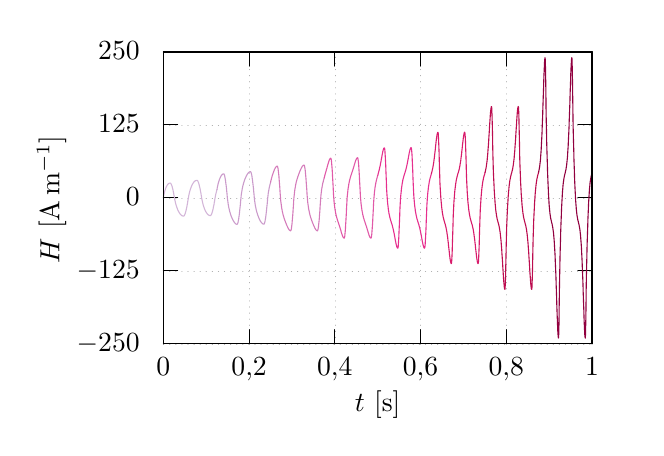
\begin{tikzpicture}[gnuplot]
%% generated with GNUPLOT 5.4p2 (Lua 5.4; terminal rev. Jun 2020, script rev. 114)
%% Fri 23 May 2025 09:05:47 AM -03
\path (0.000,0.000) rectangle (7.500,5.000);
\gpcolor{color=gp lt color axes}
\gpsetlinetype{gp lt axes}
\gpsetdashtype{gp dt axes}
\gpsetlinewidth{0.50}
\draw[gp path] (1.504,0.985)--(6.947,0.985);
\gpcolor{color=gp lt color border}
\gpsetlinetype{gp lt border}
\gpsetdashtype{gp dt solid}
\gpsetlinewidth{1.00}
\draw[gp path] (1.504,0.985)--(1.684,0.985);
\draw[gp path] (6.947,0.985)--(6.767,0.985);
\node[gp node right] at (1.320,0.985) {$-250$};
\gpcolor{color=gp lt color axes}
\gpsetlinetype{gp lt axes}
\gpsetdashtype{gp dt axes}
\gpsetlinewidth{0.50}
\draw[gp path] (1.504,1.912)--(6.947,1.912);
\gpcolor{color=gp lt color border}
\gpsetlinetype{gp lt border}
\gpsetdashtype{gp dt solid}
\gpsetlinewidth{1.00}
\draw[gp path] (1.504,1.912)--(1.684,1.912);
\draw[gp path] (6.947,1.912)--(6.767,1.912);
\node[gp node right] at (1.320,1.912) {$-125$};
\gpcolor{color=gp lt color axes}
\gpsetlinetype{gp lt axes}
\gpsetdashtype{gp dt axes}
\gpsetlinewidth{0.50}
\draw[gp path] (1.504,2.838)--(6.947,2.838);
\gpcolor{color=gp lt color border}
\gpsetlinetype{gp lt border}
\gpsetdashtype{gp dt solid}
\gpsetlinewidth{1.00}
\draw[gp path] (1.504,2.838)--(1.684,2.838);
\draw[gp path] (6.947,2.838)--(6.767,2.838);
\node[gp node right] at (1.320,2.838) {$0$};
\gpcolor{color=gp lt color axes}
\gpsetlinetype{gp lt axes}
\gpsetdashtype{gp dt axes}
\gpsetlinewidth{0.50}
\draw[gp path] (1.504,3.765)--(6.947,3.765);
\gpcolor{color=gp lt color border}
\gpsetlinetype{gp lt border}
\gpsetdashtype{gp dt solid}
\gpsetlinewidth{1.00}
\draw[gp path] (1.504,3.765)--(1.684,3.765);
\draw[gp path] (6.947,3.765)--(6.767,3.765);
\node[gp node right] at (1.320,3.765) {$125$};
\gpcolor{color=gp lt color axes}
\gpsetlinetype{gp lt axes}
\gpsetdashtype{gp dt axes}
\gpsetlinewidth{0.50}
\draw[gp path] (1.504,4.691)--(6.947,4.691);
\gpcolor{color=gp lt color border}
\gpsetlinetype{gp lt border}
\gpsetdashtype{gp dt solid}
\gpsetlinewidth{1.00}
\draw[gp path] (1.504,4.691)--(1.684,4.691);
\draw[gp path] (6.947,4.691)--(6.767,4.691);
\node[gp node right] at (1.320,4.691) {$250$};
\gpcolor{color=gp lt color axes}
\gpsetlinetype{gp lt axes}
\gpsetdashtype{gp dt axes}
\gpsetlinewidth{0.50}
\draw[gp path] (1.504,0.985)--(1.504,4.691);
\gpcolor{color=gp lt color border}
\gpsetlinetype{gp lt border}
\gpsetdashtype{gp dt solid}
\gpsetlinewidth{1.00}
\draw[gp path] (1.504,0.985)--(1.504,1.165);
\draw[gp path] (1.504,4.691)--(1.504,4.511);
\node[gp node center] at (1.504,0.677) {$0$};
\gpcolor{color=gp lt color axes}
\gpsetlinetype{gp lt axes}
\gpsetdashtype{gp dt axes}
\gpsetlinewidth{0.50}
\draw[gp path] (2.593,0.985)--(2.593,4.691);
\gpcolor{color=gp lt color border}
\gpsetlinetype{gp lt border}
\gpsetdashtype{gp dt solid}
\gpsetlinewidth{1.00}
\draw[gp path] (2.593,0.985)--(2.593,1.165);
\draw[gp path] (2.593,4.691)--(2.593,4.511);
\node[gp node center] at (2.593,0.677) {$0,2$};
\gpcolor{color=gp lt color axes}
\gpsetlinetype{gp lt axes}
\gpsetdashtype{gp dt axes}
\gpsetlinewidth{0.50}
\draw[gp path] (3.681,0.985)--(3.681,4.691);
\gpcolor{color=gp lt color border}
\gpsetlinetype{gp lt border}
\gpsetdashtype{gp dt solid}
\gpsetlinewidth{1.00}
\draw[gp path] (3.681,0.985)--(3.681,1.165);
\draw[gp path] (3.681,4.691)--(3.681,4.511);
\node[gp node center] at (3.681,0.677) {$0,4$};
\gpcolor{color=gp lt color axes}
\gpsetlinetype{gp lt axes}
\gpsetdashtype{gp dt axes}
\gpsetlinewidth{0.50}
\draw[gp path] (4.770,0.985)--(4.770,4.691);
\gpcolor{color=gp lt color border}
\gpsetlinetype{gp lt border}
\gpsetdashtype{gp dt solid}
\gpsetlinewidth{1.00}
\draw[gp path] (4.770,0.985)--(4.770,1.165);
\draw[gp path] (4.770,4.691)--(4.770,4.511);
\node[gp node center] at (4.770,0.677) {$0,6$};
\gpcolor{color=gp lt color axes}
\gpsetlinetype{gp lt axes}
\gpsetdashtype{gp dt axes}
\gpsetlinewidth{0.50}
\draw[gp path] (5.858,0.985)--(5.858,4.691);
\gpcolor{color=gp lt color border}
\gpsetlinetype{gp lt border}
\gpsetdashtype{gp dt solid}
\gpsetlinewidth{1.00}
\draw[gp path] (5.858,0.985)--(5.858,1.165);
\draw[gp path] (5.858,4.691)--(5.858,4.511);
\node[gp node center] at (5.858,0.677) {$0,8$};
\gpcolor{color=gp lt color axes}
\gpsetlinetype{gp lt axes}
\gpsetdashtype{gp dt axes}
\gpsetlinewidth{0.50}
\draw[gp path] (6.947,0.985)--(6.947,4.691);
\gpcolor{color=gp lt color border}
\gpsetlinetype{gp lt border}
\gpsetdashtype{gp dt solid}
\gpsetlinewidth{1.00}
\draw[gp path] (6.947,0.985)--(6.947,1.165);
\draw[gp path] (6.947,4.691)--(6.947,4.511);
\node[gp node center] at (6.947,0.677) {$1$};
\draw[gp path] (1.504,4.691)--(1.504,0.985)--(6.947,0.985)--(6.947,4.691)--cycle;
\node[gp node center,rotate=-270] at (0.108,2.838) {$H$ [\si{\ampere\per\meter}]};
\node[gp node center] at (4.225,0.215) {$t$ [\si{\second}]};
\gpcolor{rgb color={0.827,0.711,0.847}}
\draw[gp path] (1.504,2.838)--(1.507,2.856)--(1.509,2.871)--(1.512,2.885)--(1.515,2.898)%
  --(1.518,2.909)--(1.520,2.920)--(1.523,2.929)--(1.526,2.938)--(1.529,2.947)--(1.531,2.955)%
  --(1.534,2.962)--(1.537,2.969)--(1.539,2.975)--(1.542,2.981)--(1.545,2.986)--(1.548,2.991)%
  --(1.550,2.996)--(1.553,3.000)--(1.556,3.004)--(1.558,3.008)--(1.561,3.011)--(1.564,3.014)%
  --(1.567,3.016)--(1.569,3.019)--(1.572,3.021)--(1.575,3.022)--(1.578,3.024)--(1.580,3.025)%
  --(1.583,3.026)--(1.586,3.026)--(1.588,3.027)--(1.591,3.026)--(1.594,3.025)--(1.597,3.023)%
  --(1.599,3.019)--(1.602,3.015)--(1.605,3.009)--(1.607,3.003)--(1.610,2.996)--(1.613,2.988)%
  --(1.616,2.979)--(1.618,2.969)--(1.621,2.958)--(1.624,2.947)--(1.627,2.935)--(1.629,2.922)%
  --(1.632,2.908)--(1.635,2.894)--(1.637,2.879)--(1.640,2.864)--(1.643,2.848)--(1.646,2.833)%
  --(1.648,2.818)--(1.651,2.805)--(1.654,2.793)--(1.656,2.781)--(1.659,2.770)--(1.662,2.760)%
  --(1.665,2.750)--(1.667,2.741)--(1.670,2.732)--(1.673,2.724)--(1.676,2.716)--(1.678,2.709)%
  --(1.681,2.701)--(1.684,2.695)--(1.686,2.688)--(1.689,2.682)--(1.692,2.676)--(1.695,2.670)%
  --(1.697,2.665)--(1.700,2.660)--(1.703,2.655)--(1.705,2.650)--(1.708,2.646)--(1.711,2.642)%
  --(1.714,2.638)--(1.716,2.635)--(1.719,2.631)--(1.722,2.628)--(1.725,2.625)--(1.727,2.622)%
  --(1.730,2.620)--(1.733,2.618)--(1.735,2.616)--(1.738,2.614)--(1.741,2.612)--(1.744,2.611)%
  --(1.746,2.610)--(1.749,2.609)--(1.752,2.608)--(1.755,2.607)--(1.757,2.607)--(1.760,2.607)%
  --(1.763,2.608)--(1.765,2.610)--(1.768,2.613)--(1.771,2.617)--(1.774,2.622)--(1.776,2.628)%
  --(1.779,2.635)--(1.782,2.643)--(1.784,2.651)--(1.787,2.661)--(1.790,2.672)--(1.793,2.683)%
  --(1.795,2.695)--(1.798,2.708)--(1.801,2.721)--(1.804,2.735)--(1.806,2.750)--(1.809,2.765)%
  --(1.812,2.780)--(1.814,2.796)--(1.817,2.813)--(1.820,2.830)--(1.823,2.847)--(1.825,2.861)%
  --(1.828,2.875)--(1.831,2.888)--(1.833,2.899)--(1.836,2.910)--(1.839,2.921)--(1.842,2.930)%
  --(1.844,2.940)--(1.847,2.948)--(1.850,2.956)--(1.853,2.964)--(1.855,2.972)--(1.858,2.978)%
  --(1.861,2.985)--(1.863,2.991)--(1.866,2.997)--(1.869,3.003)--(1.872,3.008)--(1.874,3.013)%
  --(1.877,3.018)--(1.880,3.023)--(1.882,3.027)--(1.885,3.031)--(1.888,3.035)--(1.891,3.038)%
  --(1.893,3.041)--(1.896,3.044)--(1.899,3.047)--(1.902,3.049)--(1.904,3.052)--(1.907,3.054)%
  --(1.910,3.055)--(1.912,3.057)--(1.915,3.058)--(1.918,3.059)--(1.921,3.060)--(1.923,3.061)%
  --(1.926,3.061)--(1.929,3.061)--(1.931,3.061)--(1.934,3.060)--(1.937,3.057)--(1.940,3.054)%
  --(1.942,3.049)--(1.945,3.044)--(1.948,3.037)--(1.951,3.030)--(1.953,3.022)--(1.956,3.012)%
  --(1.959,3.002)--(1.961,2.991)--(1.964,2.980)--(1.967,2.967)--(1.970,2.954)--(1.972,2.941)%
  --(1.975,2.926)--(1.978,2.911)--(1.981,2.896)--(1.983,2.880)--(1.986,2.864)--(1.989,2.847)%
  --(1.991,2.831)--(1.994,2.816)--(1.997,2.802)--(2.000,2.789)--(2.002,2.778)--(2.005,2.767)%
  --(2.008,2.756)--(2.010,2.747)--(2.013,2.737)--(2.016,2.729)--(2.019,2.721)--(2.021,2.713)%
  --(2.024,2.705)--(2.027,2.698)--(2.030,2.692)--(2.032,2.685)--(2.035,2.679)--(2.038,2.674)%
  --(2.040,2.668)--(2.043,2.663)--(2.046,2.658)--(2.049,2.654)--(2.051,2.649)--(2.054,2.645)%
  --(2.057,2.642)--(2.059,2.638)--(2.062,2.635)--(2.065,2.632)--(2.068,2.629)--(2.070,2.626)%
  --(2.073,2.624)--(2.076,2.622)--(2.079,2.620)--(2.081,2.618)--(2.084,2.617)--(2.087,2.616)%
  --(2.089,2.615)--(2.092,2.614)--(2.095,2.614)--(2.098,2.613)--(2.100,2.613)--(2.103,2.614)%
  --(2.106,2.616)--(2.108,2.619)--(2.111,2.623)--(2.114,2.628)--(2.117,2.634)--(2.119,2.641)%
  --(2.122,2.649)--(2.125,2.658)--(2.128,2.668)--(2.130,2.678)--(2.133,2.689)--(2.136,2.701)%
  --(2.138,2.714)--(2.141,2.728)--(2.144,2.742)--(2.147,2.756)--(2.149,2.771)--(2.152,2.787)%
  --(2.155,2.803)--(2.157,2.820)--(2.160,2.837)--(2.163,2.852)--(2.166,2.867)--(2.168,2.880)%
  --(2.171,2.892)--(2.174,2.904)--(2.177,2.914)--(2.179,2.924)--(2.182,2.934)--(2.185,2.944);
\gpcolor{rgb color={0.797,0.609,0.795}}
\draw[gp path] (2.185,2.944)--(2.187,2.960)--(2.190,2.975)--(2.193,2.989)--(2.196,3.001)%
  --(2.198,3.013)--(2.201,3.024)--(2.204,3.034)--(2.206,3.043)--(2.209,3.052)--(2.212,3.060)%
  --(2.215,3.068)--(2.217,3.075)--(2.220,3.082)--(2.223,3.089)--(2.226,3.095)--(2.228,3.101)%
  --(2.231,3.106)--(2.234,3.111)--(2.236,3.116)--(2.239,3.120)--(2.242,3.124)--(2.245,3.128)%
  --(2.247,3.131)--(2.250,3.134)--(2.253,3.137)--(2.256,3.139)--(2.258,3.141)--(2.261,3.142)%
  --(2.264,3.143)--(2.266,3.144)--(2.269,3.144)--(2.272,3.143)--(2.275,3.140)--(2.277,3.134)%
  --(2.280,3.126)--(2.283,3.115)--(2.285,3.102)--(2.288,3.087)--(2.291,3.071)--(2.294,3.052)%
  --(2.296,3.032)--(2.299,3.010)--(2.302,2.986)--(2.305,2.961)--(2.307,2.935)--(2.310,2.908)%
  --(2.313,2.880)--(2.315,2.851)--(2.318,2.825)--(2.321,2.803)--(2.324,2.783)--(2.326,2.765)%
  --(2.329,2.748)--(2.332,2.733)--(2.334,2.719)--(2.337,2.706)--(2.340,2.694)--(2.343,2.682)%
  --(2.345,2.671)--(2.348,2.661)--(2.351,2.651)--(2.354,2.642)--(2.356,2.633)--(2.359,2.625)%
  --(2.362,2.617)--(2.364,2.609)--(2.367,2.602)--(2.370,2.595)--(2.373,2.589)--(2.375,2.582)%
  --(2.378,2.576)--(2.381,2.570)--(2.383,2.564)--(2.386,2.559)--(2.389,2.554)--(2.392,2.549)%
  --(2.394,2.544)--(2.397,2.540)--(2.400,2.535)--(2.403,2.531)--(2.405,2.527)--(2.408,2.524)%
  --(2.411,2.520)--(2.413,2.517)--(2.416,2.515)--(2.419,2.512)--(2.422,2.510)--(2.424,2.508)%
  --(2.427,2.506)--(2.430,2.505)--(2.432,2.504)--(2.435,2.503)--(2.438,2.503)--(2.441,2.503)%
  --(2.443,2.506)--(2.446,2.511)--(2.449,2.518)--(2.452,2.527)--(2.454,2.539)--(2.457,2.554)%
  --(2.460,2.570)--(2.462,2.588)--(2.465,2.608)--(2.468,2.629)--(2.471,2.653)--(2.473,2.677)%
  --(2.476,2.703)--(2.479,2.730)--(2.482,2.758)--(2.484,2.787)--(2.487,2.817)--(2.490,2.845)%
  --(2.492,2.869)--(2.495,2.890)--(2.498,2.908)--(2.501,2.925)--(2.503,2.941)--(2.506,2.956)%
  --(2.509,2.969)--(2.511,2.981)--(2.514,2.993)--(2.517,3.004)--(2.520,3.015)--(2.522,3.024)%
  --(2.525,3.034)--(2.528,3.043)--(2.531,3.051)--(2.533,3.059)--(2.536,3.067)--(2.539,3.074)%
  --(2.541,3.081)--(2.544,3.088)--(2.547,3.094)--(2.550,3.100)--(2.552,3.106)--(2.555,3.112)%
  --(2.558,3.117)--(2.560,3.122)--(2.563,3.127)--(2.566,3.132)--(2.569,3.137)--(2.571,3.141)%
  --(2.574,3.145)--(2.577,3.149)--(2.580,3.152)--(2.582,3.155)--(2.585,3.158)--(2.588,3.161)%
  --(2.590,3.163)--(2.593,3.165)--(2.596,3.167)--(2.599,3.169)--(2.601,3.170)--(2.604,3.171)%
  --(2.607,3.171)--(2.609,3.171)--(2.612,3.170)--(2.615,3.166)--(2.618,3.160)--(2.620,3.152)%
  --(2.623,3.141)--(2.626,3.128)--(2.629,3.112)--(2.631,3.095)--(2.634,3.076)--(2.637,3.055)%
  --(2.639,3.033)--(2.642,3.009)--(2.645,2.984)--(2.648,2.958)--(2.650,2.930)--(2.653,2.902)%
  --(2.656,2.872)--(2.658,2.843)--(2.661,2.817)--(2.664,2.795)--(2.667,2.775)--(2.669,2.758)%
  --(2.672,2.741)--(2.675,2.727)--(2.678,2.713)--(2.680,2.700)--(2.683,2.688)--(2.686,2.676)%
  --(2.688,2.666)--(2.691,2.656)--(2.694,2.646)--(2.697,2.637)--(2.699,2.629)--(2.702,2.620)%
  --(2.705,2.613)--(2.708,2.605)--(2.710,2.598)--(2.713,2.591)--(2.716,2.585)--(2.718,2.578)%
  --(2.721,2.572)--(2.724,2.567)--(2.727,2.561)--(2.729,2.556)--(2.732,2.551)--(2.735,2.546)%
  --(2.737,2.541)--(2.740,2.537)--(2.743,2.533)--(2.746,2.529)--(2.748,2.525)--(2.751,2.522)%
  --(2.754,2.519)--(2.757,2.516)--(2.759,2.514)--(2.762,2.511)--(2.765,2.510)--(2.767,2.508)%
  --(2.770,2.507)--(2.773,2.506)--(2.776,2.505)--(2.778,2.505)--(2.781,2.505)--(2.784,2.507)%
  --(2.786,2.512)--(2.789,2.520)--(2.792,2.530)--(2.795,2.542)--(2.797,2.556)--(2.800,2.572)%
  --(2.803,2.591)--(2.806,2.611)--(2.808,2.632)--(2.811,2.655)--(2.814,2.680)--(2.816,2.706)%
  --(2.819,2.733)--(2.822,2.761)--(2.825,2.790)--(2.827,2.820)--(2.830,2.847)--(2.833,2.871)%
  --(2.835,2.892)--(2.838,2.910)--(2.841,2.927)--(2.844,2.943)--(2.846,2.957)--(2.849,2.970)%
  --(2.852,2.983)--(2.855,2.994)--(2.857,3.005)--(2.860,3.016)--(2.863,3.025)--(2.865,3.036);
\gpcolor{rgb color={0.831,0.488,0.735}}
\draw[gp path] (2.865,3.036)--(2.868,3.049)--(2.871,3.061)--(2.874,3.072)--(2.876,3.083)%
  --(2.879,3.093)--(2.882,3.103)--(2.884,3.112)--(2.887,3.121)--(2.890,3.130)--(2.893,3.138)%
  --(2.895,3.146)--(2.898,3.154)--(2.901,3.162)--(2.904,3.169)--(2.906,3.177)--(2.909,3.183)%
  --(2.912,3.190)--(2.914,3.197)--(2.917,3.203)--(2.920,3.208)--(2.923,3.214)--(2.925,3.219)%
  --(2.928,3.223)--(2.931,3.227)--(2.934,3.231)--(2.936,3.234)--(2.939,3.237)--(2.942,3.239)%
  --(2.944,3.240)--(2.947,3.241)--(2.950,3.241)--(2.953,3.239)--(2.955,3.232)--(2.958,3.221)%
  --(2.961,3.205)--(2.963,3.185)--(2.966,3.162)--(2.969,3.135)--(2.972,3.105)--(2.974,3.073)%
  --(2.977,3.038)--(2.980,3.001)--(2.983,2.963)--(2.985,2.923)--(2.988,2.882)--(2.991,2.845)%
  --(2.993,2.814)--(2.996,2.788)--(2.999,2.765)--(3.002,2.744)--(3.004,2.725)--(3.007,2.708)%
  --(3.010,2.692)--(3.012,2.678)--(3.015,2.664)--(3.018,2.651)--(3.021,2.640)--(3.023,2.628)%
  --(3.026,2.618)--(3.029,2.608)--(3.032,2.599)--(3.034,2.590)--(3.037,2.581)--(3.040,2.573)%
  --(3.042,2.565)--(3.045,2.557)--(3.048,2.550)--(3.051,2.542)--(3.053,2.535)--(3.056,2.528)%
  --(3.059,2.521)--(3.061,2.514)--(3.064,2.508)--(3.067,2.501)--(3.070,2.494)--(3.072,2.488)%
  --(3.075,2.482)--(3.078,2.476)--(3.081,2.470)--(3.083,2.464)--(3.086,2.458)--(3.089,2.453)%
  --(3.091,2.448)--(3.094,2.443)--(3.097,2.439)--(3.100,2.435)--(3.102,2.431)--(3.105,2.428)%
  --(3.108,2.426)--(3.110,2.423)--(3.113,2.422)--(3.116,2.421)--(3.119,2.420)--(3.121,2.421)%
  --(3.124,2.426)--(3.127,2.435)--(3.130,2.449)--(3.132,2.467)--(3.135,2.489)--(3.138,2.515)%
  --(3.140,2.543)--(3.143,2.575)--(3.146,2.609)--(3.149,2.645)--(3.151,2.683)--(3.154,2.723)%
  --(3.157,2.763)--(3.159,2.805)--(3.162,2.841)--(3.165,2.870)--(3.168,2.896)--(3.170,2.918)%
  --(3.173,2.939)--(3.176,2.957)--(3.179,2.974)--(3.181,2.989)--(3.184,3.004)--(3.187,3.017)%
  --(3.189,3.029)--(3.192,3.041)--(3.195,3.052)--(3.198,3.062)--(3.200,3.072)--(3.203,3.081)%
  --(3.206,3.090)--(3.209,3.098)--(3.211,3.106)--(3.214,3.114)--(3.217,3.122)--(3.219,3.129)%
  --(3.222,3.137)--(3.225,3.144)--(3.228,3.151)--(3.230,3.158)--(3.233,3.165)--(3.236,3.171)%
  --(3.238,3.178)--(3.241,3.185)--(3.244,3.191)--(3.247,3.197)--(3.249,3.203)--(3.252,3.209)%
  --(3.255,3.215)--(3.258,3.220)--(3.260,3.225)--(3.263,3.230)--(3.266,3.235)--(3.268,3.239)%
  --(3.271,3.243)--(3.274,3.246)--(3.277,3.249)--(3.279,3.251)--(3.282,3.253)--(3.285,3.254)%
  --(3.287,3.255)--(3.290,3.255)--(3.293,3.253)--(3.296,3.245)--(3.298,3.233)--(3.301,3.217)%
  --(3.304,3.197)--(3.307,3.173)--(3.309,3.146)--(3.312,3.116)--(3.315,3.083)--(3.317,3.048)%
  --(3.320,3.011)--(3.323,2.972)--(3.326,2.932)--(3.328,2.890)--(3.331,2.851)--(3.334,2.819)%
  --(3.336,2.791)--(3.339,2.768)--(3.342,2.746)--(3.345,2.727)--(3.347,2.710)--(3.350,2.694)%
  --(3.353,2.679)--(3.356,2.665)--(3.358,2.653)--(3.361,2.641)--(3.364,2.629)--(3.366,2.619)%
  --(3.369,2.609)--(3.372,2.599)--(3.375,2.590)--(3.377,2.582)--(3.380,2.573)--(3.383,2.565)%
  --(3.385,2.558)--(3.388,2.550)--(3.391,2.543)--(3.394,2.535)--(3.396,2.528)--(3.399,2.521)%
  --(3.402,2.514)--(3.405,2.508)--(3.407,2.501)--(3.410,2.494)--(3.413,2.488)--(3.415,2.482)%
  --(3.418,2.476)--(3.421,2.470)--(3.424,2.464)--(3.426,2.458)--(3.429,2.453)--(3.432,2.448)%
  --(3.435,2.443)--(3.437,2.439)--(3.440,2.435)--(3.443,2.431)--(3.445,2.428)--(3.448,2.426)%
  --(3.451,2.424)--(3.454,2.422)--(3.456,2.421)--(3.459,2.420)--(3.462,2.421)--(3.464,2.427)%
  --(3.467,2.436)--(3.470,2.450)--(3.473,2.469)--(3.475,2.491)--(3.478,2.517)--(3.481,2.545)%
  --(3.484,2.577)--(3.486,2.611)--(3.489,2.647)--(3.492,2.685)--(3.494,2.725)--(3.497,2.766)%
  --(3.500,2.808)--(3.503,2.843)--(3.505,2.872)--(3.508,2.897)--(3.511,2.920)--(3.513,2.940)%
  --(3.516,2.958)--(3.519,2.975)--(3.522,2.990)--(3.524,3.004)--(3.527,3.018)--(3.530,3.030)%
  --(3.533,3.041)--(3.535,3.052)--(3.538,3.062)--(3.541,3.072)--(3.543,3.081)--(3.546,3.091);
\gpcolor{rgb color={0.881,0.349,0.660}}
\draw[gp path] (3.546,3.091)--(3.549,3.103)--(3.552,3.113)--(3.554,3.124)--(3.557,3.134)%
  --(3.560,3.143)--(3.562,3.153)--(3.565,3.163)--(3.568,3.172)--(3.571,3.182)--(3.573,3.192)%
  --(3.576,3.201)--(3.579,3.211)--(3.582,3.221)--(3.584,3.231)--(3.587,3.241)--(3.590,3.251)%
  --(3.592,3.260)--(3.595,3.270)--(3.598,3.279)--(3.601,3.288)--(3.603,3.296)--(3.606,3.304)%
  --(3.609,3.312)--(3.611,3.319)--(3.614,3.325)--(3.617,3.330)--(3.620,3.334)--(3.622,3.338)%
  --(3.625,3.340)--(3.628,3.342)--(3.631,3.342)--(3.633,3.337)--(3.636,3.324)--(3.639,3.303)%
  --(3.641,3.276)--(3.644,3.243)--(3.647,3.204)--(3.650,3.161)--(3.652,3.114)--(3.655,3.065)%
  --(3.658,3.012)--(3.661,2.958)--(3.663,2.904)--(3.666,2.861)--(3.669,2.825)--(3.671,2.794)%
  --(3.674,2.768)--(3.677,2.744)--(3.680,2.722)--(3.682,2.703)--(3.685,2.685)--(3.688,2.669)%
  --(3.690,2.654)--(3.693,2.640)--(3.696,2.627)--(3.699,2.615)--(3.701,2.604)--(3.704,2.594)%
  --(3.707,2.584)--(3.710,2.574)--(3.712,2.565)--(3.715,2.557)--(3.718,2.548)--(3.720,2.540)%
  --(3.723,2.532)--(3.726,2.524)--(3.729,2.516)--(3.731,2.508)--(3.734,2.499)--(3.737,2.491)%
  --(3.739,2.483)--(3.742,2.474)--(3.745,2.465)--(3.748,2.456)--(3.750,2.447)--(3.753,2.438)%
  --(3.756,2.429)--(3.759,2.420)--(3.761,2.410)--(3.764,2.401)--(3.767,2.392)--(3.769,2.384)%
  --(3.772,2.375)--(3.775,2.367)--(3.778,2.360)--(3.780,2.353)--(3.783,2.347)--(3.786,2.341)%
  --(3.788,2.337)--(3.791,2.333)--(3.794,2.330)--(3.797,2.328)--(3.799,2.327)--(3.802,2.329)%
  --(3.805,2.339)--(3.808,2.356)--(3.810,2.380)--(3.813,2.411)--(3.816,2.447)--(3.818,2.488)%
  --(3.821,2.534)--(3.824,2.583)--(3.827,2.634)--(3.829,2.687)--(3.832,2.742)--(3.835,2.793)%
  --(3.837,2.833)--(3.840,2.866)--(3.843,2.895)--(3.846,2.920)--(3.848,2.943)--(3.851,2.963)%
  --(3.854,2.982)--(3.857,2.999)--(3.859,3.015)--(3.862,3.029)--(3.865,3.043)--(3.867,3.055)%
  --(3.870,3.066)--(3.873,3.077)--(3.876,3.087)--(3.878,3.097)--(3.881,3.106)--(3.884,3.115)%
  --(3.887,3.124)--(3.889,3.132)--(3.892,3.140)--(3.895,3.148)--(3.897,3.156)--(3.900,3.164)%
  --(3.903,3.173)--(3.906,3.181)--(3.908,3.189)--(3.911,3.198)--(3.914,3.207)--(3.916,3.215)%
  --(3.919,3.224)--(3.922,3.233)--(3.925,3.243)--(3.927,3.252)--(3.930,3.261)--(3.933,3.270)%
  --(3.936,3.279)--(3.938,3.288)--(3.941,3.297)--(3.944,3.305)--(3.946,3.313)--(3.949,3.320)%
  --(3.952,3.326)--(3.955,3.332)--(3.957,3.337)--(3.960,3.341)--(3.963,3.345)--(3.965,3.347)%
  --(3.968,3.348)--(3.971,3.348)--(3.974,3.343)--(3.976,3.329)--(3.979,3.308)--(3.982,3.281)%
  --(3.985,3.247)--(3.987,3.208)--(3.990,3.164)--(3.993,3.117)--(3.995,3.067)--(3.998,3.014)%
  --(4.001,2.960)--(4.004,2.905)--(4.006,2.861)--(4.009,2.825)--(4.012,2.794)--(4.014,2.767)%
  --(4.017,2.744)--(4.020,2.722)--(4.023,2.702)--(4.025,2.685)--(4.028,2.668)--(4.031,2.653)%
  --(4.034,2.640)--(4.036,2.627)--(4.039,2.615)--(4.042,2.604)--(4.044,2.593)--(4.047,2.583)%
  --(4.050,2.574)--(4.053,2.565)--(4.055,2.556)--(4.058,2.548)--(4.061,2.540)--(4.063,2.532)%
  --(4.066,2.523)--(4.069,2.515)--(4.072,2.507)--(4.074,2.499)--(4.077,2.491)--(4.080,2.482)%
  --(4.083,2.474)--(4.085,2.465)--(4.088,2.456)--(4.091,2.447)--(4.093,2.438)--(4.096,2.428)%
  --(4.099,2.419)--(4.102,2.410)--(4.104,2.401)--(4.107,2.392)--(4.110,2.383)--(4.113,2.375)%
  --(4.115,2.367)--(4.118,2.359)--(4.121,2.353)--(4.123,2.346)--(4.126,2.341)--(4.129,2.336)%
  --(4.132,2.333)--(4.134,2.330)--(4.137,2.328)--(4.140,2.327)--(4.142,2.329)--(4.145,2.339)%
  --(4.148,2.357)--(4.151,2.381)--(4.153,2.412)--(4.156,2.449)--(4.159,2.491)--(4.162,2.536)%
  --(4.164,2.585)--(4.167,2.637)--(4.170,2.690)--(4.172,2.745)--(4.175,2.795)--(4.178,2.835)%
  --(4.181,2.868)--(4.183,2.896)--(4.186,2.922)--(4.189,2.944)--(4.191,2.965)--(4.194,2.983)%
  --(4.197,3.000)--(4.200,3.016)--(4.202,3.030)--(4.205,3.043)--(4.208,3.056)--(4.211,3.067)%
  --(4.213,3.078)--(4.216,3.088)--(4.219,3.098)--(4.221,3.107)--(4.224,3.116)--(4.227,3.125);
\gpcolor{rgb color={0.903,0.184,0.556}}
\draw[gp path] (4.227,3.125)--(4.230,3.135)--(4.232,3.146)--(4.235,3.156)--(4.238,3.166)%
  --(4.240,3.177)--(4.243,3.187)--(4.246,3.198)--(4.249,3.210)--(4.251,3.222)--(4.254,3.234)%
  --(4.257,3.247)--(4.260,3.261)--(4.262,3.275)--(4.265,3.289)--(4.268,3.304)--(4.270,3.319)%
  --(4.273,3.334)--(4.276,3.349)--(4.279,3.365)--(4.281,3.379)--(4.284,3.394)--(4.287,3.408)%
  --(4.289,3.421)--(4.292,3.433)--(4.295,3.443)--(4.298,3.453)--(4.300,3.461)--(4.303,3.467)%
  --(4.306,3.471)--(4.309,3.473)--(4.311,3.473)--(4.314,3.463)--(4.317,3.440)--(4.319,3.405)%
  --(4.322,3.360)--(4.325,3.307)--(4.328,3.246)--(4.330,3.180)--(4.333,3.111)--(4.336,3.039)%
  --(4.338,2.969)--(4.341,2.915)--(4.344,2.871)--(4.347,2.834)--(4.349,2.801)--(4.352,2.772)%
  --(4.355,2.745)--(4.358,2.722)--(4.360,2.700)--(4.363,2.680)--(4.366,2.663)--(4.368,2.646)%
  --(4.371,2.631)--(4.374,2.618)--(4.377,2.605)--(4.379,2.594)--(4.382,2.583)--(4.385,2.573)%
  --(4.388,2.563)--(4.390,2.554)--(4.393,2.545)--(4.396,2.537)--(4.398,2.528)--(4.401,2.519)%
  --(4.404,2.511)--(4.407,2.502)--(4.409,2.493)--(4.412,2.483)--(4.415,2.473)--(4.417,2.462)%
  --(4.420,2.451)--(4.423,2.440)--(4.426,2.428)--(4.428,2.415)--(4.431,2.402)--(4.434,2.388)%
  --(4.437,2.374)--(4.439,2.359)--(4.442,2.344)--(4.445,2.329)--(4.447,2.314)--(4.450,2.299)%
  --(4.453,2.285)--(4.456,2.271)--(4.458,2.258)--(4.461,2.245)--(4.464,2.234)--(4.466,2.224)%
  --(4.469,2.216)--(4.472,2.209)--(4.475,2.204)--(4.477,2.201)--(4.480,2.199)--(4.483,2.203)%
  --(4.486,2.221)--(4.488,2.250)--(4.491,2.291)--(4.494,2.341)--(4.496,2.398)--(4.499,2.462)%
  --(4.502,2.530)--(4.505,2.601)--(4.507,2.673)--(4.510,2.736)--(4.513,2.784)--(4.515,2.825)%
  --(4.518,2.860)--(4.521,2.891)--(4.524,2.918)--(4.526,2.943)--(4.529,2.966)--(4.532,2.986)%
  --(4.535,3.005)--(4.537,3.022)--(4.540,3.037)--(4.543,3.052)--(4.545,3.065)--(4.548,3.077)%
  --(4.551,3.088)--(4.554,3.099)--(4.556,3.108)--(4.559,3.118)--(4.562,3.127)--(4.564,3.135)%
  --(4.567,3.144)--(4.570,3.153)--(4.573,3.161)--(4.575,3.170)--(4.578,3.179)--(4.581,3.188)%
  --(4.584,3.198)--(4.586,3.208)--(4.589,3.219)--(4.592,3.231)--(4.594,3.243)--(4.597,3.255)%
  --(4.600,3.268)--(4.603,3.282)--(4.605,3.296)--(4.608,3.310)--(4.611,3.325)--(4.614,3.340)%
  --(4.616,3.355)--(4.619,3.370)--(4.622,3.384)--(4.624,3.399)--(4.627,3.412)--(4.630,3.425)%
  --(4.633,3.437)--(4.635,3.447)--(4.638,3.456)--(4.641,3.464)--(4.643,3.470)--(4.646,3.474)%
  --(4.649,3.476)--(4.652,3.476)--(4.654,3.465)--(4.657,3.441)--(4.660,3.406)--(4.663,3.360)%
  --(4.665,3.305)--(4.668,3.244)--(4.671,3.178)--(4.673,3.109)--(4.676,3.037)--(4.679,2.967)%
  --(4.682,2.913)--(4.684,2.869)--(4.687,2.832)--(4.690,2.799)--(4.692,2.770)--(4.695,2.744)%
  --(4.698,2.720)--(4.701,2.699)--(4.703,2.680)--(4.706,2.662)--(4.709,2.646)--(4.712,2.631)%
  --(4.714,2.617)--(4.717,2.605)--(4.720,2.593)--(4.722,2.582)--(4.725,2.572)--(4.728,2.563)%
  --(4.731,2.553)--(4.733,2.545)--(4.736,2.536)--(4.739,2.527)--(4.741,2.519)--(4.744,2.510)%
  --(4.747,2.501)--(4.750,2.492)--(4.752,2.482)--(4.755,2.472)--(4.758,2.462)--(4.761,2.451)%
  --(4.763,2.439)--(4.766,2.427)--(4.769,2.414)--(4.771,2.401)--(4.774,2.387)--(4.777,2.373)%
  --(4.780,2.358)--(4.782,2.343)--(4.785,2.328)--(4.788,2.313)--(4.790,2.299)--(4.793,2.284)%
  --(4.796,2.270)--(4.799,2.257)--(4.801,2.245)--(4.804,2.234)--(4.807,2.224)--(4.810,2.215)%
  --(4.812,2.209)--(4.815,2.204)--(4.818,2.201)--(4.820,2.199)--(4.823,2.204)--(4.826,2.222)%
  --(4.829,2.253)--(4.831,2.294)--(4.834,2.344)--(4.837,2.403)--(4.840,2.467)--(4.842,2.535)%
  --(4.845,2.606)--(4.848,2.678)--(4.850,2.740)--(4.853,2.787)--(4.856,2.827)--(4.859,2.862)%
  --(4.861,2.893)--(4.864,2.920)--(4.867,2.945)--(4.869,2.967)--(4.872,2.988)--(4.875,3.006)%
  --(4.878,3.023)--(4.880,3.039)--(4.883,3.053)--(4.886,3.066)--(4.889,3.078)--(4.891,3.089)%
  --(4.894,3.099)--(4.897,3.109)--(4.899,3.118)--(4.902,3.127)--(4.905,3.136)--(4.908,3.146);
\gpcolor{rgb color={0.847,0.107,0.419}}
\draw[gp path] (4.908,3.146)--(4.910,3.156)--(4.913,3.166)--(4.916,3.177)--(4.918,3.188)%
  --(4.921,3.200)--(4.924,3.213)--(4.927,3.227)--(4.929,3.242)--(4.932,3.258)--(4.935,3.275)%
  --(4.938,3.293)--(4.940,3.313)--(4.943,3.333)--(4.946,3.355)--(4.948,3.378)--(4.951,3.402)%
  --(4.954,3.427)--(4.957,3.452)--(4.959,3.477)--(4.962,3.503)--(4.965,3.528)--(4.967,3.552)%
  --(4.970,3.575)--(4.973,3.597)--(4.976,3.616)--(4.978,3.634)--(4.981,3.648)--(4.984,3.659)%
  --(4.987,3.667)--(4.989,3.671)--(4.992,3.670)--(4.995,3.650)--(4.997,3.609)--(5.000,3.549)%
  --(5.003,3.475)--(5.006,3.389)--(5.008,3.296)--(5.011,3.200)--(5.014,3.105)--(5.016,3.033)%
  --(5.019,2.976)--(5.022,2.926)--(5.025,2.883)--(5.027,2.844)--(5.030,2.809)--(5.033,2.777)%
  --(5.036,2.748)--(5.038,2.722)--(5.041,2.698)--(5.044,2.677)--(5.046,2.657)--(5.049,2.640)%
  --(5.052,2.624)--(5.055,2.609)--(5.057,2.596)--(5.060,2.584)--(5.063,2.572)--(5.066,2.562)%
  --(5.068,2.552)--(5.071,2.543)--(5.074,2.534)--(5.076,2.525)--(5.079,2.516)--(5.082,2.506)%
  --(5.085,2.497)--(5.087,2.486)--(5.090,2.475)--(5.093,2.463)--(5.095,2.451)--(5.098,2.437)%
  --(5.101,2.422)--(5.104,2.406)--(5.106,2.388)--(5.109,2.370)--(5.112,2.350)--(5.115,2.329)%
  --(5.117,2.306)--(5.120,2.283)--(5.123,2.259)--(5.125,2.234)--(5.128,2.209)--(5.131,2.183)%
  --(5.134,2.158)--(5.136,2.134)--(5.139,2.110)--(5.142,2.088)--(5.144,2.067)--(5.147,2.049)%
  --(5.150,2.033)--(5.153,2.021)--(5.155,2.011)--(5.158,2.006)--(5.161,2.003)--(5.164,2.013)%
  --(5.166,2.045)--(5.169,2.096)--(5.172,2.164)--(5.174,2.245)--(5.177,2.335)--(5.180,2.430)%
  --(5.183,2.528)--(5.185,2.611)--(5.188,2.674)--(5.191,2.727)--(5.193,2.773)--(5.196,2.814)%
  --(5.199,2.851)--(5.202,2.884)--(5.204,2.915)--(5.207,2.942)--(5.210,2.967)--(5.213,2.989)%
  --(5.215,3.010)--(5.218,3.028)--(5.221,3.045)--(5.223,3.060)--(5.226,3.074)--(5.229,3.087)%
  --(5.232,3.098)--(5.234,3.109)--(5.237,3.119)--(5.240,3.129)--(5.242,3.138)--(5.245,3.147)%
  --(5.248,3.156)--(5.251,3.165)--(5.253,3.175)--(5.256,3.185)--(5.259,3.195)--(5.262,3.207)%
  --(5.264,3.219)--(5.267,3.233)--(5.270,3.247)--(5.272,3.263)--(5.275,3.279)--(5.278,3.297)%
  --(5.281,3.317)--(5.283,3.337)--(5.286,3.359)--(5.289,3.382)--(5.292,3.406)--(5.294,3.430)%
  --(5.297,3.455)--(5.300,3.481)--(5.302,3.506)--(5.305,3.531)--(5.308,3.555)--(5.311,3.578)%
  --(5.313,3.600)--(5.316,3.619)--(5.319,3.636)--(5.321,3.650)--(5.324,3.661)--(5.327,3.668)%
  --(5.330,3.672)--(5.332,3.670)--(5.335,3.649)--(5.338,3.607)--(5.341,3.546)--(5.343,3.471)%
  --(5.346,3.384)--(5.349,3.291)--(5.351,3.194)--(5.354,3.100)--(5.357,3.030)--(5.360,2.973)%
  --(5.362,2.924)--(5.365,2.880)--(5.368,2.842)--(5.370,2.807)--(5.373,2.775)--(5.376,2.747)%
  --(5.379,2.720)--(5.381,2.697)--(5.384,2.675)--(5.387,2.656)--(5.390,2.638)--(5.392,2.623)%
  --(5.395,2.608)--(5.398,2.595)--(5.400,2.583)--(5.403,2.572)--(5.406,2.561)--(5.409,2.552)%
  --(5.411,2.542)--(5.414,2.533)--(5.417,2.524)--(5.419,2.515)--(5.422,2.506)--(5.425,2.496)%
  --(5.428,2.486)--(5.430,2.475)--(5.433,2.463)--(5.436,2.450)--(5.439,2.436)--(5.441,2.421)%
  --(5.444,2.405)--(5.447,2.387)--(5.449,2.368)--(5.452,2.348)--(5.455,2.327)--(5.458,2.305)%
  --(5.460,2.281)--(5.463,2.257)--(5.466,2.232)--(5.468,2.207)--(5.471,2.182)--(5.474,2.157)%
  --(5.477,2.132)--(5.479,2.108)--(5.482,2.086)--(5.485,2.066)--(5.488,2.048)--(5.490,2.032)%
  --(5.493,2.020)--(5.496,2.011)--(5.498,2.005)--(5.501,2.003)--(5.504,2.014)--(5.507,2.047)%
  --(5.509,2.100)--(5.512,2.169)--(5.515,2.250)--(5.517,2.340)--(5.520,2.436)--(5.523,2.534)%
  --(5.526,2.616)--(5.528,2.678)--(5.531,2.730)--(5.534,2.776)--(5.537,2.817)--(5.539,2.853)%
  --(5.542,2.886)--(5.545,2.916)--(5.547,2.943)--(5.550,2.968)--(5.553,2.991)--(5.556,3.011)%
  --(5.558,3.029)--(5.561,3.046)--(5.564,3.061)--(5.567,3.075)--(5.569,3.088)--(5.572,3.099)%
  --(5.575,3.110)--(5.577,3.120)--(5.580,3.129)--(5.583,3.138)--(5.586,3.147)--(5.588,3.158);
\gpcolor{rgb color={0.736,0.049,0.310}}
\draw[gp path] (5.588,3.158)--(5.591,3.168)--(5.594,3.180)--(5.596,3.192)--(5.599,3.205)%
  --(5.602,3.220)--(5.605,3.236)--(5.607,3.254)--(5.610,3.273)--(5.613,3.295)--(5.616,3.319)%
  --(5.618,3.345)--(5.621,3.374)--(5.624,3.406)--(5.626,3.439)--(5.629,3.475)--(5.632,3.514)%
  --(5.635,3.554)--(5.637,3.597)--(5.640,3.640)--(5.643,3.685)--(5.645,3.729)--(5.648,3.774)%
  --(5.651,3.816)--(5.654,3.857)--(5.656,3.894)--(5.659,3.927)--(5.662,3.955)--(5.665,3.976)%
  --(5.667,3.991)--(5.670,3.998)--(5.673,3.994)--(5.675,3.953)--(5.678,3.877)--(5.681,3.772)%
  --(5.684,3.647)--(5.686,3.510)--(5.689,3.373)--(5.692,3.272)--(5.694,3.191)--(5.697,3.120)%
  --(5.700,3.057)--(5.703,3.000)--(5.705,2.947)--(5.708,2.900)--(5.711,2.856)--(5.714,2.817)%
  --(5.716,2.781)--(5.719,2.748)--(5.722,2.719)--(5.724,2.692)--(5.727,2.668)--(5.730,2.647)%
  --(5.733,2.628)--(5.735,2.611)--(5.738,2.596)--(5.741,2.583)--(5.743,2.570)--(5.746,2.559)%
  --(5.749,2.548)--(5.752,2.538)--(5.754,2.528)--(5.757,2.519)--(5.760,2.508)--(5.763,2.498)%
  --(5.765,2.487)--(5.768,2.474)--(5.771,2.461)--(5.773,2.446)--(5.776,2.429)--(5.779,2.410)%
  --(5.782,2.390)--(5.784,2.367)--(5.787,2.342)--(5.790,2.314)--(5.793,2.284)--(5.795,2.252)%
  --(5.798,2.217)--(5.801,2.180)--(5.803,2.140)--(5.806,2.099)--(5.809,2.056)--(5.812,2.012)%
  --(5.814,1.967)--(5.817,1.923)--(5.820,1.879)--(5.822,1.837)--(5.825,1.799)--(5.828,1.764)%
  --(5.831,1.733)--(5.833,1.709)--(5.836,1.691)--(5.839,1.680)--(5.842,1.677)--(5.844,1.699)%
  --(5.847,1.760)--(5.850,1.853)--(5.852,1.969)--(5.855,2.102)--(5.858,2.242)--(5.861,2.361)%
  --(5.863,2.449)--(5.866,2.524)--(5.869,2.590)--(5.871,2.650)--(5.874,2.705)--(5.877,2.754)%
  --(5.880,2.800)--(5.882,2.841)--(5.885,2.879)--(5.888,2.913)--(5.891,2.944)--(5.893,2.972)%
  --(5.896,2.997)--(5.899,3.019)--(5.901,3.039)--(5.904,3.057)--(5.907,3.073)--(5.910,3.087)%
  --(5.912,3.100)--(5.915,3.112)--(5.918,3.123)--(5.920,3.133)--(5.923,3.143)--(5.926,3.153)%
  --(5.929,3.163)--(5.931,3.173)--(5.934,3.184)--(5.937,3.196)--(5.940,3.209)--(5.942,3.223)%
  --(5.945,3.239)--(5.948,3.257)--(5.950,3.276)--(5.953,3.298)--(5.956,3.322)--(5.959,3.348)%
  --(5.961,3.377)--(5.964,3.409)--(5.967,3.442)--(5.969,3.479)--(5.972,3.517)--(5.975,3.558)%
  --(5.978,3.600)--(5.980,3.644)--(5.983,3.688)--(5.986,3.733)--(5.989,3.777)--(5.991,3.819)%
  --(5.994,3.860)--(5.997,3.897)--(5.999,3.929)--(6.002,3.956)--(6.005,3.978)--(6.008,3.992)%
  --(6.010,3.999)--(6.013,3.993)--(6.016,3.950)--(6.019,3.871)--(6.021,3.765)--(6.024,3.639)%
  --(6.027,3.501)--(6.029,3.365)--(6.032,3.266)--(6.035,3.186)--(6.038,3.116)--(6.040,3.053)%
  --(6.043,2.996)--(6.046,2.944)--(6.048,2.897)--(6.051,2.854)--(6.054,2.814)--(6.057,2.778)%
  --(6.059,2.746)--(6.062,2.717)--(6.065,2.691)--(6.068,2.667)--(6.070,2.646)--(6.073,2.627)%
  --(6.076,2.610)--(6.078,2.595)--(6.081,2.582)--(6.084,2.569)--(6.087,2.558)--(6.089,2.548)%
  --(6.092,2.538)--(6.095,2.528)--(6.097,2.518)--(6.100,2.508)--(6.103,2.497)--(6.106,2.486)%
  --(6.108,2.473)--(6.111,2.460)--(6.114,2.445)--(6.117,2.428)--(6.119,2.409)--(6.122,2.388)%
  --(6.125,2.365)--(6.127,2.340)--(6.130,2.313)--(6.133,2.282)--(6.136,2.250)--(6.138,2.215)%
  --(6.141,2.177)--(6.144,2.138)--(6.146,2.096)--(6.149,2.053)--(6.152,2.009)--(6.155,1.964)%
  --(6.157,1.920)--(6.160,1.876)--(6.163,1.835)--(6.166,1.796)--(6.168,1.761)--(6.171,1.732)%
  --(6.174,1.707)--(6.176,1.690)--(6.179,1.679)--(6.182,1.677)--(6.185,1.701)--(6.187,1.764)%
  --(6.190,1.858)--(6.193,1.977)--(6.195,2.110)--(6.198,2.250)--(6.201,2.367)--(6.204,2.454)%
  --(6.206,2.528)--(6.209,2.594)--(6.212,2.654)--(6.215,2.708)--(6.217,2.757)--(6.220,2.803)%
  --(6.223,2.844)--(6.225,2.881)--(6.228,2.915)--(6.231,2.946)--(6.234,2.974)--(6.236,2.998)%
  --(6.239,3.021)--(6.242,3.040)--(6.245,3.058)--(6.247,3.074)--(6.250,3.088)--(6.253,3.101)%
  --(6.255,3.113)--(6.258,3.123)--(6.261,3.134)--(6.264,3.144)--(6.266,3.153)--(6.269,3.165);
\gpcolor{rgb color={0.569,0.000,0.247}}
\draw[gp path] (6.269,3.165)--(6.272,3.177)--(6.274,3.190)--(6.277,3.204)--(6.280,3.220)%
  --(6.283,3.238)--(6.285,3.258)--(6.288,3.282)--(6.291,3.308)--(6.294,3.339)--(6.296,3.372)%
  --(6.299,3.411)--(6.302,3.453)--(6.304,3.501)--(6.307,3.553)--(6.310,3.611)--(6.313,3.674)%
  --(6.315,3.742)--(6.318,3.815)--(6.321,3.892)--(6.323,3.974)--(6.326,4.058)--(6.329,4.144)%
  --(6.332,4.229)--(6.334,4.313)--(6.337,4.391)--(6.340,4.463)--(6.343,4.523)--(6.345,4.571)%
  --(6.348,4.603)--(6.351,4.619)--(6.353,4.603)--(6.356,4.512)--(6.359,4.356)--(6.362,4.155)%
  --(6.364,3.940)--(6.367,3.785)--(6.370,3.657)--(6.372,3.543)--(6.375,3.438)--(6.378,3.340)%
  --(6.381,3.250)--(6.383,3.167)--(6.386,3.091)--(6.389,3.021)--(6.392,2.958)--(6.394,2.901)%
  --(6.397,2.850)--(6.400,2.804)--(6.402,2.763)--(6.405,2.727)--(6.408,2.696)--(6.411,2.668)%
  --(6.413,2.644)--(6.416,2.623)--(6.419,2.604)--(6.421,2.588)--(6.424,2.573)--(6.427,2.560)%
  --(6.430,2.548)--(6.432,2.537)--(6.435,2.526)--(6.438,2.515)--(6.441,2.504)--(6.443,2.492)%
  --(6.446,2.478)--(6.449,2.463)--(6.451,2.446)--(6.454,2.427)--(6.457,2.405)--(6.460,2.380)%
  --(6.462,2.351)--(6.465,2.319)--(6.468,2.283)--(6.470,2.243)--(6.473,2.198)--(6.476,2.148)%
  --(6.479,2.093)--(6.481,2.032)--(6.484,1.967)--(6.487,1.896)--(6.490,1.821)--(6.492,1.741)%
  --(6.495,1.658)--(6.498,1.573)--(6.500,1.487)--(6.503,1.402)--(6.506,1.321)--(6.509,1.246)%
  --(6.511,1.180)--(6.514,1.126)--(6.517,1.086)--(6.520,1.062)--(6.522,1.058)--(6.525,1.112)%
  --(6.528,1.240)--(6.530,1.423)--(6.533,1.637)--(6.536,1.823)--(6.539,1.961)--(6.541,2.081)%
  --(6.544,2.190)--(6.547,2.291)--(6.549,2.385)--(6.552,2.471)--(6.555,2.550)--(6.558,2.623)%
  --(6.560,2.689)--(6.563,2.749)--(6.566,2.803)--(6.569,2.851)--(6.571,2.894)--(6.574,2.932)%
  --(6.577,2.966)--(6.579,2.995)--(6.582,3.021)--(6.585,3.044)--(6.588,3.063)--(6.590,3.081)%
  --(6.593,3.096)--(6.596,3.110)--(6.598,3.122)--(6.601,3.134)--(6.604,3.145)--(6.607,3.156)%
  --(6.609,3.167)--(6.612,3.179)--(6.615,3.191)--(6.618,3.206)--(6.620,3.222)--(6.623,3.240)%
  --(6.626,3.261)--(6.628,3.284)--(6.631,3.311)--(6.634,3.341)--(6.637,3.375)--(6.639,3.414)%
  --(6.642,3.456)--(6.645,3.504)--(6.647,3.557)--(6.650,3.615)--(6.653,3.678)--(6.656,3.746)%
  --(6.658,3.819)--(6.661,3.897)--(6.664,3.979)--(6.667,4.063)--(6.669,4.149)--(6.672,4.235)%
  --(6.675,4.318)--(6.677,4.396)--(6.680,4.467)--(6.683,4.527)--(6.686,4.573)--(6.688,4.605)%
  --(6.691,4.619)--(6.694,4.599)--(6.696,4.504)--(6.699,4.345)--(6.702,4.143)--(6.705,3.929)%
  --(6.707,3.777)--(6.710,3.650)--(6.713,3.536)--(6.716,3.431)--(6.718,3.334)--(6.721,3.245)%
  --(6.724,3.162)--(6.726,3.086)--(6.729,3.017)--(6.732,2.954)--(6.735,2.897)--(6.737,2.847)%
  --(6.740,2.801)--(6.743,2.761)--(6.746,2.725)--(6.748,2.694)--(6.751,2.667)--(6.754,2.642)%
  --(6.756,2.621)--(6.759,2.603)--(6.762,2.587)--(6.765,2.573)--(6.767,2.560)--(6.770,2.548)%
  --(6.773,2.537)--(6.775,2.526)--(6.778,2.515)--(6.781,2.503)--(6.784,2.491)--(6.786,2.477)%
  --(6.789,2.462)--(6.792,2.445)--(6.795,2.425)--(6.797,2.403)--(6.800,2.378)--(6.803,2.350)%
  --(6.805,2.317)--(6.808,2.281)--(6.811,2.240)--(6.814,2.195)--(6.816,2.144)--(6.819,2.089)%
  --(6.822,2.028)--(6.824,1.962)--(6.827,1.891)--(6.830,1.816)--(6.833,1.736)--(6.835,1.652)%
  --(6.838,1.567)--(6.841,1.481)--(6.844,1.397)--(6.846,1.316)--(6.849,1.241)--(6.852,1.176)%
  --(6.854,1.123)--(6.857,1.084)--(6.860,1.062)--(6.863,1.058)--(6.865,1.118)--(6.868,1.250)%
  --(6.871,1.435)--(6.873,1.651)--(6.876,1.833)--(6.879,1.969)--(6.882,2.088)--(6.884,2.197)%
  --(6.887,2.297)--(6.890,2.390)--(6.893,2.476)--(6.895,2.555)--(6.898,2.627)--(6.901,2.693)%
  --(6.903,2.753)--(6.906,2.806)--(6.909,2.854)--(6.912,2.897)--(6.914,2.935)--(6.917,2.968)%
  --(6.920,2.997)--(6.922,3.023)--(6.925,3.045)--(6.928,3.065)--(6.931,3.082)--(6.933,3.097)%
  --(6.936,3.110)--(6.939,3.123)--(6.942,3.134)--(6.944,3.145)--(6.947,3.156);
\gpcolor{color=gp lt color border}
\draw[gp path] (1.504,4.691)--(1.504,0.985)--(6.947,0.985)--(6.947,4.691)--cycle;
%% coordinates of the plot area
\gpdefrectangularnode{gp plot 1}{\pgfpoint{1.504cm}{0.985cm}}{\pgfpoint{6.947cm}{4.691cm}}
\end{tikzpicture}
%% gnuplot variables

    \vspace{-1cm}
    \caption{uma caption}
  \end{minipage}%
  \begin{minipage}{.49\linewidth}
    \centering
    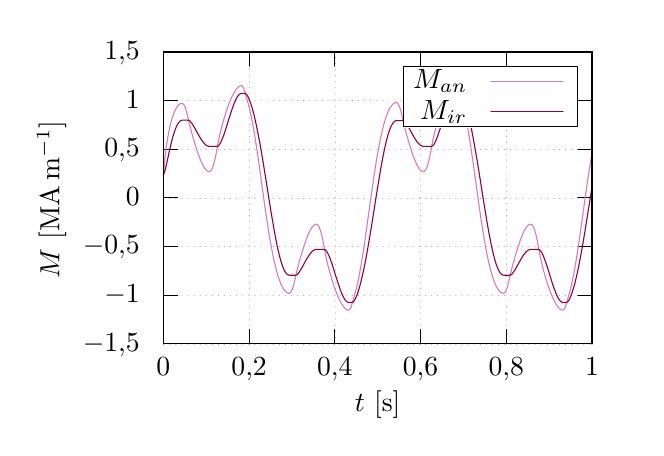
\begin{tikzpicture}[gnuplot]
%% generated with GNUPLOT 5.4p2 (Lua 5.4; terminal rev. Jun 2020, script rev. 114)
%% Fri 23 May 2025 09:04:49 AM -03
\path (0.000,0.000) rectangle (7.500,5.000);
\gpcolor{color=gp lt color axes}
\gpsetlinetype{gp lt axes}
\gpsetdashtype{gp dt axes}
\gpsetlinewidth{0.50}
\draw[gp path] (1.504,0.985)--(6.947,0.985);
\gpcolor{color=gp lt color border}
\gpsetlinetype{gp lt border}
\gpsetdashtype{gp dt solid}
\gpsetlinewidth{1.00}
\draw[gp path] (1.504,0.985)--(1.684,0.985);
\draw[gp path] (6.947,0.985)--(6.767,0.985);
\node[gp node right] at (1.320,0.985) {$-1,5$};
\gpcolor{color=gp lt color axes}
\gpsetlinetype{gp lt axes}
\gpsetdashtype{gp dt axes}
\gpsetlinewidth{0.50}
\draw[gp path] (1.504,1.603)--(6.947,1.603);
\gpcolor{color=gp lt color border}
\gpsetlinetype{gp lt border}
\gpsetdashtype{gp dt solid}
\gpsetlinewidth{1.00}
\draw[gp path] (1.504,1.603)--(1.684,1.603);
\draw[gp path] (6.947,1.603)--(6.767,1.603);
\node[gp node right] at (1.320,1.603) {$-1$};
\gpcolor{color=gp lt color axes}
\gpsetlinetype{gp lt axes}
\gpsetdashtype{gp dt axes}
\gpsetlinewidth{0.50}
\draw[gp path] (1.504,2.220)--(6.947,2.220);
\gpcolor{color=gp lt color border}
\gpsetlinetype{gp lt border}
\gpsetdashtype{gp dt solid}
\gpsetlinewidth{1.00}
\draw[gp path] (1.504,2.220)--(1.684,2.220);
\draw[gp path] (6.947,2.220)--(6.767,2.220);
\node[gp node right] at (1.320,2.220) {$-0,5$};
\gpcolor{color=gp lt color axes}
\gpsetlinetype{gp lt axes}
\gpsetdashtype{gp dt axes}
\gpsetlinewidth{0.50}
\draw[gp path] (1.504,2.838)--(6.947,2.838);
\gpcolor{color=gp lt color border}
\gpsetlinetype{gp lt border}
\gpsetdashtype{gp dt solid}
\gpsetlinewidth{1.00}
\draw[gp path] (1.504,2.838)--(1.684,2.838);
\draw[gp path] (6.947,2.838)--(6.767,2.838);
\node[gp node right] at (1.320,2.838) {$0$};
\gpcolor{color=gp lt color axes}
\gpsetlinetype{gp lt axes}
\gpsetdashtype{gp dt axes}
\gpsetlinewidth{0.50}
\draw[gp path] (1.504,3.456)--(6.947,3.456);
\gpcolor{color=gp lt color border}
\gpsetlinetype{gp lt border}
\gpsetdashtype{gp dt solid}
\gpsetlinewidth{1.00}
\draw[gp path] (1.504,3.456)--(1.684,3.456);
\draw[gp path] (6.947,3.456)--(6.767,3.456);
\node[gp node right] at (1.320,3.456) {$0,5$};
\gpcolor{color=gp lt color axes}
\gpsetlinetype{gp lt axes}
\gpsetdashtype{gp dt axes}
\gpsetlinewidth{0.50}
\draw[gp path] (1.504,4.073)--(4.559,4.073);
\draw[gp path] (6.763,4.073)--(6.947,4.073);
\gpcolor{color=gp lt color border}
\gpsetlinetype{gp lt border}
\gpsetdashtype{gp dt solid}
\gpsetlinewidth{1.00}
\draw[gp path] (1.504,4.073)--(1.684,4.073);
\draw[gp path] (6.947,4.073)--(6.767,4.073);
\node[gp node right] at (1.320,4.073) {$1$};
\gpcolor{color=gp lt color axes}
\gpsetlinetype{gp lt axes}
\gpsetdashtype{gp dt axes}
\gpsetlinewidth{0.50}
\draw[gp path] (1.504,4.691)--(6.947,4.691);
\gpcolor{color=gp lt color border}
\gpsetlinetype{gp lt border}
\gpsetdashtype{gp dt solid}
\gpsetlinewidth{1.00}
\draw[gp path] (1.504,4.691)--(1.684,4.691);
\draw[gp path] (6.947,4.691)--(6.767,4.691);
\node[gp node right] at (1.320,4.691) {$1,5$};
\gpcolor{color=gp lt color axes}
\gpsetlinetype{gp lt axes}
\gpsetdashtype{gp dt axes}
\gpsetlinewidth{0.50}
\draw[gp path] (1.504,0.985)--(1.504,4.691);
\gpcolor{color=gp lt color border}
\gpsetlinetype{gp lt border}
\gpsetdashtype{gp dt solid}
\gpsetlinewidth{1.00}
\draw[gp path] (1.504,0.985)--(1.504,1.165);
\draw[gp path] (1.504,4.691)--(1.504,4.511);
\node[gp node center] at (1.504,0.677) {$0$};
\gpcolor{color=gp lt color axes}
\gpsetlinetype{gp lt axes}
\gpsetdashtype{gp dt axes}
\gpsetlinewidth{0.50}
\draw[gp path] (2.593,0.985)--(2.593,4.691);
\gpcolor{color=gp lt color border}
\gpsetlinetype{gp lt border}
\gpsetdashtype{gp dt solid}
\gpsetlinewidth{1.00}
\draw[gp path] (2.593,0.985)--(2.593,1.165);
\draw[gp path] (2.593,4.691)--(2.593,4.511);
\node[gp node center] at (2.593,0.677) {$0,2$};
\gpcolor{color=gp lt color axes}
\gpsetlinetype{gp lt axes}
\gpsetdashtype{gp dt axes}
\gpsetlinewidth{0.50}
\draw[gp path] (3.681,0.985)--(3.681,4.691);
\gpcolor{color=gp lt color border}
\gpsetlinetype{gp lt border}
\gpsetdashtype{gp dt solid}
\gpsetlinewidth{1.00}
\draw[gp path] (3.681,0.985)--(3.681,1.165);
\draw[gp path] (3.681,4.691)--(3.681,4.511);
\node[gp node center] at (3.681,0.677) {$0,4$};
\gpcolor{color=gp lt color axes}
\gpsetlinetype{gp lt axes}
\gpsetdashtype{gp dt axes}
\gpsetlinewidth{0.50}
\draw[gp path] (4.770,0.985)--(4.770,3.741);
\draw[gp path] (4.770,4.511)--(4.770,4.691);
\gpcolor{color=gp lt color border}
\gpsetlinetype{gp lt border}
\gpsetdashtype{gp dt solid}
\gpsetlinewidth{1.00}
\draw[gp path] (4.770,0.985)--(4.770,1.165);
\draw[gp path] (4.770,4.691)--(4.770,4.511);
\node[gp node center] at (4.770,0.677) {$0,6$};
\gpcolor{color=gp lt color axes}
\gpsetlinetype{gp lt axes}
\gpsetdashtype{gp dt axes}
\gpsetlinewidth{0.50}
\draw[gp path] (5.858,0.985)--(5.858,3.741);
\draw[gp path] (5.858,4.511)--(5.858,4.691);
\gpcolor{color=gp lt color border}
\gpsetlinetype{gp lt border}
\gpsetdashtype{gp dt solid}
\gpsetlinewidth{1.00}
\draw[gp path] (5.858,0.985)--(5.858,1.165);
\draw[gp path] (5.858,4.691)--(5.858,4.511);
\node[gp node center] at (5.858,0.677) {$0,8$};
\gpcolor{color=gp lt color axes}
\gpsetlinetype{gp lt axes}
\gpsetdashtype{gp dt axes}
\gpsetlinewidth{0.50}
\draw[gp path] (6.947,0.985)--(6.947,4.691);
\gpcolor{color=gp lt color border}
\gpsetlinetype{gp lt border}
\gpsetdashtype{gp dt solid}
\gpsetlinewidth{1.00}
\draw[gp path] (6.947,0.985)--(6.947,1.165);
\draw[gp path] (6.947,4.691)--(6.947,4.511);
\node[gp node center] at (6.947,0.677) {$1$};
\draw[gp path] (1.504,4.691)--(1.504,0.985)--(6.947,0.985)--(6.947,4.691)--cycle;
\node[gp node center,rotate=-270] at (0.108,2.838) {$M$ [\si{\mega\ampere\per\meter}]};
\node[gp node center] at (4.225,0.215) {$t$ [\si{\second}]};
\draw[gp path] (4.559,3.741)--(4.559,4.511)--(6.763,4.511)--(6.763,3.741)--cycle;
\gpcolor{rgb color={0.831,0.488,0.735}}
\draw[gp path] (1.504,3.099)--(1.522,3.335)--(1.540,3.485)--(1.559,3.601)--(1.577,3.697)%
  --(1.595,3.777)--(1.613,3.844)--(1.631,3.899)--(1.650,3.944)--(1.668,3.979)--(1.686,4.006)%
  --(1.704,4.025)--(1.722,4.036)--(1.741,4.040)--(1.759,4.030)--(1.777,3.997)--(1.795,3.943)%
  --(1.813,3.871)--(1.832,3.787)--(1.850,3.717)--(1.868,3.651)--(1.886,3.588)--(1.904,3.527)%
  --(1.923,3.469)--(1.941,3.413)--(1.959,3.361)--(1.977,3.314)--(1.996,3.273)--(2.014,3.237)%
  --(2.032,3.209)--(2.050,3.188)--(2.068,3.175)--(2.087,3.171)--(2.105,3.180)--(2.123,3.210)%
  --(2.141,3.261)--(2.159,3.331)--(2.178,3.421)--(2.196,3.525)--(2.214,3.614)--(2.232,3.690)%
  --(2.250,3.761)--(2.269,3.826)--(2.287,3.887)--(2.305,3.944)--(2.323,3.996)--(2.341,4.045)%
  --(2.360,4.090)--(2.378,4.130)--(2.396,4.166)--(2.414,4.196)--(2.432,4.222)--(2.451,4.242)%
  --(2.469,4.256)--(2.487,4.263)--(2.505,4.261)--(2.523,4.233)--(2.542,4.175)--(2.560,4.110)%
  --(2.578,4.047)--(2.596,3.977)--(2.614,3.897)--(2.633,3.807)--(2.651,3.707)--(2.669,3.598)%
  --(2.687,3.481)--(2.705,3.358)--(2.724,3.230)--(2.742,3.099)--(2.760,2.967)--(2.778,2.836)%
  --(2.796,2.707)--(2.815,2.583)--(2.833,2.463)--(2.851,2.351)--(2.869,2.245)--(2.888,2.148)%
  --(2.906,2.059)--(2.924,1.979)--(2.942,1.907)--(2.960,1.844)--(2.979,1.790)--(2.997,1.744)%
  --(3.015,1.706)--(3.033,1.675)--(3.051,1.653)--(3.070,1.637)--(3.088,1.628)--(3.106,1.626)%
  --(3.124,1.642)--(3.142,1.681)--(3.161,1.739)--(3.179,1.816)--(3.197,1.901)--(3.215,1.972)%
  --(3.233,2.038)--(3.252,2.101)--(3.270,2.162)--(3.288,2.220)--(3.306,2.275)--(3.324,2.326)%
  --(3.343,2.372)--(3.361,2.412)--(3.379,2.446)--(3.397,2.472)--(3.415,2.491)--(3.434,2.502)%
  --(3.452,2.504)--(3.470,2.490)--(3.488,2.454)--(3.506,2.399)--(3.525,2.323)--(3.543,2.229)%
  --(3.561,2.126)--(3.579,2.042)--(3.597,1.967)--(3.616,1.899)--(3.634,1.835)--(3.652,1.775)%
  --(3.670,1.719)--(3.688,1.667)--(3.707,1.619)--(3.725,1.576)--(3.743,1.537)--(3.761,1.502)%
  --(3.780,1.473)--(3.798,1.448)--(3.816,1.430)--(3.834,1.418)--(3.852,1.412)--(3.871,1.420)%
  --(3.889,1.455)--(3.907,1.519)--(3.925,1.581)--(3.943,1.646)--(3.962,1.718)--(3.980,1.800)%
  --(3.998,1.893)--(4.016,1.995)--(4.034,2.106)--(4.053,2.225)--(4.071,2.350)--(4.089,2.479)%
  --(4.107,2.610)--(4.125,2.742)--(4.144,2.873)--(4.162,3.000)--(4.180,3.124)--(4.198,3.242)%
  --(4.216,3.353)--(4.235,3.456)--(4.253,3.551)--(4.271,3.638)--(4.289,3.716)--(4.307,3.785)%
  --(4.326,3.846)--(4.344,3.898)--(4.362,3.942)--(4.380,3.979)--(4.398,4.007)--(4.417,4.028)%
  --(4.435,4.042)--(4.453,4.049)--(4.471,4.048)--(4.489,4.026)--(4.508,3.983)--(4.526,3.919)%
  --(4.544,3.838)--(4.562,3.756)--(4.580,3.687)--(4.599,3.622)--(4.617,3.560)--(4.635,3.499)%
  --(4.653,3.442)--(4.671,3.388)--(4.690,3.338)--(4.708,3.294)--(4.726,3.255)--(4.744,3.223)%
  --(4.763,3.198)--(4.781,3.181)--(4.799,3.173)--(4.817,3.174)--(4.835,3.193)--(4.854,3.234)%
  --(4.872,3.294)--(4.890,3.374)--(4.908,3.473)--(4.926,3.572)--(4.945,3.653)--(4.963,3.726)%
  --(4.981,3.794)--(4.999,3.857)--(5.017,3.916)--(5.036,3.970)--(5.054,4.021)--(5.072,4.068)%
  --(5.090,4.110)--(5.108,4.148)--(5.127,4.182)--(5.145,4.210)--(5.163,4.233)--(5.181,4.250)%
  --(5.199,4.260)--(5.218,4.264)--(5.236,4.250)--(5.254,4.208)--(5.272,4.140)--(5.290,4.079)%
  --(5.309,4.013)--(5.327,3.938)--(5.345,3.853)--(5.363,3.758)--(5.381,3.654)--(5.400,3.541)%
  --(5.418,3.420)--(5.436,3.294)--(5.454,3.165)--(5.472,3.033)--(5.491,2.901)--(5.509,2.771)%
  --(5.527,2.644)--(5.545,2.522)--(5.563,2.406)--(5.582,2.297)--(5.600,2.195)--(5.618,2.102)%
  --(5.636,2.018)--(5.655,1.942)--(5.673,1.875)--(5.691,1.816)--(5.709,1.766)--(5.727,1.724)%
  --(5.746,1.690)--(5.764,1.663)--(5.782,1.644)--(5.800,1.632)--(5.818,1.626)--(5.837,1.631)%
  --(5.855,1.659)--(5.873,1.708)--(5.891,1.776)--(5.909,1.861)--(5.928,1.938)--(5.946,2.005)%
  --(5.964,2.070)--(5.982,2.132)--(6.000,2.191)--(6.019,2.248)--(6.037,2.301)--(6.055,2.349)%
  --(6.073,2.393)--(6.091,2.430)--(6.110,2.460)--(6.128,2.483)--(6.146,2.498)--(6.164,2.504)%
  --(6.182,2.499)--(6.201,2.475)--(6.219,2.429)--(6.237,2.363)--(6.255,2.279)--(6.273,2.176)%
  --(6.292,2.083)--(6.310,2.004)--(6.328,1.932)--(6.346,1.866)--(6.364,1.804)--(6.383,1.746)%
  --(6.401,1.692)--(6.419,1.643)--(6.437,1.597)--(6.455,1.556)--(6.474,1.519)--(6.492,1.487)%
  --(6.510,1.460)--(6.528,1.438)--(6.547,1.423)--(6.565,1.414)--(6.583,1.413)--(6.601,1.434)%
  --(6.619,1.484)--(6.638,1.551)--(6.656,1.613)--(6.674,1.681)--(6.692,1.758)--(6.710,1.845)%
  --(6.729,1.943)--(6.747,2.050)--(6.765,2.165)--(6.783,2.287)--(6.801,2.414)--(6.820,2.544)%
  --(6.838,2.676)--(6.856,2.808)--(6.874,2.937)--(6.892,3.063)--(6.911,3.183)--(6.929,3.298)%
  --(6.947,3.405);
\gpcolor{rgb color={0.569,0.000,0.247}}
\draw[gp path] (1.504,3.133)--(1.522,3.174)--(1.540,3.251)--(1.559,3.335)--(1.577,3.419)%
  --(1.595,3.498)--(1.613,3.572)--(1.631,3.637)--(1.650,3.694)--(1.668,3.741)--(1.686,3.777)%
  --(1.704,3.803)--(1.722,3.819)--(1.741,3.825)--(1.759,3.825)--(1.777,3.825)--(1.795,3.825)%
  --(1.813,3.825)--(1.832,3.822)--(1.850,3.806)--(1.868,3.782)--(1.886,3.753)--(1.904,3.722)%
  --(1.923,3.688)--(1.941,3.655)--(1.959,3.622)--(1.977,3.592)--(1.996,3.564)--(2.014,3.540)%
  --(2.032,3.520)--(2.050,3.505)--(2.068,3.496)--(2.087,3.492)--(2.105,3.492)--(2.123,3.492)%
  --(2.141,3.493)--(2.159,3.493)--(2.178,3.493)--(2.196,3.494)--(2.214,3.512)--(2.232,3.543)%
  --(2.250,3.583)--(2.269,3.631)--(2.287,3.684)--(2.305,3.740)--(2.323,3.799)--(2.341,3.857)%
  --(2.360,3.915)--(2.378,3.970)--(2.396,4.021)--(2.414,4.065)--(2.432,4.103)--(2.451,4.133)%
  --(2.469,4.154)--(2.487,4.164)--(2.505,4.166)--(2.523,4.166)--(2.542,4.166)--(2.560,4.154)%
  --(2.578,4.126)--(2.596,4.085)--(2.614,4.035)--(2.633,3.976)--(2.651,3.908)--(2.669,3.832)%
  --(2.687,3.749)--(2.705,3.659)--(2.724,3.563)--(2.742,3.461)--(2.760,3.355)--(2.778,3.245)%
  --(2.796,3.132)--(2.815,3.017)--(2.833,2.901)--(2.851,2.786)--(2.869,2.673)--(2.888,2.562)%
  --(2.906,2.456)--(2.924,2.356)--(2.942,2.263)--(2.960,2.178)--(2.979,2.101)--(2.997,2.035)%
  --(3.015,1.978)--(3.033,1.932)--(3.051,1.898)--(3.070,1.873)--(3.088,1.860)--(3.106,1.856)%
  --(3.124,1.856)--(3.142,1.856)--(3.161,1.856)--(3.179,1.856)--(3.197,1.860)--(3.215,1.877)%
  --(3.233,1.902)--(3.252,1.932)--(3.270,1.963)--(3.288,1.997)--(3.306,2.030)--(3.324,2.062)%
  --(3.343,2.092)--(3.361,2.119)--(3.379,2.142)--(3.397,2.161)--(3.415,2.174)--(3.434,2.182)%
  --(3.452,2.184)--(3.470,2.184)--(3.488,2.184)--(3.506,2.184)--(3.525,2.184)--(3.543,2.184)%
  --(3.561,2.179)--(3.579,2.158)--(3.597,2.124)--(3.616,2.082)--(3.634,2.033)--(3.652,1.979)%
  --(3.670,1.921)--(3.688,1.863)--(3.707,1.804)--(3.725,1.747)--(3.743,1.693)--(3.761,1.644)%
  --(3.780,1.600)--(3.798,1.565)--(3.816,1.537)--(3.834,1.519)--(3.852,1.511)--(3.871,1.510)%
  --(3.889,1.510)--(3.907,1.511)--(3.925,1.528)--(3.943,1.559)--(3.962,1.602)--(3.980,1.655)%
  --(3.998,1.717)--(4.016,1.786)--(4.034,1.864)--(4.053,1.949)--(4.071,2.041)--(4.089,2.138)%
  --(4.107,2.241)--(4.125,2.348)--(4.144,2.459)--(4.162,2.573)--(4.180,2.688)--(4.198,2.804)%
  --(4.216,2.919)--(4.235,3.031)--(4.253,3.141)--(4.271,3.245)--(4.289,3.344)--(4.307,3.435)%
  --(4.326,3.518)--(4.344,3.592)--(4.362,3.657)--(4.380,3.710)--(4.398,3.753)--(4.417,3.785)%
  --(4.435,3.807)--(4.453,3.818)--(4.471,3.820)--(4.489,3.820)--(4.508,3.820)--(4.526,3.820)%
  --(4.544,3.820)--(4.562,3.813)--(4.580,3.793)--(4.599,3.767)--(4.617,3.737)--(4.635,3.704)%
  --(4.653,3.671)--(4.671,3.638)--(4.690,3.606)--(4.708,3.577)--(4.726,3.551)--(4.744,3.529)%
  --(4.763,3.511)--(4.781,3.499)--(4.799,3.493)--(4.817,3.492)--(4.835,3.492)--(4.854,3.492)%
  --(4.872,3.492)--(4.890,3.492)--(4.908,3.492)--(4.926,3.501)--(4.945,3.526)--(4.963,3.562)%
  --(4.981,3.606)--(4.999,3.657)--(5.017,3.711)--(5.036,3.769)--(5.054,3.828)--(5.072,3.887)%
  --(5.090,3.943)--(5.108,3.996)--(5.127,4.044)--(5.145,4.085)--(5.163,4.119)--(5.181,4.144)%
  --(5.199,4.160)--(5.218,4.166)--(5.236,4.166)--(5.254,4.166)--(5.272,4.163)--(5.290,4.141)%
  --(5.309,4.107)--(5.327,4.061)--(5.345,4.007)--(5.363,3.943)--(5.381,3.871)--(5.400,3.791)%
  --(5.418,3.705)--(5.436,3.611)--(5.454,3.513)--(5.472,3.408)--(5.491,3.300)--(5.509,3.188)%
  --(5.527,3.074)--(5.545,2.959)--(5.563,2.843)--(5.582,2.729)--(5.600,2.617)--(5.618,2.509)%
  --(5.636,2.406)--(5.655,2.309)--(5.673,2.219)--(5.691,2.138)--(5.709,2.067)--(5.727,2.005)%
  --(5.746,1.954)--(5.764,1.914)--(5.782,1.884)--(5.800,1.865)--(5.818,1.857)--(5.837,1.856)%
  --(5.855,1.856)--(5.873,1.856)--(5.891,1.856)--(5.909,1.856)--(5.928,1.868)--(5.946,1.889)%
  --(5.964,1.917)--(5.982,1.947)--(6.000,1.980)--(6.019,2.013)--(6.037,2.046)--(6.055,2.077)%
  --(6.073,2.106)--(6.091,2.131)--(6.110,2.152)--(6.128,2.168)--(6.146,2.179)--(6.164,2.184)%
  --(6.182,2.184)--(6.201,2.184)--(6.219,2.184)--(6.237,2.184)--(6.255,2.184)--(6.273,2.184)%
  --(6.292,2.170)--(6.310,2.142)--(6.328,2.104)--(6.346,2.058)--(6.364,2.006)--(6.383,1.950)%
  --(6.401,1.892)--(6.419,1.833)--(6.437,1.775)--(6.455,1.719)--(6.474,1.668)--(6.492,1.621)%
  --(6.510,1.582)--(6.528,1.550)--(6.547,1.527)--(6.565,1.513)--(6.583,1.510)--(6.601,1.510)%
  --(6.619,1.510)--(6.638,1.517)--(6.656,1.542)--(6.674,1.580)--(6.692,1.627)--(6.710,1.685)%
  --(6.729,1.750)--(6.747,1.824)--(6.765,1.906)--(6.783,1.994)--(6.801,2.089)--(6.820,2.189)%
  --(6.838,2.294)--(6.856,2.404)--(6.874,2.516)--(6.892,2.630)--(6.911,2.746)--(6.929,2.861)%
  --(6.947,2.975);
\gpfill{color=gpbgfillcolor} (4.559,3.741)--(6.763,3.741)--(6.763,4.511)--(4.559,4.511)--cycle;
\gpcolor{color=gp lt color border}
\draw[gp path] (4.559,3.741)--(4.559,4.511)--(6.763,4.511)--(6.763,3.741)--cycle;
\node[gp node right] at (5.479,4.318) {\phantom{M}$M_{an}$};
\gpcolor{rgb color={0.831,0.488,0.735}}
\draw[gp path] (5.663,4.318)--(6.579,4.318);
\gpcolor{color=gp lt color border}
\node[gp node right] at (5.479,3.933) {\phantom{M}$M_{ir}$};
\gpcolor{rgb color={0.569,0.000,0.247}}
\draw[gp path] (5.663,3.933)--(6.579,3.933);
\gpcolor{color=gp lt color border}
\draw[gp path] (1.504,4.691)--(1.504,0.985)--(6.947,0.985)--(6.947,4.691)--cycle;
%% coordinates of the plot area
\gpdefrectangularnode{gp plot 1}{\pgfpoint{1.504cm}{0.985cm}}{\pgfpoint{6.947cm}{4.691cm}}
\end{tikzpicture}
%% gnuplot variables

    \vspace{-1cm}
    \caption{HHHHHHHHHHHHHHH}
  \end{minipage}%
\end{figure}

%\newpage

%Uma forma de onda muito comum na elétrica, sendo inclusive a da tensão na rede, é a senoidal. Uma onda senoidal ($V(t)$) é matematicamente dada especificada por
%\begin{equation}
%  V(t) = V_p sen(\omega t) \text{,}
%\end{equation}
%
%\noindent sendo $V_p$ o valor de pico da tensão (ou amplitude) e $\omega = 2\pi f$, sendo $f$ a frequência do sinal.
%
%\exercise Plote 3 períodos $T = f^{-1}$ de uma onda senoidal: a figura \ref{fig_1} apresenta 3 períodos de uma onda senoidal utilizando os parâmetros da tabela \ref{tab_1}.
%
%\begin{table}[!h]
%  %\fontsize{10pt}{10pt}\selectfont
%  \centering
%  \caption{Parâmetros da forma de onda senoidal de tensão}
%  \label{tab_1}
%  \begin{tabular}{ccc}
%    \toprule
%    Parâmetro & Valor \\
%    \midrule
%    Amplitude & $1~\si{\volt}$ \\
%    Frequência & $60~\si{\hertz}$ \\
%    \bottomrule
%  \end{tabular}
%\end{table}
%
%\begin{figure}[!h]
%  \centering
%  \caption{Forma de onda senoidal de tensão}
%  \label{fig_1}
%  \makebox[0pt][c]{\includegraphics[scale=.333333333333333]{v.png}}
%\end{figure}
%
%\exercise Analise matematicamente o comportamento da corrente em um dispositivo indutivo quando nele chaveada um tensão senoidal no instante $V(t) = 0$, $V^\prime(t) > 0$. Considere que esse instante ocorre em $t = 0$. Considere também resistência elétrica desprezível.
%
%A corrente ($I$) em um dispositivo de indutância ($L$), obedece
%\begin{equation} \label{l}
%  \frac{dI}{dt} = \frac{V}{L}\text{.}
%\end{equation}
%
%Integrando a equação \ref{l}, obtemos 
%\begin{equation} \label{l2}
%  I(t) = \int_0^t\frac{V}{L}dt = \frac{V_p}{L} \int_0^t sen(\omega t) dt = \frac{V_p}{L} [-cos(\omega t) + cos(\omega 0)] = -\frac{V_p}{L} cos(\omega t) + \frac{V_p}{L}\text{.}
%\end{equation}
%
%A figura \ref{fig_2} apresenta a forma de onda da corrente considerando-se $L = 1$.
%
%\begin{figure}[!h]
%  \centering
%  \caption{Forma de onda da corrente}
%  \label{fig_2}
%  \makebox[0pt][c]{\includegraphics[scale=.333333333333333]{i.png}}
%\end{figure}
%
%Note que, por conta do valor constante na integral da senoide, obtivemos um \textit{offset} na forma de onda da corrente e um alto valor de pico ($2V_p/L$).


%
%  \newpage
%
%  \item Formas de onda:
%
%  \begin{figure}[h]
%    \centering
%    \begin{subfigure}[t]{.47\textwidth}
%      \includegraphics[width=68mm, right]{vl.png}
%      \caption{$v_L$}
%    \end{subfigure}
%    \begin{subfigure}[t]{.52\textwidth}
%      \centering
%      \includegraphics[width=81mm, right]{ic.png}
%      \caption{$i_C$}
%    \end{subfigure}
%    \begin{subfigure}[t]{.47\textwidth}
%      \centering
%      \includegraphics[width=74.5mm, right]{vc.png}
%      \caption{$v_C$}
%    \end{subfigure}
%    \begin{subfigure}[t]{.52\textwidth}
%      \centering
%      \includegraphics[width=74.5mm, right]{il.png}
%      \caption{$i_L$}
%    \end{subfigure}
%    \caption{Formas de onda no conversor.}
%  \end{figure}
%
%\end{enumerate}
%
%\exercise
%
%Obtenha a equação de ganho estático com perdas. Para tanto, modele as perdas no indutor por uma resistência $R_L$, as perdas nos interruptores por uma resistência $R_{ON}$, e as perdas nos diodos por uma queda de tensão $V_D$.
%
%\begin{enumerate}[(a)]
%
%  \item Etapas de operação:
%
%  \begin{itemize}
%
%    \item Modo 1:
%
%    \begin{center}
%      \begin{tikzpicture}[scale=.9]
%        \ctikzset{bipoles/length=1.26cm}
%        \draw[color=black, thick]
%        (-2.5, 0)
%        to [V, v=$V_i$, invert] (-2.5, 2.5)
%        to [R, l=$R_{ON}$] (0, 2.5)
%        to [R, l=$R_L$] (2.5, 2.5)
%        to [L, l=$L_1$, v=$v_L$] (5, 2.5)
%        to [open] (7.5, 2.5)
%        to [C, l=$C_1$, i>^=$i_C$] (7.5, 0)
%        (7.5, 2.5)
%        to [short] (10, 2.5)
%        to [R, l=$R$, v=$V_o$, label distance=100pt] (10, 0)
%        to [short] (7.5, 0)
%        to [short] (5, 0)
%        to [R, l=$R_{ON}$] (5, 2.5)
%        (5, 0)
%        to [short] (2.5, 0)
%        to [open] (2.5, 2.5)
%        (2.5, 0)
%        to [short] (-2.5, 0);
%      \end{tikzpicture}
%    \end{center}
%  
%    Equações:
%
%    \begin{equation*}
%      v_L = V_i - \left(2R_{ON} + R_L \right) I_L = L_1 \frac{di_L}{dt}
%    \end{equation*}
%
%    \begin{equation*}
%      i_C = -\frac{V_o}{R} = C_1 \frac{dv_C}{dt}
%    \end{equation*}
%
%    \item Modo 2:
%
%    \begin{center}
%      \begin{tikzpicture}[scale=.9]
%        \ctikzset{bipoles/length=1.26cm}
%        \draw[color=black, thick]
%        (-2.5, 0)
%        to [V, v=$V_i$, invert] (-2.5, 2.5)
%        to [open] (0, 2.5)
%        to [R, l=$R_L$] (2.5, 2.5)
%        to [L, l=$L_1$, v=$v_L$] (5, 2.5)
%        to [short] (5, 2.5)
%        to [V, v=$V_D$] (7.5, 2.5)
%        to [C, l=$C_1$, i>^=$i_C$] (7.5, 0)
%        (7.5, 2.5)
%        to [short] (10, 2.5)
%        to [R, l=$R$, v=$V_o$, label distance=100pt] (10, 0)
%        to [short] (7.5, 0)
%        to [short] (0, 0)
%        to [V, v=$V_D$] (0, 2.5)
%        (2.5, 0)
%        to [short] (-2.5, 0);
%      \end{tikzpicture}
%    \end{center}
%
%    Equações:
%
%    \begin{equation*}
%      v_L = -(V_o + 2V_D + R_L I_L) = L_1 \frac{di_L}{dt}
%    \end{equation*}
%
%    \begin{equation*}
%      i_C = I_L -\frac{V_o}{R} = C_1 \frac{dv_C}{dt}
%    \end{equation*}
%
%  \end{itemize}
%
%  \item Ganho estático:
%
%  O ganho estático pode ser encontrado sabendo que, em um período, $\langle v_L \rangle = 0$:
%
%  \begin{equation*}
%    \langle v_L \rangle = \frac{1}{T_s} \left[ \left(V_i - \left(2R_{ON} + R_L \right) I_L \right) D T_s - \left(V_o + 2V_D + R_L I_L \right) (1-D) T_s \right ] = 0 
%  \end{equation*}%
%  \begin{equation*}
%    V_i D - \left(2 R_{ON} D + R_L \right) I_L - \left(1-D \right) V_o - \left(1-D \right) 2 V_D = 0
%  \end{equation*}%
%  \begin{equation*}
%    I_L = \frac{V_o}{\left(1-D \right) R} \text{, } \; \alpha = \frac{2 R_{ON} D + R_L}{\left(1-D \right) R}
%  \end{equation*}
%  \begin{equation*}%
%    V_o = \frac{1}{1-D} \left[ V_i D - \alpha V_o - \left(1-D \right) 2 V_D \right]
%  \end{equation*}
%  \begin{equation*}%
%    V_o = \frac{1}{1 + \frac{\alpha}{1-D}} \left[ \frac{V_i D}{1-D} - 2 V_D \right] = \boxed{\frac{V_i D - 2 \left(1-D \right) V_D}{1-D + \alpha}}
%  \end{equation*}
%
%\end{enumerate}
%
%\exercise
%
%Compare as curvas de ganho estático (ideal e com perdas) com resultados de simulação.
%
%\vspace{.5cm}
%
%\begin{center}
%\begin{minipage}[t]{.3\textwidth}
%  \centering
%
%  Parâmetros:
%
%  \vspace{.5cm}
%
%  \begin{tabular}{|c|c|}
%    \hline
%    $T_s$ & 20 $\mathrm{\mu}$s\\
%    \hline
%    $V_i$ & 100 V\\
%    \hline
%    $P_o$ & 100 W\\
%    \hline
%    $\Delta V_o$ & 0,1 \%\\
%    \hline
%    $\Delta I_L$ & 10 \%\\
%    \hline
%    $V_D$ & 1 V\\
%    \hline
%    $R_L$ & 100 m$\Omega$\\
%    \hline
%    $R_{ON}$ & 100 m$\Omega$\\
%    \hline
%  \end{tabular}
%\end{minipage}%
%\begin{minipage}[t]{.5\textwidth}
%  \centering
%  Projetando para $D = 0,5$:
%
%  \vspace{-.2cm}
%
%  \begin{equation*}
%    R = \frac{V_o^2}{P_o} = \frac{100^2}{100} = 100 \; \Omega 
%  \end{equation*}%
%  \begin{equation*}
%    C_1 = \frac{D T_s V_o}{\Delta V_o R} = \frac{0,5 \cdot 20 \cdot 10^{-6} \cdot 100}{0,1 \cdot 100} = 100 \; \mathrm{\mu F}
%  \end{equation*}%
%  \begin{equation*}
%    L_1 = \frac{D T_s V_i}{\Delta I_L} = \frac{0,5 \cdot 20 \cdot 10^{-6} \cdot 100}{0,1 \cdot \frac{100}{\left(1-0,5 \right) 100}} = 5 \; \mathrm{mH}
%  \end{equation*}
%\end{minipage}%
%\end{center}
%
%\vspace{.5cm}
%
%Comparando:
%
%\begin{figure}[h]
%  \centering
%  \includegraphics[width=136mm]{G.png}
%  \caption{Comparação dos ganhos.}
%\end{figure}

\end{document}
